\documentclass{article}

% Language setting
% Replace `english' with e.g. `spanish' to change the document language
\usepackage[english]{babel}

% Set page size and margins
% Replace `letterpaper' with `a4paper' for UK/EU standard size
\usepackage[a4paper,top=2cm,bottom=2cm,left=3cm,right=3cm,marginparwidth=1.75cm]{geometry}

% Useful packages
\usepackage{amsmath}
\allowdisplaybreaks
% Equation numbers as <section>.<n> (e.g. the 2nd numbered equation in
% Section 3 prints as (3.2)). Resets the equation counter at each \section.
\numberwithin{equation}{section}

\usepackage{amsthm}
\newtheorem{theorem}{Theorem}
\newtheorem{lemma}{Lemma}
\newtheorem{corollary}{Corollary}
\newtheorem{claim}{Claim}
\newtheorem{approximation}{Approximation}
% remark environment (upright body), added for the Model-B2 singular-limit
% discussion (playbook task C3); independent counter like the others.
\theoremstyle{remark}
\newtheorem{remark}{Remark}
\theoremstyle{plain}

\usepackage{amssymb}
\usepackage{graphicx}
% float must be loaded before hyperref: [H] floats otherwise emit duplicate
% pdfTeX destination identifiers (one per figure/table in the document).
\usepackage{float}
\usepackage[colorlinks=true, allcolors=blue]{hyperref}

\usepackage{tikz}
\usetikzlibrary{arrows.meta, positioning, matrix}

\usepackage{xcolor}



\usepackage{booktabs}
\usepackage{multirow}

\newcommand{\tpi}{\widetilde{\pi}}
\newcommand{\tP}{\widetilde{P}}

% Head-of-line variants (constant rate 1{n1>=1}); superscript H = "head-of-line".
% Math-mode only: use inside $...$.
\newcommand{\BH}{B_2^{\mathrm{H}}}
\newcommand{\CH}{C_2^{\mathrm{H}}}

% Computed metrics for the Results/Comparison prose (generated by
% Code/compute_derived_metrics.py; see task D1). Numbers are macros, not hardcoded.
% Auto-generated by Code/compute_derived_metrics.py -- DO NOT EDIT BY HAND.
% Derived metrics for the Results/Comparison prose. \input this file.

\newcommand{\lossCtwoFifty}{0.166}
\newcommand{\lossCHFifty}{0.156}
\newcommand{\lossCtwoSeventy}{0.232}
\newcommand{\lossCHSeventy}{0.212}
\newcommand{\lossCtwoNinety}{0.297}
\newcommand{\lossCHNinety}{0.266}
\newcommand{\lossCtwoCanon}{0.232}
\newcommand{\lossCHCanon}{0.212}

\newcommand{\lossSysCtwoFifty}{0.071}
\newcommand{\lossSysCHFifty}{0.067}
\newcommand{\lossSysCtwoSeventy}{0.099}
\newcommand{\lossSysCHSeventy}{0.091}
\newcommand{\lossSysCtwoNinety}{0.127}
\newcommand{\lossSysCHNinety}{0.114}
\newcommand{\lossSysCtwoCanon}{0.099}

\newcommand{\lossCtwoThetaLow}{0.044}
\newcommand{\lossCtwoThetaHigh}{0.468}

\newcommand{\condWoneA}{0.9944}
\newcommand{\uncondWoneA}{1.0000}
\newcommand{\fracServedA}{1.000}
\newcommand{\condWoneBtwo}{0.4433}
\newcommand{\uncondWoneBtwo}{0.5151}
\newcommand{\fracServedBtwo}{0.742}
\newcommand{\condWoneCtwo}{0.3863}
\newcommand{\uncondWoneCtwo}{0.4639}
\newcommand{\fracServedCtwo}{0.768}
\newcommand{\condWoneCH}{0.4478}
\newcommand{\uncondWoneCH}{0.5303}
\newcommand{\fracServedCH}{0.788}

\newcommand{\alphaStarA}{0.10}
\newcommand{\ratioPeakA}{0.300}
\newcommand{\alphaStarBtwo}{0.10}
\newcommand{\ratioPeakBtwo}{0.188}
\newcommand{\alphaStarCtwo}{0.90}
\newcommand{\ratioPeakCtwo}{0.357}
\newcommand{\alphaStarBH}{0.10}
\newcommand{\ratioPeakBH}{0.193}
\newcommand{\alphaStarCH}{0.90}
\newcommand{\ratioPeakCH}{0.395}

\newcommand{\ENoneBtwoFifty}{0.0767}
\newcommand{\ENoneBHFifty}{0.0833}
\newcommand{\gapENoneFifty}{0.0067}
\newcommand{\ENoneBtwoSeventy}{0.1545}
\newcommand{\ENoneBHSeventy}{0.1750}
\newcommand{\gapENoneSeventy}{0.0205}
\newcommand{\ENoneBtwoNinety}{0.2626}
\newcommand{\ENoneBHNinety}{0.3115}
\newcommand{\gapENoneNinety}{0.0489}

\newcommand{\PNGetwoAFifty}{0.0230}
\newcommand{\PNGetwoBtwoFifty}{0.0072}
\newcommand{\PNGetwoCtwoFifty}{0.0067}
\newcommand{\PNGetwoBHFifty}{0.0102}
\newcommand{\PNGetwoCHFifty}{0.0095}
\newcommand{\PNGetwoASeventy}{0.0630}
\newcommand{\PNGetwoBtwoSeventy}{0.0193}
\newcommand{\PNGetwoCtwoSeventy}{0.0174}
\newcommand{\PNGetwoBHSeventy}{0.0280}
\newcommand{\PNGetwoCHSeventy}{0.0255}
\newcommand{\PNGetwoANinety}{0.1339}
\newcommand{\PNGetwoBtwoNinety}{0.0399}
\newcommand{\PNGetwoCtwoNinety}{0.0348}
\newcommand{\PNGetwoBHNinety}{0.0595}
\newcommand{\PNGetwoCHNinety}{0.0527}

\newcommand{\premiumASeventy}{3.33}
\newcommand{\premiumBtwoSeventy}{7.18}
\newcommand{\premiumCtwoSeventy}{3.75}
\newcommand{\premiumANinety}{10.00}
\newcommand{\premiumBtwoNinety}{22.38}
\newcommand{\premiumCtwoNinety}{6.30}

\newcommand{\offeredFifty}{0.50}
\newcommand{\throughputAFifty}{0.5000}
\newcommand{\throughputBtwoFifty}{0.5000}
\newcommand{\throughputBHFifty}{0.5000}
\newcommand{\throughputCtwoFifty}{0.4644}
\newcommand{\throughputCHFifty}{0.4667}
\newcommand{\lostflowCtwoFifty}{0.0356}
\newcommand{\lostflowCHFifty}{0.0333}
\newcommand{\offeredSeventy}{0.70}
\newcommand{\throughputASeventy}{0.7000}
\newcommand{\throughputBtwoSeventy}{0.7000}
\newcommand{\throughputBHSeventy}{0.7000}
\newcommand{\throughputCtwoSeventy}{0.6304}
\newcommand{\throughputCHSeventy}{0.6364}
\newcommand{\lostflowCtwoSeventy}{0.0696}
\newcommand{\lostflowCHSeventy}{0.0636}
\newcommand{\offeredNinety}{0.90}
\newcommand{\throughputANinety}{0.9000}
\newcommand{\throughputBtwoNinety}{0.9000}
\newcommand{\throughputBHNinety}{0.9000}
\newcommand{\throughputCtwoNinety}{0.7854}
\newcommand{\throughputCHNinety}{0.7975}
\newcommand{\lostflowCtwoNinety}{0.1146}
\newcommand{\lostflowCHNinety}{0.1025}

\newcommand{\piZeroAFifty}{0.5000}
\newcommand{\piZZAFifty}{0.2500}
\newcommand{\ENAFifty}{0.5000}
\newcommand{\ENtwoAFifty}{0.3636}
\newcommand{\EWoneAFifty}{0.6364}
\newcommand{\EWtwoAFifty}{1.2727}
\newcommand{\piZeroBtwoFifty}{0.5000}
\newcommand{\piZZBtwoFifty}{0.2500}
\newcommand{\ENBtwoFifty}{0.5000}
\newcommand{\ENtwoBtwoFifty}{0.4233}
\newcommand{\EWoneBtwoFifty}{0.3578}
\newcommand{\EWtwoBtwoFifty}{1.4817}
\newcommand{\piZeroCtwoFifty}{0.5356}
\newcommand{\piZZCtwoFifty}{0.2678}
\newcommand{\ENCtwoFifty}{0.3233}
\newcommand{\ENtwoCtwoFifty}{0.2521}
\newcommand{\EWoneCtwoFifty}{0.3323}
\newcommand{\EWtwoCtwoFifty}{0.8823}
\newcommand{\piZeroBHFifty}{0.5000}
\newcommand{\piZZBHFifty}{0.2500}
\newcommand{\ENBHFifty}{0.5000}
\newcommand{\ENtwoBHFifty}{0.4167}
\newcommand{\EWoneBHFifty}{0.3889}
\newcommand{\EWtwoBHFifty}{1.4583}
\newcommand{\piZeroCHFifty}{0.5333}
\newcommand{\piZZCHFifty}{0.2667}
\newcommand{\ENCHFifty}{0.3370}
\newcommand{\ENtwoCHFifty}{0.2593}
\newcommand{\EWoneCHFifty}{0.3630}
\newcommand{\EWtwoCHFifty}{0.9074}
\newcommand{\ENoneAFifty}{0.1364}
\newcommand{\ENoneCtwoFifty}{0.0712}
\newcommand{\ENoneCHFifty}{0.0778}
\newcommand{\piZeroASeventy}{0.3000}
\newcommand{\piZZASeventy}{0.2100}
\newcommand{\ENASeventy}{1.6333}
\newcommand{\ENtwoASeventy}{1.3333}
\newcommand{\EWoneASeventy}{1.0000}
\newcommand{\EWtwoASeventy}{3.3333}
\newcommand{\piZeroBtwoSeventy}{0.3000}
\newcommand{\piZZBtwoSeventy}{0.2100}
\newcommand{\ENBtwoSeventy}{1.6333}
\newcommand{\ENtwoBtwoSeventy}{1.4788}
\newcommand{\EWoneBtwoSeventy}{0.5151}
\newcommand{\EWtwoBtwoSeventy}{3.6970}
\newcommand{\piZeroCtwoSeventy}{0.3696}
\newcommand{\piZZCtwoSeventy}{0.2587}
\newcommand{\ENCtwoSeventy}{0.8358}
\newcommand{\ENtwoCtwoSeventy}{0.6967}
\newcommand{\EWoneCtwoSeventy}{0.4639}
\newcommand{\EWtwoCtwoSeventy}{1.7417}
\newcommand{\piZeroBHSeventy}{0.3000}
\newcommand{\piZZBHSeventy}{0.2100}
\newcommand{\ENBHSeventy}{1.6333}
\newcommand{\ENtwoBHSeventy}{1.4583}
\newcommand{\EWoneBHSeventy}{0.5833}
\newcommand{\EWtwoBHSeventy}{3.6458}
\newcommand{\piZeroCHSeventy}{0.3636}
\newcommand{\piZZCHSeventy}{0.2545}
\newcommand{\ENCHSeventy}{0.9015}
\newcommand{\ENtwoCHSeventy}{0.7424}
\newcommand{\EWoneCHSeventy}{0.5303}
\newcommand{\EWtwoCHSeventy}{1.8561}
\newcommand{\ENoneASeventy}{0.3000}
\newcommand{\ENoneCtwoSeventy}{0.1392}
\newcommand{\ENoneCHSeventy}{0.1591}
\newcommand{\piZeroANinety}{0.1000}
\newcommand{\piZZANinety}{0.0900}
\newcommand{\ENANinety}{8.1000}
\newcommand{\ENtwoANinety}{7.5349}
\newcommand{\EWoneANinety}{1.4651}
\newcommand{\EWtwoANinety}{14.6511}
\newcommand{\piZeroBtwoNinety}{0.1000}
\newcommand{\piZZBtwoNinety}{0.0900}
\newcommand{\ENBtwoNinety}{8.1000}
\newcommand{\ENtwoBtwoNinety}{7.8374}
\newcommand{\EWoneBtwoNinety}{0.6808}
\newcommand{\EWtwoBtwoNinety}{15.2394}
\newcommand{\piZeroCtwoNinety}{0.2146}
\newcommand{\piZZCtwoNinety}{0.1931}
\newcommand{\ENCtwoNinety}{2.1537}
\newcommand{\ENtwoCtwoNinety}{1.9245}
\newcommand{\EWoneCtwoNinety}{0.5941}
\newcommand{\EWtwoCtwoNinety}{3.7421}
\newcommand{\piZeroBHNinety}{0.1000}
\newcommand{\piZZBHNinety}{0.0900}
\newcommand{\ENBHNinety}{8.1000}
\newcommand{\ENtwoBHNinety}{7.7884}
\newcommand{\EWoneBHNinety}{0.8077}
\newcommand{\EWtwoBHNinety}{15.1442}
\newcommand{\piZeroCHNinety}{0.2025}
\newcommand{\piZZCHNinety}{0.1823}
\newcommand{\ENCHNinety}{2.4844}
\newcommand{\ENtwoCHNinety}{2.2084}
\newcommand{\EWoneCHNinety}{0.7157}
\newcommand{\EWtwoCHNinety}{4.2941}
\newcommand{\ENoneANinety}{0.5651}
\newcommand{\ENoneCtwoNinety}{0.2292}
\newcommand{\ENoneCHNinety}{0.2760}

\newcommand{\premiumBHSeventy}{6.25}
\newcommand{\premiumCHSeventy}{3.50}
\newcommand{\premiumBHNinety}{18.75}
\newcommand{\premiumCHNinety}{6.00}

\newcommand{\EWtwoBtwoInflationSeventy}{10.9}
\newcommand{\ENoneBtwoReductionSeventy}{48.5}
\newcommand{\ENoneBHReductionSeventy}{41.7}


% TODO-confirm: working title (candidate 1 of 3 proposed to the author). Alternatives:
%  (2) Two-Class Priority M/M/1 Queues with Jockeying and Abandonment:
%      A Unified Probability-Generating-Function Framework
%  (3) Stationary Queue-Length Analysis of Non-Preemptive Priority M/M/1 Queues
%      under Jockeying and Reneging: Exact PGFs and an Obstruction Taxonomy
\title{Exact Generating-Function Analysis of a Two-Class Non-Preemptive Priority
\texorpdfstring{$M/M/1$}{M/M/1} Queue with Jockeying and Abandonment}
\author{Victor Dominguez Sainz}

\begin{document}
\tableofcontents
\newpage
\maketitle

\begin{abstract}

We study the stationary queue-length distribution of a two-class, non-preemptive priority $M/M/1$ queue augmented with two waiting-room mechanisms: \emph{jockeying}, in which a waiting customer switches to the other queue, and \emph{abandonment}, in which a waiting customer leaves the system. Jockeying conserves the total number of customers, whereas abandonment does not, and combining both yields a model (Model-$X$) that is analytically intractable. We therefore present a collection of simpler models: Model-$A$ (baseline), Model-$B$ (bidirectional jockeying), Model-$B_2$ (jockeying from the priority class to the non-priority class) and Model-$C_2$ (abandonments in the priority class). We also study two head-of-the-line models: Model-$B_2^H$ (only the first customer in the priority queue can jockey) and Model-$C_2^H$ (only the first customer in the priority queue can abandon).

The central object is the bivariate Probability Generating Function (PGF) $P(x,y)$ of the two queue lengths, obtained by analytical and, where the structure allows, probabilistic arguments. The purpose of this work is to present a unified framework for deriving the functional equation of each model and to expose the mathematical challenges intrinsic to each. Model-$A$ is classical and collapses to an algebraic expression by finding a kernel root inside the unit circle; Model-$B_2$ is solved by imposing analyticity at an interior point and Model-$C_2$ by imposing boundedness inside the unit circle. The head-of-the-line models, like the baseline Model-$A$, also yield an algebraic expression for the PGF. Two models are left open: Model-$B$ reduces to an integral expression for the PGF involving a Volterra-type integral equation, and Model-$X$ compounds this with nonlinear characteristic curves.

Every closed form is validated against a truncated continuous-time Markov Chain (CTMC) that recovers the baseline model as the mechanism rates vanish. The comparison reveals a key difference between jockeying and abandonment: the former merely redistributes delay between classes, whereas the latter substantially shortens the queue lengths.
\end{abstract}


\section{Introduction}

\subsection*{Motivation}

Priority queues arise naturally wherever a common server must satisfy heterogeneous demand. The primary motivation for this thesis is healthcare operations, specifically the management of waiting lists for elderly-care facilities, where medical severity dictates a user's —hereafter \emph{customer}— priority class. Here prolonged waiting may itself alter the system's dynamics: a lack of appropriate care can deteriorate a waiting customer's health, leading them to change priority status (jockeying) or leave the system (abandonment), whether to seek alternative care or through death. Despite this motivation, the work is fundamentally modelling-driven: we characterise the long-run behaviour of queueing systems in which jockeying and/or abandonment play a role.

This thesis analyses a $2$-class $M/M/1$ queue with non-preemptive priority: each class arrives according to a Poisson process (rates $\lambda_1$ and $\lambda_2$), service times are exponential at a common rate $\mu$, and the single server completes the current service even when a higher-priority customer arrives. To this we add the mechanisms of jockeying and abandonment. The model and its mechanisms are described in more detail in \S\ref{sec:model_x}.

How these two mechanisms interact within a priority discipline, and how that interaction affects the difficulty of obtaining a closed-form Probability Generating Function (PGF), is the main focus of this thesis.

\subsection*{The analytical challenge}

In full generality, the bivariate PGF for Model-$X$ satisfies a functional equation with terms of three kinds: algebraic coefficients, partial derivatives in $x$ —from jockeying and abandonment in class-$1$— and partial derivatives in $y$ —from the same mechanisms in class-$2$. When both kinds of derivative term are present, the equation belongs to a family of integro-differential equations whose solution would require more advanced tools. The problem is moreover asymmetric: derivative terms from the non-priority class complicate it more than those from the priority class alone.

We therefore solve less complex models obtained by setting some of the jockeying and abandonment parameters to zero. Table~\ref{tab:model_overview_intro} lists the models studied here and indicates whether a PGF expression is obtained for each:
\begin{table}[H]
\centering
\renewcommand{\arraystretch}{1.3}
\label{tab:model_overview_intro}
    \begin{tabular}{clll}
        \hline
            \textbf{Model} & \textbf{Active mechanism} & \textbf{Equation type} & \textbf{Status} \\
            \hline
            A     & none                                    & algebraic PGF equation & solved  \\
            B     & bidirectional jockeying                 & PDE, Volterra family   & open \\
            X     & jockeying and abandonment               & PDE, transcendental characteristics & open \\
            B$_2$   & one-way jockeying ($1\to2$)           & ODE in $x$, Kummer     & solved \\
            $\BH$ & one-way jockeying, head-of-line       & algebraic PGF equation & solved \\
            C$_2$   & class-1 abandonment                   & ODE in $x$, Kummer     & solved \\
            $\CH$ & class-1 abandonment, head-of-line     & algebraic PGF equation & solved \\
        \hline
    \end{tabular}
    \caption{Models studied in this thesis, with the active mechanism, the resulting functional-equation type, and the solution status. The head-of-line variants $\BH$ and $\CH$ restrict the mechanism to the customer at the head of Queue~1, which
collapses the derivative term to an algebraic one and renders the model solvable in closed
form.}
\end{table}
Some models —notably Model-$X$ and Model-$B$— are left incomplete because they involve derivative terms in $y$; others, such as a potential Model-$B_1$, Model-$C$ or Model-$C_1$, are not considered for the same reason, as they all reduce to a Volterra integral equation lying beyond the scope of this thesis. Model-$B$ serves as our representative example of how such problems reduce to that integral equation; the remaining models are solvable. The last two entries, Models~$\BH$ and~$\CH$ (\S\S\ref{sec:model_b21} and~\ref{sec:model_c21}), are \emph{head-of-line} simplifications in which only the customer at the head of Queue~1 may jockey or abandon. The mechanism then acts at the constant rate $\gamma_1\mathbf 1_{\{n_1\ge1\}}$ or $\theta_1\mathbf 1_{\{n_1\ge1\}}$ rather than the length-proportional $\gamma_1 n_1$ or $\theta_1 n_1$, so the fundamental equation stays algebraic and is solved by the Kernel Method exactly as in Model-$A$.

\subsection*{Methods}

Three complementary proof strategies are used throughout.

\emph{Kernel method / ODE with integrating factor}. For Model-$A$, which has no derivative terms, the algebraic coefficient of $P(x,y)$ vanishes on a curve (the \emph{kernel}); evaluating the equation there determines the remaining unknowns. Model-$B_2$ and Model-$C_2$, which do carry derivative terms in $x$, reduce to a first-order linear ODE in $x$ with an explicit integrating factor, and their unknowns follow from a regularity argument at a singularity of that factor. We present both strategies together, as they share the same underlying idea: the latter extends the former to the case where the unknowns are independent of the derivative terms and can be taken outside the integral.

\emph{Probabilistic argument via Pollaczek--Khinchine and the effective service time}. For Model-$A$ and Model-$C_2$, class-$2$ arrivals are Poisson, so the PASTA property holds and we can apply the Pollaczek--Khinchine formula together with the \emph{effective service time} seen by a class-$2$ customer. This is an $M/G/1$ queue whose service times equal the busy period of the class-$1$ subsystem —an $M/M/1$ queue for Model-$A$ and an $M/M/1+M$ system for Model-$C_2$. In both cases the argument independently confirms the analytic results. Since jockeying destroys the Poisson structure, it does not apply to the other models.

\emph{Partial PGF (PPGF) in the alternative state space $\widetilde{S}$}. For the baseline Model-$A$ we introduce an alternative state space indexed by the number of class-$2$ customers —whose distribution is hard— and the total number of customers —which is easy, since the total is conserved and behaves like a regular $M/M/1$ queue. This yields a PPGF with a non-homogeneous term. Cohen's recursion argument \cite{cohen1956delay} was developed for the regular state space; we explore, with limited success, the challenges of carrying it over to this alternative space and assess whether Cohen's trick can deliver a feasible rough approximation.

\subsection*{Structure of the thesis}

Section~\ref{sec:literature} reviews the relevant literature and Section~\ref{sec:prelim} collects the probabilistic and analytic background used throughout this work. Section~\ref{sec:model_x} defines the full model, Model-$X$, and derives the general balance equations and the fundamental PGF equations, both for the regular and the alternative state space. The analysis then proceeds from baseline to synthesis: Section~\ref{sec:model_a} solves the baseline Model-$A$ in closed form; Section~\ref{sec:model_b} shows that bidirectional jockeying (Model-$B$) reduces the problem to a Volterra-type integral equation and is left open. Sections~\ref{sec:model_b2} and~\ref{sec:model_c2} then recover tractability in the one-way-jockeying (Model-$B_2$) and class-1-abandonment (Model-$C_2$) specialisations, while Sections~\ref{sec:model_b21} and~\ref{sec:model_c21} show how the head-of-line variants, Models~$\BH$ and~$\CH$, collapse the functional equation to an algebraic one solved in closed form. Finally, Section~\ref{sec:comparison} compares the solved models, Section~\ref{sec:results} presents the numerical validation and performance metrics, and Section~\ref{sec:conclusion} concludes by abstracting the obstruction taxonomy and setting out the future work.

\section{Literature}\label{sec:literature}

The study of two-class priority queues with jockeying and abandonment sits at the intersection of three well-developed streams: the exact generating-function analysis of non-preemptive priority queues, the theory of queues with customer impatience (abandonment), and the theory of jockeying and dynamic priority changes. The applied motivation throughout is the management of access to care ---elderly-care waiting lists, emergency departments, and transplant registries--- in which the two mechanisms studied here carry direct clinical readings: a waiting patient whose condition deteriorates changes priority class (jockeying), while one who leaves the list by death or transfer abandons the system (abandonment). This thesis contributes an exact, single-server treatment that admits jockeying and abandonment within a unified bivariate-PGF framework, filling a gap that the multi-server and approximate literature has so far left open.

% ── §2.1 ──────────────────────────────────────────────────────────────────────
\subsection*{Non-preemptive priority queues: exact queue-length analysis}

The expected waiting times of the non-preemptive priority $M/M/1$ queue are standard textbook material~\cite{adan2002queueing}; the exact \emph{queue-length} analysis is where the generating-function tradition begins. The direct methodological ancestor of this work is Cohen~\cite{cohen1956delay}, who studied a single server loaded by two independent Poisson streams under non-preemptive priority and introduced a partial-generating-function recursion that resolves the lower-priority queue length by transforming only one coordinate of the joint distribution while keeping the other discrete; we refer to this device as the ``Cohen trick''. It is exactly the device reused, in modern notation, in the partial-PGF analysis of Model-$A$ on the total-count state space (\S\ref{ssec:A:Stilde}). The stationary queue-length law of the two-class non-preemptive $M/M/1$ priority queue ---the content of Theorem~\ref{thm:A:PGF} (Model-$A$)--- is in this sense classical, recoverable by several routes.

The most recent exact closed-form treatment of the non-preemptive priority queue is that of Zuk \& Kirszenblat~\cite{zuk2023explicit}, who obtain the joint and marginal queue-length distributions of a non-preemptive $M/M/c$ queue with two priority classes and a common service rate by generating-function methods and a quadratic recurrence; their single-server specialisation ($c=1$) coincides with Model-$A$.

% ── §2.2 ──────────────────────────────────────────────────────────────────────
\subsection*{Priority queues with abandonment}

Abandonment enters queueing theory through the Erlang-A ($M/M/c+M$) model, in which each waiting customer holds an independent exponential patience clock; the modern treatment and its heavy-traffic scaling are due to Garnett et al.~\cite{garnett2002designing}. The analytic signature of impatience is well documented: per-customer patience clocks make the transition rates state-inhomogeneous, so the generating-function solutions, where they close at all, close in terms of hypergeometric series.

Kapodistria~\cite{kapodistria2011synchronized} exhibits this pattern most clearly in a single-server queue with \emph{synchronised} abandonments, in which all waiting customers abandon simultaneously, each with probability $p$, at Poisson opportunity epochs. The stationary law is solved exactly through basic ($q$-)hypergeometric series, and in the no-synchronisation limit $p\to0^+$ it recovers the $M/M/1+M$ queue-length PGF as a ratio of Kummer functions: precisely the special-function structure that carries the boundary function of Model-$C_2$.

Exact stationary results for priority queues \emph{with} abandonment are scarce, and those available concern multi-server systems. Jouini \& Roubos~\cite{jouini2014multiple} treat an $M/M/s+M$ queue with two non-preemptive classes in which the classes are statistically identical ---a common service rate and a common patience distribution, so that the classes differ only in their priority level. They derive Laplace--Stieltjes transforms for conditional and unconditional waiting times together with the probabilities of service and of abandonment; this is the multi-server analogue of Model-$C_2$, but with the waiting time, not the queue-length PGF, as its object. Where exact transforms are unavailable the literature turns to fluid and diffusion approximations or to many-server asymptotics~\cite{zeltyn2005callcenters}; the exact Erlang-A stationary law itself is expressed through confluent hypergeometric and incomplete-gamma functions, the same special-function structure that appears, at finite scale, in the closed form for Model-$C_2$.

The exact multi-server priority results that do exist involve no abandonment at all: Wang et al.~\cite{wang2015mmc} analyse a preemptive $M/M/c$ queue with class-dependent service rates and no impatience, and Zuk \& Kirszenblat~\cite{zuk2023explicit} a non-preemptive $M/M/c$ queue, likewise without impatience. Model-$C_2$ therefore appears to be the first exact, single-server, queue-length treatment of \emph{class-asymmetric} abandonment, with impatience acting on the priority class alone. The clinical reading that licenses this asymmetry is long-standing: Zenios~\cite{zenios1999modeling} models the organ-transplant waiting list as a queue whose abandonment mechanism is patient mortality, precisely the regime in which losing high-priority demand is the outcome of interest.

% ── §2.3 ──────────────────────────────────────────────────────────────────────
\subsection*{Jockeying and priority changes}

The closest predecessor on the jockeying side is de Waal~\cite{deWaal1992approximate}, who studies an $M/G/1$ priority queue in which impatient customers \emph{may change priority class} while waiting. de Waal's analysis is approximate by necessity rather than by choice: with general service times an exact analysis is out of reach, and the paper delivers Laplace--Stieltjes-based \emph{approximations} of the waiting-time distributions rather than an exact stationary law. The healthcare incarnation of the same idea is the model of Hu, Chan \& Dong~\cite{huchandong2022proactive}, who let customers transition between a moderate and an urgent class as their condition deteriorates or improves and characterise a near-optimal $c\mu/\theta$-type scheduling index in heavy traffic; the system is multi-server and its results are asymptotic, so it too is approximate in the sense of Table~\ref{tab:literature}.

A complementary strand studies dynamic rather than static priority: Stanford et al.~\cite{stanford2014accumulating} analyse the \emph{accumulating-priority} $M/G/1$ queue, in which each class earns priority linearly in its waiting time so that older customers eventually overtake newer ones, and derive exact waiting-time distributions through a maximum-priority process and Laplace--Stieltjes transforms. Accumulating priority is a continuous-time analogue of the discrete, rate-$\gamma_i$ jockeying studied here; like the present work it is exact and single-server, but its object is the sojourn time rather than the bivariate queue-length PGF.

Model-$B_2$ is the exact counterpart of this ``priority-change'' literature. It retains the deterioration mechanism ---a waiting class-$1$ customer relocates to the class-$2$ queue at rate $\gamma_1$--- and pays for exactness with the single-server, Markovian, one-directional restriction. In return it produces a closed-form boundary function in place of an approximation.

% ── §2.4 ──────────────────────────────────────────────────────────────────────
\subsection*{Methodological lineage}

The functional-equation technique used in Sections~\ref{sec:model_b2} and~\ref{sec:model_c2} belongs to the kernel-method and boundary-value tradition for two-dimensional Markovian queues. The systematic theory ---reducing a bivariate balance equation to the curve on which its kernel vanishes, and from there to a boundary-value problem for the unknown boundary functions--- is developed by Fayolle, Iasnogorodski \& Malyshev~\cite{fayolle1999random} for random walks in the quarter-plane. That approach still delivers explicit two-class results: Devos, Walraevens, Fiems \& Bruneel~\cite{devos2020alternating} obtain the closed-form joint queue-length distribution of a discrete-time two-class queue with randomly alternating service by analysing the kernel of just such a functional equation and determining its two unknown boundary functions through analytic continuation.

The arguments of this thesis are elementary, one-dimensional instances of that method. In Model-$B_2$ the boundary function is fixed by demanding \emph{analyticity} of the PGF at the interior point where the kernel root meets the diagonal (\S\ref{sec:model_b2}), and in Model-$C_2$ by demanding mere \emph{boundedness} at the unit-disc boundary (\S\ref{sec:model_c2}); both select the analytic solution of the reduced equation, exactly the role the boundary conditions play in the general theory.

Two narrower tools recur. The confluent hypergeometric (Kummer) function that carries the Model-$C_2$ boundary function is the same special function through which the Erlang-A and reneging-queue stationary laws are expressed~\cite{zeltyn2005callcenters,kapodistria2011synchronized,dlmf}; and the selection of the decaying solution of the three-term recurrence behind the partial-PGF analysis is governed by Pincherle's theorem, for which we cite the recurrence-relation treatment of Gautschi~\cite{gautschi1967computational} alongside the DLMF~\cite{dlmf}.

% ── §2.6 ──────────────────────────────────────────────────────────────────────
\subsection*{Position of this thesis}

\begin{table}[H]
\centering
\caption{Literature overview: models and mechanisms.
\checkmark~= present, --~= absent, $\approx$~= approximate only.}
\label{tab:literature}
\renewcommand{\arraystretch}{1.3}
\footnotesize
\begin{tabular}{lcccccc}
\hline
\textbf{Reference} & \textbf{Servers} & \textbf{Non-preem.} & \textbf{Jockeying}
  & \textbf{Aband.} & \textbf{Queue-len.} & \textbf{Exact} \\
\hline
Cohen (1956)                      & 1   & \checkmark & -- & --         & \checkmark & \checkmark \\
de Waal (1992)                    & 1   & \checkmark & \checkmark & --  & --         & $\approx$ \\
Jouini \& Roubos (2014)           & $c$ & \checkmark & -- & \checkmark & --         & \checkmark \\
Wang et al.\ (2015)               & $c$ & --         & -- & --         & \checkmark & \checkmark \\
Stanford et al.\ (2014)           & 1   & \checkmark & \checkmark & --  & --         & \checkmark \\
Zuk \& Kirszenblat (2023)         & $c$ & \checkmark & -- & --         & \checkmark & \checkmark \\
Hu, Chan \& Dong (2022)           & $c$ & \checkmark & \checkmark & \checkmark & --   & $\approx$ \\
\hline
\textbf{This thesis (Model-$A$)}    & \textbf{1} & \checkmark & -- & --  & \checkmark & \checkmark \\
\textbf{This thesis (Model-$B_2$)}& \textbf{1} & \checkmark & \checkmark & -- & \checkmark & \checkmark \\
\textbf{This thesis (Model-$C_2$)}& \textbf{1} & \checkmark & -- & \checkmark & \checkmark & \checkmark \\
\hline
\end{tabular}
\end{table}

Table~\ref{tab:literature} places this work against its closest neighbours, and reading it by row makes the gap precise. The Cohen (1956) row is the single-server, exact, non-preemptive queue-length baseline with neither extra mechanism ---the ancestor of Model-$A$. de Waal (1992) adds jockeying (priority change) at a single server, but its analysis is approximate and concerns waiting times rather than queue lengths. Jouini \& Roubos (2014) add abandonment exactly, but at $c$ servers, for statistically identical classes, and again for waiting times. Wang et al.\ (2015) is exact and queue-length-focused, yet multi-server, preemptive, and mechanism-free. Stanford et al.\ (2014) is single-server and exact with a dynamic-priority (jockeying-like) mechanism ---the closest analogue of Model-$B_2$ in the table--- but its object is the sojourn time. Zuk \& Kirszenblat (2023) is the exact multi-server queue-length result whose $c=1$ case is Model-$A$, with neither jockeying nor abandonment. Hu, Chan \& Dong (2022) carries both mechanisms ---jockeying-as-deterioration and abandonment--- and is in that sense the richest model in the table, but it is multi-server and offers no exact results. The pattern is symptomatic of the multi-server literature as a whole: once $c>1$ is combined with jockeying or abandonment, the analysis moves to approximations and asymptotics, so that exact, mechanism-rich analysis is essentially a single-server phenomenon.

No row above combines the exact bivariate queue-length PGF with either jockeying or abandonment ---which is precisely the column pattern of the three ``This thesis'' rows. The gap can therefore be stated in one sentence: prior to this work there is no exact, single-server, queue-length analysis that places non-preemptive priority together with jockeying or abandonment inside a single PGF framework.

The limits of these claims must be stated with equal precision. The framework is unified but not complete: the full model (Model-$X$, Remark~\ref{rem:B:modelX}), in which jockeying and abandonment act together, and the bidirectional-jockeying model (Model-$B$, \S\ref{sec:model_b}) are left open. For each of these, this thesis characterises the analytical obstruction and reduces the problem to a Volterra-type integral equation, providing partial results rather than a closed form. The exact contributions are confined to the three ``This thesis'' rows of Table~\ref{tab:literature} ---the baseline Model-$A$, the one-way jockeying Model-$B_2$, and the class-1 abandonment Model-$C_2$, together with their head-of-line simplifications. The claim is exactness and unification at a single server with one mechanism active at a time; it is explicitly not a solution of the combined or bidirectional problems, which remain, as in the multi-server literature, beyond exact reach.

\section{Preliminaries}\label{sec:prelim}

This section contains some background material referenced throughout the derivations throughout the thesis. By introducing the building blocks in this section, allowing the subsequent the presented arguments to remain focused on their primary intention. Having some known results as preliminaries will help us keep our derivations cleaner.

The central mathematical object in our derivations will be the (P)PGF of the model in question, as well as the idle probability of the system for some corollaries.


\subsection{\texorpdfstring{$M/M/1$}{M/M/1} queue}\label{ssec:mm1}

The model described here is the canonical $M/M/1$ queue, well studied in multiple textbooks and manuals and considered the absolute foundation of queueing theory. Here, we will use \cite{adan2002queueing} as our reference, but there is a lot of good quality literature and sources about it. 
Customers arrive at the system according to a Poisson process —i.e., the inter-arrival times are exponentially distributed with parameter $\lambda$—, service times are exponentially distributed with parameter $\mu$, and a single server operates in first-come-first-serve (FCFS) —also known as first-in-first-out (FIFO)— order. The system is stable if and only if the system's load $\rho = \lambda/\mu < 1$. 

Let $\pi_n$ be the limiting probability of finding $n$ customers in the system. Under stability, the detailed balance equations $\lambda\,\pi_n = \mu\,\pi_{n+1}$ ($n \geq 0$) together with the normalisation $\sum_{n=0}^{\infty}\pi_n=1$ give us the geometric steady-state distribution of the number of customers in the system:
\begin{equation}
    \pi_n = (1-\rho)\,\rho^n, \quad n \ge 0. \label{eq:mm1:steadystate}
\end{equation}
By the PASTA property (\S\ref{ssec:priority}), this also corresponds to the distribution seen by the arriving customers. Let $L$ be the random variable that tells us how many customers—including the one that might be in service—are in the system. The expected number of customers in the system is the following:
\begin{equation*}
    \mathbb{E}[L] = \frac{\rho}{1-\rho}.
\end{equation*}
From this, the expected sojourn time $W$—the time that elapses between a customer's arrival and their departure after service completion—is derived by Little's Law ($\mathbb{E}[L] = \lambda\mathbb{E}[W]$):
\begin{equation*}
    \mathbb{E}[W] = \frac{\mathbb{E}[L]}{\lambda} = \frac{1/\mu}{1-\rho}.
\end{equation*}

Another concept, more rare but highly relevant for the content that will be discussed in this thesis, is the Busy Period ($BP$) of the system, i.e., the time elapsed between the arrival of a customer to an idle system and the departure of a customer who leaves the system empty again after service completion. The Laplace-Stieltjes Transform (LST) and the expectation of this system's busy period are known:
\begin{align}
    \widetilde{BP}(s) &= \frac{(\mu+\lambda+s) - \sqrt{(\mu+\lambda+s)^2 - 4\mu\lambda}}{2\lambda},\label{eq:mm1:bp_lst} \\
    \mathbb{E}[BP]    &= \frac{1}{\mu(1-\rho)}. \label{eq:mm1:bp_mean}
\end{align}

% ─────────────────────────────────────────────────────────────────────────────
\subsection{\texorpdfstring{$M/M/1{+}M$}{M/M/1+M} queue (Erlang-A)}\label{ssec:erlangA}

Another relevant queueing model for this thesis is the so-called $M/M/1+M$ model, also known as the \emph{Erlang A} model. It's based on the $M/M/1$ queue —Poisson arrivals at a rate $\lambda$ and exponentially distributed waiting times with parameter $\mu$-, but adds customer impatience to it: each waiting customer can independently abandon at an exponentially distributed waiting time with parameter $\theta$. The key difference of this model with respect to the $M/M/1$ is that the $M/M/1+M$ does not require $\rho=\lambda / \mu \leq 1$ to be stable: it is positive recurrent for all $\lambda, \mu, \theta > 0$.

The steady state distribution follows, naturally, from its balance equations. At state $n \geq 0$ —for $n$ being the number of customers in the \emph{system}— we have
\begin{equation}
    \lambda\,\pi_n = (\mu + n\theta)\,\pi_{n+1}, \qquad n \ge 0.
    \label{eq:erlangA:balance}
\end{equation}
Iterating yields
\begin{equation}
    \pi_n = \pi_0\,\frac{(\lambda/\theta)^n}{(\mu/\theta)^{(n)}} \quad n \ge 0;
    \label{eq:erlangA:steadystate}
    \quad \text{where} \quad a^{(n)} = a(a+1)\cdots(a+n-1)
\end{equation}
Normalisation gives the non-trivial idle probability $\pi_0 = [{}_1F_1(1;\,\mu/\theta;\,\lambda/\theta)]^{-1}$ (see \S\ref{ssec:kummer} for the Kummer function ${}_1F_1$).

The \emph{Busy Period} of the $M/M/1+M$ defined here is far more complex than the one expressed in the $M/M/1$ queueing system. The LST and the expectation are given by
\begin{align}
    \begin{split}
    \widetilde{B}(s) = \cfrac{\mu}{\lambda_1+\mu+s
      -\cfrac{\lambda_1(\mu+\theta_1)}{\lambda_1+\mu+\theta_1+s
      -\cfrac{\lambda_1(\mu+2\theta_1)}{\lambda_1+\mu+2\theta_1+s-\dotsb}}},
    \label{eq:erlangA:bp_lst}
    \end{split} \\
    \begin{split}
        \mathbb{E}[B] = \dots
        \label{eq:erlangA:bp_exp}
    \end{split}
\end{align}
% TODO: Fill in the expected busy period
% TODO: Explain its integral representation and its Kummer representation

% ─────────────────────────────────────────────────────────────────────────────
\subsection{Pollaczek--Khinchine formula}\label{ssec:pk}

The $M/G/1$ queue —explained in \cite{adan2002queueing}— is a single-server queue with Poisson arrivals at a rate $\lambda$ but with generally distributed i.i.d.\ service times $B$ with mean $\mathbb{E}[B]$

The $M/G/1$ queue~\cite{adan2002queueing} is a single-server queue with Poisson arrivals
at rate $\lambda$ and generally distributed i.i.d.\ service times $B$ with mean and LST $\widetilde{B}(s) = \mathbb{E}[e^{-sB}]$. 
For stability purposes, the system load $\rho = \lambda\,\mathbb{E}[B] < 1$ is required.
Under these two conditions —Poisson arrivals and stability— the Pollaczek--Khinchine (PK) formula
gives the PGF of the stationary number of customers in the system:
\begin{equation}
    L(z) \;=\; \frac{(1-\rho_B)(1-z)\,\widetilde{B}(\lambda(1-z))}{\widetilde{B}(\lambda(1-z)) - z}.
    \label{eq:pk:pgf}
\end{equation}

% ─────────────────────────────────────────────────────────────────────────────
\subsection{Confluent hypergeometric function}\label{ssec:kummer}

The \emph{Kummer confluent hypergeometric function of the first kind} function will come up in some of the derivations of this thesis, and it reads as follows:
\begin{equation}
    {}_1F_1(a;\,b;\,z) \;=\;
        \sum_{n=0}^{\infty} \frac{a^{(n)}}{b^{(n)}\,n!}\,z^n,
    \qquad a^{(n)} = \prod_{k=0}^{n-1}(a+k),\quad a^{(0)}=1,
    \label{eq:kummer:series}
\end{equation}
where $b$ is not $0$ or a negative integer —i.e. $b \notin \{0,-1,-2,\dots\}$— and the series converges for all
$z\in\mathbb{C}$.
The function ${}_1F_1(a;\,b;\,z)$ is the unique solution of \emph{Kummer's equation}~\cite{dlmf}:
\begin{equation}
    z\,u'' + (b - z)\,u' - a\,u = 0, \label{eq:kummer:ode}
\end{equation}
normalized by ${}_1F_1(a;\,b;\,0) = 1$. The \emph{Kummer series} (Equation \eqref{eq:kummer:series}) converges
for all $z\in\mathbb{C}$ and $b \notin \{0,-1,-2,\ldots\}$.

For this thesis, two identities related to it are used.
First, the \emph{Euler integral representation}, for $a,b>0$ we have:
\begin{equation}
    {}_1F_1(a;\,a+b;\,z) \;=\; \frac{1}{B(a,b)} \int_0^1 t^{a-1}(1-t)^{b-1} e^{zt}\,dt, 
    \label{eq:kummer:euler}
\end{equation}
where $B$ is the \emph{Beta distribution} $B(a,b)=\Gamma(a)\Gamma(b)/\Gamma(a+b)$, and $\Gamma$ is the \emph{Gamma function}.
Secondly, the \emph{Contiguous-function ratio}:
\begin{equation}
    \frac{{}_1F_1(a+1;\,b;\,z)}{{}_1F_1(a;\,b;\,z)}.
    \label{eq:kummer:ratio}
\end{equation}


% ─────────────────────────────────────────────────────────────────────────────
\subsection{First-order linear ODEs and PDEs}\label{ssec:ode}

Since jockeying and abandoning add state-dependent rates to our systems, we will have to deal with derivative terms to solve for our PGF's. Here follow some introductions to the methods employed to solve diverse typeS of ODE's and PDE's that will play a role in this thesis.

\subsubsection{Integrating factor (variation of parameters)}

This method is standard to tackle —for each fixed $y—$ a \emph{first-order linear ODE in $x$}, and leads to a closed-form solution, in our case, for $P(x,y)$. Such an equation has standard form
\begin{equation}
    \frac{dP}{dx} + p(x;\,y)\,P \;=\; q(x;\,y). \label{eq:ode:standard}
\end{equation}
The integratimg factor $\mu_I(x;y)$, defined by $\mu_I(x;y) = \exp\bigl(\int_0^x p(t;y)\,dt\bigr)$, converts the standard form (Equation \eqref{eq:ode:standard}) to $\frac{d}{dx}[P\cdot\mu_I] = q\cdot\mu_I$, yielding
\begin{equation}
    P(x,y) \;=\; \frac{1}{\mu_I(x;\,y)}
        \left[C(y) + \int_0^x q(t;\,y)\,\mu_I(t;\,y)\,dt\right].
    \label{eq:ode:variation}
\end{equation}
For $P$ bounded, $\mu_I(0;y)=0$, we have $C(y)=0$, giving
\begin{equation}
    P(x,y) \;=\; \frac{1}{\mu_I(x;\,y)}
        \int_0^x q(t;\,y)\,\mu_I(t;\,y)\,dt.
    \label{eq:ode:variation}
\end{equation}


\subsubsection{Method of characteristics}\label{sssec:moc}

This method is standard for solving a \emph{first-order linear PDE in both $x$ and $y$}, simultaneously. The Method of Characteristics reduces such an equation to a family of ODE's along the so-called \emph{characteistic curve} in the $(x,y)$-plane, and each of those collapse to an ODE in a single parameter, namely $t$. The general solution, thus, is obtained by parameterising one variable in terms of the other and integrating along the characteristics. this, together with an arbitrary function determined by the boundary data, yields a general solution.

A PDE of the form
\begin{equation*}
    a \frac{\partial P}{\partial x} + b \frac{\partial P}{\partial y} = cP + d
\end{equation*}
is solved by tracing the \emph{characteristic curve} —$(x(t),y(t))$, satisfying
\begin{equation}
    \frac{dx}{dt} = a, \quad \frac{dy}{dt} = b.
\end{equation}
Along each of these curves, the function $P(x(t), y(t))$ satisfies:
\begin{equation}
    \frac{dP}{dt} = cP + d
\end{equation}
which is an ODE in the single variable $t$.


\section{The general model and its fundamental equation}\label{sec:model_x}

This section defines the general two-class system with both jockeying and abandonment, which we call \emph{Model-$X$}; the simpler variants studied in the later sections are recovered from it as special cases.

The model is an $M/M/1$ queue with two priority classes. Customers are served First-Come, First-Served (FCFS) within their own class, and class-$1$ (the priority class) has non-preemptive priority over class-$2$: a service in progress is never interrupted, so a class-$2$ customer in service is not displaced by an arriving class-$1$ customer. The server is work-conserving: it is never idle while a customer is present. Beyond these basic dynamics, Model-$X$ adds two queue-leaving mechanisms. First, \emph{jockeying}: a waiting customer leaves its own queue to \emph{join the other queue}, at per-customer rate $\gamma_1$ for direction $1\to2$ and $\gamma_2$ for $2\to1$, so the total number of customers is preserved. Second, \emph{abandonment} (reneging): a waiting customer leaves the \emph{system} at per-customer rate $\theta_i$, decreasing the total by one. Concretely, each waiting class-$i$ customer (not the one in service) holds an independent $\mathrm{Exp}(\theta_i)$ patience clock and abandons when it expires. This is precisely the linear-reneging mechanism of the $M/M/1+M$ queue from \S\ref{ssec:erlangA}.

In Kendall's notation this is an $M/M/1$-type model: Poisson arrivals, exponentially distributed service times, and a single server. Throughout, the parameters are:
\begin{itemize}
    \item $\lambda_1, \lambda_2$: Poisson arrival rates of classes $1$ and $2$, respectively; the total arrival rate is $\lambda=\lambda_1+\lambda_2$;
    \item $\mu$: exponential service rate of a customer, regardless of class;
    \item $\rho_i = \frac{\lambda_i}{\mu}$: system load of class $i \in \{1,2\}$; the total system load is $\rho=\frac{\lambda}{\mu}$;
    \item $\gamma_1, \gamma_2$: per-customer jockeying rates from Class $1\to2$ and $2\to1$, respectively; jockeying transfers a customer between queues, preserving the total number of customers;
    \item $\theta_1, \theta_2$: per-customer abandonment (reneging) rates from classes $1$ and $2$, respectively; abandonment removes a customer from the system, reducing the total by one.
\end{itemize}
The two class arrival streams are independent Poisson processes, and they are independent of the system's internal exponential service, jockeying and abandonment clocks, so they satisfy the lack-of-anticipation assumption of the PASTA property (\S\ref{ssec:priority}). By Poisson \emph{superposition} the merged arrival stream is itself Poisson at rate $\lambda$, and each class stream is an i.i.d.\ $\lambda_i/\lambda$ \emph{thinning} of the merger, so PASTA applies to the aggregate state and to each class separately.

To define the stochastic processes that drive this system, we introduce the following random variables:
\begin{itemize}
    \item $\mathcal{B}:$ binary indicator for the server being idle or busy, $\mathcal{B}\in \{0,1\}$;
    \item $N_1, N_2:$ number of customers of class $1$ and $2$, respectively, in their respective queues;
    \item $N:$ total number of customers in the queues.
\end{itemize}
Note that $N_1$, $N_2$ and $N$ count customers in the \emph{queues}, not the \emph{system}. Because the service rate $\mu$ is common to both classes, the \emph{memorylessness} of the exponential service time makes the residual service of the customer in progress $\mathrm{Exp}(\mu)$ regardless of its class; the class of the in-service customer therefore does not influence the future evolution of the queue lengths, and the state descriptor need not record it. Accordingly, we write the idle state as $(0)$ and all other states as $(n_1,n_2)$, so that $(0,0)$ implies that the server is busy while both queues are empty. Formally,
\begin{equation}
    S := \{(0)\} \cup \{ (n_1,n_2) \mid n_1,n_2 \geq 0 \}.
    \label{eq:gen:state_space_S}
\end{equation}
For the partial-PGF analysis we additionally use an auxiliary state space $\widetilde{S}$, which tracks only $n_2$ and the total $n = n_1 + n_2$, subject to $n \geq n_2 \geq 0$:
\begin{equation}
    \widetilde{S} := \{(0)\} \cup \{ (n_2,n) \mid n \geq n_2 \geq 0 \}.
    \label{eq:gen:state_space_Stilde}
\end{equation}

Assuming positive recurrence, so that the limiting distribution exists, we define the long-run probabilities of finding the system in each state:
\begin{itemize}
    \item $\pi_0$ for the idle state $(0)$, it belongs to both spaces $S$ and $\widetilde{S}$;
    \item $\pi(n_1,n_2)$ for states $(n_1,n_2) \in S$, where $n_1,n_2 \geq 0$;
    \item $\widetilde{\pi}(n_2,n)$ for states $(n_2,n) \in \widetilde{S}$, where $n \geq n_2 \geq 0$.
\end{itemize}

The simpler variants are recovered from Model-$X$ by setting the appropriate parameters to zero, as summarised in Table~\ref{tab:model_family}:
\begin{table}[H]
    \centering
    \begin{tabular}{cccl}
        \hline
        Model & Jockeying & Abandonment & Parameter values \\
        \hline
        $X$  & both ($1\!\leftrightarrow\!2$) & both ($1,2$)       & $\gamma_i \geq 0,\ \theta_i \geq 0$ \quad (general) \\
        $A$  & none                            & none               & $\gamma_1=\gamma_2=0,\ \theta_1=\theta_2=0$ \\
        $B$  & both ($1\!\leftrightarrow\!2$) & none               & $\gamma_i \geq 0,\ \theta_1=\theta_2=0$ \\
        $B_2$ & $1\!\to\!2$ only                & none               & $\gamma_1 \geq 0,\ \gamma_2=0,\ \theta_1=\theta_2=0$ \\
        $C_2$ & none                            & class $1$ only     & $\theta_1 \geq 0,\ \theta_2=0,\ \gamma_1=\gamma_2=0$ \\
        \hline
        $\BH$ & $1\!\to\!2$, head-of-line       & none                    & $\gamma_1\,\mathbf{1}_{\{n_1\ge1\}}>0,\ \gamma_2=\theta_1=\theta_2=0$ \\
        $\CH$ & none                            & class $1$, head-of-line & $\theta_1\,\mathbf{1}_{\{n_1\ge1\}}>0,\ \gamma_1=\gamma_2=\theta_2=0$ \\
        \hline
    \end{tabular}
    \caption{Nested family of models. Model-$X$ is the parent; Models~$A$, $B$, $B_2$ and $C_2$
    are obtained by restricting the jockeying directions and the abandoning classes. The two
    head-of-line variants $\BH$ and $\CH$ are listed separately, as their mechanism involves the indicator $\mathbf{1}_{\{n_1\ge1\}}$ rather than being proportional to the queue length.}
    \label{tab:model_family}
    \par\smallskip
\end{table}

Figure~\ref{fig:models-queue-overview} gives a visual overview of Model-$X$ and each variant we consider. It omits the two head-of-line variants, which are less conventional and for which such a diagram would add little:
\begin{figure}[H]
    \centering
    \resizebox{\textwidth}{!}{%
        % Two-column overview of all five models.
%
% Left column  : Model X (scale 0.75), vertically spanning the full grid height.
% Right column : 2×2 grid of submodels (scale 0.38), row-pitch 3.2 units.
%
%   [ Model X ]  [ Model A  |  Model B  ]
%   [         ]  [ Model B₂ |  Model C₂ ]
%
% No legend — arrow conventions are explained in the caption.
%
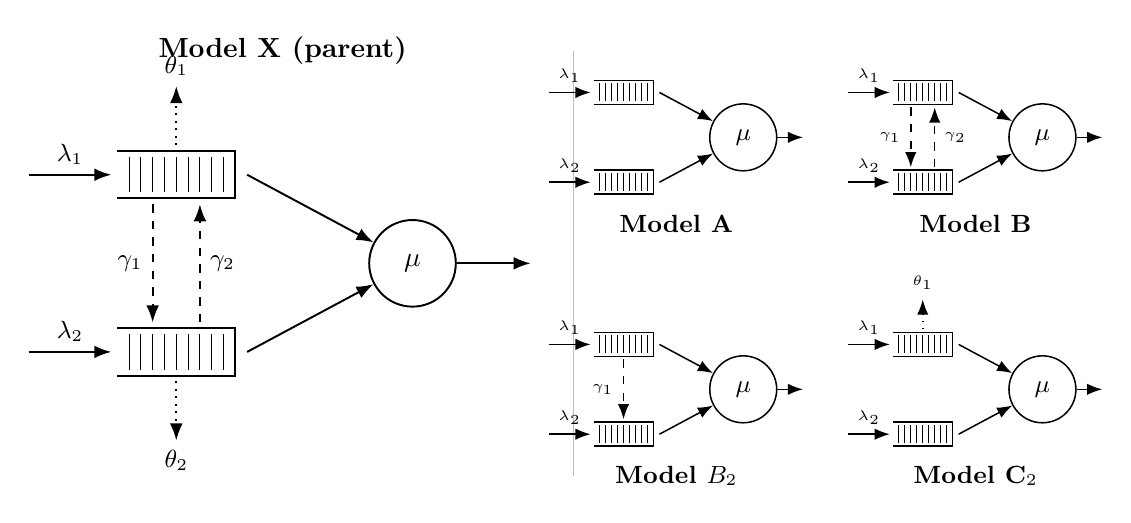
\begin{tikzpicture}[>=Latex]

% ─────────────────────────────────────────────────────────────────────────────
% LEFT COLUMN: Model X
%
% Local coords: x ∈ [−1.5, 7], y ∈ [−3, 3]  (span 8.5 × 6)
% Scale 0.75 → physical 6.375 × 4.5.
% Vertical centre of right grid (see below): y_centre ≈ 1.6
% → shift_y = 1.6  so local y=0 (server) aligns with grid midpoint.
% → shift_x = 1.0  so left edge of diagram lands near x=0.
% ─────────────────────────────────────────────────────────────────────────────
\begin{scope}[shift={(1.0, 1.6)}, scale=0.75, line width=0.7pt]
    % Queue 1 (top, Class-1, priority)
    \draw (0,1.9)--(2,1.9)--(2,1.1)--(0,1.1);
    \foreach \x in {0.2,0.4,...,1.8}{\draw[line width=0.35pt](\x,1.8)--(\x,1.2);}
    \draw[->](-1.5,1.5)--(-0.1,1.5) node[midway,above,font=\small]{$\lambda_1$};
    \draw[->,dotted](1,2.0)--(1,3.0) node[above,font=\small]{$\theta_1$};
    % Queue 2 (bottom, Class-2)
    \draw (0,-1.1)--(2,-1.1)--(2,-1.9)--(0,-1.9);
    \foreach \x in {0.2,0.4,...,1.8}{\draw[line width=0.35pt](\x,-1.2)--(\x,-1.8);}
    \draw[->](-1.5,-1.5)--(-0.1,-1.5) node[midway,above,font=\small]{$\lambda_2$};
    \draw[->,dotted](1,-2.0)--(1,-3.0) node[below,font=\small]{$\theta_2$};
    % Jockeying
    \draw[->,dashed](0.6,1.0)--(0.6,-1.0) node[midway,left,font=\small]{$\gamma_1$};
    \draw[->,dashed](1.4,-1.0)--(1.4,1.0) node[midway,right,font=\small]{$\gamma_2$};
    % Server
    \node[draw,circle,minimum size=1.1cm,font=\normalsize](sX) at (5,0){$\mu$};
    \draw[->](2.2,1.5)--(sX);
    \draw[->](2.2,-1.5)--(sX);
    \draw[->](sX)--(7,0);
\end{scope}
% Label above Model X
\node[font=\normalsize\bfseries] at (3.1, 4.3) {Model~X (parent)};

% Thin vertical separator between columns
\draw[gray!50, thin] (6.8, -1.1) -- (6.8, 4.3);

% ─────────────────────────────────────────────────────────────────────────────
% RIGHT COLUMN: 2×2 grid of submodels (scale 0.38, line width 0.55pt)
%
% Row 1 (top):    A at x-shift 7.05,  B  at x-shift 10.85
% Row 2 (bottom): B₂ at x-shift 7.05, C₂ at x-shift 10.85
% Row y-shifts:   top row 3.2,  bottom row 0.0
% Vertical centre of grid: (−1.9×0.38 + 3.2 + 1.9×0.38) / 2 ≈ 1.6  ← matches Model X
% ─────────────────────────────────────────────────────────────────────────────

% ── Model A (top-left) ───────────────────────────────────────────────────────
\begin{scope}[shift={(7.05, 3.2)}, scale=0.38, line width=0.55pt]
    \draw (0,1.9)--(2,1.9)--(2,1.1)--(0,1.1);
    \foreach \x in {0.2,0.4,...,1.8}{\draw[line width=0.3pt](\x,1.8)--(\x,1.2);}
    \draw[->](-1.5,1.5)--(-0.1,1.5) node[midway,above,font=\tiny]{$\lambda_1$};
    \draw (0,-1.1)--(2,-1.1)--(2,-1.9)--(0,-1.9);
    \foreach \x in {0.2,0.4,...,1.8}{\draw[line width=0.3pt](\x,-1.2)--(\x,-1.8);}
    \draw[->](-1.5,-1.5)--(-0.1,-1.5) node[midway,above,font=\tiny]{$\lambda_2$};
    \node[draw,circle,minimum size=0.85cm,font=\small](sA) at (5,0){$\mu$};
    \draw[->](2.2,1.5)--(sA); \draw[->](2.2,-1.5)--(sA); \draw[->](sA)--(7,0);
\end{scope}
\node[font=\small\bfseries] at (8.10, 2.10) {Model~A};

% ── Model B (top-right) ──────────────────────────────────────────────────────
\begin{scope}[shift={(10.85, 3.2)}, scale=0.38, line width=0.55pt]
    \draw (0,1.9)--(2,1.9)--(2,1.1)--(0,1.1);
    \foreach \x in {0.2,0.4,...,1.8}{\draw[line width=0.3pt](\x,1.8)--(\x,1.2);}
    \draw[->](-1.5,1.5)--(-0.1,1.5) node[midway,above,font=\tiny]{$\lambda_1$};
    \draw (0,-1.1)--(2,-1.1)--(2,-1.9)--(0,-1.9);
    \foreach \x in {0.2,0.4,...,1.8}{\draw[line width=0.3pt](\x,-1.2)--(\x,-1.8);}
    \draw[->](-1.5,-1.5)--(-0.1,-1.5) node[midway,above,font=\tiny]{$\lambda_2$};
    \draw[->,dashed](0.6,1.0)--(0.6,-1.0) node[midway,left,font=\tiny]{$\gamma_1$};
    \draw[->,dashed](1.4,-1.0)--(1.4,1.0) node[midway,right,font=\tiny]{$\gamma_2$};
    \node[draw,circle,minimum size=0.85cm,font=\small](sB) at (5,0){$\mu$};
    \draw[->](2.2,1.5)--(sB); \draw[->](2.2,-1.5)--(sB); \draw[->](sB)--(7,0);
\end{scope}
\node[font=\small\bfseries] at (11.90, 2.10) {Model~B};

% ── Model B₂ (bottom-left) ───────────────────────────────────────────────────
\begin{scope}[shift={(7.05, 0.0)}, scale=0.38, line width=0.55pt]
    \draw (0,1.9)--(2,1.9)--(2,1.1)--(0,1.1);
    \foreach \x in {0.2,0.4,...,1.8}{\draw[line width=0.3pt](\x,1.8)--(\x,1.2);}
    \draw[->](-1.5,1.5)--(-0.1,1.5) node[midway,above,font=\tiny]{$\lambda_1$};
    \draw (0,-1.1)--(2,-1.1)--(2,-1.9)--(0,-1.9);
    \foreach \x in {0.2,0.4,...,1.8}{\draw[line width=0.3pt](\x,-1.2)--(\x,-1.8);}
    \draw[->](-1.5,-1.5)--(-0.1,-1.5) node[midway,above,font=\tiny]{$\lambda_2$};
    \draw[->,dashed](1.0,1.0)--(1.0,-1.0) node[midway,left,font=\tiny]{$\gamma_1$};
    \node[draw,circle,minimum size=0.85cm,font=\small](sB2) at (5,0){$\mu$};
    \draw[->](2.2,1.5)--(sB2); \draw[->](2.2,-1.5)--(sB2); \draw[->](sB2)--(7,0);
\end{scope}
\node[font=\small\bfseries] at (8.10, -1.10) {Model~$B_2$};

% ── Model C₂ (bottom-right) ──────────────────────────────────────────────────
\begin{scope}[shift={(10.85, 0.0)}, scale=0.38, line width=0.55pt]
    \draw (0,1.9)--(2,1.9)--(2,1.1)--(0,1.1);
    \foreach \x in {0.2,0.4,...,1.8}{\draw[line width=0.3pt](\x,1.8)--(\x,1.2);}
    \draw[->](-1.5,1.5)--(-0.1,1.5) node[midway,above,font=\tiny]{$\lambda_1$};
    \draw[->,dotted](1,2.0)--(1,3.0) node[above,font=\tiny]{$\theta_1$};
    \draw (0,-1.1)--(2,-1.1)--(2,-1.9)--(0,-1.9);
    \foreach \x in {0.2,0.4,...,1.8}{\draw[line width=0.3pt](\x,-1.2)--(\x,-1.8);}
    \draw[->](-1.5,-1.5)--(-0.1,-1.5) node[midway,above,font=\tiny]{$\lambda_2$};
    \node[draw,circle,minimum size=0.85cm,font=\small](sC2) at (5,0){$\mu$};
    \draw[->](2.2,1.5)--(sC2); \draw[->](2.2,-1.5)--(sC2); \draw[->](sC2)--(7,0);
\end{scope}
\node[font=\small\bfseries] at (11.90, -1.10) {Model~C$_2$};

\end{tikzpicture}
%
    }
    \caption{Physical queue layout for Model-$X$ (left) and its four specialisations (right, $2\times2$ grid). In all models, Queue~$1$ (top buffer) has non-preemptive priority over Queue~$2$. Solid arrows are for Poisson arrivals ($\lambda_i$) and exponential service ($\mu$); dashed arrows are for jockeying($\gamma_i$); and dotted arrows are for abandonments ($\theta_i$)
    }
    \label{fig:models-queue-overview}
\end{figure}

\noindent\textbf{Stability.} Jockeying does not affect stability (customers are merely relocated). Model-$X$ has abandonments from both classes, so the departure rate $\mu + \theta_1 n_1 + \theta_2 n_2$ grows unbounded, ensuring positive recurrence for all loads. In contrast, models without abandonments require $\rho < 1$ (they behave like M/M/1). Mixed cases, such as Model-$C_2$, are discussed separately (\S\ref{sec:model_c2}).

\medskip\noindent\textbf{Computation of $\pi_0$ and $\pi(0,0)$.} The two empty-state probabilities are determined, for the full Model-$X$, by two exact identities that hold irrespective of the jockeying and abandonment mechanisms: a cut between the idle and busy states, and a renewal--reward identity over busy cycles. Together they reduce the determination of $\pi_0$ and $\pi(0,0)$ to a single scalar, the mean busy period $\mathbb{E}[BP]$.

\begin{theorem}[Empty-state probabilities of the general model]\label{thm:gen:boundary}
    Assume the CTMC of Model-$X$ is positive recurrent, so that the stationary distribution exists. Let $\mathbb{E}[BP]$ denote the mean length of a server busy period ---the time from an arrival that finds the system empty until the system is next empty. Then
    \begin{equation}
        \pi(0,0) \;=\; \rho\,\pi_0,
        \label{eq:gen:pi00_general}
    \end{equation}
    and
    \begin{equation}
        \pi_0 \;=\; \frac{1}{1+\lambda\,\mathbb{E}[BP]},
        \qquad
        \pi(0,0) \;=\; \frac{\rho}{1+\lambda\,\mathbb{E}[BP]}.
        \label{eq:gen:pi0_renewal}
    \end{equation}
\end{theorem}

\begin{proof}
    \emph{Cut identity.} Consider the cut separating the idle state $(0)$ from the set of busy states. The only transitions out of $(0)$ are the class-$1$ and class-$2$ arrivals, at total rate $\lambda$; the only transition into $(0)$ is a service completion from $(0,0)$, at rate $\mu$ ---from any state with a waiting customer a departure leaves the server busy, and neither jockeying nor abandonment can act when both queues are empty. Equating the probability flux across the cut gives $\lambda\,\pi_0=\mu\,\pi(0,0)$, which is Equation~\eqref{eq:gen:pi00_general}.

    \emph{Renewal--reward identity.} The idle state is a regeneration point: by the memorylessness of the exponential inter-arrival and service times (the strong Markov property), the evolution after each visit to $(0)$ is an independent probabilistic copy of the process. Successive cycles therefore alternate an idle period of mean $1/\lambda$ (the wait for the next arrival, exponential at rate $\lambda$) and a busy period of mean $\mathbb{E}[BP]$. By the renewal--reward theorem, the stationary probability of the idle state equals the long-run fraction of time spent idle,
    \begin{equation*}
        \pi_0 \;=\; \frac{1/\lambda}{1/\lambda+\mathbb{E}[BP]} \;=\; \frac{1}{1+\lambda\,\mathbb{E}[BP]},
    \end{equation*}
    and substituting into Equation~\eqref{eq:gen:pi00_general} yields the stated $\pi(0,0)$.
\end{proof}

Both identities are exact for the full model. They reduce the problem to the mean busy period $\mathbb{E}[BP]$, which is elementary when there is no abandonment and is computed model by model once abandonment is present; the resulting $\pi_0$ and $\pi(0,0)$ for each tractable model then follow as corollaries (Corollary~\ref{cor:gen:no_abandon} below for the no-abandonment family; \S\ref{sec:model_c2} and \S\ref{sec:model_c21} for the abandonment variants). For the full asymmetric Model-$X$, $\mathbb{E}[BP]$ itself has no closed form (Remark~\ref{rem:B:modelX}).

The no-abandonment case is concrete enough to state at once; it covers Models~$A$, $B$, $B_2$ and $\BH$ simultaneously.

\begin{corollary}[Empty states without abandonment]\label{cor:gen:no_abandon}
    Suppose $\theta_1=\theta_2=0$ (Models~$A$, $B$, $B_2$ and $\BH$) and $\rho<1$. Then the total number in the system is a birth--death process with birth rate $\lambda$ and death rate $\mu$ ---an $M/M/1$ queue--- for \emph{any} jockeying rates $\gamma_1,\gamma_2$, since jockeying merely relocates a waiting customer and so conserves the total count. Its mean busy period is $\mathbb{E}[BP]=(\mu-\lambda)^{-1}$, and Theorem~\ref{thm:gen:boundary} gives
    \begin{equation}
        \pi_0 = 1-\rho, \qquad \pi(0,0)=\rho(1-\rho).
        \label{eq:gen:pi0_noabandon}
    \end{equation}
\end{corollary}

\subsection{Balance equations}

This subsection presents the state-transition diagrams of Model-$X$ on both state spaces $S$ and $\widetilde{S}$, and derives the corresponding sets of balance equations.

\subsubsection{Balance equations for state space \texorpdfstring{$S$}{S}} \label{sec:gen:balance_equations}

The state-transition diagram of Model-$X$ on $S$ is given in Figure~\ref{fig:diagram-gen}.
\begin{figure}[H]
  \centering
  \resizebox{0.8\textwidth}{!}{%
    \begin{tikzpicture}[>=Stealth, line cap=round, line join=round]
  % --- global axes ---
  \draw[->] (0,0) -- (8,0) node[below right] {$n_1$};
  \draw[->] (0,0) -- (0,8) node[above left] {$n_2$};
  
  % Origin label
  \node[above right, xshift=2pt, yshift=2pt] at (0,0) {$(0,0)$};

  % --- Entry transitions from the origin ---
  \draw[->] (0,0) -- ++(0:1.2)  node[below] {$\lambda_1$};
  \draw[->] (0,0) -- ++(90:1.2) node[right] {$\lambda_2$};

  % --- boundary state (n1,0) ---
  \coordinate (A) at (6,0);
  \node[below] at (A) {$(n_1,0)$};
  \draw[->] (A) -- ++(0:1.2)   node[below] {$\lambda_1$}; 
  \draw[->] (A) -- ++(90:1.2)  node[right] {$\lambda_2$}; 
  \draw[->] (A) -- ++(180:1.2) node[below] {$\mu$};      
  \draw[->, dashed] (A) -- ++(135:1.2) node[left]  {$\gamma_1 n_1$};
  % Abandonment of class-1: parallel dotted arrow above mu
  \draw[->, dotted] (6, 0.3) -- (4.8, 0.3) node[above] {$\theta_1 n_1$};

  % --- interior state (n1,n2) ---
  \coordinate (B) at (6,4);
  \node[below left] at (B) {$(n_1,n_2)$};
  \draw[->] (B) -- ++(0:1.2)   node[below] {$\lambda_1$};
  \draw[->] (B) -- ++(90:1.2)  node[right] {$\lambda_2$};
  \draw[->] (B) -- ++(180:1.2) node[left]  {$\mu$};
  \draw[->, dashed] (B) -- ++(135:1.2) node[left]  {$\gamma_1 n_1$};
  \draw[->, dashed] (B) -- ++(315:1.2) node[right] {$\gamma_2 n_2$};
  % Abandonments: parallel dotted arrows
  \draw[->, dotted] (6, 4.3) -- (4.8, 4.3) node[above] {$\theta_1 n_1$};
  \draw[->, dotted] (B)      -- ++(270:1.2) node[left]  {$\theta_2 n_2$};

  % --- boundary state (0,n2) ---
  \coordinate (C) at (0,4);
  \node[left] at (C) {$(0,n_2)$};
  \draw[->] (C) -- ++(0:1.2)   node[below] {$\lambda_1$};
  \draw[->] (C) -- ++(90:1.2)  node[right] {$\lambda_2$};
  \draw[->] (C) -- ++(-90:1.2) node[left]  {$\mu$};  
  \draw[->, dashed] (C) -- ++(315:1.2) node[right] {$\gamma_2 n_2$};
  % Abandonment of class-2: parallel dotted arrow to the right of mu
  \draw[->, dotted] (0.3, 4) -- (0.3, 2.8) node[right] {$\theta_2 n_2$};

  % --- "idle" arcs ---
  \coordinate (idle) at (-1.25,-1.15);
  \node[below] at (idle) {$\text{idle}$};
  \draw[->] (idle) to[bend left=45] node[midway, above left] {$\lambda_1+\lambda_2$} (0,0);
  \draw[->] (0,0) to[bend left=45] node[midway, below right] {$\mu$} (idle);
\end{tikzpicture}
  }
  \caption{State transition diagram on state space $S$ for Model-$X$, with jockeying ($\gamma_i n_i$, dashed) and abandonments ($\theta_i n_i$, dotted).}
  \label{fig:diagram-gen}
\end{figure}

Next, we give the balance equations for the five parts of the state space: the interior ($n_1,n_2\ge1$), the two boundaries ($n_1=0$ and $n_2=0$), the busy state with empty queues $(0,0)$, and the idle state $(0)$. Recall that each waiting customer carries its own independent jockeying and patience clocks, so in a state with $n_i$ waiting class-$i$ customers the aggregate jockeying and abandonment rates are the linear terms $\gamma_i n_i$ and $\theta_i n_i$.
\begin{align}
    \begin{split}
        &\left[\lambda_1 + \lambda_2 + \mu + (\gamma_1 + \theta_1) n_1 + (\gamma_2 + \theta_2) n_2\right] \pi(n_1,n_2) \\
        & \quad = \quad \mu \pi(n_1+1,n_2) \\
        & \quad \quad + \lambda_1 \pi(n_1-1,n_2) \\
        & \quad \quad + \lambda_2 \pi(n_1,n_2-1) \\
        & \quad \quad + \gamma_1 (n_1+1) \pi(n_1+1,n_2-1) \\
        & \quad \quad + \gamma_2 (n_2+1) \pi(n_1-1,n_2+1) \\
        & \quad \quad + \theta_1 (n_1+1) \pi(n_1+1,n_2) \\
        & \quad \quad + \theta_2 (n_2+1) \pi(n_1,n_2+1)
    \end{split}
    && \text{for} \quad n_1 \geq 1, n_2 \geq 1 \label{eq:gen:balance_interior}\\
    \begin{split}
        & \left[ \lambda_1 + \lambda_2 + \mu +  (\gamma_2 + \theta_2) n_2 \right] \pi(0,n_2) \\
        & \quad = \quad \lambda_2 \pi(0,n_2-1) \\
        & \quad \quad + \mu \pi(1,n_2) \\
        & \quad \quad + \mu \pi(0,n_2+1) \\
        & \quad \quad + \gamma_1 \pi(1, n_2-1) \\
        & \quad \quad + \theta_1 \pi(1, n_2) \\
        & \quad \quad + \theta_2(n_2+1) \pi(0,n_2+1)
    \end{split}
    && \text{for} \quad n_1=0, n_2 \geq 1 \label{eq:gen:balance_y_boundary}\\
    \begin{split}
        & \left[ \lambda_1 + \lambda_2 + \mu + (\gamma_1 + \theta_1) n_1 \right] \pi(n_1,0) \\
        & \quad = \quad \lambda_1 \pi(n_1-1,0) \\
        & \quad \quad + \mu \pi(n_1+1, 0) \\
        & \quad \quad + \gamma_2 \pi(n_1-1, 1) \\
        & \quad \quad + \theta_1(n_1+1) \pi(n_1+1, 0) \\
        & \quad \quad + \theta_2 \pi(n_1,1)
    \end{split}
    && \text{for} \quad n_1 \geq 1, n_2 = 0 \label{eq:gen:balance_x_boundary}\\
    \begin{split}
        \left[\lambda_1+\lambda_2\right]\pi(0,0) = (\mu+\theta_1)\pi(1,0) + (\mu+\theta_2)\pi(0,1)
    \end{split} && \label{eq:gen:balance_zero}\\
    \begin{split}
        (\lambda_1+\lambda_2) \pi_0 = \mu \pi(0,0)
    \end{split} && \label{eq:gen:balance_idle}
\end{align}
Note that the idle-state equation~\eqref{eq:gen:balance_idle} is precisely the cut identity~\eqref{eq:gen:pi00_general} of Theorem~\ref{thm:gen:boundary}; it is repeated here so that the balance set is complete.

\subsubsection{Balance equations for state space \texorpdfstring{$\widetilde{S}$}{S~}}

Recall the state space $\widetilde{S}$ defined in Equation~\eqref{eq:gen:state_space_Stilde}, whose states $(n_2,n)$ record the number of waiting class-$2$ customers $n_2$ and the total number of waiting customers $n=n_1+n_2$. For readability we denote its limiting probabilities by $\tpi(n_2,n)$, for $(n_2,n)\in \widetilde{S}$. Figure~\ref{fig:diagram-gen-stilde} shows the corresponding state transition diagram: jockeying conserves $n$ and moves only $n_2$ ---a horizontal move in the diagram--- whereas arrivals increase $n$ by one and services and abandonments decrease it by one.

\begin{figure}[H]
  \centering
  \resizebox{0.8\textwidth}{!}{%
    \input{figures/diagram_jockeying_and_abandonments.tikz}
  }
  \caption{State transition diagram on state space $\widetilde{S}$.}
  \label{fig:diagram-gen-stilde}
\end{figure}

The balance equations, after combining the equations where $\tpi_0$ shows up, are:
\begin{align}
    \begin{split}
        & \left[ \lambda_1 + \lambda_2 + \mu + (\gamma_1+\theta_1)(n-n_2) + (\gamma_2+\theta_2) n_2 \right] \tpi(n_2,n) \\
        & \quad = \quad \lambda_1 \tpi(n_2,n-1) \\
        & \quad \quad + \lambda_2 \tpi(n_2-1,n-1) \\
        & \quad \quad + \mu \tpi(n_2, n+1) \\
        & \quad \quad + \gamma_1 (n-n_2+1) \tpi(n_2-1, n) \\
        & \quad \quad + \gamma_2 (n_2+1) \tpi(n_2+1,n) \\
        & \quad \quad + \theta_1 (n+1-n_2) \tpi(n_2, n+1) \\
        & \quad \quad + \theta_2 (n_2+1) \tpi(n_2+1, n+1)
    \end{split}
    && \text{for} \quad 1 \leq n_2 \leq n-1, \; n \geq 2 \label{eq:gen:tilde_balance_interior} \\
    \begin{split}
        & \left[ \lambda_1 + \lambda_2 + \mu + (\gamma_2+\theta_2) n \right] \tpi(n,n) \\
        & \quad = \quad \lambda_2 \tpi(n-1,n-1) \\
        & \quad \quad + \mu \tpi(n+1,n+1) \\
        & \quad \quad + \mu \tpi(n,n+1) \\
        & \quad \quad + \gamma_1 \tpi(n-1, n) \\
        & \quad \quad + \theta_1 \tpi(n, n+1) \\
        & \quad \quad + \theta_2 (n+1) \tpi(n+1, n+1)
    \end{split}
    && \text{for} \quad n_2=n, \; n \geq 1 \label{eq:gen:tilde_balance_diagonal} \\
    \begin{split}
        & \left[ \lambda_1 + \lambda_2 + \mu + (\gamma_1+\theta_1) n \right] \tpi(0,n) \\
        & \quad = \quad \lambda_1 \tpi(0,n-1) \\
        & \quad \quad + \mu \tpi(0, n+1) \\
        & \quad \quad + \gamma_2 \tpi(1,n) \\
        & \quad \quad + \theta_1 (n+1) \tpi(0, n+1) \\
        & \quad \quad + \theta_2 \tpi(1, n+1)
    \end{split}
    && \text{for} \quad n_2=0, \; n \geq 1 \label{eq:gen:tilde_balance_y_boundary} \\
    \begin{split}
        & \left[ \lambda_1 + \lambda_2 \right] \tpi(0,0) \\
        & \quad = \quad (\mu + \theta_1) \tpi(0,1) + (\mu + \theta_2) \tpi(1,1)
    \end{split}
    && \label{eq:gen:tilde_balance_zero} \\
    \begin{split}
        (\lambda_1+\lambda_2) \tpi_0 = \mu \tpi(0,0)
    \end{split}
    && \label{eq:gen:tilde_balance_idle}
\end{align}
As on $S$, the idle-state equation~\eqref{eq:gen:tilde_balance_idle} coincides with the cut identity~\eqref{eq:gen:pi00_general} of Theorem~\ref{thm:gen:boundary}.


\subsection{Equations for the (partial) probability generating functions} \label{ssec:pgf_derivation}

To study the limiting behaviour of this two-class system, we define the bivariate Probability Generating Function (PGF) of the joint queue lengths $N_1$ and $N_2$:
\begin{equation*}
    P(x,y) = \mathbb{E}[x^{N_1} y^{N_2}] = \sum_{n_1=0}^{\infty} \sum_{n_2=0}^{\infty} \pi(n_1,n_2) x^{n_1} y^{n_2}.
\end{equation*}

The derivation also uses the boundary terms, where at least one queue is empty:
\begin{align*}
    P_x(x) &= P(x,0) = \sum_{n_1=0}^{\infty} \pi(n_1,0) x^{n_1} \\
    P_y(y) &= P(0,y) = \sum_{n_2=0}^{\infty} \pi(0,n_2) y^{n_2}.
\end{align*}

Note that both terms include the busy-but-empty state $\pi(0,0)$, whereas the fully idle state is treated separately.

\subsubsection{Equation for PGF in state space \texorpdfstring{$S$}{S}}

\begin{lemma}[Fundamental equation for the PGF on $S$]\label{lem:gen:fundamental_equation}
Consider the two-class non-preemptive priority queue on the state space
$S=\{(n_1,n_2):n_1,n_2\ge 0\}$, with Poisson arrival rates $\lambda_1,\lambda_2$,
exponential service rate $\mu$, jockeying rates $\gamma_1,\gamma_2$ and abandonment
rates $\theta_1,\theta_2$, where $n_1$ and $n_2$ count the class-$1$ and class-$2$
customers \emph{waiting} in the queues. Assume the associated CTMC is positive
recurrent, so that the stationary distribution $\{\pi(n_1,n_2)\}$ exists and the
joint PGF $P(x,y)$ defined above is analytic on the closed unit polydisc
$|x|\le 1,\ |y|\le 1$. Then $P(x,y)$, together with the boundary function
$P_y(y)=P(0,y)$, satisfies the first-order linear partial differential equation
\begin{equation}
\begin{split}
    & \left[ (\lambda_1+\lambda_2+\mu)xy - \mu y - \lambda_1 x^2 y - \lambda_2 x y^2 \right] P(x,y) \\
    & + xy \left[ \gamma_1(x-y) + \theta_1(x-1) \right] \frac{\partial}{\partial x} P(x,y) \\
    & + xy \left[ \gamma_2(y-x) + \theta_2(y-1) \right] \frac{\partial}{\partial y} P(x,y) \\
    & \quad = \quad \mu(x-y) P_y(y) - \mu x(1-y)\,\pi(0,0).
\end{split}
\label{eq:gen:fundamental_equation}
\end{equation}
\end{lemma}

The structure of Equation~\eqref{eq:gen:fundamental_equation} is worth reading term by term, since it dictates the entire analysis that follows. The bracketed algebraic coefficient multiplying $P(x,y)$ is exactly the kernel of the baseline Model-$A$: the flux balance between the arrival contributions $\lambda_1 x^2 y$ and $\lambda_2 x y^2$, the service contribution $\mu y$, and the total outflow $(\lambda_1+\lambda_2+\mu)xy$.

The coefficients of the two partial derivatives encode the added mechanisms. Consider the coefficient $xy\,[\gamma_1(x-y)+\theta_1(x-1)]$ of the derivative in $x$. Its jockeying factor $(x-y)$ vanishes on the diagonal $x=y$: the analytic signature that jockeying merely relocates a customer and so conserves the total count. Its abandonment factor $(x-1)$ vanishes at $x=1$: the signature that abandonment respects normalisation ($P(1,1)=1$) yet removes a customer and thereby destroys conservation. The coefficient $xy\,[\gamma_2(y-x)+\theta_2(y-1)]$ of the derivative in $y$ states the symmetric facts for the class-$2$ mechanisms, with $(y-x)$ vanishing on the diagonal and $(y-1)$ at $y=1$.

The right-hand side involves the two boundary unknowns that any solution must determine: the boundary function $P_y(y)=P(0,y)$, the generating function of the states with an empty priority queue, and the scalar $\pi(0,0)$, the probability that the server is busy with both queues empty.

The position of these vanishing factors fixes, depending on the model, where the operative singularity lies and hence which technique applies. With both derivative terms absent (Model-$A$, \S\ref{sec:model_a}) the equation is algebraic and $P_y(y)$ is recovered from the kernel root $x^*(y)$ inside the unit disc. With one-way jockeying alone (Model-$B_2$, \S\ref{sec:model_b2}) the factor $(x-y)$ places the singularity at the interior point $x=y$ with a negative exponent, and $P_y(y)$ is determined by analyticity there. With class-$1$ abandonment alone (Model-$C_2$, \S\ref{sec:model_c2}) the factor $(x-1)$ places it on the boundary $x=1$ with a positive exponent, and $P_y(y)$ is determined by mere boundedness. Restricting a mechanism to the head of the queue removes the derivative term, reducing the equation to the algebraic Model-$A$ form (Models~$\BH$ and $\CH$, \S\ref{sec:model_b21}). The mirrored variants Model-$B_1$ (jockeying $2\to1$ only) and Model-$C_1$ (class-$2$ abandonment only), not treated in this thesis, place the derivative in $y$ instead; as for Model-$B$, the equation then couples the unknown boundary function $P_y(y)$ to the PGF along the integration path and reduces to a Volterra-type integral equation (\S\ref{sec:model_b}). These regimes are gathered side by side in Table~\ref{tab:comparison} of \S\ref{sec:comparison}, and are synthesised, together with the two irreducible obstructions, as the obstruction taxonomy of \S\ref{sec:conclusion}.

\begin{proof}[Proof of Lemma~\ref{lem:gen:fundamental_equation}]

    We multiply each of the balance equations~\eqref{eq:gen:balance_interior}--\eqref{eq:gen:balance_zero} by $x^{n_1}y^{n_2}$ and sum over its domain. Two intermediate transforms arise along the way, describing the boundary dynamics when one queue holds exactly one waiting customer:
    \begin{equation*}
        P_y(y \,|\, n_1{=}1) := \sum_{n_2=0}^{\infty} \pi(1,n_2)\, y^{n_2},
        \qquad
        P_x(x \,|\, n_2{=}1) := \sum_{n_1=0}^{\infty} \pi(n_1,1)\, x^{n_1}.
    \end{equation*}
    Despite the conditional-looking bar, these are joint (unnormalised) transforms of the states with exactly one waiting class-$1$ (respectively class-$2$) customer; the derivation eliminates them in favour of the primary unknowns $P_x(x)$, $P_y(y)$ and $\pi(0,0)$.

    From the interior equation~\eqref{eq:gen:balance_interior}:
    \begin{align*}
        \begin{split}
            & (\lambda_1 + \lambda_2 + \mu) \sum_{n_1=1}^{\infty} \sum_{n_2=1}^{\infty} \pi(n_1,n_2) x^{n_1}y^{n_2} \\
            &+ \gamma_1 \sum_{n_1=1}^{\infty} \sum_{n_2=1}^{\infty} n_1 \pi(n_1,n_2) x^{n_1}y^{n_2} \\
            &+ \gamma_2 \sum_{n_1=1}^{\infty} \sum_{n_2=1}^{\infty} n_2 \pi(n_1,n_2) x^{n_1}y^{n_2} \\
            &+ \theta_1 \sum_{n_1=1}^{\infty} \sum_{n_2=1}^{\infty} n_1 \pi(n_1,n_2) x^{n_1}y^{n_2} \\
            &+ \theta_2 \sum_{n_1=1}^{\infty} \sum_{n_2=1}^{\infty} n_2 \pi(n_1,n_2) x^{n_1}y^{n_2} \\
            &\quad = \quad \mu \sum_{n_1=1}^{\infty} \sum_{n_2=1}^{\infty} \pi(n_1+1,n_2)x^{n_1}y^{n_2} \\
            &\quad\quad  + \lambda_1 \sum_{n_1=1}^{\infty} \sum_{n_2=1}^{\infty} \pi(n_1-1,n_2)x^{n_1}y^{n_2} \\
            &\quad\quad + \lambda_2 \sum_{n_1=1}^{\infty} \sum_{n_2=1}^{\infty} \pi(n_1,n_2-1)x^{n_1}y^{n_2} \\
            &\quad\quad + \gamma_1 \sum_{n_1=1}^{\infty} \sum_{n_2=1}^{\infty} (n_1+1)\pi(n_1+1,n_2-1)x^{n_1}y^{n_2} \\
            &\quad\quad + \gamma_2 \sum_{n_1=1}^{\infty} \sum_{n_2=1}^{\infty} (n_2+1)\pi(n_1-1,n_2+1)x^{n_1}y^{n_2} \\
            &\quad\quad + \theta_1 \sum_{n_1=1}^{\infty} \sum_{n_2=1}^{\infty} (n_1+1)\pi(n_1+1,n_2)x^{n_1}y^{n_2} \\
            &\quad\quad + \theta_2 \sum_{n_1=1}^{\infty} \sum_{n_2=1}^{\infty} (n_2+1)\pi(n_1,n_2+1)x^{n_1}y^{n_2}
        \end{split} \\
        \begin{split}
            & LHS_1 + LHS_2 + LHS_3 + LHS_4 + LHS_5 \\
            & \quad = \quad RHS_1 + RHS_2 + RHS_3 + RHS_4 + RHS_5 + RHS_6 + RHS_7
        \end{split}
    \end{align*}
    where $LHS_i$ and $RHS_j$ denote the $i$-th and $j$-th summands on the left- and right-hand sides of the display above, in the order written. Evaluating each summand:
    \begin{align*}
        \begin{split}
            & LHS_1 \\
            & \quad = \quad (\lambda_1 + \lambda_2 + \mu) \sum_{n_1=1}^{\infty} \sum_{n_2=1}^{\infty} \pi(n_1,n_2)x^{n_1}y^{n_2} \\
            & \quad = \quad (\lambda_1 + \lambda_2 + \mu) \sum_{n_1=1}^{\infty} \left[ \sum_{n_2=0}^{\infty} \pi(n_1,n_2) x^{n_1}y^{n_2} - \pi(n_1,0) x^{n_1} y^0 \right] \\
            & \quad = \quad (\lambda_1 + \lambda_2 + \mu) \left[
                \sum_{n_1=1}^{\infty} \sum_{n_2=0}^{\infty} \pi(n_1,n_2) x^{n_1}y^{n_2}
                - \sum_{n_1=1}^{\infty} \pi(n_1,0) x^{n_1}
            \right] \\
            & \quad = \quad (\lambda_1 + \lambda_2 + \mu) \left[
                \sum_{n_1=0}^{\infty} \sum_{n_2=0}^{\infty} \pi(n_1,n_2) x^{n_1}y^{n_2}
                - \sum_{n_2=0}^{\infty} \pi(0,n_2) y^{n_2}
            \right] \\
            & \quad \quad - \; (\lambda_1 + \lambda_2 + \mu) \left[
                \sum_{n_1=0}^{\infty} \pi(n_1,0) x^{n_1} - \pi(0,0)
            \right] \\
            & \quad = \quad (\lambda_1 + \lambda_2 + \mu) \left[ P(x,y) - P_y(y) - P_x(x) + \pi(0,0) \right]
        \end{split} \\
        \begin{split}
            & LHS_2 \\
            & \quad = \quad \gamma_1 \sum_{n_1=1}^{\infty} \sum_{n_2=1}^{\infty} n_1 \pi(n_1,n_2) x^{n_1} y^{n_2} \\
            & \quad = \quad \gamma_1 x \sum_{n_1=1}^{\infty} \sum_{n_2=1}^{\infty} n_1 \pi(n_1,n_2) x^{n_1-1} y^{n_2} \\
            & \quad = \quad \gamma_1 x \left[
                \sum_{n_1=1}^{\infty} \sum_{n_2=0}^{\infty} n_1 \pi(n_1,n_2) x^{n_1-1} y^{n_2}
                - \sum_{n_1=1}^{\infty} n_1 \pi(n_1,0) x^{n_1-1}
            \right] \\
            & \quad = \quad \gamma_1 x \left[
                \sum_{n_1=0}^{\infty} \sum_{n_2=0}^{\infty} n_1 \pi(n_1,n_2) x^{n_1-1} y^{n_2}
                - \sum_{n_1=0}^{\infty} n_1 \pi(n_1,0) x^{n_1-1}
            \right] \\
            & \quad = \quad \gamma_1 x \left[
                \frac{\partial}{\partial x} P(x,y) - \frac{d}{dx} P_x(x)
            \right]
        \end{split} \\
        \begin{split}
            & LHS_3 \\
            & \quad = \quad \gamma_2 \sum_{n_1=1}^{\infty} \sum_{n_2=1}^{\infty} n_2 \pi(n_1,n_2) x^{n_1} y^{n_2} \\
            & \quad = \quad \gamma_2 \sum_{n_1=1}^{\infty} \left[ \sum_{n_2=0}^{\infty} n_2 \pi(n_1,n_2) x^{n_1} y^{n_2} - 0 \cdot \pi(n_1,0) x^{n_1} \right] \\
            & \quad = \quad \gamma_2 y \left[
                \sum_{n_1=0}^{\infty} \sum_{n_2=0}^{\infty} n_2 \pi(n_1,n_2) x^{n_1} y^{n_2-1}
                - \sum_{n_2=0}^{\infty} n_2 \pi(0,n_2) y^{n_2-1}
            \right] \\
            & \quad = \quad \gamma_2 y \left[
                \frac{\partial}{\partial y} P(x,y) - \frac{d}{dy} P_y(y)
            \right]
        \end{split} \\
        \begin{split}
            & LHS_4 \\
            & \quad = \quad \theta_1 \sum_{n_1=1}^{\infty} \sum_{n_2=1}^{\infty} n_1 \pi(n_1,n_2) x^{n_1} y^{n_2} \\
            & \quad = \quad \theta_1 x \left[
                \frac{\partial}{\partial x} P(x,y) - \frac{d}{dx} P_x(x)
            \right]
            \qquad \text{(the computation of $LHS_2$ with $\theta_1$ in place of $\gamma_1$)}
        \end{split} \\
        \begin{split}
            & LHS_5 \\
            & \quad = \quad \theta_2 \sum_{n_1=1}^{\infty} \sum_{n_2=1}^{\infty} n_2 \pi(n_1,n_2) x^{n_1} y^{n_2} \\
            & \quad = \quad \theta_2 y \left[
                \frac{\partial}{\partial y} P(x,y) - \frac{d}{dy} P_y(y)
            \right]
            \qquad \text{(the computation of $LHS_3$ with $\theta_2$ in place of $\gamma_2$)}
        \end{split} \\
        \begin{split}
            & RHS_1 \\
            & \quad = \quad \mu \sum_{n_1=1}^{\infty} \sum_{n_2=1}^{\infty} \pi(n_1+1, n_2) x^{n_1} y^{n_2} \\
            & \quad = \quad \mu x^{-1} \sum_{n_1=1}^{\infty} \sum_{n_2=1}^{\infty} \pi(n_1+1, n_2) x^{n_1+1} y^{n_2} \\
            & \quad = \quad \mu x^{-1} \sum_{m=2}^{\infty} \sum_{n_2=1}^{\infty} \pi(m, n_2) x^{m} y^{n_2} \\
            & \quad = \quad \mu x^{-1} \sum_{m=2}^{\infty} \left[
                \sum_{n_2=0}^{\infty} \pi(m, n_2) x^{m} y^{n_2} - \pi(m, 0) x^m
            \right] \\
            & \quad = \quad \mu x^{-1} \left[ \sum_{m=2}^{\infty} \sum_{n_2=0}^{\infty} \pi(m, n_2) x^{m} y^{n_2}
                - \sum_{m=2}^{\infty} \pi(m, 0) x^{m}
            \right] \\
            & \quad = \quad \mu x^{-1} \left[
                \sum_{m=0}^{\infty} \sum_{n_2=0}^{\infty} \pi(m, n_2) x^{m} y^{n_2}
                - x \sum_{n_2=0}^{\infty} \pi(1, n_2) y^{n_2}
                - \sum_{n_2=0}^{\infty} \pi(0, n_2) y^{n_2}
            \right] \\
            & \quad \quad - \; \mu x^{-1} \left[
                \sum_{m=0}^{\infty} \pi(m, 0) x^{m} - x \pi(1, 0) - \pi(0, 0)
            \right] \\
            & \quad = \quad \mu x^{-1} \left[
                P(x,y) - x P_y(y | n_1=1) - P_y(y) - P_x(x) + x \pi(1, 0) + \pi(0, 0)
            \right]
        \end{split} \\
        \begin{split}
            & RHS_2 \\
            & \quad = \quad \lambda_1 \sum_{n_1=1}^{\infty} \sum_{n_2=1}^{\infty} \pi(n_1-1, n_2) x^{n_1} y^{n_2} \\
            & \quad = \quad \lambda_1 x \sum_{n_1=1}^{\infty} \sum_{n_2=1}^{\infty} \pi(n_1-1, n_2) x^{n_1-1} y^{n_2} \\
            & \quad = \quad \lambda_1 x \sum_{m=0}^{\infty} \sum_{n_2=1}^{\infty} \pi(m, n_2) x^{m} y^{n_2} \\
            & \quad = \quad \lambda_1 x \sum_{m=0}^{\infty} \left[
                \sum_{n_2=0}^{\infty} \pi(m, n_2) x^{m} y^{n_2} - \pi(m, 0) x^m
            \right] \\
            & \quad = \quad \lambda_1 x \left[
                \sum_{m=0}^{\infty} \sum_{n_2=0}^{\infty} \pi(m, n_2) x^{m} y^{n_2}
                - \sum_{m=0}^{\infty} \pi(m, 0) x^m
            \right] \\
            & \quad = \quad \lambda_1 x \left[ P(x,y) - P_x(x) \right]
        \end{split} \\
        \begin{split}
            & RHS_3 \\
            & \quad = \quad \lambda_2 \sum_{n_1=1}^{\infty} \sum_{n_2=1}^{\infty} \pi(n_1, n_2-1) x^{n_1} y^{n_2} \\
            & \quad = \quad \lambda_2 y \sum_{n_1=1}^{\infty} \sum_{n_2=1}^{\infty} \pi(n_1, n_2-1) x^{n_1} y^{n_2-1} \\
            & \quad = \quad \lambda_2 y \sum_{n_1=1}^{\infty} \sum_{m=0}^{\infty} \pi(n_1, m) x^{n_1} y^{m} \\
            & \quad = \quad \lambda_2 y \left[
                \sum_{n_1=0}^{\infty} \sum_{m=0}^{\infty} \pi(n_1, m) x^{n_1} y^{m} - \sum_{m=0}^{\infty} \pi(0, m) y^m
            \right] \\
            & \quad = \quad \lambda_2 y \left[ P(x,y) - P_y(y) \right]
        \end{split} \\
        \begin{split}
            & RHS_4 \\
            & \quad = \quad \gamma_1 \sum_{n_1=1}^{\infty} \sum_{n_2=1}^{\infty} (n_1+1) \pi(n_1+1, n_2-1) x^{n_1} y^{n_2} \\
            & \quad = \quad \gamma_1 y \sum_{n_1=1}^{\infty} \sum_{m_2=0}^{\infty} (n_1+1) \pi(n_1+1, m_2) x^{n_1} y^{m_2} \\
            & \quad = \quad \gamma_1 y \sum_{m_1=2}^{\infty} \sum_{m_2=0}^{\infty} m_1 \pi(m_1, m_2) x^{m_1-1} y^{m_2} \\
            & \quad = \quad \gamma_1 y \left[
                \sum_{m_1=0}^{\infty} \sum_{m_2=0}^{\infty} m_1 \pi(m_1, m_2) x^{m_1-1} y^{m_2}
                - \sum_{m_2=0}^{\infty} \pi(1, m_2) y^{m_2}
            \right] \\
            & \quad = \quad \gamma_1 y \left[
                \frac{\partial}{\partial x} P(x,y) - P_y(y | n_1=1)
            \right]
        \end{split} \\
        \begin{split}
            & RHS_5 \\
            & \quad = \quad \gamma_2 \sum_{n_1=1}^{\infty} \sum_{n_2=1}^{\infty} (n_2+1) \pi(n_1-1, n_2+1) x^{n_1} y^{n_2} \\
            & \quad = \quad \gamma_2 \sum_{n_1=1}^{\infty} \sum_{m_2=2}^{\infty} m_2 \pi(n_1-1, m_2) x^{n_1} y^{m_2-1} \\
            & \quad = \quad \gamma_2 x \left[
                \sum_{n_1=1}^{\infty} \sum_{m_2=0}^{\infty} m_2 \pi(n_1-1, m_2) x^{n_1-1} y^{m_2-1}
                - \sum_{n_1=1}^{\infty} \pi(n_1-1, 1) x^{n_1-1}
            \right] \\
            & \quad = \quad \gamma_2 x \left[
                \sum_{m_1=0}^{\infty} \sum_{m_2=0}^{\infty} m_2 \pi(m_1, m_2) x^{m_1} y^{m_2-1}
                - \sum_{m_1=0}^{\infty} \pi(m_1, 1) x^{m_1}
            \right] \\
            & \quad = \quad \gamma_2 x \left[
                \frac{\partial}{\partial y} P(x,y) - P_x(x | n_2=1)
            \right]
        \end{split} \\
        \begin{split}
            & RHS_6 \\
            & \quad = \quad \theta_1 \sum_{n_1=1}^{\infty} \sum_{n_2=1}^{\infty} (n_1+1) \pi(n_1+1, n_2) x^{n_1} y^{n_2} \\
            & \quad = \quad \theta_1 \sum_{m_1=2}^{\infty} \sum_{n_2=1}^{\infty} m_1 \pi(m_1, n_2) x^{m_1-1} y^{n_2} \\
            & \quad = \quad \theta_1 \left[
                \sum_{m_1=0}^{\infty} \sum_{n_2=1}^{\infty} m_1 \pi(m_1, n_2) x^{m_1-1} y^{n_2}
                - \sum_{n_2=1}^{\infty} \pi(1, n_2) y^{n_2}
            \right] \\
            & \quad = \quad \theta_1 \left[
                \sum_{m_1=0}^{\infty} \sum_{n_2=0}^{\infty} m_1 \pi(m_1, n_2) x^{m_1-1} y^{n_2}
                - \sum_{m_1=0}^{\infty} m_1 \pi(m_1, 0) x^{m_1-1}
            \right] \\
            & \quad \quad - \theta_1 \left[
                \sum_{n_2=0}^{\infty} \pi(1, n_2) y^{n_2}
                - \pi(1, 0)
            \right] \\
            & \quad = \quad \theta_1 \left[
                \frac{\partial}{\partial x} P(x,y) - \frac{d}{dx} P_x(x) - P_y(y | n_1=1) + \pi(1, 0)
            \right]
        \end{split} \\
        \begin{split}
            & RHS_7 \\
            & \quad = \quad \theta_2 \sum_{n_1=1}^{\infty} \sum_{n_2=1}^{\infty} (n_2+1) \pi(n_1, n_2+1) x^{n_1} y^{n_2} \\
            & \quad = \quad \theta_2 \sum_{n_1=1}^{\infty} \sum_{m_2=2}^{\infty} m_2 \pi(n_1, m_2) x^{n_1} y^{m_2-1} \\
            & \quad = \quad \theta_2 \left[
                \sum_{n_1=1}^{\infty} \sum_{m_2=0}^{\infty} m_2 \pi(n_1, m_2) x^{n_1} y^{m_2-1}
                - \sum_{n_1=1}^{\infty} \pi(n_1, 1) x^{n_1}
            \right] \\
            & \quad = \quad \theta_2 \left[
                \sum_{n_1=0}^{\infty} \sum_{m_2=0}^{\infty} m_2 \pi(n_1, m_2) x^{n_1} y^{m_2-1}
                - \sum_{m_2=0}^{\infty} m_2 \pi(0, m_2) y^{m_2-1}
            \right] \\
            & \quad \quad - \theta_2 \left[
                \sum_{n_1=0}^{\infty} \pi(n_1, 1) x^{n_1}
                - \pi(0, 1)
            \right] \\
            & \quad = \quad \theta_2 \left[
                \frac{\partial}{\partial y} P(x,y) - \frac{d}{dy} P_y(y) - P_x(x | n_2=1) + \pi(0, 1)
            \right]
        \end{split}
    \end{align*}
    
    Substituting the evaluated summands back into the transformed balance equation:
    \begin{align}
        \begin{split}
            & (\lambda_1 + \lambda_2 + \mu) \left[
                P(x,y) - P_y(y) - P_x(x) + \pi(0,0)
            \right] \\
            & + \gamma_1 x \left[ \frac{\partial}{\partial x} P(x,y) - \frac{d}{dx} P_x(x) \right] \\
            & + \gamma_2 y \left[ \frac{\partial}{\partial y} P(x,y) - \frac{d}{dy} P_y(y) \right] \\
            & + \theta_1 x \left[ \frac{\partial}{\partial x} P(x,y) - \frac{d}{dx} P_x(x) \right] \\
            & + \theta_2 y \left[ \frac{\partial}{\partial y} P(x,y) - \frac{d}{dy} P_y(y) \right] \\
            & \quad = \quad \mu x^{-1} \left[
                P(x,y) - x P_y(y | n_1=1) - P_y(y) - P_x(x) + x \pi(1,0) + \pi(0,0)
            \right] \\
            & \quad \quad + \lambda_1 x \left[ P(x,y) - P_x(x) \right] \\
            & \quad \quad + \lambda_2 y \left[ P(x,y) - P_y(y) \right] \\
            & \quad \quad + \gamma_1 y \left[ \frac{\partial}{\partial x} P(x,y) - P_y(y | n_1=1) \right] \\
            & \quad \quad + \gamma_2 x \left[ \frac{\partial}{\partial y} P(x,y) - P_x(x | n_2=1) \right] \\
            & \quad \quad + \theta_1 \left[
                \frac{\partial}{\partial x} P(x,y) - \frac{d}{dx} P_x(x) - P_y(y | n_1=1) + \pi(1, 0)
            \right] \\
            & \quad \quad + \theta_2 \left[
                \frac{\partial}{\partial y} P(x,y) - \frac{d}{dy} P_y(y) - P_x(x | n_2=1) + \pi(0, 1)
            \right]
        \end{split} \nonumber \\
        \intertext{Grouping the coefficients of each transform yields}
        \begin{split}
            & \left[ (\lambda_1+\lambda_2+\mu) - \mu x^{-1} - \lambda_1 x - \lambda_2 y \right] P(x,y) \\
            & + \left[ \gamma_1(x-y) + \theta_1(x-1) \right] \frac{\partial}{\partial x} P(x,y) \\
            & + \left[ \gamma_2(y-x) + \theta_2(y-1) \right] \frac{\partial}{\partial y} P(x,y) \\
            & \quad = \quad \left[ (\lambda_1 + \lambda_2 + \mu) - \mu x^{-1} - \lambda_1 x \right] P_x(x) \\
            & \quad \quad + \left[ (\lambda_1 + \lambda_2 + \mu) - \mu x^{-1} - \lambda_2 y \right] P_y(y) \\
            & \quad \quad + \left[ -(\lambda_1 + \lambda_2 + \mu) + \mu x^{-1} \right] \pi(0,0) \\
            & \quad \quad + \left[ \gamma_1 x + \theta_1(x-1) \right] \frac{d}{dx} P_x(x) \\
            & \quad \quad + \left[ \gamma_2 y + \theta_2(y-1) \right] \frac{d}{dy} P_y(y) \\
            & \quad \quad - \left[ \mu + \gamma_1 y + \theta_1 \right] P_y(y | n_1=1) \\
            & \quad \quad - \left[ \gamma_2 x + \theta_2 \right] P_x(x | n_2=1) \\
            & \quad \quad + \mu \pi(1,0) \\
            & \quad \quad + \theta_1 \pi(1,0) \\
            & \quad \quad + \theta_2 \pi(0,1)
        \end{split} \nonumber \\
        \intertext{and multiplying through by $xy$ to clear the $x^{-1}$ factors:}
        \begin{split}
            & \left[ (\lambda_1+\lambda_2+\mu)xy - \mu y - \lambda_1 x^2 y - \lambda_2 x y^2 \right] P(x,y) \\
            & + xy \left[ \gamma_1(x-y) + \theta_1(x-1) \right] \frac{\partial}{\partial x} P(x,y) \\
            & + xy \left[ \gamma_2(y-x) + \theta_2(y-1) \right] \frac{\partial}{\partial y} P(x,y) \\
            & \quad = \quad \left[ (\lambda_1 + \lambda_2 + \mu)xy - \mu y - \lambda_1 x^2 y \right] P_x(x) \\
            & \quad \quad + \left[ (\lambda_1 + \lambda_2 + \mu)xy - \mu y - \lambda_2 x y^2 \right] P_y(y) \\
            & \quad \quad - \left[ (\lambda_1 + \lambda_2 + \mu)xy - \mu y \right] \pi(0,0) \\
            & \quad \quad + xy \left[ \gamma_1 x + \theta_1(x-1) \right] \frac{d}{dx} P_x(x) \\
            & \quad \quad + xy \left[ \gamma_2 y + \theta_2(y-1) \right] \frac{d}{dy} P_y(y) \\
            & \quad \quad - xy \left[ \mu + \gamma_1 y + \theta_1 \right] P_y(y | n_1=1) \\
            & \quad \quad - xy \left[ \gamma_2 x + \theta_2 \right] P_x(x | n_2=1) \\
            & \quad \quad + (\mu + \theta_1) xy \, \pi(1,0) \\
            & \quad \quad + \theta_2 xy \, \pi(0,1)
        \end{split} \label{eq:gen:transform_interior}
    \end{align}
    
    The $x$-boundary equation~\eqref{eq:gen:balance_x_boundary}, treated analogously, gives:
    \begin{align}
        \begin{split}
            & \sum_{n_1=1}^{\infty} \left[ \lambda_1 + \lambda_2 + \mu + (\gamma_1 + \theta_1) n_1 \right] \pi(n_1, 0) x^{n_1} \\
            & \quad = \quad \lambda_1 \sum_{n_1=1}^{\infty} \pi(n_1-1,0) x^{n_1}
            + \mu \sum_{n_1=1}^{\infty} \pi(n_1+1,0) x^{n_1} \\
            & \quad \quad + \gamma_2 \sum_{n_1=1}^{\infty} \pi(n_1-1, 1) x^{n_1}
            + \theta_1 \sum_{n_1=1}^{\infty} (n_1+1) \pi(n_1+1, 0) x^{n_1}
            + \theta_2 \sum_{n_1=1}^{\infty} \pi(n_1, 1) x^{n_1}
        \end{split} \nonumber \\
        \intertext{Extracting the rate prefactors and shifting the summation indices:}
        \begin{split}
            & (\lambda_1 + \lambda_2 + \mu) \sum_{n_1=1}^{\infty} \pi(n_1, 0) x^{n_1}
            + (\gamma_1 + \theta_1) x \sum_{n_1=1}^{\infty} n_1 \pi(n_1, 0) x^{n_1-1} \\
            & \quad = \quad \lambda_1 x \sum_{m=0}^{\infty} \pi(m, 0) x^{m}
            + \mu x^{-1} \sum_{m=2}^{\infty} \pi(m, 0) x^{m} \\
            & \quad \quad + \gamma_2 x \sum_{m=0}^{\infty} \pi(m, 1) x^{m}
            + \theta_1 \sum_{m=2}^{\infty} m \pi(m, 0) x^{m-1}
            + \theta_2 \sum_{m=1}^{\infty} \pi(m, 1) x^{m}
        \end{split} \nonumber \\
        \intertext{Completing each sum to start at zero and subtracting the added terms:}
        \begin{split}
            & (\lambda_1 + \lambda_2 + \mu) \left[ \sum_{n_1=0}^{\infty} \pi(n_1, 0) x^{n_1} - \pi(0,0) \right]
            + (\gamma_1 + \theta_1) x \sum_{n_1=0}^{\infty} n_1 \pi(n_1, 0) x^{n_1-1} \\
            & \quad = \quad \lambda_1 x \sum_{m=0}^{\infty} \pi(m, 0) x^{m} \\
            & \quad \quad + \mu x^{-1} \left[ \sum_{m=0}^{\infty} \pi(m, 0) x^{m} - x \pi(1, 0) - \pi(0,0) \right] \\
            & \quad \quad + \gamma_2 x \sum_{m=0}^{\infty} \pi(m, 1) x^{m} \\
            & \quad \quad + \theta_1 \left[ \sum_{m=0}^{\infty} m \pi(m, 0) x^{m-1} - \pi(1, 0) \right] \\
            & \quad \quad + \theta_2 \left[ \sum_{m=0}^{\infty} \pi(m, 1) x^{m} - \pi(0, 1) \right]
        \end{split} \nonumber \\
        \intertext{Recognising the transforms defined in \S\ref{ssec:pgf_derivation}:}
        \begin{split}
            & (\lambda_1 + \lambda_2 + \mu) \left[ P_x(x) - \pi(0,0) \right]
            + (\gamma_1 + \theta_1) x \frac{d}{dx} P_x(x) \\
            & \quad = \quad \lambda_1 x P_x(x)
            + \mu x^{-1} \left[ P_x(x) - x \pi(1, 0) - \pi(0, 0) \right] \\
            & \quad \quad + \gamma_2 x P_x(x | n_2=1)
            + \theta_1 \left[ \frac{d}{dx} P_x(x) - \pi(1, 0) \right]
            + \theta_2 \left[ P_x(x | n_2=1) - \pi(0, 1) \right]
        \end{split} \nonumber \\
        \intertext{Grouping the coefficients of $P_x(x)$ and of its derivative:}
        \begin{split}
            & \left[ (\lambda_1 + \lambda_2 + \mu) - \mu x^{-1} - \lambda_1 x \right] P_x(x)
            + \left[ \gamma_1 x + \theta_1(x-1) \right] \frac{d}{dx} P_x(x) \\
            & \quad = \quad \left[ (\lambda_1 + \lambda_2 + \mu) - \mu x^{-1} \right] \pi(0,0)
            - (\mu + \theta_1) \pi(1, 0)
            - \theta_2 \pi(0, 1) \\
            & \quad \quad + \left[ \gamma_2 x + \theta_2 \right] P_x(x | n_2=1)
        \end{split} \nonumber \\
        \intertext{and finally multiplying through by $xy$, ready for substitution into Equation~\eqref{eq:gen:transform_interior}:}
        \begin{split}
            & \left[ (\lambda_1 + \lambda_2 + \mu)xy - \mu y - \lambda_1 x^2 y \right] P_x(x)
            + xy \left[ \gamma_1 x + \theta_1(x-1) \right] \frac{d}{dx} P_x(x) \\
            & \quad = \quad \left[ (\lambda_1 + \lambda_2 + \mu)xy - \mu y \right] \pi(0,0) \\
            & \quad \quad - (\mu + \theta_1) xy \, \pi(1, 0) \\
            & \quad \quad - \theta_2 xy \, \pi(0, 1) \\
            & \quad \quad + xy \left[ \gamma_2 x + \theta_2 \right] P_x(x | n_2=1)
        \end{split} \label{eq:gen:transform_x_boundary}
    \end{align}
    
    The $y$-boundary equation~\eqref{eq:gen:balance_y_boundary} gives:
    \begin{align}
        \begin{split}
            & \sum_{n_2=1}^{\infty} \left[ \lambda_1 + \lambda_2 + \mu + (\gamma_2 + \theta_2) n_2 \right] \pi(0, n_2) y^{n_2} \\
            & \quad = \quad \lambda_2 \sum_{n_2=1}^{\infty} \pi(0, n_2-1) y^{n_2} \\
            & \quad \quad + \mu \sum_{n_2=1}^{\infty} \pi(1, n_2) y^{n_2} \\
            & \quad \quad + \mu \sum_{n_2=1}^{\infty} \pi(0, n_2+1) y^{n_2} \\
            & \quad \quad + \gamma_1 \sum_{n_2=1}^{\infty} \pi(1, n_2-1) y^{n_2} \\
            & \quad \quad + \theta_1 \sum_{n_2=1}^{\infty} \pi(1, n_2) y^{n_2} \\
            & \quad \quad + \theta_2 \sum_{n_2=1}^{\infty} (n_2+1) \pi(0, n_2+1) y^{n_2}
        \end{split} \nonumber \\
        \intertext{Extracting the rate prefactors and shifting the summation indices:}
        \begin{split}
            & (\lambda_1 + \lambda_2 + \mu) \sum_{n_2=1}^{\infty} \pi(0, n_2) y^{n_2} \\
            & + (\gamma_2 + \theta_2) y \sum_{n_2=1}^{\infty} n_2 \pi(0, n_2) y^{n_2-1} \\
            & \quad = \quad \lambda_2 y \sum_{m=0}^{\infty} \pi(0, m) y^{m} \\
            & \quad \quad + \mu \sum_{n_2=1}^{\infty} \pi(1, n_2) y^{n_2} \\
            & \quad \quad + \mu y^{-1} \sum_{m=2}^{\infty} \pi(0, m) y^{m} \\
            & \quad \quad + \gamma_1 y \sum_{m=0}^{\infty} \pi(1, m) y^{m} \\
            & \quad \quad + \theta_1 \sum_{n_2=1}^{\infty} \pi(1, n_2) y^{n_2} \\
            & \quad \quad + \theta_2 \sum_{m=2}^{\infty} m \pi(0, m) y^{m-1}
        \end{split} \nonumber \\
        \intertext{Completing each sum and subtracting the added terms:}
        \begin{split}
            & (\lambda_1 + \lambda_2 + \mu) \left[ \sum_{n_2=0}^{\infty} \pi(0, n_2) y^{n_2} - \pi(0,0) \right] \\
            & + (\gamma_2 + \theta_2) y \sum_{n_2=0}^{\infty} n_2 \pi(0, n_2) y^{n_2-1} \\
            & \quad = \quad \lambda_2 y \sum_{m=0}^{\infty} \pi(0, m) y^{m} \\
            & \quad \quad + \mu \left[ \sum_{n_2=0}^{\infty} \pi(1, n_2) y^{n_2} - \pi(1, 0) \right] \\
            & \quad \quad + \mu y^{-1} \left[ \sum_{m=0}^{\infty} \pi(0, m) y^{m} - y \pi(0, 1) - \pi(0, 0) \right] \\
            & \quad \quad + \gamma_1 y \sum_{m=0}^{\infty} \pi(1, m) y^{m} \\
            & \quad \quad + \theta_1 \left[ \sum_{n_2=0}^{\infty} \pi(1, n_2) y^{n_2} - \pi(1, 0) \right] \\
            & \quad \quad + \theta_2 \left[ \sum_{m=0}^{\infty} m \pi(0, m) y^{m-1} - \pi(0, 1) \right]
        \end{split} \nonumber \\
        \intertext{Recognising the transforms:}
        \begin{split}
            & (\lambda_1 + \lambda_2 + \mu) \left[ P_y(y) - \pi(0, 0) \right]
            + (\gamma_2 + \theta_2) y \frac{d}{dy} P_y(y) \\
            & \quad = \quad \lambda_2 y P_y(y)
            + \mu \left[ P_y(y | n_1=1) - \pi(1, 0) \right] \\
            & \quad \quad + \mu y^{-1} \left[ P_y(y) - y \pi(0, 1) - \pi(0, 0) \right]
            + \gamma_1 y P_y(y | n_1=1) \\
            & \quad \quad + \theta_1 \left[ P_y(y | n_1=1) - \pi(1, 0) \right]
            + \theta_2 \left[ \frac{d}{dy} P_y(y) - \pi(0, 1) \right]
        \end{split} \nonumber \\
        \intertext{Grouping the coefficients of $P_y(y)$ and of its derivative:}
        \begin{split}
            & \left[ (\lambda_1 + \lambda_2 + \mu) - \mu y^{-1} - \lambda_2 y \right] P_y(y)
            + \left[ \gamma_2 y + \theta_2(y-1) \right] \frac{d}{dy} P_y(y) \\
            & \quad = \quad \left[ \mu + \gamma_1 y + \theta_1 \right] P_y(y | n_1=1) \\
            & \quad \quad - (\mu + \theta_1) \pi(1, 0)
            - (\mu + \theta_2) \pi(0, 1) \\
            & \quad \quad + \left[ (\lambda_1 + \lambda_2 + \mu) - \mu y^{-1} \right] \pi(0, 0)
        \end{split} \nonumber \\
        \intertext{Substituting the empty-queues balance equation~\eqref{eq:gen:balance_zero} for $(\mu+\theta_1)\pi(1,0)+(\mu+\theta_2)\pi(0,1)$:}
        \begin{split}
            & \left[ (\lambda_1 + \lambda_2 + \mu) - \mu y^{-1} - \lambda_2 y \right] P_y(y)
            + \left[ \gamma_2 y + \theta_2(y-1) \right] \frac{d}{dy} P_y(y) \\
            & \quad = \quad \left[ \mu + \gamma_1 y + \theta_1 \right] P_y(y | n_1=1) \\
            & \quad \quad + \left[ (\lambda_1 + \lambda_2 + \mu) - \mu y^{-1} - (\lambda_1 + \lambda_2) \right] \pi(0, 0)
        \end{split} \nonumber \\
        \intertext{which simplifies to}
        \begin{split}
            & \left[ (\lambda_1 + \lambda_2 + \mu) - \mu y^{-1} - \lambda_2 y \right] P_y(y)
            + \left[ \gamma_2 y + \theta_2(y-1) \right] \frac{d}{dy} P_y(y) \\
            & \quad = \quad \left[ \mu + \gamma_1 y + \theta_1 \right] P_y(y | n_1=1)
            + \left[ \mu - \mu y^{-1} \right] \pi(0, 0)
        \end{split} \nonumber \\
        \intertext{and, multiplying through by $xy$:}
        \begin{split}
            & \left[ (\lambda_1 + \lambda_2 + \mu)xy - \mu x - \lambda_2 x y^2 \right] P_y(y)
            + xy \left[ \gamma_2 y + \theta_2(y-1) \right] \frac{d}{dy} P_y(y) \\
            & \quad = \quad \left[ \mu + \gamma_1 y + \theta_1 \right] xy \, P_y(y | n_1=1)
            - \mu x(1-y) \, \pi(0,0)
        \end{split} \label{eq:gen:transform_y_boundary}
    \end{align}
    
    Substituting Equation~\eqref{eq:gen:transform_x_boundary} into Equation~\eqref{eq:gen:transform_interior} eliminates all $P_x(x)$ terms:
    \begin{align}
        \begin{split}
            & \left[ (\lambda_1+\lambda_2+\mu)xy - \mu y - \lambda_1 x^2 y - \lambda_2 x y^2 \right] P(x,y) \\
            & + xy \left[ \gamma_1(x-y) + \theta_1(x-1) \right] \frac{\partial}{\partial x} P(x,y) \\
            & + xy \left[ \gamma_2(y-x) + \theta_2(y-1) \right] \frac{\partial}{\partial y} P(x,y) \\
            & \quad = \quad \left[ (\lambda_1 + \lambda_2 + \mu)xy - \mu y - \lambda_2 x y^2 \right] P_y(y) \\
            & \quad \quad + xy \left[ \gamma_2 y + \theta_2(y-1) \right] \frac{d}{dy} P_y(y) \\
            & \quad \quad - xy \left[ \mu + \gamma_1 y + \theta_1 \right] P_y(y | n_1=1)
        \end{split} \label{eq:gen:plugged_interior_x}
    \end{align}
    
    Isolating $[\mu+\gamma_1 y+\theta_1]\,xy\,P_y(y|n_1=1)$ from Equation~\eqref{eq:gen:transform_y_boundary} and substituting into Equation~\eqref{eq:gen:plugged_interior_x}:
    \begin{align*}
        \begin{split}
            & \left[ (\lambda_1+\lambda_2+\mu)xy - \mu y - \lambda_1 x^2 y - \lambda_2 x y^2 \right] P(x,y) \\
            & + xy \left[ \gamma_1(x-y) + \theta_1(x-1) \right] \frac{\partial}{\partial x} P(x,y) \\
            & + xy \left[ \gamma_2(y-x) + \theta_2(y-1) \right] \frac{\partial}{\partial y} P(x,y) \\
            & \quad = \quad \left[ (\lambda_1 + \lambda_2 + \mu)xy - \mu y - \lambda_2 x y^2 \right] P_y(y) \\
            & \quad \quad + xy \left[ \gamma_2 y + \theta_2(y-1) \right] \frac{d}{dy} P_y(y) \\
            & \quad \quad - \left[ (\lambda_1 + \lambda_2 + \mu)xy - \mu x - \lambda_2 x y^2 \right] P_y(y) \\
            & \quad \quad - xy \left[ \gamma_2 y + \theta_2(y-1) \right] \frac{d}{dy} P_y(y)
            \;-\; \mu x(1-y) \, \pi(0,0)
        \end{split} \nonumber \\
        \intertext{The two $\frac{d}{dy}P_y(y)$ terms cancel and the two $P_y(y)$ coefficients combine into $\mu(x-y)$, leaving}
        \begin{split}
            & \left[ (\lambda_1+\lambda_2+\mu)xy - \mu y - \lambda_1 x^2 y - \lambda_2 x y^2 \right] P(x,y) \\
            & + xy \left[ \gamma_1(x-y) + \theta_1(x-1) \right] \frac{\partial}{\partial x} P(x,y) \\
            & + xy \left[ \gamma_2(y-x) + \theta_2(y-1) \right] \frac{\partial}{\partial y} P(x,y) \\
            & \quad = \quad \mu(x-y) P_y(y) - \mu x(1-y) \, \pi(0,0)
        \end{split}
    \end{align*}
    This is Equation~\eqref{eq:gen:fundamental_equation}, which completes the proof.
\end{proof}

The fundamental equation also delivers a diagonal identity in the no-abandonment case, complementing Corollary~\ref{cor:gen:no_abandon}.

\begin{corollary}[Diagonal identity without abandonment]\label{cor:gen:diagonal}
    Suppose $\theta_1=\theta_2=0$ (Models~$A$, $B$, $B_2$ and $\BH$) and $\rho<1$. Setting $x=y=z$ in the fundamental equation~\eqref{eq:gen:fundamental_equation} annihilates both derivative terms (each carries the factor $x-y$), leaving the algebraic relation
    \begin{equation*}
        -(1-z)\bigl(\mu-\lambda z\bigr)P(z,z)=-\mu(1-z)\,\pi(0,0),
    \end{equation*}
    whence the diagonal of the PGF and the normalisation read
    \begin{equation}
        P(z,z)=\frac{\pi(0,0)}{1-\rho z}, \qquad P(1,1)=1-\pi_0=\rho.
        \label{eq:gen:Pzz_diag}
    \end{equation}
    Since $\pi(0,0)=\rho(1-\rho)$ by Corollary~\ref{cor:gen:no_abandon}, the diagonal is, up to the busy probability $\rho$, the PGF of a geometric distribution: conditionally on the server being busy, the total number of waiting customers is geometric, $\mathbb{P}(N=n \mid \mathcal{B}=1)=(1-\rho)\rho^{n}$ for $n\ge0$.
\end{corollary}


\subsubsection{Equation for PPGF in state space \texorpdfstring{$\widetilde{S}$}{S~}}

The equation of Lemma~\ref{lem:gen:fundamental_equation} transforms both coordinates at once. An alternative device, notably used by Cohen~\cite{cohen1956delay}, is the \textbf{Partial Probability Generating Function (PPGF)}: transforming only a subset of the random variables while keeping the discrete indices of the rest. For a priority queue this is particularly advantageous: it lets us exploit the well-known properties of the priority class (often a standard $M/M/1$ system) and concentrate the analytical effort on the non-trivial PGF of the non-priority class. Cohen developed this framework for multi-server systems and for the state space $S$; we apply it here to the single-server case, in a modern formulation consistent with the variables defined above, and ---in this subsection--- on the alternative state space $\widetilde{S}$.

On $S$, the PPGF with respect to $N_2$, jointly with the event that the first queue holds exactly $n_1$ waiting customers, is
\begin{equation}
    \widetilde{P}(n_1, y) = \mathbb{E} \left[y^{N_2} \mathbf{1}_{\{ N_1=n_1\}} \right] = \sum_{n_2=0}^{\infty} \pi(n_1,n_2) y^{n_2},
    \label{eq:gen:ppgf_n1}
\end{equation}
and these partial transforms recover the joint PGF through $P(x,y) = \sum_{n_1=0}^{\infty} \widetilde{P}(n_1, y)\, x^{n_1}$. Despite the conditional look of the indicator, Equation~\eqref{eq:gen:ppgf_n1} is a joint (unnormalised) transform; this version is used in the Model-$A$ analysis (\S\ref{sec:model_a}). On $\widetilde{S}$, the analogous object transforms $n_2$ and keeps the total count $n$ discrete:
\begin{equation}
    \widetilde{P}(y,n)=\sum_{n_2=0}^{n}\tpi(n_2,n)\,y^{n_2},
    \label{eq:gen:ppgf_Stilde}
\end{equation}
a \emph{polynomial} of degree $n$ in $y$, since $n_2\le n$ on $\widetilde{S}$; this finiteness justifies term-by-term differentiation and boundedness arguments without convergence caveats.

\begin{lemma}[Fundamental equation for the PPGF on $\widetilde{S}$]\label{lem:gen:PPGF_dynamics}
    Consider the same system on the state space $\widetilde{S}$ of
    Equation~\eqref{eq:gen:state_space_Stilde}, where $n$ is the total number of customers
    \emph{waiting} in the queues and $n_2$ the number of waiting class-$2$ customers.
    Assume positive recurrence, so that the stationary distribution
    $\{\tpi(n_2,n)\}$ exists, and let $\widetilde{P}(y,n)$ be the partial PGF of
    Equation~\eqref{eq:gen:ppgf_Stilde}. Then, for every $n\ge 1$, the family
    $\{\widetilde{P}(y,n)\}_{n\ge 0}$ satisfies the differential--difference equation
    \begin{equation*}
    \begin{split}
        & \left[ -(\gamma_2 + \gamma_1 y)(1-y) + (\theta_2 - \theta_1) y \right] \frac{d}{dy} \widetilde{P}(y,n)
          + \left[ \lambda_1 + \lambda_2 + \mu + \gamma_1 n(1-y) + \theta_1 n \right] \widetilde{P}(y,n) \\
        & \quad = \quad (\lambda_1 + \lambda_2 y) \widetilde{P}(y,n-1)
          + \left[ \mu + \theta_1 (n+1) \right] \widetilde{P}(y,n+1) \\
        & \quad \quad + (\theta_2 - \theta_1 y) \frac{d}{dy} \widetilde{P}(y,n+1)
          + \mu y^{n} (1-y)\, \tpi(n+1,n+1).
    \end{split}
    \end{equation*}
\end{lemma}

\begin{proof}
    Multiply the interior equation~\eqref{eq:gen:tilde_balance_interior} by $y^{n_2}$ and sum over $1\le n_2\le n-1$:
    \begin{align*}
        \begin{split}
            & (\lambda_1+\lambda_2+\mu) \sum_{n_2=1}^{n-1} \tpi(n_2,n) y^{n_2} \\
            & + \gamma_1 \sum_{n_2=1}^{n-1} (n-n_2) \tpi(n_2,n) y^{n_2} \\
            & + \gamma_2 \sum_{n_2=1}^{n-1} n_2 \tpi(n_2,n) y^{n_2} \\
            & + \theta_1 \sum_{n_2=1}^{n-1} (n-n_2) \tpi(n_2,n) y^{n_2} \\
            & + \theta_2 \sum_{n_2=1}^{n-1} n_2 \tpi(n_2,n) y^{n_2} \\
            & \quad = \quad \lambda_1 \sum_{n_2=1}^{n-1} \tpi(n_2, n-1) y^{n_2} \\
            & \quad \quad + \lambda_2 \sum_{n_2=1}^{n-1} \tpi(n_2-1, n-1) y^{n_2} \\
            & \quad \quad + \mu \sum_{n_2=1}^{n-1} \tpi(n_2, n+1) y^{n_2} \\
            & \quad \quad + \gamma_1 \sum_{n_2=1}^{n-1} (n-n_2+1) \tpi(n_2-1, n) y^{n_2} \\
            & \quad \quad + \gamma_2 \sum_{n_2=1}^{n-1} (n_2+1) \tpi(n_2+1, n) y^{n_2} \\
            & \quad \quad + \theta_1 \sum_{n_2=1}^{n-1} (n+1-n_2) \tpi(n_2, n+1) y^{n_2} \\
            & \quad \quad + \theta_2 \sum_{n_2=1}^{n-1} (n_2+1) \tpi(n_2+1, n+1) y^{n_2}
        \end{split}
    \end{align*}
    
    Adding the diagonal equation~\eqref{eq:gen:tilde_balance_diagonal} multiplied by $y^n$ extends most summation limits to $n$; the $\lambda_1$- and $\gamma_2$-terms on the RHS remain restricted to $n_2\le n-1$, and an extra term $\mu\tpi(n+1,n+1)y^n$ remains:
    \begin{align*}
        \begin{split}
            & (\lambda_1+\lambda_2+\mu) \sum_{n_2=1}^{n} \tpi(n_2,n) y^{n_2} \\
            & + \gamma_1 \sum_{n_2=1}^{n} (n-n_2) \tpi(n_2,n) y^{n_2} \\
            & + \gamma_2 \sum_{n_2=1}^{n} n_2 \tpi(n_2,n) y^{n_2} \\
            & + \theta_1 \sum_{n_2=1}^{n} (n-n_2) \tpi(n_2,n) y^{n_2} \\
            & + \theta_2 \sum_{n_2=1}^{n} n_2 \tpi(n_2,n) y^{n_2} \\
            & \quad = \quad \lambda_1 \sum_{n_2=1}^{n-1} \tpi(n_2,n-1) y^{n_2} \\
            & \quad \quad + \lambda_2 \sum_{n_2=1}^{n} \tpi(n_2-1,n-1) y^{n_2} \\
            & \quad \quad + \mu \sum_{n_2=1}^{n} \tpi(n_2,n+1) y^{n_2} + \mu \tpi(n+1,n+1) y^n \\
            & \quad \quad + \gamma_1 \sum_{n_2=1}^{n} (n-n_2+1) \tpi(n_2-1,n) y^{n_2} \\
            & \quad \quad + \gamma_2 \sum_{n_2=1}^{n-1} (n_2+1) \tpi(n_2+1,n) y^{n_2} \\
            & \quad \quad + \theta_1 \sum_{n_2=1}^{n} (n+1-n_2) \tpi(n_2,n+1) y^{n_2} \\
            & \quad \quad + \theta_2 \sum_{n_2=1}^{n} (n_2+1) \tpi(n_2+1,n+1) y^{n_2}.
        \end{split}
    \end{align*}

    As in the proof of Lemma~\ref{lem:gen:fundamental_equation}, we write $LHS_i$ and $RHS_j$ for the $i$-th and $j$-th summands on the left- and right-hand sides of this display, in the order written (the two $\mu$-terms together forming $RHS_3$). Evaluating each summand:
    \begin{align*}
        \begin{split}
            & LHS_1 \\
            & \quad = \quad (\lambda_1 + \lambda_2 + \mu) \sum_{n_2=1}^{n} \tpi(n_2,n) y^{n_2} \\
            & \quad = \quad (\lambda_1 + \lambda_2 + \mu) \left[ \sum_{n_2=0}^{n} \tpi(n_2,n) y^{n_2} - \tpi(0,n) y^0 \right] \\
            & \quad = \quad (\lambda_1 + \lambda_2 + \mu) \left[ \widetilde{P}(y,n) - \tpi(0,n) \right]
        \end{split} \\
        \begin{split}
            & LHS_2 \\
            & \quad = \quad \gamma_1 \sum_{n_2=1}^{n} (n-n_2) \tpi(n_2,n) y^{n_2} \\
            & \quad = \quad \gamma_1 \left[ n \sum_{n_2=1}^{n} \tpi(n_2,n) y^{n_2} - \sum_{n_2=1}^{n} n_2 \tpi(n_2,n) y^{n_2} \right] \\
            & \quad = \quad \gamma_1 \left[ n \left( \sum_{n_2=0}^{n} \tpi(n_2,n) y^{n_2} - \tpi(0,n) y^0 \right) - y \sum_{n_2=1}^{n} n_2 \tpi(n_2,n) y^{n_2-1} \right] \\
            & \quad = \quad \gamma_1 \left[ n \big( \widetilde{P}(y,n) - \tpi(0,n) \big) - y \frac{d}{dy} \widetilde{P}(y,n) \right]
        \end{split} \\
        \begin{split}
            & LHS_3 \\
            & \quad = \quad \gamma_2 \sum_{n_2=1}^{n} n_2 \tpi(n_2,n) y^{n_2} \\
            & \quad = \quad \gamma_2 \left[ y \sum_{n_2=1}^{n} n_2 \tpi(n_2,n) y^{n_2-1} \right] \\
            & \quad = \quad \gamma_2 y \frac{d}{dy} \widetilde{P}(y,n)
        \end{split} \\
        \begin{split}
            & LHS_4 \\
            & \quad = \quad \theta_1 \sum_{n_2=1}^{n} (n-n_2) \tpi(n_2,n) y^{n_2} \\
            & \quad = \quad \theta_1 \left[ n \big( \widetilde{P}(y,n) - \tpi(0,n) \big) - y \frac{d}{dy} \widetilde{P}(y,n) \right]
        \end{split} \\
        \begin{split}
            & LHS_5 \\
            & \quad = \quad \theta_2 \sum_{n_2=1}^{n} n_2 \tpi(n_2,n) y^{n_2} \\
            & \quad = \quad \theta_2 y \frac{d}{dy} \widetilde{P}(y,n)
        \end{split} \\
        \begin{split}
            & RHS_1 \\
            & \quad = \quad \lambda_1 \sum_{n_2=1}^{n-1} \tpi(n_2,n-1) y^{n_2} \\
            & \quad = \quad \lambda_1 \left[ \sum_{n_2=1}^{n} \tpi(n_2,n-1) y^{n_2} - \tpi(n,n-1) y^n \right] \\
            & \quad = \quad \lambda_1 \left[ \sum_{n_2=0}^{n} \tpi(n_2,n-1) y^{n_2} - \tpi(n,n-1) y^n - \tpi(0,n-1) y^0 \right] \\
            & \quad = \quad \lambda_1 \left[ \widetilde{P}(y,n-1) - \tpi(n,n-1) y^n - \tpi(0,n-1) \right]
        \end{split} \\
        \begin{split}
            & RHS_2 \\
            & \quad = \quad \lambda_2 \sum_{n_2=1}^{n} \tpi(n_2-1,n-1) y^{n_2} \\
            & \quad = \quad \lambda_2 \left[ y \sum_{n_2=1}^{n} \tpi(n_2-1,n-1) y^{n_2-1} \right] \\
            & \quad = \quad \lambda_2 \left[ y \sum_{n_2=0}^{n-1} \tpi(n_2,n-1) y^{n_2} \right] \\
            & \quad = \quad \lambda_2 \left[ y \left( \sum_{n_2=0}^{n} \tpi(n_2,n-1) y^{n_2} - \tpi(n,n-1) y^n \right) \right] \\
            & \quad = \quad \lambda_2 y \left[ \widetilde{P}(y,n-1) - \tpi(n,n-1) y^n \right]
        \end{split} \\
        \begin{split}
            & RHS_3 \\
            & \quad = \quad \mu \tpi(n+1,n+1) y^n + \mu \sum_{n_2=1}^{n} \tpi(n_2,n+1) y^{n_2} \\
            & \quad = \quad \mu \left[ \tpi(n+1,n+1) y^n + \sum_{n_2=1}^{n} \tpi(n_2,n+1) y^{n_2} \right] \\
            & \quad = \quad \mu \left[ \tpi(n+1,n+1) y^n + \sum_{n_2=0}^{n+1} \tpi(n_2,n+1) y^{n_2} - \tpi(0,n+1) y^0 - \tpi(n+1,n+1) y^{n+1} \right] \\
            & \quad = \quad \mu \left[ \widetilde{P}(y,n+1) - \tpi(0,n+1) + \tpi(n+1,n+1) y^n (1-y) \right]
        \end{split} \\
        \begin{split}
            & RHS_4 \\
            & \quad = \quad \gamma_1 \sum_{n_2=1}^{n} (n-n_2+1) \tpi(n_2-1,n) y^{n_2} \\
            & \quad = \quad \gamma_1 \left[ y \sum_{n_2=1}^{n} (n - (n_2-1)) \tpi(n_2-1,n) y^{n_2-1} \right] \\
            & \quad = \quad \gamma_1 \left[ y \sum_{k=0}^{n-1} (n-k) \tpi(k,n) y^k \right] \\
            & \quad = \quad \gamma_1 \left[ y \sum_{k=0}^{n} (n-k) \tpi(k,n) y^k \right] \quad \text{(since the $k=n$ term is 0)} \\
            & \quad = \quad \gamma_1 y \left[ n \sum_{k=0}^{n} \tpi(k,n) y^k - y \sum_{k=1}^{n} k \tpi(k,n) y^{k-1} \right] \\
            & \quad = \quad \gamma_1 y \left[ n \widetilde{P}(y,n) - y \frac{d}{dy} \widetilde{P}(y,n) \right]
        \end{split} \\
        \begin{split}
            & RHS_5 \\
            & \quad = \quad \gamma_2 \sum_{n_2=1}^{n-1} (n_2+1) \tpi(n_2+1,n) y^{n_2} \\
            & \quad = \quad \gamma_2 \sum_{k=2}^{n} k \tpi(k,n) y^{k-1} \quad \text{(letting $k = n_2+1$)} \\
            & \quad = \quad \gamma_2 \left[ \sum_{k=1}^{n} k \tpi(k,n) y^{k-1} - 1 \cdot \tpi(1,n) y^0 \right] \\
            & \quad = \quad \gamma_2 \left[ \frac{d}{dy} \widetilde{P}(y,n) - \tpi(1,n) \right]
        \end{split} \\
        \begin{split}
            & RHS_6 \\
            & \quad = \quad \theta_1 \sum_{n_2=1}^{n} (n+1-n_2) \tpi(n_2,n+1) y^{n_2} \\
            & \quad = \quad \theta_1 \left[ (n+1) \sum_{n_2=1}^{n} \tpi(n_2,n+1) y^{n_2} - \sum_{n_2=1}^{n} n_2 \tpi(n_2,n+1) y^{n_2} \right] \\
            & \quad = \quad \theta_1 \left[ (n+1) \left( \sum_{n_2=0}^{n+1} \tpi(n_2,n+1) y^{n_2} - \tpi(0,n+1) - \tpi(n+1,n+1) y^{n+1} \right) \right] \\
            & \quad \quad - \theta_1 \left[ y \left( \sum_{n_2=0}^{n+1} n_2 \tpi(n_2,n+1) y^{n_2-1} - (n+1) \tpi(n+1,n+1) y^n \right) \right] \\
            & \quad = \quad \theta_1 \left[ (n+1) \big( \widetilde{P}(y,n+1) - \tpi(0,n+1) \big) - (n+1) \tpi(n+1,n+1) y^{n+1} \right] \\
            & \quad \quad - \theta_1 \left[ y \frac{d}{dy} \widetilde{P}(y,n+1) - (n+1) \tpi(n+1,n+1) y^{n+1} \right] \\
            & \quad = \quad \theta_1 \left[ (n+1) \big( \widetilde{P}(y,n+1) - \tpi(0,n+1) \big) - y \frac{d}{dy} \widetilde{P}(y,n+1) \right]
        \end{split} \\
        \begin{split}
            & RHS_7 \\
            & \quad = \quad \theta_2 \sum_{n_2=1}^{n} (n_2+1) \tpi(n_2+1,n+1) y^{n_2} \\
            & \quad = \quad \theta_2 \sum_{k=2}^{n+1} k \tpi(k,n+1) y^{k-1} \quad \text{(letting $k = n_2+1$)} \\
            & \quad = \quad \theta_2 \left[ \sum_{k=1}^{n+1} k \tpi(k,n+1) y^{k-1} - 1 \cdot \tpi(1,n+1) y^0 \right] \\
            & \quad = \quad \theta_2 \left[ \frac{d}{dy} \widetilde{P}(y,n+1) - \tpi(1,n+1) \right]
        \end{split}
    \end{align*}
    
    Combining all the terms above:
    \begin{align*}
        \begin{split}
            & (\lambda_1 + \lambda_2 + \mu) \left[ \widetilde{P}(y,n) - \tpi(0,n) \right] \\
            & + \gamma_1 \left[ n \big( \widetilde{P}(y,n) - \tpi(0,n) \big) - y \frac{d}{dy} \widetilde{P}(y,n) \right] \\
            & + \gamma_2 y \frac{d}{dy} \widetilde{P}(y,n) \\
            & + \theta_1 \left[ n \big( \widetilde{P}(y,n) - \tpi(0,n) \big) - y \frac{d}{dy} \widetilde{P}(y,n) \right] \\
            & + \theta_2 y \frac{d}{dy} \widetilde{P}(y,n) \\
            & \quad = \quad \lambda_1 \left[ \widetilde{P}(y,n-1) - \tpi(n,n-1) y^n - \tpi(0,n-1) \right] \\
            & \quad \quad + \lambda_2 y \left[ \widetilde{P}(y,n-1) - \tpi(n,n-1) y^n \right] \\
            & \quad \quad + \mu \left[ \widetilde{P}(y,n+1) - \tpi(0,n+1) + \tpi(n+1,n+1) y^n (1-y) \right] \\
            & \quad \quad + \gamma_1 y \left[ n \widetilde{P}(y,n) - y \frac{d}{dy} \widetilde{P}(y,n) \right] \\
            & \quad \quad + \gamma_2 \left[ \frac{d}{dy} \widetilde{P}(y,n) - \tpi(1,n) \right] \\
            & \quad \quad + \theta_1 \left[ (n+1) \big( \widetilde{P}(y,n+1) - \tpi(0,n+1) \big) - y \frac{d}{dy} \widetilde{P}(y,n+1) \right] \\
            & \quad \quad + \theta_2 \left[ \frac{d}{dy} \widetilde{P}(y,n+1) - \tpi(1,n+1) \right]
        \end{split}
    \end{align*}
    Grouping the common terms yields:
    \begin{align*}
        \begin{split}
            & \left[ -(\gamma_2 + \gamma_1 y)(1-y) + (\theta_2 - \theta_1) y \right] \frac{d}{dy} \widetilde{P}(y,n) + \left[ \lambda_1 + \lambda_2 + \mu + \gamma_1 n(1-y) + \theta_1 n \right] \widetilde{P}(y,n) \\
            & \quad = \quad (\lambda_1 + \lambda_2 y) \widetilde{P}(y,n-1) + \left[ \mu + \theta_1 (n+1) \right] \widetilde{P}(y,n+1) + (\theta_2 - \theta_1 y) \frac{d}{dy} \widetilde{P}(y,n+1) \\
            & \quad \quad + \left\{ \left[ \lambda_1 + \lambda_2 + \mu + (\gamma_1 + \theta_1) n \right] \tpi(0,n) - \lambda_1 \tpi(0,n-1) - \left[ \mu + \theta_1 (n+1) \right] \tpi(0,n+1) \right. \\
            & \quad \quad \quad \left. - \gamma_2 \tpi(1,n) - \theta_2 \tpi(1,n+1) \right\} \\
            & \quad \quad - y^n (\lambda_1 + \lambda_2 y) \tpi(n,n-1) + \mu y^n (1-y) \tpi(n+1,n+1)
        \end{split}
    \end{align*}
    The $y$-boundary equation~\eqref{eq:gen:tilde_balance_y_boundary} makes the bracketed terms vanish. Moreover, $\tpi(n,n-1)=0$, because the state $(n,n-1)$ lies outside $\widetilde{S}$. Hence
    \begin{align*}
        \begin{split}
            & \left[ -(\gamma_2 + \gamma_1 y)(1-y) + (\theta_2 - \theta_1) y \right] \frac{d}{dy} \widetilde{P}(y,n) + \left[ \lambda_1 + \lambda_2 + \mu + \gamma_1 n(1-y) + \theta_1 n \right] \widetilde{P}(y,n) \\
            & \quad = \quad (\lambda_1 + \lambda_2 y) \widetilde{P}(y,n-1) + \left[ \mu + \theta_1 (n+1) \right] \widetilde{P}(y,n+1) + (\theta_2 - \theta_1 y) \frac{d}{dy} \widetilde{P}(y,n+1) \\
            & \quad \quad + \mu y^n (1-y) \tpi(n+1,n+1)
        \end{split}
    \end{align*}
    This is the asserted differential--difference equation, which completes the proof.
\end{proof}

\begin{remark}[The $\widetilde{S}$ recursion is a failed simplification]\label{rem:gen:Stilde_failed}
The partial-PGF recurrence of Lemma~\ref{lem:gen:PPGF_dynamics} was introduced with the
aim that taking a generating function over the class-$2$ index only, while carrying the total
count $n$ as a discrete parameter, would \emph{simplify} the analysis~---~collapsing the
two-dimensional balance on $S$ to a one-dimensional recurrence in $n$. The opposite turns out
to be true. The inhomogeneous term $\mu y^{n}(1-y)\,\tpi(n+1,n+1)$ couples each level $n$ of
the recurrence to the diagonal probability $\tpi(n+1,n+1)=\pi(0,n+1)$, and these diagonal
probabilities are themselves unknown. The recurrence therefore does not close: solving it
would require exactly the boundary probabilities it was intended to produce. Only for the
baseline Model-$A$ does this coupling term decay fast enough to be neglected, and even there
dropping it yields only an approximate solution, accurate in a restricted parameter region
(Approximation~\ref{apx:A:PPGF_Stilde}). For every model with an active mechanism the
$\widetilde{S}$ route is strictly harder than the $S$ analysis it was meant to replace. We
therefore record it as a deliberate negative result: the $\widetilde{S}$ coordinatisation is
retained only for Model-$A$, and the $S$ formulation is used throughout the remainder of this
thesis.
\end{remark}



\section{Analysis of Model-\texorpdfstring{$A$}{A} (\texorpdfstring{$\gamma_1=\gamma_2=0$}{gamma1=gamma2=0}, \texorpdfstring{$\theta_1=\theta_2=0$}{theta1=theta2=0})}\label{sec:model_a}

Model-$A$ is the baseline of this collection: all jockeying and abandonment
parameters are zero, leaving an ordinary two-class $M/M/1$ queue with
non-preemptive priority. We analyse it in both state spaces $S$ and
$\widetilde{S}$: on the former we give two complete proofs, on the latter
a not very accurate approximate result, for which an evaluation is provided in Approximation~\ref{apx:A:PPGF_Stilde}.

The balance equations are obtained by plugging $\gamma_1=\gamma_2=\theta_1=\theta_2=0$ into Equations~\eqref{eq:gen:balance_interior},
\eqref{eq:gen:balance_x_boundary}, \eqref{eq:gen:balance_y_boundary},
\eqref{eq:gen:balance_zero}, and~\eqref{eq:gen:balance_idle} for state space $S$, and
Equations~\eqref{eq:gen:tilde_balance_interior},
\eqref{eq:gen:tilde_balance_diagonal}, \eqref{eq:gen:tilde_balance_y_boundary},
\eqref{eq:gen:tilde_balance_zero}, and~\eqref{eq:gen:tilde_balance_idle} for state
space $\widetilde{S}$. The corresponding starting points are
Lemma~\ref{lem:gen:fundamental_equation} for $S$ and
Lemma~\ref{lem:gen:PPGF_dynamics} for $\widetilde{S}$.

\textbf{Stability.} Since there is no abandonment, the system is positive recurrent if
and only if the total load satisfies
\begin{equation}
    \rho = \frac{\lambda_1+\lambda_2}{\mu} < 1.
    \label{eq:A:stability}
\end{equation}

Figure~\ref{fig:model-a-queue} shows the queueing diagram of Model-$A$.
\begin{figure}[H]
    \centering
    \resizebox{0.62\textwidth}{!}{%
        % Model A: γ₁=γ₂=θ₁=θ₂=0
% Two queues, one server. Arrivals and service only — no jockeying, no abandonment.
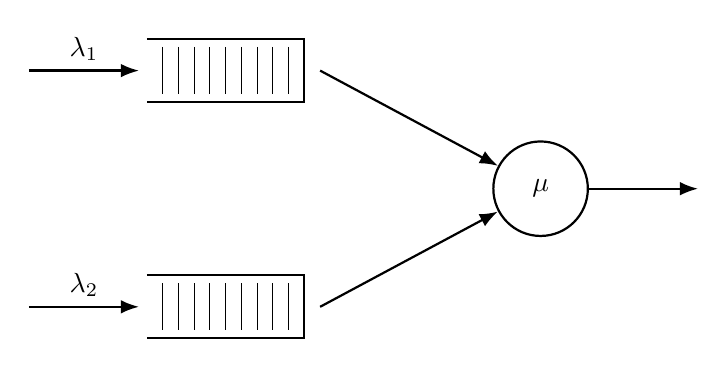
\begin{tikzpicture}[>=Latex, thick]

    % ── Queue 1 (top, Class-1, priority) ──────────────────────────────────────
    \draw (0, 1.9) -- (2, 1.9) -- (2, 1.1) -- (0, 1.1);
    \foreach \x in {0.2, 0.4, ..., 1.8} { \draw[thin] (\x, 1.8) -- (\x, 1.2); }
    \draw[->] (-1.5, 1.5) -- (-0.1, 1.5) node[midway, above] {$\lambda_1$};

    % ── Queue 2 (bottom, Class-2) ──────────────────────────────────────────────
    \draw (0, -1.1) -- (2, -1.1) -- (2, -1.9) -- (0, -1.9);
    \foreach \x in {0.2, 0.4, ..., 1.8} { \draw[thin] (\x, -1.2) -- (\x, -1.8); }
    \draw[->] (-1.5, -1.5) -- (-0.1, -1.5) node[midway, above] {$\lambda_2$};

    % ── Server ────────────────────────────────────────────────────────────────
    \node[draw, circle, minimum size=1.2cm] (server) at (5, 0) {$\mu$};
    \draw[->] (2.2,  1.5) -- (server);
    \draw[->] (2.2, -1.5) -- (server);
    \draw[->] (server) -- (7, 0);

\end{tikzpicture}
%
    }
    \caption{Queue layout for Model-$A$. Only Poisson arrivals and exponential service
    are present; all active mechanisms rates are zero.}
    \label{fig:model-a-queue}
\end{figure}

\subsection{Analysis of Model-\texorpdfstring{$A$}{A}: state space \texorpdfstring{$S$}{S}}
We begin from Equation~\eqref{eq:gen:fundamental_equation} with
$\gamma_1=\gamma_2=\theta_1=\theta_2=0$, in which the marginal $P_y(y)=P(0,y)$ is
still to be determined:
\begin{align}
    \begin{split}
        \left[ (\lambda_1+\lambda_2+ \mu)xy - \mu y - \lambda_1 x^2 y - \lambda_2 x y^2 \right] P(x,y)
         &= \mu(x-y) P_y(y)
         - \mu x(1-y) \pi(0,0).
    \end{split} \label{eq:A:fundamental}
\end{align}

The following theorem summarises the main result of this subsection; two standalone
proofs are given, one analytical and one probabilistic.
\begin{theorem}\label{thm:A:PGF}
    Consider a queueing system with two priority classes with Poisson arrival rates
    $\lambda_1$ and $\lambda_2$, where class-$1$ customers have non-preemptive priority
    over those of class~$2$, and exponentially distributed service times with rate $\mu$
    independently of the class. Under the stability condition $\rho<1$~\eqref{eq:A:stability}, the
    joint PGF $P(x,y) = \mathbb{E}[x^{N_1}y^{N_2}]$ is
    \begin{align}
        P(x,y) &= \left[ (1+\rho_1 +\rho_2)xy - y -\rho_1x^2y - \rho_2xy^2 \right]^{-1}
                  \cdot y(1-y) \left[ \frac{x - x^*(y)}{x^*(y)-y} \right] \cdot \rho (1-\rho),
        \label{eq:A:PGF}
    \end{align}
    where
    \begin{equation}
        x^*(y) = \frac{\left[\mu + \lambda_1 + \lambda_2 (1-y)\right]
                       - \sqrt{\left[\mu + \lambda_1 + \lambda_2 (1-y)\right]^2 - 4 \lambda_1 \mu}}
                      {2 \lambda_1}.
        \label{eq:A:xstar_def}
    \end{equation}
\end{theorem}

\begin{corollary}\label{cor:A:pi0}
    Under the stability condition $\rho < 1$~\eqref{eq:A:stability}, the empty-state probabilities
    for Model-$A$ are
    \begin{equation}
        \pi_0 = 1-\rho, \qquad \pi(0,0) = \rho(1-\rho). \label{eq:A:pi0_pi00}
    \end{equation}
    In particular, $P(1,1) = 1-\pi_0 = \rho$ and the diagonal generating function
    satisfies $P(z,z)=\pi(0,0)/(1-\rho z)$.
\end{corollary}

\begin{proof}[Proof of Corollary~\ref{cor:A:pi0}]
Setting $x=y=z$ in the fundamental equation~\eqref{eq:A:fundamental}, the boundary
term $\mu(x-y)P_y(y)$ vanishes:
    \begin{align*}
        \left[ (\lambda_1+\lambda_2+ \mu)z^2 - \mu z - \lambda_1 z^3 - \lambda_2 z^3 \right] P(z,z)
        &= - \mu z(1-z) \pi(0,0).
    \end{align*}
    Dividing both sides by $z$ and factoring the bracket:
    \begin{align*}
        -(1-z)\left[ \mu - (\lambda_1 + \lambda_2)z \right] P(z,z)
        &= - \mu (1-z) \pi(0,0).
    \end{align*}
    Cancelling $(1-z)\neq 0$ for $z\in[0,1)$ and rearranging:
    \begin{equation*}
        P(z,z) = \frac{\mu\,\pi(0,0)}{\mu - \lambda z} = \frac{\pi(0,0)}{1-\rho z},
    \end{equation*}
    where $\lambda = \lambda_1+\lambda_2$ and the second equality follows by dividing
    numerator and denominator by $\mu$.

    Setting $z=1$ and using the normalisation $P(1,1) = 1-\pi_0$:
    \begin{equation}
        1-\pi_0 = \frac{\pi(0,0)}{1-\rho}. \label{eq:A:norm_step}
    \end{equation}
    The global balance equation for the idle state gives $\lambda\pi_0 = \mu\pi(0,0)$,
    i.e.\ $\pi(0,0) = \rho\pi_0$. Substituting into~\eqref{eq:A:norm_step}:
    \begin{equation*}
        1-\pi_0 = \frac{\rho\pi_0}{1-\rho}
        \implies (1-\pi_0)(1-\rho) = \rho\pi_0
        \implies \pi_0 = 1-\rho,
    \end{equation*}
    and therefore $\pi(0,0) = \rho(1-\rho)$.
\end{proof}

\subsubsection{Analytical approach for Model-\texorpdfstring{$A$}{A} in state space \texorpdfstring{$S$}{S}}\label{sssec:A:analytical}

\begin{proof}[Proof of Theorem~\ref{thm:A:PGF}, analytical approach.]
    We begin from the fundamental equation for Model-$A$~\eqref{eq:A:fundamental}:
    \begin{equation*}
        \left[ (\lambda_1+\lambda_2+ \mu)xy - \mu y - \lambda_1 x^2y - \lambda_2 xy^2 \right] P(x,y)
        = \mu(x-y) P_y(y)  - \mu x(1-y) \pi(0,0).
    \end{equation*}
    We apply the \emph{Kernel Method}, used in ~\cite{cohen1956delay}: fix $y\in(0,1]$ and find $x^*(y)$ such that the LHS of the expression above is zero. Since $P(x,y)$ is a PGF, it is bounded. At any such root the LHS vanishes, so the RHS must also vanish:
    \[
        \mu\bigl[(x^*(y)-y)\,P_y(y) - x^*(y)(1-y)\,\pi(0,0)\bigr] = 0.
    \]
    To find the roots of the coefficient of $P(x,y)$, divide by $y\neq 0$ and set
    \begin{align*}
        \begin{split}
             0 &=  (\lambda_1 + \lambda_2 + \mu)x - \mu  -\lambda_1x^2 - \lambda_2xy
        \end{split} \\
        \begin{split}
          0 &=  \lambda_1 x^2 - \left[ \mu + \lambda_1 + \lambda_2 (1-y) \right] x + \mu,
        \end{split}
    \end{align*}
    whose roots are
    \begin{equation*}
        x^{\pm}(y) = \frac{
            \left[\mu + \lambda_1 + \lambda_2 (1-y) \right] \pm \sqrt{
                \left[\mu + \lambda_1 + \lambda_2 (1-y) \right]^2 - 4  \mu \lambda_1
            }
        }{
            2\lambda_1
        }.
    \end{equation*}
    
    We label the root with the negative sign $x^*(y)$ and the root with the positive
    sign $x^+(y)$. At $y=1$:
    \begin{equation*}
        x^*(1) = 1 \quad \text{and} \quad x^+(1) = \mu/\lambda_1 > 1.
    \end{equation*}
    
    We require our root to lie inside the closed unit disk for $y\in[0,1)$. Computing
    the derivative of $x^*(y)$:
    \begin{equation}
        \frac{d}{dy}x^*(y) = \frac{\lambda_2}{2\lambda_1}\!\left[-1+\frac{\mu+\lambda_1+\lambda_2(1-y)}{\sqrt{(\mu+\lambda_1+\lambda_2(1-y))^2-4\lambda_1\mu}}\right]>0,
        \label{eq:A:xstar_prime}
    \end{equation}
    since $(\mu+\lambda_1+\lambda_2(1-y))^2>(\mu+\lambda_1+\lambda_2(1-y))^2-4\lambda_1\mu$
    whenever $\lambda_1\mu>0$, by squaring numerator and denominator in the inner fraction. So $x^*(y)$ is strictly increasing in $[0,1]$, and since $x^*(1)=1$ we have $x^*(y)<1$ for $y\in[0,1)$.
    We make use of Vieta's formulas to discard the other root for the kernel polynomial
    $\lambda_1 x^2-[\mu+\lambda_1+\lambda_2(1-y)]x+\mu=0$: the product of the two
    roots satisfies $x^*(y)\,x^+(y)= \mu/\lambda_1>1$, so
    $x^+(y)=\mu/(\lambda_1 x^*(y))>1$ throughout $[0,1)$. So the only root
    strictly inside the unit disk for $y\in[0,1)$ is $x^*(y)$:
    \begin{equation}
        x^*(y) = \frac{
            (\mu +\lambda_1 + \lambda_2 (1-y))
            - \sqrt{(\mu +\lambda_1 + \lambda_2 (1-y))^2 - 4 \lambda_1 \mu}
        }{
            2\lambda_1
        }.
        \label{eq:A:xstar}
    \end{equation}

    Returning to the fundamental equation~\eqref{eq:A:fundamental} at $x=x^*(y)$,
    the RHS also equals zero, giving
    \begin{equation}
      \mu\cdot\left[(x^*(y)-y)P_y(y) - x^*(y)(1-y)\pi(0,0) \right]=0 \quad \implies \quad  P_y(y) = \frac{x^*(y)(1-y)}{x^*(y) - y} \pi(0,0). \label{eq:A:Py}
    \end{equation}

    By Corollary~\ref{cor:A:pi0}, $\pi(0,0)=\rho(1-\rho)$. Substituting this and
    Equation~\eqref{eq:A:Py} into the fundamental equation~\eqref{eq:A:fundamental}:
    \begin{align*}
        \begin{split}
            \left[ (\lambda_1+\lambda_2+ \mu)xy - \mu y - \lambda_1 x^2y - \lambda_2 xy^2 \right] P(x,y)
            &= \mu(x-y) \frac{x^*(y)(1-y)}{x^*(y) - y} \rho(1-\rho)  - \mu x(1-y) \rho(1-\rho)
        \end{split} \\
        \begin{split}
            \left[ (\lambda_1+\lambda_2+\mu)xy -\mu y-\lambda_1 x^2y - \lambda_2 xy^2 \right] P(x,y)
            &= \mu (1-y) \left[ \frac{x^*(y)(x-y)}{x^*(y)-y} - x \right] \rho (1-\rho)
        \end{split} \\
        \begin{split}
            \left[ (\lambda_1+\lambda_2+\mu)xy -\mu y-\lambda_1 x^2y - \lambda_2 xy^2 \right] P(x,y)
            &= \mu  (1-y) \left[ \frac{y(x - x^*(y))}{x^*(y) - y} \right] \rho (1-\rho)
        \end{split} \\
        \begin{split}
            \left[ (1 + \rho_1 + \rho_2)xy - y-\rho_1 x^2y - \rho_2 xy^2 \right] P(x,y)
            &= y (1-y) \left[ \frac{x - x^*(y)}{x^*(y) - y} \right] \rho (1-\rho).
        \end{split}
    \end{align*}

    Multiplying both sides by $\left[(1 + \rho_1 + \rho_2)xy - y-\rho_1 x^2y - \rho_2 xy^2\right]^{-1}$
    recovers $P(x,y)$ in Theorem~\ref{thm:A:PGF} and concludes the proof.
\end{proof}


\subsubsection{Probabilistic approach for Model-\texorpdfstring{$A$}{A} in state space \texorpdfstring{$S$}{S}}\label{sssec:A:probabilistic}
\begin{proof}[Proof of Theorem~\ref{thm:A:PGF}, probabilistic approach.]
    This proof mirrors the analytical one, but derives the class-$2$ marginal PGF $P_y(y)$ by means of probabilistic arguments. We again begin from the fundamental equation for Model-$A$ (Equation~\eqref{eq:A:fundamental}):
    \begin{equation}
        \left[ (\lambda_1 + \lambda_2 + \mu) xy - \mu y - \lambda_1 x^2 y - \lambda_2 x y^2 \right] P(x,y) =
        \mu \big[ (x-y) P_y(y) - x(1-y) \pi(0,0) \big].
        \label{eq:A:prob_starting}
    \end{equation}

    \paragraph{Class-$2$ conditional distribution via $M/G/1$.}
    Since class~$1$ has non-preemptive priority, class-$2$ customers are not taken into service
    whenever the priority queue is not empty ($N_1>0$); their \emph{effective service time} $B$ is therefore the duration of a complete busy period of the single-class ordinary $M/M/1$ sub-queue with arrival rate $\lambda_1$ and service rate $\mu$. From class-$2$'s viewpoint the system is thus an $M/G/1$ queue with arrival rate $\lambda_2$ and generally distributed service times $B$ and mean $\mathbb{E}[B]$. The LST and mean of $B$ are presented
    in~\S\ref{ssec:mm1} (Equations~\eqref{eq:mm1:bp_lst}--\eqref{eq:mm1:bp_mean}), now
    with $\lambda_1$ instead of the generic $\lambda$:
    \begin{align*}
        \widetilde{B}(s) &= \frac{(\mu+\lambda_1+s) - \sqrt{(\mu + \lambda_1 + s)^2-4\mu\lambda_1}}{2\lambda_1}, \\
        \mathbb{E}[B] &= \frac{1}{\mu(1-\rho_1)}. 
    \end{align*}
    Applying the Pollaczek--Khinchine (PK) formula (\S\ref{ssec:pk},
    Equation~\eqref{eq:pk:pgf}) to this $M/G/1$ system, with
    $\widetilde{B}(\lambda_2(1-y))=x^*(y)$ (cf.~\eqref{eq:A:xstar}) and
    $\lambda_2\mathbb{E}[B]=\rho_2/(1-\rho_1)$:
    \begin{align*}
        \begin{split}
            L_2(y) = \frac{(1 - \lambda_2 \mathbb{E}[B]) (1-y) \widetilde{B}(\lambda_2(1-y))}{\widetilde{B}(\lambda_2(1-y)) - y}
                    = \frac{1-\rho}{1-\rho_1} \cdot \frac{x^*(y)(1-y)}{x^*(y) - y}.
        \end{split}
    \end{align*}
    By the PASTA property, the time-average distribution of $N_2$ conditional on
    $(\text{busy},N_1=0)$ coincides with the $M/G/1$ steady-state distribution, so
    $\mathbb{E}[y^{N_2}\mid\text{busy},N_1=0]=L_2(y)$.

    By the law of total expectation, $P_y(y)=\mathbb{P}(\text{busy},N_1=0)\cdot\mathbb{E}[y^{N_2}\mid\text{busy},N_1=0]$. So
    \begin{equation*}
        P_y(y)=\mathbb{P}(\text{busy},N_1=0)\cdot\mathbb{E}[y^{N_2}\mid\text{busy},N_1=0] = \mathbb{P}(\text{busy},N_1=0)\cdot L_2(y).
    \end{equation*}
    Under non-preemptive priority, the priority queue operates autonomously (memorylessness of residual service time), so $\mathbb{P}(N_1=0 \mid \text{busy})=1-\rho_1$ by the geometric law of the ordinary $M/M/1(\lambda_1,\mu)$. Combined with $\mathbb{P}(\text{busy})=\rho$, we have
    \begin{equation*}
        \mathbb{P}(\text{busy},N_1=0)=\rho(1-\rho_1);
    \end{equation*}
    and therefore
    \begin{equation}
        P_y(y) = \rho(1-\rho_1)\cdot L_2(y) = \rho(1-\rho_1)\cdot\frac{1-\rho}{1-\rho_1} \cdot \frac{x^*(y)(1-y)}{x^*(y) - y} = \frac{x^*(y)(1-y)}{x^*(y) - y} \cdot (1-\rho) \rho
        \label{eq:A:Py_prob}
    \end{equation}

    Substituting~\eqref{eq:A:Py_prob} and $\pi(0,0)=\rho(1-\rho)$ (Corollary~\ref{cor:A:pi0})
    into~\eqref{eq:A:prob_starting}:
    \begin{align*}
        \begin{split}
            \left[ (\lambda_1+\lambda_2+\mu)xy - \mu y - \lambda_1 x^2y - \lambda_2 xy^2 \right] P(x,y)
            &= \mu(x-y) \frac{x^*(y)(1-y)}{x^*(y)-y} \rho(1-\rho) - \mu x(1-y) \rho(1-\rho)
        \end{split} \\
        \begin{split}
            \left[ (\lambda_1+\lambda_2+\mu)xy - \mu y - \lambda_1 x^2y - \lambda_2 xy^2 \right] P(x,y)&= \mu(1-y) \left[ \frac{x^*(y)(x-y)}{x^*(y)-y} - x \right] \rho(1-\rho)
        \end{split} \\
        \begin{split}
            \left[ (\lambda_1+\lambda_2+\mu)xy - \mu y - \lambda_1 x^2y - \lambda_2 xy^2 \right] P(x,y)&= \mu(1-y) \left[ \frac{y(x-x^*(y))}{x^*(y)-y} \right] \rho(1-\rho)
        \end{split} \\
        \begin{split}
            \left[ (1+\rho_1+\rho_2)xy - y - \rho_1 x^2y - \rho_2 xy^2 \right] P(x,y)
            &= y(1-y) \left[ \frac{x-x^*(y)}{x^*(y)-y} \right] \rho(1-\rho).
        \end{split}
    \end{align*}
    Multiplying both sides by $\left[ (1+\rho_1+\rho_2)xy - y - \rho_1 x^2y - \rho_2 xy^2 \right]^{-1}$
    to isolate $P(x,y)$ recovers Theorem~\ref{thm:A:PGF} and concludes the proof.
\end{proof}


\subsubsection{Partial-PGF recurrence approach for Model-\texorpdfstring{$A$}{A} in state space \texorpdfstring{$S$}{S}}


This proof follows Cohen~\cite{cohen1956delay}'s method. We keep the class-$1$
index $n_1$ as a discrete parameter and generate only with respect
to $N_2$, via the PPGF $\widetilde{P}(n_1,y)=\sum_{n_2\geq0}\pi(n_1,n_2)\,y^{n_2}$
from~\eqref{eq:gen:ppgf_n1}. Multiplying the balance equations by $y^{n_2}$ and
summing over $n_2$ turns them into a second-order linear
recurrence in $n_1$, whose characteristic roots fix the geometric structure of the
solution in the priority-class index.

\begin{proof}
    We start from the Model-$A$ balance equations, obtained by setting $\gamma_1=\gamma_2=\theta_1=\theta_2=0$ in the interior equation~\eqref{eq:gen:balance_interior} and the $x$-boundary equation~\eqref{eq:gen:balance_x_boundary}:
    \begin{align}
        (\lambda_1+\lambda_2+\mu)\,\pi(n_1,n_2)
            &= \mu\,\pi(n_1+1,n_2) + \lambda_1\,\pi(n_1-1,n_2) + \lambda_2\,\pi(n_1,n_2-1),
            && n_1\geq1,\ n_2\geq1, \nonumber\\
        (\lambda_1+\lambda_2+\mu)\,\pi(n_1,0)
            &= \mu\,\pi(n_1+1,0) + \lambda_1\,\pi(n_1-1,0),
            && n_1\geq1,\ n_2=0. \label{eq:A:ppgf_xbound}
    \end{align}
    Now we take transforms by summing all over their states, but only with respect to $n_2$, and we substitute our PPGF $\widetilde{P}(n_1,y)=\sum_{n_2=0}^{\infty} \pi(n_1,y)y^{n_2}$:
    \begin{align}
        \begin{split}
            & (\lambda_1+\lambda_2+\mu)\sum_{n_2=1}^{\infty}\pi(n_1,n_2)y^{n_2} \\
            & \quad = \quad \mu\sum_{n_2=1}^{\infty}\pi(n_1+1,n_2)y^{n_2} + \lambda_1\sum_{n_2=1}^{\infty}\pi(n_1-1,n_2)y^{n_2} + \lambda_2\sum_{n_2=1}^{\infty}\pi(n_1,n_2-1)y^{n_2}
        \end{split} \nonumber \\
        \begin{split}
            & LHS_1 \quad = \quad RHS_1 + RHS_2 + RHS_3
        \end{split} \nonumber \\
        \begin{split}
            & LHS_1 \\
            & \quad = \quad (\lambda_1+\lambda_2+\mu)\sum_{n_2=1}^{\infty}\pi(n_1,n_2)y^{n_2} \\
            & \quad = \quad (\lambda_1+\lambda_2+\mu) \left[ \sum_{n_2=0}^{\infty}\pi(n_1,n_2)y^{n_2} - \pi(n_1,0)y^0 \right] \\
            & \quad = \quad (\lambda_1+\lambda_2+\mu) \left[ \widetilde{P}(n_1,y) - \pi(n_1,0) \right]
        \end{split} \nonumber \\
        \begin{split}
            & RHS_1 \\
            & \quad = \quad \mu\sum_{n_2=1}^{\infty}\pi(n_1+1,n_2)y^{n_2} \\
            & \quad = \quad \mu \left[ \sum_{n_2=0}^{\infty}\pi(n_1+1,n_2)y^{n_2} - \pi(n_1+1,0)y^0 \right] \\
            & \quad = \quad \mu \left[ \widetilde{P}(n_1+1,y) - \pi(n_1+1,0) \right]
        \end{split} \nonumber \\
        \begin{split}
            & RHS_2 \\
            & \quad = \quad \lambda_1\sum_{n_2=1}^{\infty}\pi(n_1-1,n_2)y^{n_2} \\
            & \quad = \quad \lambda_1 \left[ \sum_{n_2=0}^{\infty}\pi(n_1-1,n_2)y^{n_2} - \pi(n_1-1,0)y^0 \right] \\
            & \quad = \quad \lambda_1 \left[ \widetilde{P}(n_1-1,y) - \pi(n_1-1,0) \right]
        \end{split} \nonumber \\
        \begin{split}
            & RHS_3 \\
            & \quad = \quad \lambda_2\sum_{n_2=1}^{\infty}\pi(n_1,n_2-1)y^{n_2} \\
            & \quad = \quad \lambda_2 y \sum_{n_2=1}^{\infty}\pi(n_1,n_2-1)y^{n_2-1} \\
            & \quad = \quad \lambda_2 y \sum_{m=0}^{\infty}\pi(n_1,m)y^{m} \\
            & \quad = \quad \lambda_2 y \, \widetilde{P}(n_1,y)
        \end{split} \nonumber \\
        \begin{split}
            & (\lambda_1+\lambda_2+\mu)\bigl[\widetilde{P}(n_1,y)-\pi(n_1,0)\bigr] \\
            & \quad = \quad \mu\bigl[\widetilde{P}(n_1+1,y)-\pi(n_1+1,0)\bigr] \\
            & \quad \quad + \; \lambda_1\bigl[\widetilde{P}(n_1-1,y)-\pi(n_1-1,0)\bigr] \\
            & \quad \quad + \; \lambda_2 y\,\widetilde{P}(n_1,y)
        \end{split} \nonumber \\
        \begin{split}
            & \bigl[\mu+\lambda_1+\lambda_2(1-y)\bigr]\widetilde{P}(n_1,y) -\mu\widetilde{P}(n_1+1,y)-\lambda_1\widetilde{P}(n_1-1,y) \\
            & \quad = \quad (\lambda_1+\lambda_2+\mu)\pi(n_1,0) -\mu\pi(n_1+1,0)-\lambda_1\pi(n_1-1,0)
        \end{split}
        \label{eq:A:ppgf_final_boundary}
    \end{align}
    By the $x$-boundary balance equation~\eqref{eq:A:ppgf_xbound}, the right-hand side of~\eqref{eq:A:ppgf_final_boundary} vanishes completely, giving the homogeneous recurrence
    \begin{equation}
        \left[ \mu + \lambda_1 + \lambda_2 (1-y) \right] \widetilde{P}(n_1,y)
        = \mu \widetilde{P}(n_1+1,y)
        + \lambda_1 \widetilde{P}(n_1-1,y),
        \qquad n_1\geq1.
        \label{eq:A:ppgf_recurrence}
    \end{equation}
    
    \paragraph{Characteristic roots and mode selection.}
    Equation~\eqref{eq:A:ppgf_recurrence} is a \emph{second-order linear recurrence} in $n_1$ with constant coefficients, so its general solution is a linear combination of two geometric sequences $[\widetilde{x}^{\pm}(y)]^{n_1}$, where $\widetilde{x}^{\pm}(y)$ solve the characteristic equation
    \begin{equation}
        \mu\,\widetilde{x}^2 - \left[ \mu + \lambda_1 + \lambda_2(1-y) \right]\widetilde{x} + \lambda_1 = 0,
        \label{eq:A:ppgf_char}
    \end{equation}
    that is,
    \begin{equation*}
        \widetilde{x}^{\pm}(y)
        = \frac{\bigl(\mu + \lambda_1 + \lambda_2(1-y)\bigr)
                \pm \sqrt{\bigl(\mu + \lambda_1 + \lambda_2(1-y)\bigr)^2 - 4\lambda_1\mu}}{2\mu}.
    \end{equation*}
    The \emph{characteristic polynomial} (Equation \eqref{eq:A:ppgf_char}) is the reciprocal to that of the bivariate PGF approaches (i.e. the reciprocal of $\lambda_1 x^2-[\mu+\lambda_1+\lambda_2(1-y)]x+\mu$), thus its roots are the reciprocals of that kernel's roots: the positive root is the reciprocal of the negative one ($\widetilde{x}^{+}(y)=1/x^*(y)$), and conversely $\widetilde{x}^{-}(y)=1/x^{+}(y)$. By Vieta's formulas, $\widetilde{x}^{-}(y)\,\widetilde{x}^{+}(y)=\lambda_1/\mu=\rho_1<1$. Recall from \S\ref{sssec:A:analytical} that $x^*(y)<1<x^{+}(y)$ for $y\in[0,1)$.
    We select the negative-sign root because the sequence $\{\widetilde{P}(n_1,y)\}_{n_1\geq0}$ must be summable:
    \begin{equation*}
        \sum_{n_1=0}^{\infty}\widetilde{P}(n_1,y) = P(1,y) \le P(1,1) = 1-\pi_0 = \rho < \infty.
    \end{equation*}
    At $y=1$, we have
    \begin{equation*}
        \widetilde{x}^{-}(1)=\rho_1 \quad \text{and} \quad \widetilde{x}^{+}(1)=1,
    \end{equation*}
    the latter making the geometric sequence $[\widetilde{x}^{+}(y)]^{n_1}$ non-summable. We therefore define $\widetilde{x}^*(y):=\widetilde{x}^{-}(y)$,
    \begin{equation}
        \widetilde{x}^*(y):=\widetilde{x}^{-}(y) = \frac{\bigl(\mu + \lambda_1 + \lambda_2(1-y)\bigr)
                - \sqrt{\bigl(\mu + \lambda_1 + \lambda_2(1-y)\bigr)^2 - 4\lambda_1\mu}}{2\mu}
        = \rho_1\,x^*(y).
        \label{eq:A:xtildestar}
    \end{equation}
    The last identity holds because $\widetilde{x}^*$ and $x^*$ share the same numerator and differ only in the denominator ($2\mu$ versus $2\lambda_1$). Next,
    \begin{equation}
        \widetilde{P}(n_1, y) = \widetilde{P}(0,y)\,[\widetilde{x}^*(y)]^{n_1},
        \qquad n_1\geq0,
        \label{eq:A:ppgf_geometric}
    \end{equation}
    where the relation also holds at $n_1=0$ trivially.
    Recall that at $y=1$, we have $\widetilde{x}^*(1)=\lambda_1/\mu=\rho_1$. Thus, $\widetilde{P}(n_1,1)=\widetilde{P}(0,1)\,\rho_1^{n_1}$ and $\widetilde{P}(0,1)=P_y(1)=\rho(1-\rho_1)$. The constant $\widetilde{P}(0,y)$ is resolved by its definition
    \begin{equation*}
        \widetilde{P}(0,y) = \sum_{n_2=0}^{\infty}\pi(0,n_2)\,y^{n_2} = P(0,y) = P_y(y),
    \end{equation*}
    as determined in the bivariate PGF approaches.
    Summing the geometric law (Equation~\eqref{eq:A:ppgf_geometric}) over $n_1 \geq 0$ for $x \in (0,1]$ recovers
    \begin{equation}
        P(x,y) = \sum_{n_1=0}^{\infty}\widetilde{P}(n_1,y)\,x^{n_1}
               = P_y(y)\sum_{n_1=0}^{\infty}\bigl[\widetilde{x}^*(y)\,x\bigr]^{n_1}
               = \frac{P_y(y)}{1-\widetilde{x}^*(y)\,x}.
        \label{eq:A:ppgf_reconstruct}
    \end{equation}
    To bring this to the form of Theorem~\ref{thm:A:PGF}, we define the kernel of the fundamental equation, divided by $\mu$:
    \begin{equation}
        K(x,y) := (1+\rho_1+\rho_2)xy - y - \rho_1 x^2 y - \rho_2 x y^2
                = -y\rho_1\bigl(x-x^*(y)\bigr)\bigl(x-x^{+}(y)\bigr),
        \label{eq:A:kernel_factored}
    \end{equation}
    where $x^*(y)$ and $x^{+}(y)$ are the roots found in \S\ref{sssec:A:analytical}. By Vieta's product formula, $x^*(y)\,x^{+}(y)=\mu/\lambda_1=1/\rho_1$. This, together with $\widetilde{x}^*(y)$ (Equation \eqref{eq:A:xtildestar}), gives $\widetilde{x}^*(y)=\rho_1 x^*(y)=1/x^{+}(y)$.
    Using the factorisation of $K(x,y)$~\eqref{eq:A:kernel_factored}, the denominator of the reconstructed PGF~\eqref{eq:A:ppgf_reconstruct} becomes
    \begin{equation*}
        1-\widetilde{x}^*(y)\,x = 1 - \frac{x}{x^{+}(y)} = \frac{x^{+}(y)-x}{x^{+}(y)}
        = \frac{K(x,y)}{y\rho_1\,x^{+}(y)\bigl(x-x^*(y)\bigr)}.
    \end{equation*}
    Substituting this into our reconstructed $P(x,y)$ (Equation \eqref{eq:A:ppgf_reconstruct}), using 
    $P_y(y)=\frac{x^*(y)(1-y)}{x^*(y)-y}\rho(1-\rho)$ and also noting that $\rho_1\,x^*(y)\,x^{+}(y)=1$, we obtain
    \begin{align*}
        P(x,y)
        &= \frac{x^*(y)(1-y)}{x^*(y)-y}\,\rho(1-\rho)
           \cdot \frac{y\rho_1\,x^{+}(y)\bigl(x-x^*(y)\bigr)}{K(x,y)} \\
        &= \underbrace{\rho_1\,x^*(y)\,x^{+}(y)}_{=\,1}\;
           \frac{1}{K(x,y)}\, y(1-y)\,\frac{x-x^*(y)}{x^*(y)-y}\,\rho(1-\rho) \\
        &= \bigl[(1+\rho_1+\rho_2)xy - y - \rho_1 x^2 y - \rho_2 x y^2\bigr]^{-1}
           \cdot y(1-y)\,\frac{x-x^*(y)}{x^*(y)-y}\,\rho(1-\rho),
    \end{align*}
    which recovers Equation~\eqref{eq:A:PGF} from Theorem~\ref{thm:A:PGF} and concludes the proof.
\end{proof}


\subsection{Analysis of Model-\texorpdfstring{$A$}{A} on \texorpdfstring{$\widetilde{S}$}{S~}: scope and limitations of the partial-PGF recursion}\label{ssec:A:Stilde}

Setting $\gamma_1=\gamma_2=\theta_1=\theta_2=0$ in the $\widetilde{S}$ balance
equations~\eqref{eq:gen:tilde_balance_interior}--\eqref{eq:gen:tilde_balance_idle}
and forming the PPGF $\widetilde{P}(y,n)=\sum_{n_2=0}^n \widetilde{\pi}(n_2,n)\,y^{n_2}$
yields the inhomogeneous recurrence:
\begin{align}
    \begin{split}
       &\left[ \lambda_1 + \lambda_2 + \mu \right] \widetilde{P}(y,n) \\
       & \quad = \quad(\lambda_1 + \lambda_2 y) \widetilde{P}(y,n-1) + \mu \widetilde{P}(y,n+1)
                  + \mu y^n (1-y) \tpi(n+1,n+1)
    \end{split} \label{eq:A:ppgf_Stilde_dynamics}
\end{align}

The forcing term in~\eqref{eq:A:ppgf_Stilde_dynamics} is controlled by the diagonal
probabilities $\tpi(n+1,n+1)=\pi(0,n+1)$, whose decay we first establish from the exact
$S$-solution.

\begin{lemma}[Geometric decay of the boundary probabilities]\label{lem:A:diag_decay}
    For Model-$A$ the boundary probabilities $\pi(0,n)$ satisfy $\pi(0,n)=O(r^{-n})$ for
    every $r<1/\rho$; equivalently they decay geometrically with rate $\rho$.
\end{lemma}

\begin{proof}
    By definition $P_y(y)=P(0,y)=\sum_{n\ge0}\pi(0,n)\,y^n$ is the generating function of
    $\{\pi(0,n)\}$, and from~\eqref{eq:A:Py} with $\pi(0,0)=\rho(1-\rho)$,
    \begin{equation*}
        P_y(y)=\rho(1-\rho)\,\frac{x^*(y)(1-y)}{x^*(y)-y}.
    \end{equation*}
    Evaluating the kernel quadratic~\eqref{eq:A:xstar_def} at $x=y$ gives
    $\lambda_1 y^2-[\mu+\lambda_1+\lambda_2(1-y)]y+\mu=(\lambda y-\mu)(y-1)$ with
    $\lambda=\lambda_1+\lambda_2$, so $x^*(y)=y$ holds only at $y=1$ and $y=\mu/\lambda=1/\rho$.
    At $y=1$ the simple zeros of $(1-y)$ and $(x^*(y)-y)$ cancel and $P_y$ is analytic with
    $P_y(1)=\rho$; the branch point of $x^*$ lies beyond $1/\rho$. Hence the singularity of
    $P_y$ nearest the origin is the simple pole at $y=1/\rho>1$, so $P_y$ is analytic on the
    disc $|y|<1/\rho$. By the Cauchy coefficient estimates, for every $r<1/\rho$ there is
    $C_r<\infty$ with $\pi(0,n)\le C_r\,r^{-n}$, i.e.\ geometric decay at rate $\rho$.
\end{proof}

\begin{approximation}[Heuristic PPGF on $\widetilde{S}$]\label{apx:A:PPGF_Stilde}
    Neglecting the boundary-diagonal forcing term
    $\mu y^n(1-y)\,\tpi(n+1,n+1)$ in~\eqref{eq:A:ppgf_Stilde_dynamics} --- which is
    exponentially small by Lemma~\ref{lem:A:diag_decay} --- the
    homogeneous recurrence admits the geometric solution
    \begin{equation*}
        \widetilde{P}(y,n) \;\approx\; \rho(1-\rho)\,[\widetilde{y}^*(y)]^n, 
    \end{equation*}
    where
    \begin{equation*}
        \widetilde{y}^*(y) = \frac{(\lambda+\mu) - \sqrt{(\lambda+\mu)^2 - 4\mu(\lambda_1+\lambda_2 y)}}{2\mu}, \qquad \lambda = \lambda_1+\lambda_2. 
    \end{equation*}
    At $y=1$ this recovers $\widetilde{P}(1,n)=(1-\rho)\rho^{n+1}$, consistent with
    the $M/M/1(\lambda,\mu)$ steady-state marginal for $n$ customers waiting.
\end{approximation}

\begin{proof}[Justification of Approximation~\ref{apx:A:PPGF_Stilde}]
The inhomogeneous term $\mu y^n(1-y)\tpi(n+1,n+1)$ prevents the direct application
of a geometric-sequence ansatz. The diagonal probabilities $\tpi(n,n)=\pi(0,n)$
correspond to states where all $n$ waiting customers are class~$2$, and by
Lemma~\ref{lem:A:diag_decay} they decay geometrically in $n$ at rate $\rho$; the
forcing term is therefore exponentially small, and neglecting it yields an
approximation whose accuracy is quantified below. The resulting homogeneous recurrence is
\begin{equation*}
    (\lambda_1 + \lambda_2 + \mu) \widetilde{P}(y,n) = (\lambda_1 + \lambda_2 y) \widetilde{P}(y,n-1) + \mu \widetilde{P}(y,n+1).
\end{equation*}
The characteristic polynomial of this recurrence is
\begin{equation*}
    \mu [\widetilde{y}(y)]^2 - (\lambda_1 + \lambda_2 + \mu) \widetilde{y}(y) + (\lambda_1 + \lambda_2 y) = 0,
\end{equation*}
with roots
\begin{equation*}
    \widetilde{y}^{\pm}(y) = \frac{(\lambda_1 + \lambda_2 + \mu) \pm \sqrt{(\lambda_1 + \lambda_2 + \mu)^2 - 4\mu(\lambda_1 + \lambda_2 y)}}{2\mu}.
\end{equation*}
At $y=1$ the roots are $\widetilde{y}_{+}(1)=1$ and $\widetilde{y}_{-}(1)=\rho$.
The root $\widetilde{y}_{+}=1$ would produce a non-summable geometric series as
$n\to\infty$, so only the negative-sign root is admissible:
\begin{equation*}
    \widetilde{y}^*(y) = \frac{(\lambda_1 + \lambda_2 + \mu) - \sqrt{(\lambda_1 + \lambda_2 + \mu)^2 - 4\mu(\lambda_1 + \lambda_2 y)}}{2\mu}.
\end{equation*}
The geometric ansatz gives $\tP(y,n)=\tP(y,0) \cdot [\widetilde{y}^*(y)]^n$.
Using $\tP(y,0)=\tpi(0,0)=\pi(0,0)=\rho(1-\rho)$ (Corollary~\ref{cor:A:pi0}):
\begin{equation*}
    \tP(y,n)=\rho(1-\rho) \cdot  [\widetilde{y}^*(y)]^n.
\end{equation*}
Since $n$ counts customers \emph{waiting} (the customer in service is not counted),
$n+1$ is the total number in the system, so evaluating at $y=1$:
\begin{equation*}
    \tP(1,n)= \rho(1-\rho) \cdot\rho^n= (1-\rho) \rho^{n+1}, \qedhere
\end{equation*}
which matches the $M/M/1(\lambda,\mu)$ stationary distribution for $n+1$ customers
in the system~\cite{adan2002queueing}.
\end{proof}

\paragraph{Failure mechanism.}
The neglected forcing $\mu y^n(1-y)\,\tpi(n+1,n+1)$ feeds in the diagonal states, in which
all waiting customers are class~$2$. Using $\tpi(n,n)=\pi(0,n)$ and the rate proved
in Lemma~\ref{lem:A:diag_decay}, this term decays in $n$ like $\rho^{\,n}$ (modulated by
$y^n$), whereas the homogeneous solution decays like $[\widetilde{y}^*(y)]^n$. The
approximation is therefore accurate exactly when the forcing decays faster, i.e.\
$\rho<\widetilde{y}^*(y)$ on the relevant range of $y$; this holds when the priority
class carries most of the load ($\rho_1/\rho$ large, $\rho$ moderate), precisely the
empirical validity region of the approximation.

The obstruction is structural and recurs throughout this thesis: an unknown boundary/diagonal
trace --- here the sequence $\pi(0,n)$ --- couples into an otherwise solvable recursion,
exactly as the unknown diagonal $P(z,z)$ enters the Volterra forcing of Models~$B$ and~$X$
(\S\ref{sec:model_b} and Remark~\ref{rem:B:modelX}). A rigorous closure would retain the forcing
and solve~\eqref{eq:A:ppgf_Stilde_dynamics} by variation of constants in $n$, which
reintroduces the very diagonal sequence $\{\pi(0,n)\}$ as an unknown to be determined
self-consistently; see \S\ref{sec:future_work}.

\section{Analysis of Model-\texorpdfstring{$B$}{B} (\texorpdfstring{$\gamma_1,\gamma_2>0$}{gamma1,gamma2>0}, \texorpdfstring{$\theta_1=\theta_2=0$}{theta1=theta2=0})}\label{sec:model_b}

Model-$B$ introduces bidirectional jockeying ($\gamma_1,\gamma_2>0$) while retaining no abandonment ($\theta_1=\theta_2=0$). Jockeying conserves the total number of customers in the system, so the stationary distribution still exists under the same condition as Model-$A$. However, jockeying breaks the per-class Poisson/renewal structure: a class-2 customer can no longer identify its effective service time with a class-1 busy period, so the Pollaczek--Khinchine probabilistic route is unavailable. Applying the method of characteristics to the fundamental equation yields a general solution, but closing it~---~i.e., determining the unknown boundary function $P_y(y)$~---~requires solving a Volterra-type integral equation that does not admit a closed form. Model-$B$ is therefore intentionally left open, in structural parallel with Model-$X$; its role is to motivate the tractable specialisation Model-$B_2$.

\textbf{Stability.} $\rho = (\lambda_1+\lambda_2)/\mu < 1$. Jockeying conserves the total customer count and does not affect this condition. Figure~\ref{fig:model-b-queue} shows the queue layout.

\begin{figure}[H]
    \centering
    \resizebox{0.62\textwidth}{!}{%
        % Model B: θ₁=θ₂=0, γ₁,γ₂>0
% Bidirectional jockeying between queues (dashed). No abandonment.
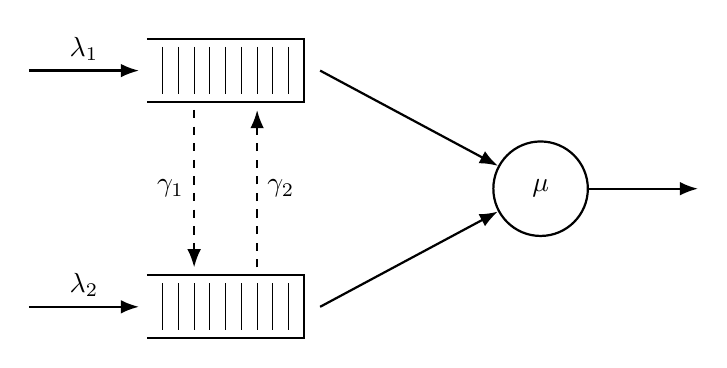
\begin{tikzpicture}[>=Latex, thick]

    % ── Queue 1 (top, Class-1, priority) ──────────────────────────────────────
    \draw (0, 1.9) -- (2, 1.9) -- (2, 1.1) -- (0, 1.1);
    \foreach \x in {0.2, 0.4, ..., 1.8} { \draw[thin] (\x, 1.8) -- (\x, 1.2); }
    \draw[->] (-1.5, 1.5) -- (-0.1, 1.5) node[midway, above] {$\lambda_1$};

    % ── Queue 2 (bottom, Class-2) ──────────────────────────────────────────────
    \draw (0, -1.1) -- (2, -1.1) -- (2, -1.9) -- (0, -1.9);
    \foreach \x in {0.2, 0.4, ..., 1.8} { \draw[thin] (\x, -1.2) -- (\x, -1.8); }
    \draw[->] (-1.5, -1.5) -- (-0.1, -1.5) node[midway, above] {$\lambda_2$};

    % ── Jockeying between queues ──────────────────────────────────────────────
    % γ₁: Class-1 jockeys down to Class-2 queue
    \draw[->, dashed] (0.6, 1.0) -- (0.6, -1.0) node[midway, left] {$\gamma_1$};
    % γ₂: Class-2 jockeys up to Class-1 queue
    \draw[->, dashed] (1.4, -1.0) -- (1.4, 1.0) node[midway, right] {$\gamma_2$};

    % ── Server ────────────────────────────────────────────────────────────────
    \node[draw, circle, minimum size=1.2cm] (server) at (5, 0) {$\mu$};
    \draw[->] (2.2,  1.5) -- (server);
    \draw[->] (2.2, -1.5) -- (server);
    \draw[->] (server) -- (7, 0);

\end{tikzpicture}
%
    }
    \caption{Queue layout for Model-$B$. Dashed arrows indicate bidirectional
    jockeying: $\gamma_1$ moves a class-1 customer down to Queue~2 and $\gamma_2$
    moves a class-2 customer up to Queue~1. Both transfers conserve the total~$n$.}
    \label{fig:model-b-queue}
\end{figure}

\begin{corollary}\label{cor:B:pi00}
    The empty-system probability $\pi_0$ (server idle, no one waiting) and the
    both-queues-empty probability $\pi(0,0)$ (server busy, $N_1=N_2=0$) of Model-$B$
    coincide with the Model-$A$ baseline,
    \begin{equation}
        \pi_0 = 1-\rho, \qquad \pi(0,0) = \rho(1-\rho),
        \label{eq:B:pi00}
    \end{equation}
    and the diagonal of the PGF is $P(z,z)=\pi(0,0)/(1-\rho z)$.
\end{corollary}

\begin{proof}
    Setting $x=y$ in the fundamental equation~\eqref{eq:gen:fundamental_equation} with
    $\theta_1=\theta_2=0$, both jockeying terms carry the factor $(x-y)$ and vanish, as
    does the boundary term $\mu(x-y)P_y(y)$; dividing the surviving terms by the common
    factor $x$ leaves
    \begin{equation*}
        \bigl[(\lambda_1+\lambda_2+\mu)x - \mu - (\lambda_1+\lambda_2)x^2\bigr]P(x,x)
        = -\mu(1-x)\,\pi(0,0).
    \end{equation*}
    Writing $\lambda=\lambda_1+\lambda_2$, the bracket factors,
    \begin{equation}
        (\lambda+\mu)x-\mu-\lambda x^{2}
        = -\bigl(\lambda x^{2}-(\lambda+\mu)x+\mu\bigr)
        = -(\lambda x-\mu)(x-1)
        = (\mu-\lambda x)(x-1);
        \nonumber
    \end{equation}
    cancelling $(x-1)$ against $-(1-x)=(x-1)$ on the right gives
    \begin{equation}
        P(x,x) = \frac{\mu\,\pi(0,0)}{\mu-\lambda x} = \frac{\pi(0,0)}{1-\rho x}.
        \label{eq:B:Pxx}
    \end{equation}
    The idle state $(0)$ exchanges probability flux only with the both-queues-empty busy
    state, so the global balance across the idle--busy cut reads
    $\lambda\pi_0=\mu\pi(0,0)$ (an arrival at total rate $\lambda$ leaves $(0)$; a service
    completion at rate $\mu$ returns to it), whence $\pi(0,0)=\rho\pi_0$. Evaluating
    \eqref{eq:B:Pxx} at $x=1$ with $P(1,1)=1-\pi_0$ gives
    $1-\pi_0=\rho\pi_0/(1-\rho)$, so $(1-\pi_0)(1-\rho)=\rho\pi_0$, i.e.\ $\pi_0=1-\rho$
    and $\pi(0,0)=\rho(1-\rho)$. This matches Model-$A$~\eqref{eq:A:pi0_pi00}: jockeying
    conserves the total-customer process and cannot change the marginal idle probability.
    The same identities hold in Models~$B_2$ and~$C_2$ for the same conservation
    reason~\eqref{eq:gen:pi0_noaband}.
\end{proof}

\begin{claim}\label{clm:B:volterra}
    Under stability, $\rho<1$, the bivariate PGF of Model-$B$ satisfies, on each
    characteristic curve $\gamma_2 x + \gamma_1 y = C_1$ of the fundamental equation,
    the integral representation
    \begin{equation}
        P(x,y(x)) \;=\; P_h(x,y(x))\int_{0}^{x}
        \frac{h\bigl(t;\,C_1\bigr)}{P_h\bigl(t,\,y(t)\bigr)}\,dt,
        \label{eq:B:integral_rep}
    \end{equation}
    where $P_h$ is the homogeneous solution~\eqref{eq:B:Ph}, $y(t)=(C_1-\gamma_2 t)/\gamma_1$
    is the characteristic parametrisation, and $h(t;C_1)$ is an explicit forcing
    function depending on the unknown boundary trace $P_y(y)=P(0,y)$.
    Evaluating~\eqref{eq:B:integral_rep} along the diagonal $x=y=z$ and using the
    conservation identity $P(z,z)=\pi(0,0)/(1-\rho z)$ reduces the problem to a
    \emph{Volterra integral equation of the first kind} for $P_y$:
    \begin{equation}
        \mathcal{F}(z) \;=\; \int_0^z \mathcal{K}(z,t)\,P_y\!\bigl(y(t;z)\bigr)\,dt,
        \label{eq:B:volterra}
    \end{equation}
    where $\mathcal{K}$ and $\mathcal{F}$ are fully explicit
    (defined in~\eqref{eq:B:kernel}--\eqref{eq:B:rhs} below). The kernel
    $\mathcal{K}$ does not factorise for general $(\gamma_1,\gamma_2)$,
    so~\eqref{eq:B:volterra} does not reduce to a closed-form solution for $P_y$.
    Model-$B$ is therefore left open.
\end{claim}

\begin{proof}[Proof of Claim~\ref{clm:B:volterra}]
The proof proceeds in five steps: (i)~homogeneous solution via characteristics,
(ii)~rigorous sign analysis of the exponent $E$, (iii)~particular solution via
variation of parameters, (iv)~pinning the free function from the boundary condition,
and (v)~diagonal evaluation yielding the Volterra equation.

% ─────────────────────────────────────────────────────────────────────────────
\medskip\noindent\textbf{Step~1: Homogeneous solution via the method of characteristics.}

The fundamental equation~\eqref{eq:gen:fundamental_equation} with
$\theta_1=\theta_2=0$ is a first-order linear PDE in $P(x,y)$. Setting the
right-hand side to zero and dividing through by $y$ yields the homogeneous PDE
\begin{equation*}
    \gamma_1 x(x-y)\,\frac{\partial P}{\partial x}
    - \gamma_2 x(x-y)\,\frac{\partial P}{\partial y}
    = -\bigl[(\lambda_1+\lambda_2+\mu)x - \mu - \lambda_1 x^2
             - \lambda_2 xy\bigr]P.
\end{equation*}
Following the method of characteristics (\S\ref{sssec:moc}), we associate to
this PDE the characteristic system
\begin{equation*}
    \frac{dx}{\gamma_1 x(x-y)}
    = \frac{dy}{-\gamma_2 x(x-y)}
    = \frac{dP}{-\bigl[(\lambda_1+\lambda_2+\mu)x - \mu
               - \lambda_1 x^2 - \lambda_2 xy\bigr]P}.
\end{equation*}
Taking the ratio of the first two differentials, the $x(x-y)$ factors cancel,
giving $dx/\gamma_1 = dy/(-\gamma_2)$.  Integrating yields the first integral
\begin{equation*}
    C_1 = \gamma_2 x + \gamma_1 y \quad\text{(constant along each characteristic)}.
\end{equation*}
The characteristics are therefore the straight lines of slope $-\gamma_2/\gamma_1$
in the $(x,y)$-plane. Fix one such line and parametrise $y$ by
$y(x) = (C_1-\gamma_2 x)/\gamma_1$.  To extract the equation for $P$ along this
curve we need the coefficient $A(x,y)$ and the denominator $x(x-y)$ after
substitution.  Setting
\begin{equation}
    A(x,y) := (\lambda_1+\lambda_2+\mu)x - \mu - \lambda_1 x^2 - \lambda_2 xy,
    \label{eq:B:Adef}
\end{equation}
and substituting $y = (C_1-\gamma_2 x)/\gamma_1$ so that
$\lambda_2 xy = (\lambda_2 C_1/\gamma_1)x - (\lambda_2\gamma_2/\gamma_1)x^2$,
we obtain, collecting by powers of $x$,
\begin{align*}
    \begin{split}
    A\bigl(x,y(x)\bigr)
    &= (\lambda_1+\lambda_2+\mu)x - \mu - \lambda_1 x^2
       - \frac{\lambda_2 C_1}{\gamma_1}\,x + \frac{\lambda_2\gamma_2}{\gamma_1}\,x^2 \\
    &= -\frac{\gamma_1\lambda_1-\lambda_2\gamma_2}{\gamma_1}\,x^2
       + \frac{\gamma_1(\lambda_1+\lambda_2+\mu)-\lambda_2 C_1}{\gamma_1}\,x
       - \mu.
    \end{split}
\end{align*}
Similarly, $x - y(x) = [(\gamma_1+\gamma_2)x-C_1]/\gamma_1$, so
$\gamma_1 x(x-y(x)) = x[(\gamma_1+\gamma_2)x-C_1]$.  The $dP/P$ equation from
the characteristic system therefore becomes
\begin{align*}
    \frac{dP}{P}
    &= \frac{-A(x,y(x))}{\gamma_1 x(x-y(x))}\,dx
     = \frac{(\gamma_1\lambda_1 - \lambda_2\gamma_2)x^2
             - \bigl[\gamma_1(\lambda_1+\lambda_2+\mu) - \lambda_2 C_1\bigr]x
             + \gamma_1\mu}
            {\gamma_1 x\bigl[(\gamma_1+\gamma_2)x - C_1\bigr]}\,dx.
\end{align*}
To integrate this, we decompose the integrand via partial fractions.  Writing the
integrand as $(1/\gamma_1)\,I(x)\,dx$ with
$I(x) = K + M/x + N(C_1)/[(\gamma_1+\gamma_2)x - C_1]$,
the partial fraction identity requires
\[
    K(\gamma_1+\gamma_2)x^2
    + \bigl[M(\gamma_1+\gamma_2)+N-KC_1\bigr]x
    - MC_1
    = (\gamma_1\lambda_1-\lambda_2\gamma_2)x^2
      - \bigl[\gamma_1(\lambda_1+\lambda_2+\mu)-\lambda_2 C_1\bigr]x
      + \gamma_1\mu.
\]
Matching the $x^2$, $x^0$, and $x^1$ coefficients in turn:
\begin{equation}
    K = \frac{\gamma_1\lambda_1 - \lambda_2\gamma_2}{\gamma_1+\gamma_2},
    \qquad
    M = -\frac{\gamma_1\mu}{C_1},
    \qquad
    N(C_1) = \gamma_1\!\left[
        \frac{\lambda_1+\lambda_2}{\gamma_1+\gamma_2}C_1
        - (\lambda_1+\lambda_2+\mu)
        + \frac{\mu(\gamma_1+\gamma_2)}{C_1}
    \right].
    \label{eq:B:KMN}
\end{equation}
For $N$, the $x^1$ match gives
$N = -\gamma_1(\lambda_1+\lambda_2+\mu)+\lambda_2 C_1+KC_1-M(\gamma_1+\gamma_2)$;
substituting $K$ and $M$, writing $\lambda=\lambda_1+\lambda_2$,
$\Gamma=\gamma_1+\gamma_2$, and collecting the two $C_1$-proportional terms over the
common denominator $\Gamma$,
\begin{align}
    \begin{split}
        N &= -\gamma_1(\lambda+\mu)
        + C_1\,\frac{\lambda_2\Gamma + \gamma_1\lambda_1-\lambda_2\gamma_2}{\Gamma}
        + \frac{\gamma_1\mu\Gamma}{C_1} \\
        &= -\gamma_1(\lambda+\mu)
        + \frac{\gamma_1\lambda}{\Gamma}\,C_1
        + \frac{\gamma_1\mu\Gamma}{C_1},
    \end{split}
    \nonumber
\end{align}
using $\lambda_2\Gamma+\gamma_1\lambda_1-\lambda_2\gamma_2
=\lambda_2\gamma_1+\gamma_1\lambda_1=\gamma_1\lambda$ in the middle term; factoring
out $\gamma_1$ yields~\eqref{eq:B:KMN}.
Integrating $dP/P = (1/\gamma_1)\,I(x)\,dx$ term by term gives
\begin{equation}
    \ln P = \frac{K}{\gamma_1}x - \frac{\mu}{C_1}\ln x
    + \frac{N(C_1)}{\gamma_1(\gamma_1+\gamma_2)}\ln\bigl[(\gamma_1+\gamma_2)x - C_1\bigr]
    + \ln f(C_1),
    \label{eq:B:lnP}
\end{equation}
where $f(C_1)$ is an arbitrary function of the characteristic constant.
Now observe that
\begin{equation*}
    (\gamma_1+\gamma_2)x - C_1
    = (\gamma_1+\gamma_2)x - (\gamma_2 x + \gamma_1 y)
    = \gamma_1(x-y),
\end{equation*}
so $\ln[(\gamma_1+\gamma_2)x-C_1] = \ln\gamma_1 + \ln(x-y)$. Exponentiating
\eqref{eq:B:lnP} term by term,
\begin{equation}
    P \;=\; f(C_1)\,
    \exp\!\Bigl(\tfrac{K}{\gamma_1}x\Bigr)\cdot
    x^{-\mu/C_1}\cdot
    \gamma_1^{\,N(C_1)/(\gamma_1\Gamma)}\,
    (x-y)^{\,N(C_1)/(\gamma_1\Gamma)};
    \nonumber
\end{equation}
the factor $\gamma_1^{\,N(C_1)/(\gamma_1\Gamma)}$ depends on $(x,y)$ only through
$C_1$ and is absorbed, together with $f$, into a redefined arbitrary function
$F(C_1)$. Reading off the exponent of $(x-y)$:
\begin{equation}
    E(x,y) := \frac{N(C_1)}{\gamma_1(\gamma_1+\gamma_2)}\bigg|_{C_1=\gamma_2 x+\gamma_1 y}
    = \frac{\lambda_1+\lambda_2}{(\gamma_1+\gamma_2)^2}(\gamma_2 x+\gamma_1 y)
    - \frac{\lambda_1+\lambda_2+\mu}{\gamma_1+\gamma_2}
    + \frac{\mu}{\gamma_2 x+\gamma_1 y}.
    \label{eq:B:E}
\end{equation}
Exponentiating~\eqref{eq:B:lnP} yields the general homogeneous solution
\begin{equation}
    P_h(x,y) = F(\gamma_2 x+\gamma_1 y)
    \cdot \exp\!\left(\frac{\gamma_1\lambda_1-\lambda_2\gamma_2}{\gamma_1(\gamma_1+\gamma_2)}x\right)
    \cdot x^{-\mu/(\gamma_2 x+\gamma_1 y)}
    \cdot (x-y)^{E(x,y)},
    \label{eq:B:Ph}
\end{equation}
where $F$ is an arbitrary differentiable function to be determined.

% ─────────────────────────────────────────────────────────────────────────────
\medskip\noindent\textbf{Step~2: The exponent $E(x,y)$ is strictly positive on $(0,1)^2$.}

Recall $\lambda = \lambda_1+\lambda_2$ and $\Gamma = \gamma_1+\gamma_2$. Along any
fixed characteristic, $C_1 = \gamma_2 x + \gamma_1 y$ is constant, so the
exponent~\eqref{eq:B:E} depends only on $u := C_1\in(0,\Gamma)$:
\begin{equation*}
    E(u) = \frac{\lambda}{\Gamma^2}\,u - \frac{\lambda+\mu}{\Gamma} + \frac{\mu}{u}.
\end{equation*}
(For $(x,y)\in(0,1)^2$ we have $u = \gamma_2 x+\gamma_1 y \in (0,\Gamma)$; $E(u)$ is
continuous there, with $E(u)\to+\infty$ as $u\to0^+$ and $E(u)\to0^+$ as
$u\to\Gamma^-$, so it is finite at every interior point although not uniformly bounded.)
Multiplying through by
$u\Gamma^2>0$ gives the equivalent quadratic
\begin{equation*}
    q(u) := \lambda u^2 - (\lambda+\mu)\Gamma u + \mu\Gamma^2.
\end{equation*}
The sign of $E$ on $(0,\Gamma)$ equals the sign of $q(u)$ there.  We
factor $q$ by finding its roots.  The discriminant is
$\Delta = (\lambda+\mu)^2\Gamma^2 - 4\lambda\mu\Gamma^2 = \Gamma^2(\mu-\lambda)^2$,
so (using $\rho<1 \Rightarrow \mu>\lambda \Rightarrow \mu-\lambda>0$)
\begin{equation*}
    u_{1,2} = \frac{(\lambda+\mu)\Gamma \pm \Gamma(\mu-\lambda)}{2\lambda}
    \quad\Longrightarrow\quad
    u_1 = \frac{2\lambda\Gamma}{2\lambda} = \Gamma,
    \quad
    u_2 = \frac{2\mu\Gamma}{2\lambda} = \frac{\Gamma}{\rho} > \Gamma.
\end{equation*}
Hence
\begin{equation*}
    q(u) = \lambda(u - \Gamma)\!\left(u - \tfrac{\Gamma}{\rho}\right).
\end{equation*}
For every $u\in(0,\Gamma)$ both factors are strictly negative
($(u-\Gamma)<0$ and $(u-\Gamma/\rho)<0$ since $\Gamma/\rho>\Gamma$),
so $q(u)=\lambda\cdot(\text{neg})\cdot(\text{neg})>0$, and therefore
\begin{equation*}
    E(x,y) > 0 \quad \text{for all } (x,y)\in(0,1)^2.
\end{equation*}
Note that $E\to0$ as $u\to\Gamma^-$ (i.e.\ as $(x,y)\to(1,1)$), while $E$ is
bounded and bounded away from zero in any compact subset of $(0,1)^2$.

\smallskip\noindent\textit{Sign convention and diagonal limit.}
Because $E>0$, the factor $(x-y)^{E}$ in $P_h$ carries the complex phase
$e^{i\pi E}$ whenever $x<y$. This phase is absorbed into the arbitrary function
$F(C_1)$, and the ratio $P_h(x,y(x))/P_h(t,y(t))$ that appears in the integral
representation is always real and positive: both numerator and denominator lie on
the same characteristic (same $C_1$, same constant value of $E$), so the phases
cancel exactly.  Crucially, since $E>0$ the factor $(y(t;z)-t)^E\to0$ as
$t\to z^-$, meaning $P_h$ formally vanishes on the diagonal $x=y$.  The diagonal
equation that appears in Step~5 below is therefore understood as the
$\lim_{x\to z^-}$ of~\eqref{eq:B:integral_rep_body}; the limit-by-limit analysis
carried out there, using the exact linear relation
$y(t;z)-t=(\Gamma/\gamma_1)(z-t)$, confirms that the $0\cdot\infty$ limit is
finite and equals $\pi(0,0)/(1-\rho z)$.

% ─────────────────────────────────────────────────────────────────────────────
\medskip\noindent\textbf{Step~3: Particular solution via variation of parameters.}

We now work with the full (inhomogeneous) fundamental equation restricted to a
fixed characteristic.  Along the curve $y(x)=(C_1-\gamma_2 x)/\gamma_1$, the
total derivative satisfies $\frac{d}{dx}P(x,y(x)) = \partial_x P + \frac{dy}{dx}\partial_y P = \partial_x P - \frac{\gamma_2}{\gamma_1}\partial_y P$,
so the jockeying terms in~\eqref{eq:gen:fundamental_equation} become
\[
    \gamma_1 xy(x-y)\,\partial_x P + \gamma_2 xy(y-x)\,\partial_y P
    = \gamma_1 xy(x-y)\!\left(\partial_x P - \tfrac{\gamma_2}{\gamma_1}\partial_y P\right)
    = \gamma_1 xy(x-y)\,\frac{d}{dx}P(x,y(x)).
\]
The fundamental equation along the characteristic therefore reads, with its
algebraic coefficient factorised as $y\,A(x,y)$ (cf.~\eqref{eq:B:Adef}),
\begin{align}
    \begin{split}
        y\,A(x,y)\,P + \gamma_1 xy(x-y)\,\frac{dP}{dx} \;=\; G(x,y),
    \end{split}
    \nonumber
\end{align}
and dividing through by $\gamma_1 xy(x-y(x))$
reduces the PDE to the first-order linear ODE (for fixed $C_1$)
\begin{equation}
    \frac{dP}{dx} = f(x;C_1)\,P + h(x;C_1),
    \label{eq:B:ode_char}
\end{equation}
where the coefficient $f$ and the forcing term $h$ are
\begin{align}
    f(x;C_1) &= -\frac{A(x,\,y(x))}{\gamma_1 x\bigl(x-y(x)\bigr)},
    \nonumber\\[4pt]
    h(x;C_1) &= \frac{G(x,\,y(x))}{\gamma_1 x\,y(x)\bigl(x-y(x)\bigr)},
    \label{eq:B:hdef}
\end{align}
with $A$ as in~\eqref{eq:B:Adef} and
\begin{equation}
    G(x,y) := \mu(x-y)\,P_y(y) - \mu x(1-y)\,\pi(0,0).
    \label{eq:B:Gdef}
\end{equation}
Since $P_h(x,y(x))$ satisfies the homogeneous equation
$\frac{d}{dx}P_h = f(x;C_1)\,P_h$, it is the fundamental solution of
ODE~\eqref{eq:B:ode_char}.  Applying variation of parameters (\S\ref{sssec:vop}),
the general solution of the inhomogeneous ODE is
\begin{equation}
    P(x,y(x)) = P_h(x,y(x))\!\left[F(C_1) + \int_{x_0}^{x} \frac{h(t;C_1)}{P_h(t,y(t))}\,dt\right].
    \label{eq:B:variation}
\end{equation}

% ─────────────────────────────────────────────────────────────────────────────
\medskip\noindent\textbf{Step~4: Pinning the free function from the boundary condition at $x=0$.}

Along any characteristic with constant $C_1>0$, the endpoint at $x=0$ is
$y(0)=C_1/\gamma_1$, giving
\[
    P\!\left(0,\,\frac{C_1}{\gamma_1}\right) = P_y\!\left(\frac{C_1}{\gamma_1}\right),
\]
which is finite.  However, $P_h$ contains the factor
$x^{-\mu/C_1}\to+\infty$ as $x\to0^+$ (since $\mu/C_1>0$ for $C_1>0$), while
the integral in~\eqref{eq:B:variation} vanishes as $x_0\to0$ (the integration
interval collapses).  Therefore
\[
    \lim_{x\to0^+}P(x,y(x))
    = \lim_{x\to0^+}P_h(x,y(x))\cdot F(C_1)
    = +\infty\cdot F(C_1),
\]
which can only be finite if $F(C_1)=0$.  Setting $x_0=0$ and $F(C_1)=0$
in~\eqref{eq:B:variation} gives the integral representation of
Claim~\ref{clm:B:volterra}:
\begin{equation}
    P(x,y(x)) = P_h(x,y(x))\int_{0}^{x} \frac{h(t;C_1)}{P_h(t,y(t))}\,dt.
    \label{eq:B:integral_rep_body}
\end{equation}

% ─────────────────────────────────────────────────────────────────────────────
\medskip\noindent\textbf{Step~5: Reduction to the Volterra equation.}

By Corollary~\ref{cor:B:pi00} the empty-state probabilities are $\pi_0=1-\rho$ and
$\pi(0,0)=\rho(1-\rho)$, with diagonal value $P(z,z)=\pi(0,0)/(1-\rho z)$
by~\eqref{eq:B:Pxx}; these are the inputs to the diagonal evaluation below.

We simplify the forcing function $h$ on the characteristic.  Substituting
$G(t,y(t))$ from~\eqref{eq:B:Gdef} into~\eqref{eq:B:hdef}:
\begin{align}
    h(t;C_1)
    &= \frac{\mu(t-y(t))\,P_y(y(t)) - \mu t(1-y(t))\,\pi(0,0)}
             {\gamma_1\,t\,y(t)\,(t-y(t))} \nonumber\\
    &= \frac{\mu\,P_y(y(t))}{\gamma_1\,t\,y(t)}
       - \frac{\mu(1-y(t))\,\pi(0,0)}{\gamma_1\,y(t)\,(t-y(t))}.
    \label{eq:B:h_intermediate}
\end{align}
We will evaluate~\eqref{eq:B:integral_rep_body} along the diagonal characteristic,
which passes through $(z,z)$ and has $C_1=(\gamma_1+\gamma_2)z$.  The parametrisation
along that curve is $y(t;z)=((\gamma_1+\gamma_2)z-\gamma_2 t)/\gamma_1$, so
$y(0;z)=(\gamma_1+\gamma_2)z/\gamma_1>z$ and $y(z;z)=z$.  Therefore $y(t;z)>t$
for all $t\in[0,z)$, which means $t-y(t;z)<0$ throughout the integration interval.
Writing $t-y(t;z)=-(y(t;z)-t)$ in the denominator of~\eqref{eq:B:h_intermediate}:
\begin{equation}
    h\bigl(t;\,(\gamma_1+\gamma_2)z\bigr)
    = \frac{\mu}{\gamma_1\,t\,y(t;z)}\,P_y\!\bigl(y(t;z)\bigr)
    + \frac{\mu\,(1-y(t;z))}{\gamma_1\,y(t;z)\,(y(t;z)-t)}\,\pi(0,0).
    \label{eq:B:h_simplified}
\end{equation}

As established in Step~2, $E>0$, so the homogeneous factor $(x-y)^E$ vanishes on the
diagonal and $P_h\bigl(x,y(x;z)\bigr)\to0$ as $x\to z^-$; simultaneously the integrand
in~\eqref{eq:B:integral_rep_body} develops a non-integrable singularity
$\sim(y(t;z)-t)^{-1-E}$ as $t\to z^-$, so the integral diverges. Their product is the
finite $0\cdot\infty$ limit
\begin{equation*}
    \frac{\pi(0,0)}{1-\rho z}
    = \lim_{x\to z^-} P_h\bigl(x,y(x;z)\bigr)
      \int_0^x \frac{h\bigl(t;(\gamma_1+\gamma_2)z\bigr)}{P_h\bigl(t,y(t;z)\bigr)}\,dt,
\end{equation*}
whose value is $P(z,z)=\pi(0,0)/(1-\rho z)$ by Corollary~\ref{cor:B:pi00}.
Substituting~\eqref{eq:B:h_simplified} and separating the term containing the unknown
$P_y$ from the known remainder, this limit splits as
\begin{align}
    \frac{\pi(0,0)}{1-\rho z}
    &= \lim_{x\to z^-}\frac{\mu\,P_h\bigl(x,y(x;z)\bigr)}{\gamma_1}
       \int_0^x \frac{P_y\bigl(y(t;z)\bigr)}{t\cdot y(t;z)\cdot P_h\bigl(t,y(t;z)\bigr)}\,dt
    \nonumber\\
    &\quad
    + \lim_{x\to z^-}\frac{\mu\,P_h\bigl(x,y(x;z)\bigr)\,\pi(0,0)}{\gamma_1}
       \int_0^x \frac{1-y(t;z)}{y(t;z)\cdot(y(t;z)-t)\cdot P_h\bigl(t,y(t;z)\bigr)}\,dt.
    \label{eq:B:split}
\end{align}
We now evaluate the two limits in~\eqref{eq:B:split} one by one; this both
clarifies in what sense the kernel pairing below is to be read and provides an
independent consistency check of the representation. The geometry on the diagonal
characteristic is exactly linear,
\begin{equation}
    y(t;z)-t \;=\; \frac{(\gamma_1+\gamma_2)z-\gamma_2 t}{\gamma_1}\;-\;t
    \;=\; \frac{\Gamma}{\gamma_1}\,(z-t),
    \label{eq:B:exact_linear}
\end{equation}
and along this characteristic ($C_1=\Gamma z$) the exponent of Step~2 takes the
closed form
\begin{equation*}
    E_z \;:=\; E(\Gamma z)
    \;=\; \frac{\lambda z^{2}-(\lambda+\mu)z+\mu}{\Gamma z}
    \;=\; \frac{(\mu-\lambda z)(1-z)}{\Gamma z}\;>\;0,
    \qquad z\in(0,1).
\end{equation*}
Every factor of $P_h$ in~\eqref{eq:B:Ph} other than the exponential, the power of
$x$, and $(x-y)^{E}$ depends on $(x,y)$ only through $C_1$, so along the
characteristic the homogeneous ratio is \emph{exact}:
\begin{equation}
    \frac{P_h\bigl(x,y(x;z)\bigr)}{P_h\bigl(t,y(t;z)\bigr)}
    \;=\; R(x,t)\,\biggl(\frac{z-x}{z-t}\biggr)^{\!E_z},
    \qquad
    R(x,t):=e^{\frac{K}{\gamma_1}(x-t)}\,\Bigl(\frac{t}{x}\Bigr)^{\!\mu/(\Gamma z)},
    \label{eq:B:ratio_exact}
\end{equation}
with $R$ smooth and $R(z,z)=1$. Substituting~\eqref{eq:B:ratio_exact} into the
\emph{second} limit of~\eqref{eq:B:split} and using~\eqref{eq:B:exact_linear}, its
integrand behaves as $w(z)\,(z-t)^{-1-E_z}$ near $t=z$, with
$w(z)=\mu\,\pi(0,0)\,(1-z)/(\Gamma z)$; the truncated integral diverges like
$(z-x)^{-E_z}/E_z$, the prefactor vanishes like $(z-x)^{E_z}$, and the product
converges:
\begin{align*}
    \begin{split}
        \lim_{x\to z^-}\;(z-x)^{E_z}\!\int^{x}\! w(z)\,(z-t)^{-1-E_z}\,dt
        \;&=\; \frac{w(z)}{E_z}
        \;=\; \frac{\mu\,\pi(0,0)\,(1-z)}{\Gamma z}\cdot
              \frac{\Gamma z}{(\mu-\lambda z)(1-z)} \\
        &=\; \frac{\mu\,\pi(0,0)}{\mu-\lambda z}
        \;=\; \frac{\pi(0,0)}{1-\rho z}\,.
    \end{split}
\end{align*}
The second limit alone thus reproduces the full diagonal value --- an independent
confirmation that the representation~\eqref{eq:B:integral_rep_body} is consistent
with Corollary~\ref{cor:B:pi00}. The \emph{first} limit, by contrast, vanishes: its
integrand behaves as $(z-t)^{-E_z}$ near $t=z$, so for $E_z<1$ the integral
converges and is annihilated by the vanishing prefactor $(z-x)^{E_z}$, while for
$E_z\ge1$ the truncated integral grows only like $(z-x)^{1-E_z}$ (logarithmically
at $E_z=1$) and the product is still $O\bigl((z-x)^{\min(E_z,1)}\ln(z-x)\bigr)\to0$.
Hence \emph{at leading order the limit~\eqref{eq:B:split} reduces to the identity
$\pi(0,0)/(1-\rho z)=\pi(0,0)/(1-\rho z)$ and carries no information about $P_y$}:
the dependence on the boundary function enters only at the next order in $(z-x)$.
Each limit is accordingly a \emph{Hadamard finite part}: writing
$P_h^{\,\mathrm{diag}}(z):=\lim_{x\to z^-}P_h\bigl(x,y(x;z)\bigr)$ (which vanishes
pointwise), the kernel pairing below is the extraction of the
truncation-independent, subleading part of the divergent integrals, and neither
factor is meaningful in isolation.
% TODO(citation): add a standard reference for Hadamard finite-part integrals
% (e.g. Hadamard, Lectures on Cauchy's Problem, 1923) -- the bibliography currently
% lacks a suitable entry; comment only, no PDF output.
Writing the kernel and known term \emph{formally} as
\begin{align}
    \mathcal{K}(z,t) &:= \frac{\mu\cdot P_h^{\,\mathrm{diag}}(z)}
                                {\gamma_1\cdot t\cdot y(t;z)\cdot P_h\bigl(t,y(t;z)\bigr)},
    \label{eq:B:kernel}\\[6pt]
    \mathcal{B}(z) &:= \frac{\mu\cdot P_h^{\,\mathrm{diag}}(z)\cdot\pi(0,0)}{\gamma_1}
                        \int_0^z
                        \frac{1-y(t;z)}{y(t;z)\cdot(y(t;z)-t)\cdot P_h\bigl(t,y(t;z)\bigr)}
                        \,dt,
    \nonumber
\end{align}
\emph{to be read through the regularised limit~\eqref{eq:B:split} rather than pointwise},
and setting $\mathcal{F}(z)=\pi(0,0)/(1-\rho z)-\mathcal{B}(z)$,
equation~\eqref{eq:B:split} becomes the Volterra integral equation of the first kind
\begin{equation}
    \mathcal{F}(z) = \int_0^z \mathcal{K}(z,t)\,P_y\!\bigl(y(t;z)\bigr)\,dt,
    \label{eq:B:rhs}
\end{equation}
confirming Claim~\ref{clm:B:volterra}. The finite-part reading is not a decoration.
As the limit-by-limit analysis shows, the displayed $\mathcal{K}$ and $\mathcal{B}$
are formal --- the prefactor $P_h^{\,\mathrm{diag}}(z)$ vanishes pointwise --- and
the equation for $P_y$ lives entirely at subleading order in $(z-x)$. Giving that
extraction a rigorous meaning, whether by matched asymptotics near $t=z$ or by a
change of variable removing the $(z-t)^{-1-E_z}$ singularity before passing to the
limit, is itself the analytical obstruction: it is this step, together with the
fact that the kernel $\mathcal{K}$ depends on $P_h$ through both arguments and does
not simplify for general $(\gamma_1,\gamma_2)$, that places Model-$B$ beyond the
scope of this thesis. Equation~\eqref{eq:B:rhs} is recorded as the precise form of
the open problem, not solved here; resolving it would require Volterra inversion
methods together with the regularisation just described.
\end{proof}

Model-$B$ is therefore left open at this point.  Its role in the hierarchy is
structural: it identifies the precise obstruction~---~the Volterra equation
for $P_y$~---~that the tractable special cases $B_2$ and $C_2$ circumvent, each
by a different mechanism.  Setting $\gamma_2=0$ collapses the characteristic
family from a two-parameter set of oblique lines to a one-parameter set of
vertical lines, degenerating the PDE to an ODE in $x$ alone; the boundary
function $P_y(y)$ is then pinned by an analyticity argument at the interior
singular point $x=y$.  Model-$C_2$ removes jockeying entirely and pins $P_y$ by
a boundedness argument at the boundary of the domain.  Both specialisations are
analysed in the following sections.

\section{Analysis of Model-\texorpdfstring{$B_2$}{B2} (\texorpdfstring{$\gamma_1>0$}{gamma1>0}, \texorpdfstring{$\gamma_2=0$}{gamma2=0}, \texorpdfstring{$\theta_1=\theta_2=0$}{theta1=theta2=0})}\label{sec:model_b2}

Model-$B_2$ keeps one-way jockeying from class-$1$ to class-$2$ ($\gamma_1>0$, $\gamma_2=0$) and no abandonment ($\theta_1=\theta_2=0$). This model is more tractable than Model-$B$, as all the terms with derivatives in $y$ disappear, leaving us a first-order linear ODE in $x$, for each fixed $y\in(0,1]$. We will solve this using the integrating factor (\S\ref{sssec:if}). 

\textbf{Stability.} As in Models~$A$ and~$B$, $\rho = (\lambda_1+\lambda_2)/\mu < 1$. Jockeying conserves the total customer count and does not affect the stability condition.
Figure~\ref{fig:model-b2-queue} shows the queue layout.
\begin{figure}[H]
    \centering
    \resizebox{0.62\textwidth}{!}{%
        % Model B₂: γ₂=0, θ₁=θ₂=0, γ₁>0
% One-way jockeying: Class-1 can jockey into Class-2 queue only (dashed, downward).
% Class-2 customers cannot jockey back.
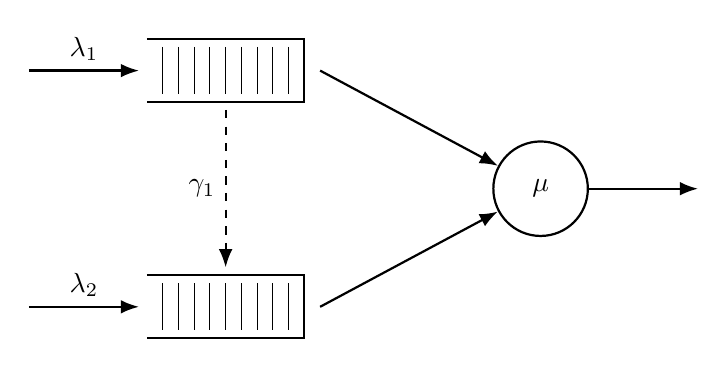
\begin{tikzpicture}[>=Latex, thick]

    % ── Queue 1 (top, Class-1, priority) ──────────────────────────────────────
    \draw (0, 1.9) -- (2, 1.9) -- (2, 1.1) -- (0, 1.1);
    \foreach \x in {0.2, 0.4, ..., 1.8} { \draw[thin] (\x, 1.8) -- (\x, 1.2); }
    \draw[->] (-1.5, 1.5) -- (-0.1, 1.5) node[midway, above] {$\lambda_1$};

    % ── Queue 2 (bottom, Class-2) ──────────────────────────────────────────────
    \draw (0, -1.1) -- (2, -1.1) -- (2, -1.9) -- (0, -1.9);
    \foreach \x in {0.2, 0.4, ..., 1.8} { \draw[thin] (\x, -1.2) -- (\x, -1.8); }
    \draw[->] (-1.5, -1.5) -- (-0.1, -1.5) node[midway, above] {$\lambda_2$};

    % ── One-way jockeying (1→2 only) ─────────────────────────────────────────
    \draw[->, dashed] (1.0, 1.0) -- (1.0, -1.0) node[midway, left] {$\gamma_1$};
    % No upward γ₂ arrow

    % ── Server ────────────────────────────────────────────────────────────────
    \node[draw, circle, minimum size=1.2cm] (server) at (5, 0) {$\mu$};
    \draw[->] (2.2,  1.5) -- (server);
    \draw[->] (2.2, -1.5) -- (server);
    \draw[->] (server) -- (7, 0);

\end{tikzpicture}
%
    }
    \caption{Queue layout for Model-$B_2$. Only the $1\to2$ jockeying direction
    is active (dashed, downward): class-1 customers may defect to Queue~2,
    but no customer can move in the reverse direction ($\gamma_2=0$).}
    \label{fig:model-b2-queue}
\end{figure}

\subsection{Reduced fundamental equation}\label{ssec:B2:reduction}

Setting $\gamma_2=0$ and $\theta_1=\theta_2=0$ in the general fundamental equation~\eqref{eq:gen:fundamental_equation} (Lemma~\ref{lem:gen:fundamental_equation}) annihilates the derivative terms in $y$, leaving:
\begin{align}
    &\bigl[(\lambda_1+\lambda_2+\mu)xy - \mu y - \lambda_1 x^2 y - \lambda_2 xy^2\bigr]P
    + \gamma_1 xy(x-y)\,\frac{\partial P}{\partial x} \nonumber \\
    &\qquad = \mu(x-y)\,P_y(y) - \mu x(1-y)\,\pi(0,0).
    \label{eq:B2:fundamental}
\end{align}
For each fixed $y\in(0,1]$ this is a first-order linear ODE in $x$; the entire analysis
of this section is built on it.

\begin{theorem}\label{thm:B2:PGF}
    Consider the two-class non-preemptive priority queueing system of Model-$B_2$ with
    per-customer jockeying rate $\gamma_1>0$ from Queue~1 to Queue~2 ($\gamma_2=0$,
    $\theta_1=\theta_2=0$). Under the stability condition $\rho=\lambda/\mu<1$,
    $\lambda=\lambda_1+\lambda_2$, the boundary generating function is
    \begin{equation}
        P_y(y) = \frac{\mu\,\pi(0,0)}{\mu-\lambda y}
        \cdot\frac{{}_1F_1\!\bigl(\alpha(y)+1;\,b^\star(y);\,-\lambda_1 y/\gamma_1\bigr)}
                  {{}_1F_1\!\bigl(\alpha(y);\,b^\star(y);\,-\lambda_1 y/\gamma_1\bigr)},
        \label{eq:B2:Py_thm}
    \end{equation}
    and the bivariate PGF, for $0\le x\le y$, is
    \begin{align}
        P(x,y) &= \frac{\mu\,e^{\lambda_1 x/\gamma_1}\,x^{-\alpha}(y-x)^{-\beta}}{\gamma_1 y}
        \Bigl[P_y(y)\,\mathcal{H}_1(x,y)
              + (1-y)\pi(0,0)\,\mathcal{H}_2(x,y)\Bigr],
        \label{eq:B2:Pxy}
    \end{align}
    where ${}_1F_1$ is Kummer's confluent hypergeometric function, the exponents are
    \begin{equation}
        \alpha(y) = \frac{\mu}{\gamma_1 y}, \qquad
        \beta(y)  = \frac{(1-y)(\lambda y-\mu)}{\gamma_1 y}, \qquad
        b^\star(y) = \alpha+\beta+1 = \frac{\mu+\lambda(1-y)+\gamma_1}{\gamma_1},
        \label{eq:B2:exponents_thm}
    \end{equation}
    the auxiliary integrals are
    \begin{align}
        \mathcal{H}_1(x,y) &= \int_0^x e^{-\lambda_1 t/\gamma_1}\,t^{\,\alpha-1}(y-t)^{\beta}\,dt,
        \label{eq:B2:I1}\\
        \mathcal{H}_2(x,y) &= \int_0^x e^{-\lambda_1 t/\gamma_1}\,t^{\,\alpha}(y-t)^{\beta-1}\,dt,
        \label{eq:B2:I2}
    \end{align}
    and the empty-state probability $\pi(0,0)=\rho(1-\rho)$ is given by Corollary~\ref{cor:B2:pi00} below.
    On $y<x\le1$ the same expression~\eqref{eq:B2:Pxy} holds with $\mathcal{H}_1,\mathcal{H}_2$
    replaced by their finite-part continuations; that the right-hand side is genuinely analytic
    across the interior point $x=y$ is the content of the smoothness condition established in
    Step~(ii) of the proof.
\end{theorem}

In the same fashion as in for Model-$B$, the result below is stated as a corollary in order for it to stay at the same level of hierarchy as that of other models.
\begin{corollary}\label{cor:B2:pi00}
    The empty-system probability $\pi_0$ (server idle, no one waiting) and the
    both-queues-empty probability $\pi(0,0)$ (server busy, $N_1=N_2=0$) of Model-$B_2$ are
    \begin{equation*}
        \pi_0 = 1-\rho, \qquad \pi(0,0) = \rho(1-\rho),
    \end{equation*}
    identical to the Model-$A$ baseline.
\end{corollary}
As in for Model-$B$, the proof follows trivially by setting $x=y=z$ in our fundamental equation (Equation~\eqref{eq:B2:fundamental}). The surviving equation is identical to the homologous in Model-$A$, and the result is proven in Corollary~\ref{cor:A:pi0}.

The proof of Theorem~\ref{thm:B2:PGF} consists of three steps: (i) obtaining the the standard form and the integration factor, (ii) determining $P_y(y)$ by analyticity in $x=y$, and (iii) recovering $P(x,y)$.

\begin{proof}[Proof of Theorem~\ref{thm:B2:PGF}]

% ─────────────────────────────────────────────────────────────────
\noindent\textit{Step~(i): Standard form and the integrating factor.}
\medskip

Fix $y\in(0,1]$, cancel a factor $y$ on both sides and divide the reduced fundamental equation~\eqref{eq:B2:fundamental} by the derivative term in $x$. The equation takes standard form $\tfrac{dP}{dx}+p(x;y)\,P=q(x;y)$ of \S\ref{sssec:if} (Equation~\eqref{eq:ode:standard}), with
\begin{align}
    \begin{split}
        p(x;y) &= \frac{(\lambda_1+\lambda_2+\mu)x - \mu - \lambda_1 x^2 - \lambda_2 xy}{\gamma_1 x(x-y)},
        \label{eq:B2:pxy}\\[4pt]
    \end{split} \\
    \begin{split}
        q(x;y) &= \frac{\mu\,P_y(y)}{\gamma_1 xy} - \frac{\mu(1-y)\,\pi(0,0)}{\gamma_1 y(x-y)}.
        \label{eq:B2:qxy}
    \end{split}
\end{align}
Write the numerator of $p$ as a polynomial in $x$,
\begin{equation*}
    N(x) = -\lambda_1 x^2 + \bigl[(\lambda_1+\lambda_2+\mu)-\lambda_2 y\bigr]x - \mu
         = -\lambda_1\bigl(x-x^*(y)\bigr)\bigl(x-x^+(y)\bigr),
\end{equation*}
where the roots $x^*(y),x^+(y)$ are those found for the kernel in Model-$A$ (Equation~\eqref{eq:A:xstar}), with , with $\lambda_1 x^* x^+ = \mu$ following from Vieta's formula. The Partial Fraction Decomposition of $p = N(x)/\bigl[\gamma_1 x(x-y)\bigr]$ read as rollows:
\begin{align*}
    A &= -\lambda_1, \nonumber\\
    B &= \frac{N(0)}{0-y} = \frac{-\mu}{-y} = \frac{\mu}{y}, \nonumber\\
    C &= \frac{N(y)}{y} = \frac{-(\lambda y-\mu)(y-1)}{y}
       = \frac{(1-y)(\lambda y-\mu)}{y},
\end{align*}
with $N(y)=-\lambda y^2+(\lambda+\mu)y-\mu=-(\lambda y-\mu)(y-1)$. Thus
\begin{equation}
    p(x;y) = \frac{1}{\gamma_1}\!\left[
        -\lambda_1 + \frac{\mu/y}{x} + \frac{(1-y)(\lambda y-\mu)/y}{x-y}
    \right].
    \label{eq:B2:pfrac}
\end{equation}

Since we will have a factor $(x-y)$ due to jockeying. we work on the region $0\leq x\leq y$, where $x-y\le0$; the complementary region $y<x\le1$ is recovered later. On this region, a term $\beta\ln|x-y|$ becomes simply $\beta\ln(y.-x)$, so integrating the partial fraction \eqref{eq:B2:pfrac} yields, up to a constant,
\begin{align*}
    \int^{x}\! p(t;y)\,dt
    &= \frac{1}{\gamma_1}\Bigl[-\lambda_1 x + \frac{\mu}{y}\ln x
       + \frac{(1-y)(\lambda y-\mu)}{y}\,\ln(y-x)\Bigr] \\
    &= -\frac{\lambda_1}{\gamma_1}\,x + \alpha(y)\ln x + \beta(y)\ln(y-x),
\end{align*}
with the exponents $\alpha(y)=\mu/(\gamma_1 y)>0$ and $\beta(y)=(1-y)(\lambda y-\mu)/(\gamma_1 y)$of~\eqref{eq:B2:exponents_thm}. Exponentiating, and dropping the multiplicative constant to which an integrating factor is indifferent, gives our integrating factor
\begin{equation*}
    \mu_I(x;y) = e^{-\lambda_1 x/\gamma_1}\,x^{\,\alpha(y)}\,(y-x)^{\,\beta(y)},
\end{equation*}
real-valued in our region because we take the base $(y-x)>0$ rather than $(x-y)$; its reciprocal $1/\mu_I$ is the homogeneous solution, playing here the role that $P_h$ played for Model-$B$ (\S\ref{sssec:vop}). It indeed solves $\mu_I'/\mu_I=p$:
\begin{align*}
    \frac{\mu_I'(x;y)}{\mu_I(x;y)}
    &= -\frac{\lambda_1}{\gamma_1} + \frac{\alpha}{x} + \beta\,\frac{d}{dx}\ln(y-x) \\
    &= -\frac{\lambda_1}{\gamma_1} + \frac{\alpha}{x} + \frac{\beta}{x-y}
     = p(x;y).
\end{align*}
The general solution of \S\ref{sssec:if} (Equation~\eqref{eq:ode:general}) now applies, and its arbitrary function is fixed immediately: since $\alpha>0$ we have $\mu_I\to0$ as $x\to0^{+}$, so the boundary contribution $P(0,y)\,\mu_I(0;y)$ vanishes and integrating $\tfrac{d}{dx}[P\,\mu_I]=q\,\mu_I$ over $(0,x]$ leaves
\begin{equation*}
    P(x,y)\,\mu_I(x;y) = \int_0^x q(t;y)\,\mu_I(t;y)\,dt.
\end{equation*}
Multiplying $q$ from~\eqref{eq:B2:qxy} by $\mu_I$ and applying the identity
$(y-t)^{\beta}/(t-y)=-(y-t)^{\beta-1}$ to the second term, the integrand separates into two pieces,
\begin{equation*}
    q(t;y)\,\mu_I(t;y) = \frac{\mu}{\gamma_1 y}\Bigl[
        P_y(y)\,e^{-\lambda_1 t/\gamma_1}\,t^{\,\alpha-1}(y-t)^{\beta}
        + (1-y)\pi(0,0)\,e^{-\lambda_1 t/\gamma_1}\,t^{\,\alpha}(y-t)^{\beta-1}
    \Bigr],
\end{equation*}
With the auxiliary integrals $\mathcal{H}_1,\mathcal{H}_2$ of~\eqref{eq:B2:I1}--\eqref{eq:B2:I2} and dividing through by $\mu_I(x;y)=e^{-\lambda_1 x/\gamma_1}x^{\alpha}(y-x)^{\beta}$, the solution on the principal region $0\le x\le y$ is
\begin{equation}
    P(x,y) = \frac{\mu\,e^{\lambda_1 x/\gamma_1}\,x^{-\alpha}(y-x)^{-\beta}}{\gamma_1 y}
    \Bigl[P_y(y)\,\mathcal{H}_1(x,y) + (1-y)\pi(0,0)\,\mathcal{H}_2(x,y)\Bigr],
    \label{eq:B2:Pxy_real}
\end{equation}
which still contains the unknown boundary function $P_y(y)$; Step~(ii) determines it.

% ─────────────────────────────────────────────────────────────────
\medskip\noindent\textit{Step~(ii): Determine $P_y(y)$ by analyticity at $x=y$.}
\medskip

Under stability —$\rho\leq1$— $\mu-\lambda y>0$ for $y\in(0,1)$, so the second exponent is negative:
\begin{equation}
    \beta(y) = \frac{(1-y)(\lambda y-\mu)}{\gamma_1 y} < 0,
    \qquad 0<y<1.
    \label{eq:B2:beta_negative}
\end{equation}
So the prefactor $(y-x)^{-\beta}=(y-x)^{|\beta|}$ in~\eqref{eq:B2:Pxy_real} \emph{vanishes} as $x\to y^{-}$, while $\mathcal{H}_1,\mathcal{H}_2$ may \emph{diverge}: the product is an indeterminate $0\cdot\infty$ form, whose resolution fixes $P_y(y)$.

On the diagonal the value is known outright. Setting $x=y$ in the fundamental
equation~\eqref{eq:B2:fundamental} drops the jockeying and boundary terms (each carries a
factor $x-y$) and leaves Model~$A$'s balance, so
\begin{equation}
    P(y,y) = \frac{\rho(1-\rho)}{1-\rho y},
    \label{eq:B2:regular_value}
\end{equation}
the diagonal value~\eqref{eq:A:Pzz}.

\smallskip\noindent\textit{Smoothness condition and $P_y(y)$.}
Pull the analytic, non-vanishing prefactor of~\eqref{eq:B2:Pxy_real} into
$\Psi(x)=\mu\,e^{\lambda_1 x/\gamma_1}x^{-\alpha}/(\gamma_1 y)$, so that
\begin{equation*}
    P(x,y)=\Psi(x)\,(y-x)^{|\beta|}
        \bigl[\,P_y(y)\,\mathcal{H}_1(x,y)+(1-y)\pi(0,0)\,\mathcal{H}_2(x,y)\,\bigr],
    \qquad |\beta|=-\beta>0 .
\end{equation*}
We need only the leading behaviour of the two integrals as $x\to y^{-}$, not a full expansion.
Each splits into its endpoint value $\mathcal{H}_i(y,y)=\int_0^y(\cdots)\,dt$ and a remainder
set by the integrand near $t=y$ --- $\mathcal{H}_1$ carries $(y-t)^{\beta}$, $\mathcal{H}_2$
carries $(y-t)^{\beta-1}$ --- so that, with constants $c_1,c_2$ whose values we never need,
\begin{equation*}
    \mathcal{H}_1(x,y)=\mathcal{H}_1(y,y)+c_1\,(y-x)^{\beta+1}+\cdots, \qquad
    \mathcal{H}_2(x,y)=\mathcal{H}_2(y,y)+c_2\,(y-x)^{\beta}+\cdots .
\end{equation*}
Multiplied by $(y-x)^{-\beta}$, the $c_1,c_2$ remainders turn into a smooth $O(y-x)$ term and the
constant regular value~\eqref{eq:B2:regular_value}; only the endpoint values retain the bare,
non-integer power $(y-x)^{|\beta|}$ ($|\beta|\notin\mathbb{Z}$ generically). Since $P(\cdot,y)$
is a power series in $x$ --- hence smooth at the interior point $x=y<1$, whereas that power is
not --- its coefficient must vanish:
\begin{equation}
    P_y(y)\,\mathcal{H}_1(y,y) + (1-y)\,\pi(0,0)\,\mathcal{H}_2(y,y) = 0 ,
    \label{eq:B2:nobranch}
\end{equation}
the endpoint integrals being read, since $\beta<0$, as the Euler--Beta continuations found next.
To evaluate these endpoint integrals, substitute $t=ys$ ($dt=y\,ds$)
in~\eqref{eq:B2:I1}--\eqref{eq:B2:I2}, which rescales the two integrands and pulls out a common
$y^{\alpha+\beta}$,
\begin{align*}
    t^{\alpha-1}(y-t)^{\beta}\,dt &= y^{\alpha+\beta}\,s^{\alpha-1}(1-s)^{\beta}\,ds, \\
    t^{\alpha}(y-t)^{\beta-1}\,dt &= y^{\alpha+\beta}\,s^{\alpha}(1-s)^{\beta-1}\,ds,
\end{align*}
so that, with $c:=\lambda_1 y/\gamma_1$,
\[
    \mathcal{H}_1(y,y)=y^{\alpha+\beta}\!\int_0^1\! s^{\alpha-1}(1-s)^{\beta}e^{-cs}\,ds,
    \qquad
    \mathcal{H}_2(y,y)=y^{\alpha+\beta}\!\int_0^1\! s^{\alpha}(1-s)^{\beta-1}e^{-cs}\,ds.
\]
These are Euler integrals~\eqref{eq:kummer:euler},
$\int_0^1 t^{a-1}(1-t)^{b-1}e^{zt}\,dt=B(a,b)\,{}_1F_1(a;a+b;z)$, with
$(a,b,z)=(\alpha,\beta+1,-c)$ for $\mathcal{H}_1$ and $(\alpha+1,\beta,-c)$ for
$\mathcal{H}_2$, so $a+b=b^\star(y)$ in both. As $\beta<0$ by~\eqref{eq:B2:beta_negative}, the
right-hand side is read as its analytic continuation in $b$ beyond the convergence range $b>0$,
giving
\begin{align}
    \mathcal{H}_1(y,y)
        &= B(\alpha,\,\beta+1)\,y^{\alpha+\beta}\,
           {}_1F_1\!\bigl(\alpha;\,b^\star(y);\,-\lambda_1 y/\gamma_1\bigr),
    \label{eq:B2:fp1}\\[3pt]
    \mathcal{H}_2(y,y)
        &= B(\alpha+1,\,\beta)\,y^{\alpha+\beta}\,
           {}_1F_1\!\bigl(\alpha+1;\,b^\star(y);\,-\lambda_1 y/\gamma_1\bigr).
    \label{eq:B2:fp2}
\end{align}
Solving the smoothness condition~\eqref{eq:B2:nobranch} for $P_y(y)$ and inserting the
endpoint values~\eqref{eq:B2:fp1}--\eqref{eq:B2:fp2}, the common factor $y^{\alpha+\beta}$
cancels and
\begin{equation}
    P_y(y)
    = -(1-y)\,\pi(0,0)\,\frac{\mathcal{H}_2(y,y)}{\mathcal{H}_1(y,y)}
    = -(1-y)\,\pi(0,0)\,\frac{B(\alpha+1,\,\beta)}{B(\alpha,\,\beta+1)}\,
        \frac{{}_1F_1\!\bigl(\alpha+1;\,b^\star;\,-\lambda_1 y/\gamma_1\bigr)}
             {{}_1F_1\!\bigl(\alpha;\,b^\star;\,-\lambda_1 y/\gamma_1\bigr)}.
    \label{eq:B2:Py_ratio}
\end{equation}
The Beta ratio reduces, via $\Gamma(\alpha+1)=\alpha\Gamma(\alpha)$ and
$\Gamma(\beta+1)=\beta\Gamma(\beta)$, to
\begin{align}
    \frac{B(\alpha+1,\,\beta)}{B(\alpha,\,\beta+1)}
    &= \frac{\Gamma(\alpha+1)\Gamma(\beta)}{\Gamma(\alpha+\beta+1)}
       \cdot\frac{\Gamma(\alpha+\beta+1)}{\Gamma(\alpha)\Gamma(\beta+1)} \nonumber\\
    &= \frac{\Gamma(\alpha+1)}{\Gamma(\alpha)}\cdot\frac{\Gamma(\beta)}{\Gamma(\beta+1)}
       = \frac{\alpha}{\beta},
    \label{eq:B2:beta_ratio}
\end{align}
and the surviving prefactor simplifies, using
$\alpha/\beta=\mu/\bigl[(1-y)(\lambda y-\mu)\bigr]$, as
\begin{align}
    -(1-y)\,\frac{\alpha}{\beta}
    &= -(1-y)\cdot\frac{\mu}{(1-y)(\lambda y-\mu)} \nonumber\\
    &= -\frac{\mu}{\lambda y-\mu} = \frac{\mu}{\mu-\lambda y}.
    \label{eq:B2:prefactor_combo}
\end{align}
Substituting~\eqref{eq:B2:beta_ratio}--\eqref{eq:B2:prefactor_combo}
into~\eqref{eq:B2:Py_ratio} gives the boundary generating function
\begin{align}
    P_y(y) &= \frac{\mu\,\pi(0,0)}{\mu-\lambda y}
    \cdot\frac{{}_1F_1\!\bigl(\alpha(y)+1;\,b^\star(y);\,-\lambda_1 y/\gamma_1\bigr)}
              {{}_1F_1\!\bigl(\alpha(y);\,b^\star(y);\,-\lambda_1 y/\gamma_1\bigr)},
    \label{eq:B2:Py}
\end{align}
confirming~\eqref{eq:B2:Py_thm}.  The prefactor equals the regular value $P(y,y)$
of~\eqref{eq:B2:regular_value}, and the Kummer ratio is the boundary correction.
As $y\to0^+$ the argument $-\lambda_1 y/\gamma_1\to0$, so the ratio tends to $1$ and
$P_y(0)=\pi(0,0)$, consistent with
$P_y(0)=\sum_{n_2}\pi(0,n_2)\cdot0^{n_2}=\pi(0,0)$.

% ─────────────────────────────────────────────────────────────────
\medskip\noindent\textit{Step~(iii): Recovery of $P(x,y)$.}
\medskip

Substituting~\eqref{eq:B2:Py} into the real-form expression~\eqref{eq:B2:Pxy_real}
gives, for $0\le x\le y$,
\begin{align*}
    P(x,y) &= \frac{\mu\,e^{\lambda_1 x/\gamma_1}\,x^{-\alpha}(y-x)^{-\beta}}{\gamma_1 y}
    \biggl[
        \frac{\mu\,\pi(0,0)}{\mu-\lambda y}
        \cdot\frac{{}_1F_1\!\bigl(\alpha+1;\,b^\star;\,-\tfrac{\lambda_1 y}{\gamma_1}\bigr)}
                  {{}_1F_1\!\bigl(\alpha;\,b^\star;\,-\tfrac{\lambda_1 y}{\gamma_1}\bigr)}
        \cdot\mathcal{H}_1(x,y)
    \nonumber\\[4pt]
    &\hspace{5.8cm}
        + (1-y)\pi(0,0)\cdot\mathcal{H}_2(x,y)
    \biggr],
\end{align*}
which is the statement of the theorem (Equation~\eqref{eq:B2:Pxy}).
The smoothness condition~\eqref{eq:B2:nobranch} guarantees that this extends
analytically across $x=y$, with diagonal value
$P(y,y)=\rho(1-\rho)/(1-\rho y)$ as computed in~\eqref{eq:B2:regular_value}.
On $y<x\le1$ the same formula holds with $\mathcal{H}_1,\mathcal{H}_2$ read as their
finite-part continuations; $\pi(0,0)=\rho(1-\rho)$ from Corollary~\ref{cor:B2:pi00} makes
the solution fully explicit.
The recovery of Model-$A$ in the limit $\gamma_1\to0^{+}$ is deferred to
Remark~\ref{rem:B2:singular_limit} below, as the limit is singular and merits
separate discussion.
\end{proof}

\begin{remark}[The singular limit $\gamma_1\to0^{+}$]\label{rem:B2:singular_limit}
The no-jockeying limit $\gamma_1\to0^{+}$ is a \emph{singular} perturbation: the coefficient
$\gamma_1 xy(x-y)$ of the highest derivative $\partial_x P$ vanishes, so one must check that the
convection term itself, not merely its coefficient, disappears. It does. Each $P$ is a
probability generating function, so $|P|\le1$ on the closed unit polydisc uniformly in
$\gamma_1$, and Cauchy's estimate then bounds $\partial_x P$ uniformly on every compact subset
of the open polydisc; hence $\gamma_1 xy(x-y)\,\partial_x P\to0$ there. The fundamental
equation~\eqref{eq:B2:fundamental} therefore degenerates to the algebraic Model-$A$
equation~\eqref{eq:A:fundamental}, and the uniformly bounded family $\{P\}_{\gamma_1}$, being
normal, converges (in full, by uniqueness of the analytic solution) to the Model-$A$
PGF~\eqref{eq:A:PGF}. In particular the boundary function reduces to the Model-$A$
value~\eqref{eq:A:Py},
\begin{equation}
    P_y(y)\;\xrightarrow[\ \gamma_1\to0^{+}\ ]{}\;
    \pi(0,0)\,\frac{x^*(y)\,(1-y)}{x^*(y)-y},
    \label{eq:B2:Py_limit}
\end{equation}
with $x^*(y)$ the Model-$A$ kernel root~\eqref{eq:A:xstar}; this needs no special-function
asymptotics.

The same limit can be read off the closed form~\eqref{eq:B2:Py}. Its prefactor
$\mu\,\pi(0,0)/(\mu-\lambda y)=\pi(0,0)/(1-\rho y)$ is $\gamma_1$-independent,
so~\eqref{eq:B2:Py_limit} is equivalent to the Kummer ratio tending to
\begin{equation}
    \frac{{}_1F_1\!\bigl(\alpha+1;\,b^\star;\,-\lambda_1 y/\gamma_1\bigr)}
         {{}_1F_1\!\bigl(\alpha;\,b^\star;\,-\lambda_1 y/\gamma_1\bigr)}
    \;\xrightarrow[\ \gamma_1\to0^{+}\ ]{}\;
    (1-\rho y)\,\frac{x^*(y)\,(1-y)}{x^*(y)-y}.
    \label{eq:B2:ratio_limit}
\end{equation}
The factor $(1-\rho y)$ shows the ratio does \emph{not} tend to the bare
$x^*(y)(1-y)/(x^*(y)-y)$; the discrepancy is exactly the prefactor. This matches the
first-parameter three-term recurrence for ${}_1F_1$~\cite[\S13.3]{dlmf}: as $\gamma_1\to0^{+}$
the parameters $\alpha$, $b^\star$ and $c=\lambda_1 y/\gamma_1$ all grow like $1/\gamma_1$, and
the recurrence reduces at leading order to a quadratic whose admissible root
is~\eqref{eq:B2:ratio_limit}.
\end{remark}

% ─────────────────────────────────────────────────────────────────
\subsection{Mean queue lengths and mean waiting times}

\subsubsection*{Total queue length from the diagonal}

Setting $x=y=z$ in the reduced fundamental equation~\eqref{eq:B2:fundamental}, the
jockeying convection term $\gamma_1 xy(x-y)\partial_xP$ vanishes at $x=y=z$
(factor $(x-y)=0$), as does the boundary term $\mu(x-y)P_y(y)$.  The remaining
balance is identical to Model-$A$'s, so the same diagonal cancellation gives
\[
    P(z,z) = \frac{\rho(1-\rho)}{1-\rho z},
\]
the same formula as~\eqref{eq:A:Pzz}.  Since $P(z,z)=\mathbb{E}[z^{N_1+N_2}]=\mathbb{E}[z^{N}]$
is the PGF of the total in-queue count $N$, the generating-function identity
$\tfrac{d}{dz}P(z,z)\big|_{z=1}=\mathbb{E}[N_1]+\mathbb{E}[N_2]$ holds;
differentiating by the quotient rule and evaluating at $z=1$:
\begin{align*}
    \mathbb{E}[N_1]+\mathbb{E}[N_2]
    &= \left.\frac{d}{dz}\,\frac{\rho(1-\rho)}{1-\rho z}\right|_{z=1}
     = \frac{\rho(1-\rho)\,\rho}{(1-\rho z)^2}\bigg|_{z=1} \\
    &= \frac{\rho^2(1-\rho)}{(1-\rho)^2}
     = \frac{\rho^2}{1-\rho}.
\end{align*}
One-way jockeying does not alter the total mean queue length relative to
Model-$A$, since the diagonal PGF is unchanged.

\subsubsection*{Class-1 mean queue length}

We extract $\mathbb{E}[N_1]=\tfrac{\partial P}{\partial x}\big|_{(1,1)}$ by first
reducing the fundamental equation~\eqref{eq:B2:fundamental} at $y=1$, and then
differentiating the resulting marginal PGF at $x=1$.

\medskip\noindent\textit{Step~1: marginal PGF $P(x,1)$.}\enspace
Evaluating~\eqref{eq:B2:fundamental} at $y=1$, the bracket multiplying $P$ becomes
$(\lambda_1+\mu)x-\mu-\lambda_1 x^2=-\lambda_1(x-1)(x-1/\rho_1)$, the convection
coefficient is $\gamma_1 x(x-1)$, and the right-hand side reduces to $\mu(x-1)P_y(1)$
(the $\pi(0,0)$ term carries the factor $(1-y)=0$). Every term therefore shares the common
factor $(x-1)$; cancelling it leaves the first-order linear ODE in $x$:
\[
    -\lambda_1(x-1/\rho_1)\,P(x,1) + \gamma_1 x\,\frac{d}{dx}P(x,1) = \mu\,P_y(1).
\]
The integrating factor for this ODE is $e^{-\lambda_1 x/\gamma_1}\,x^{\,\mu/\gamma_1}$
(noting $\lambda_1/\rho_1=\mu$), and integrating from $0$ to $x$ (the boundary term
vanishes since $0^{\mu/\gamma_1}=0$):
\[
    P(x,1)\,e^{-\lambda_1 x/\gamma_1}\,x^{\,\mu/\gamma_1}
    = \frac{\mu\,P_y(1)}{\gamma_1}
    \int_0^x e^{-\lambda_1 t/\gamma_1}\,t^{\,\mu/\gamma_1-1}\,dt.
\]
Rearranging and writing $\alpha=\mu/\gamma_1$ and
$\mathcal{H}(x)=\int_0^x e^{-\lambda_1 t/\gamma_1}\,t^{\,\alpha-1}\,dt$:
\[
    P(x,1) = \frac{\mu\,P_y(1)}{\gamma_1}\,e^{\lambda_1 x/\gamma_1}\,x^{-\alpha}\,\mathcal{H}(x).
\]
The constant $P_y(1)$ follows from $P(1,1)=1-\pi_0=\rho$, which gives
$P_y(1)=\rho\gamma_1/\bigl(\mu\,e^{\lambda_1/\gamma_1}\,\mathcal{H}(1)\bigr)$.

\medskip\noindent\textit{Step~2: differentiate $P(x,1)$ at $x=1$.}\enspace
Writing $P(x,1)=C\cdot f(x)\cdot\mathcal{H}(x)$ with $C=\mu P_y(1)/\gamma_1$ and
$f(x)=e^{\lambda_1 x/\gamma_1}\,x^{-\alpha}$, the product rule together with
Leibniz's rule ($d\mathcal{H}/dx = e^{-\lambda_1 x/\gamma_1}\,x^{\alpha-1}$, the integrand
at the upper limit) gives
\[
    \frac{d}{dx}P(x,1)
    = C\Bigl[f'(x)\,\mathcal{H}(x)+f(x)\,e^{-\lambda_1 x/\gamma_1}\,x^{\alpha-1}\Bigr].
\]
The logarithmic derivative $f'(x)/f(x)=\lambda_1/\gamma_1-\alpha/x=(\lambda_1 x-\mu)/(\gamma_1 x)$,
and the second product term simplifies as
$f(x)\,e^{-\lambda_1 x/\gamma_1}x^{\alpha-1}=x^{-1}$, so
\[
    \frac{d}{dx}P(x,1)
    = \frac{\mu\,P_y(1)}{\gamma_1}\left[
        e^{\lambda_1 x/\gamma_1}\,x^{-\alpha}\,\frac{\lambda_1 x-\mu}{\gamma_1 x}\,\mathcal{H}(x)
        + x^{-1}
    \right].
\]

\medskip\noindent\textit{Step~3: evaluate at $x=1$.}\enspace
\begin{align}
    \mathbb{E}[N_1]
    &= \left.\frac{d}{dx}P(x,1)\right|_{x=1} \nonumber\\
    &= \frac{\mu\,P_y(1)}{\gamma_1}\left[
        e^{\lambda_1/\gamma_1}\,\frac{\lambda_1-\mu}{\gamma_1}\,\mathcal{H}(1) + 1
    \right],
    \label{eq:B2:EN1}
\end{align}
where $\mathcal{H}(1)=\int_0^1 e^{-\lambda_1 t/\gamma_1}\,t^{\,\mu/\gamma_1-1}\,dt
=(\gamma_1/\lambda_1)^{\mu/\gamma_1}\,\gamma(\mu/\gamma_1,\,\lambda_1/\gamma_1)$
and $\gamma(\cdot,\cdot)$ is the lower incomplete gamma function.  The
factor $(\lambda_1-\mu)<0$ (since $\rho_1=\lambda_1/\mu<1$), confirming that
$e^{\lambda_1/\gamma_1}(\lambda_1-\mu)\mathcal{H}(1)/\gamma_1 + 1 > 0$.
No elementary simplification of~\eqref{eq:B2:EN1} is known; the expression
is evaluated numerically.  As $\gamma_1\to0^+$ the
Model-$A$ value~\eqref{eq:A:EN1} is recovered.

\subsubsection*{Class-2 mean queue length by subtraction}

\[
    \mathbb{E}[N_2]
    = \bigl(\mathbb{E}[N_1]+\mathbb{E}[N_2]\bigr)-\mathbb{E}[N_1]
    = \frac{\rho^2}{1-\rho}-\mathbb{E}[N_1].
\]
Since jockeying defections reduce the class-1 queue,
$\mathbb{E}[N_1]$ is smaller than the Model-$A$ value $\rho\rho_1/(1-\rho_1)$,
so $\mathbb{E}[N_2]$ correspondingly exceeds the Model-$A$ value.

\subsubsection*{Mean waiting times via Little's Law}

\textbf{Little's Law} applies here without qualification. It is a rate-conservation
identity --- for any subsystem in which customers are neither created nor destroyed
internally, the time-average number present equals the long-run entry rate times the mean
time an entrant spends inside --- and it holds for \emph{any} positive-recurrent system with
finite mean queue length (here ensured by $\rho<1$, which gives
$\mathbb{E}[N_1]\le\mathbb{E}[N]=\rho^2/(1-\rho)<\infty$ and so makes the jockeying rate
$\gamma_1\mathbb{E}[N_1]$ below a genuine finite rate), requiring neither Poisson input nor
independence. In particular it remains valid even
though one-way jockeying has destroyed the per-class Poisson/renewal structure (the very
obstruction that ruled out a probabilistic route in Step~(ii)). We apply it to each queue
(the waiting line, excluding the customer in service), with $\mathbb{E}[W_i]$ understood as
the mean time a customer spends in Queue~$i$ averaged over all customers that enter it ---
an arrival routed directly into service contributing a zero-length visit.

\emph{Class~1.} Every class-1 arrival is counted as an entrant to Queue~1 at rate
$\lambda_1$ (those finding the server idle enter service at once, contributing zero waiting
time), and each leaves Queue~1 either by entering service or by jockeying to Queue~2. Since
no other stream feeds Queue~1, its throughput is exactly $\lambda_1$, and Little's Law gives
\begin{equation}
    \mathbb{E}[W_1] = \frac{\mathbb{E}[N_1]}{\lambda_1}.
    \label{eq:B2:EW}
\end{equation}

\emph{Class~2.} Queue~2 has \emph{two} input streams: the class-2 Poisson arrivals at rate
$\lambda_2$ and the jockeying transfers from Queue~1. Because each of the $N_1$ waiting
class-1 customers jockeys independently at rate $\gamma_1$, the long-run transfer rate is
$\gamma_1\,\mathbb{E}[N_1]$ (a genuine rate by the ergodic theorem, equal to the time
average of the instantaneous jockeying intensity $\gamma_1 N_1$). The throughput of Queue~2
is therefore $\lambda_2+\gamma_1\,\mathbb{E}[N_1]$, and Little's Law reads
$\mathbb{E}[N_2]=\bigl(\lambda_2+\gamma_1\,\mathbb{E}[N_1]\bigr)\,\mathbb{E}[W_2]$, so that
\begin{equation}
    \mathbb{E}[W_2] = \frac{\mathbb{E}[N_2]}{\lambda_2+\gamma_1\,\mathbb{E}[N_1]}.
    \label{eq:B2:EW2}
\end{equation}
Here $\mathbb{E}[W_2]$ is the mean time in the class-2 line averaged over \emph{all} Queue-2
entrants of both streams; a jockeyed customer's Queue-2 clock starts at the transfer
instant, so its total wait is an initial Queue-1 segment (of mean $\mathbb{E}[W_1]$) followed
by this Queue-2 segment. Thus~\eqref{eq:B2:EW2} is the per-Queue-2-entrant residence time,
not the end-to-end delay of a tagged class-2 \emph{arrival}.

The jockeying inflow is what distinguishes~\eqref{eq:B2:EW2} from the single-stream
Models~$A$ and~$C_2$: the naive denominator $\lambda_2$ would undercount the entrants to
Queue~2 and is correct only in the no-jockeying limit. Indeed, as $\gamma_1\to0^{+}$ the
transfer rate $\gamma_1\,\mathbb{E}[N_1]\to0$, so~\eqref{eq:B2:EW2} reduces to
$\mathbb{E}[N_2]/\lambda_2$ and both~\eqref{eq:B2:EW} and~\eqref{eq:B2:EW2} recover the
Model-$A$ values~\eqref{eq:A:EW1}--\eqref{eq:A:EW2}.

\section{Analysis of Model-\texorpdfstring{$C_2$}{C2} (\texorpdfstring{$\theta_1>0,\,\gamma_1=\gamma_2=\theta_2=0$}{theta1>0, gamma1=gamma2=theta2=0})}\label{sec:model_c2}

In this section we derive $P(x,y)$ for the model in which only class-$1$ customers abandonment, but no class-$2$ abandonment and no jockeying. Figure~\ref{fig:model-c2-queue} shows the queue layout.
\begin{figure}[H]
    \centering
    \resizebox{0.62\textwidth}{!}{%
        % Model C₂: γ₁=γ₂=θ₂=0, θ₁>0
% Class-1 customers abandon the queue at rate θ₁ (dotted, upward from Queue 1).
% No jockeying. Class-2 never abandons.
\begin{tikzpicture}[>=Latex, thick]

    % ── Queue 1 (top, Class-1, priority) ──────────────────────────────────────
    \draw (0, 1.9) -- (2, 1.9) -- (2, 1.1) -- (0, 1.1);
    \foreach \x in {0.2, 0.4, ..., 1.8} { \draw[thin] (\x, 1.8) -- (\x, 1.2); }
    \draw[->] (-1.5, 1.5) -- (-0.1, 1.5) node[midway, above] {$\lambda_1$};
    % θ₁: Class-1 abandonment (dotted, upward)
    \draw[->, dotted] (1, 2.0) -- (1, 3.0) node[above] {$\theta_1$};

    % ── Queue 2 (bottom, Class-2) ──────────────────────────────────────────────
    \draw (0, -1.1) -- (2, -1.1) -- (2, -1.9) -- (0, -1.9);
    \foreach \x in {0.2, 0.4, ..., 1.8} { \draw[thin] (\x, -1.2) -- (\x, -1.8); }
    \draw[->] (-1.5, -1.5) -- (-0.1, -1.5) node[midway, above] {$\lambda_2$};
    % No θ₂: Class-2 does not abandon

    % ── Server ────────────────────────────────────────────────────────────────
    \node[draw, circle, minimum size=1.2cm] (server) at (5, 0) {$\mu$};
    \draw[->] (2.2,  1.5) -- (server);
    \draw[->] (2.2, -1.5) -- (server);
    \draw[->] (server) -- (7, 0);

\end{tikzpicture}
%
    }
    \caption{Queue layout for Model-$C_2$. Class-1 customers abandon the system
    at rate $\theta_1$ per waiting customer (dotted arrow, upward from Queue~1).
    Class-2 never abandons ($\theta_2=0$). There is no jockeying.}
    \label{fig:model-c2-queue}
\end{figure}
This choice of parameters is motivated by two key aspects of the resulting model: first, class-$2$ still sees Poisson arrivals, so the probabilistic argument of Model-$A$ carries over; second, substituting these values into the general fundamental equation~\eqref{eq:gen:fundamental_equation} leaves a first-order linear ODE in $x$, with no $y$-derivatives the boundary function $P_y(y)$ comes out of the integral, sparing us the Volterra equation that left Model-$B$ open (\S\ref{sec:model_b}).

\textbf{Stability.} Unlike the models without abandonment, stability here is non-trivial. The class-$1$ queue is an $M/M/1{+}M$ (Erlang-A) subsystem, which is positive recurrent for \emph{every} load (\S\ref{ssec:erlangA}); The only constraint comes from class-$2$, which —explained in more detail in \S\ref{ssec:C2:prob}— sees an $M/G/1$ queue whose service time is one class-$1$ busy period $B_C$. That queue is stable exactly when its utilisation stays below one:
\begin{equation}
    \lambda_2\,\mathbb{E}[B_C] \;<\; 1
    \qquad\Longleftrightarrow\qquad
    \rho_2\cdot{}_1F_1\!\left(1;\,\tfrac{\mu}{\theta_1}+1;\,\tfrac{\lambda_1}{\theta_1}\right) \;<\; 1,
    \label{eq:C2:stability}
\end{equation}
which follows from the mean busy period $\mathbb{E}[B_C]$ (Equation~\eqref{eq:erlangA:bp_mean}) together with the Kummer identity $\mu\bigl({}_1F_1(1;\tfrac{\mu}{\theta_1};\tfrac{\lambda_1}{\theta_1})-1\bigr)=\lambda_1\,{}_1F_1(1;\tfrac{\mu}{\theta_1}+1;\tfrac{\lambda_1}{\theta_1})$. Under the stability condition (Equation~\eqref{eq:C2:stability}), the PGF exists.

The following theorem states the result, obtained by both an analytical and a probabilistic methods:
\begin{theorem}\label{thm:C2:PGF}
    Consider the two-class non-preemptive priority system of Model-$C_2$ ($\theta_1>0$, $\gamma_1=\gamma_2=\theta_2=0$): Poisson arrivals at rates $\lambda_1,\lambda_2$, common exponential service at rate $\mu$, and per-customer abandonment of \emph{waiting} class-$1$ customers at rate $\theta_1$. Under the stability condition~\eqref{eq:C2:stability}, the probability generating function is
    \begin{align*}
        \begin{split}
            P(x,y) \;&=\; \frac{e^{\lambda_1 x/\theta_1}\,\mu\,\pi(0,0)\,(1-y)}{\theta_1\, x^{\mu/\theta_1}(1-x)^{\lambda_2(1-y)/\theta_1}\bigl(\widetilde{B}_C(\lambda_2(1-y))-y\bigr)}\\[4pt]
            &\quad\times \Bigl[\widetilde{B}_C(\lambda_2(1-y))\,\mathcal{H}_1(x,y) - \bigl(1-\widetilde{B}_C(\lambda_2(1-y))\bigr)\,\mathcal{H}_2(x,y)\Bigr],
        \end{split}
    \end{align*}
    where
    \begin{align*}
        \mathcal{H}_1(x,y) &\;=\; \int_0^x e^{-\lambda_1 t/\theta_1}\,t^{\,\mu/\theta_1-1}(1-t)^{\,\lambda_2(1-y)/\theta_1}\,dt, \\
        \mathcal{H}_2(x,y) &\;=\; \int_0^x e^{-\lambda_1 t/\theta_1}\,t^{\,\mu/\theta_1}(1-t)^{\,\lambda_2(1-y)/\theta_1-1}\,dt,
    \end{align*}
    $\widetilde{B}_C(s)$ is the LST of the busy period of the class-$1$ $M/M/1{+}M$ subsystem given by~\eqref{eq:erlangA:bp_lst}, and $\pi(0,0)$ is given by Corollary~\ref{cor:C2:pi00} below.
\end{theorem}

\begin{proof}
The proof consists of three steps:

\emph{Step~(i): reduction to a first-order ODE in $x$.}  Substituting the Model-$C_2$ parameters into the general fundamental equation (Equation~\eqref{eq:gen:fundamental_equation}) leaves, for each fixed $y$, a first-order linear ODE in $x$~\eqref{eq:C2:fundamental}. 
\begin{align}
    \begin{split}
            &\left[ (\lambda_1+\lambda_2+\mu)xy - \mu y - \lambda_1 x^2 y - \lambda_2 x y^2 \right] P(x,y)
        + \theta_1\, xy(x-1)\,\frac{\partial}{\partial x} P(x,y) \\
        & \quad=\quad \mu (x-y)\,P_y(y) - \mu x(1-y)\,\pi(0,0),
        \label{eq:C2:fundamental}
    \end{split} 
\end{align}
%TODO: Add brief Partial Fraction Decomposition, aligned with notation in Model-$B$

Its integrating factor (\S\ref{sssec:if}) is
\begin{equation*}
    \mu_I(x;y) \;=\; e^{-\lambda_1 x/\theta_1}\,x^{\alpha}\,(1-x)^{\beta(y)},
    \qquad \alpha=\tfrac{\mu}{\theta_1},\quad \beta(y)=\tfrac{\lambda_2(1-y)}{\theta_1},
\end{equation*}
which vanishes at $x=0$ and, for $y<1$, at $x=1$, since $\alpha>0$ and $\beta(y)\ge0$.

\emph{Step~(ii): determination of $P_y(y)$.}  We obtain $P_y(y)$ two independent ways.  \emph{Analytically} (\S\ref{ssec:C2:anal}), boundedness of $P(x,y)$ as $x\to1$ forces $\int_0^1 q(t;y)\,\mu_I(t;y)\,dt=0$~\eqref{eq:C2:boundedness}, which the Euler--Kummer identity~\eqref{eq:C2:Bc_Kummer} solves to give $P_y(y)$~\eqref{eq:C2:Py}.  \emph{Probabilistically} (\S\ref{ssec:C2:prob}), class-$2$ sees an $M/G/1$ queue with service time $B_C$, and the Pollaczek--Khinchine formula returns the same $P_y(y)$.

\emph{Step~(iii): recovery of $P(x,y)$.}  With $P_y(y)$ known, integrating the ODE against $\mu_I$ (\S\ref{ssec:C2:recovery}) yields the closed form~\eqref{eq:C2:Pxy}.
\end{proof}

\begin{corollary}\label{cor:C2:pi00}
    The limiting probability $\pi(0,0)$ of the busy state with both queues empty, and the empty-system probability $\pi_0$, are
    \begin{align}
        \pi(0,0) \;&=\; \frac{(\lambda_1+\lambda_2)\bigl(1 - \lambda_2\,\mathbb{E}[B_C]\bigr)}{\mu\,\bigl(1 + \lambda_1\,\mathbb{E}[B_C]\bigr)} \;=\; (\rho_1+\rho_2)\,\frac{1 - \lambda_2\,\mathbb{E}[B_C]}{1 + \lambda_1\,\mathbb{E}[B_C]}, \label{eq:C2:pi00}\\[4pt]
        \pi_0 \;&=\; \frac{1 - \lambda_2\,\mathbb{E}[B_C]}{1 + \lambda_1\,\mathbb{E}[B_C]}, \label{eq:C2:pi0}
    \end{align}
    where $\mathbb{E}[B_C]$ is the mean class-$1$ busy period~\eqref{eq:erlangA:bp_mean}. As $\theta_1\to 0^+$, $\mathbb{E}[B_C]\to (\mu-\lambda_1)^{-1}$ and these recover the Model-$A$ baseline $\pi(0,0) = \rho(1-\rho)$, $\pi_0 = 1-\rho$.
\end{corollary}

\subsection{Reduced fundamental equation}\label{ssec:C2:reduction}

Setting $\theta_1>0$ and $\gamma_1=\gamma_2=\theta_2=0$ in the general fundamental equation~\eqref{eq:gen:fundamental_equation} (Lemma~\ref{lem:gen:fundamental_equation}) annihilates the $\partial P/\partial y$ term outright---its coefficient $xy\bigl[\gamma_2(y-x)+\theta_2(y-1)\bigr]$ vanishes identically---and trims the $\partial P/\partial x$ coefficient $xy\bigl[\gamma_1(x-y)+\theta_1(x-1)\bigr]$ down to its surviving abandonment part $\theta_1\,xy(x-1)$. What remains is
\begin{multline}
    \left[ (\lambda_1+\lambda_2+\mu)xy - \mu y - \lambda_1 x^2 y - \lambda_2 x y^2 \right] P(x,y)
    + \theta_1\, xy(x-1)\,\frac{\partial}{\partial x} P(x,y) \\
    \;=\; \mu (x-y)\,P_y(y) - \mu x(1-y)\,\pi(0,0),
    \label{eq:C2:remove}
\end{multline}
where, as in Model-$A$, the boundary function $P_y(y)=P(0,y)=\sum_{n_2\ge0} \pi(0,n_2)\,y^{n_2}$ is the partial PGF over the states with the server busy and the priority queue empty ($N_1=0$).

For each fixed $y$, \eqref{eq:C2:fundamental} is a first-order linear ODE in $x$ with two unknowns: $P(x,y)$ on $[0,1]^2$ and its boundary trace $P_y(y)$. We first pin $P_y(y)$ down (\S\S\ref{ssec:C2:anal}--\ref{ssec:C2:prob}) and then recover $P(x,y)$ (\S\ref{ssec:C2:recovery}).

The probabilistic route needs one identity. By the \emph{law of total expectation}, splitting $P_y(y)=\mathbb{E}[\mathbf{1}\{\text{busy},N_1=0\}\,y^{N_2}]$ over the event $\{\text{busy},N_1=0\}$ factors it into the mass of that event and the conditional PGF of $N_2$ given it:
\begin{equation}
    P_y(y) \;=\; \mathbb{P}(\text{busy},\, N_1=0)\,\cdot\,\mathbb{E}\!\left[y^{N_2} \,\big|\, \text{busy},\, N_1=0\right].
    \label{eq:C2:Py_prob_decomp}
\end{equation}

\subsection{Analytical derivation of \texorpdfstring{$P_y(y)$}{Py(y)} via boundedness at \texorpdfstring{$x=1$}{x=1}}\label{ssec:C2:anal}

The surviving abandonment factor $(x-1)$ places the operative singularity on the boundary $x=1$---the boundedness-pinning regime anticipated in Remark~\ref{rem:gen:reading}. Dividing~\eqref{eq:C2:fundamental} by the coefficient $\theta_1 xy(x-1)$ of the derivative puts it in the standard form~\eqref{eq:ode:standard} of \S\ref{sssec:if},
\begin{align*}
    \frac{\partial P}{\partial x} \;+\; \underbrace{\frac{(\lambda_1+\lambda_2+\mu)x - \mu - \lambda_1 x^2 - \lambda_2 xy}{\theta_1\,x(x-1)}}_{p(x;\,y)}\,P
    \;=\; \underbrace{\frac{\mu(x-y)\,P_y(y) - \mu x(1-y)\,\pi(0,0)}{\theta_1\,xy(x-1)}}_{q(x;\,y)}.
\end{align*}
The numerator of $p(x;y)$ is the kernel polynomial $A(x,y)$ of Model-$B$~\eqref{eq:B:Adef}, common to every model, with roots $x^*(y),x^+(y)$~\eqref{eq:A:xstar} satisfying $x^*(y)\,x^+(y)=\mu/\lambda_1$. Its partial-fraction decomposition is
\begin{equation*}
    \frac{A(x,y)}{x(x-1)} \;=\; -\lambda_1 + \frac{B}{x} + \frac{C}{x-1},
\end{equation*}
with $-\lambda_1$ the ratio of leading ($x^2$) coefficients, $B=A(0,y)/(0-1)=(-\mu)/(-1)=\mu$ by the cover-up rule at $x=0$, and $C=A(1,y)=\lambda_2(1-y)$ by the cover-up rule at $x=1$ (since $A(1,y)=(\lambda_1+\lambda_2+\mu)-\mu-\lambda_1-\lambda_2 y=\lambda_2(1-y)$). Thus
\begin{equation}
    p(x;y) \;=\; \frac{1}{\theta_1}\!\left[-\lambda_1 + \frac{\mu}{x} + \frac{\lambda_2(1-y)}{x-1}\right].
    \label{eq:C2:pfd}
\end{equation}
Integrating term by term, $\int p\,dx = \theta_1^{-1}\bigl[-\lambda_1 x + \mu\ln x + \lambda_2(1-y)\ln(1-x)\bigr]$, which exponentiates to the integrating factor
\begin{equation}
    \mu_I(x;y) \;=\; e^{-\lambda_1 x/\theta_1}\, x^{\alpha}\, (1-x)^{\beta(y)},
    \label{eq:C2:integrating_factor}
\end{equation}
where, in parallel with Model-$B_2$, we set
\begin{equation}
    \alpha \;=\; \frac{\mu}{\theta_1}, \qquad \beta(y) \;=\; \frac{\lambda_2(1-y)}{\theta_1}.
    \label{eq:C2:exponents}
\end{equation}
Both exponents are non-negative ($\alpha>0$ always; $\beta(y)\ge0$ for $y\in[0,1]$), so $\mu_I$ vanishes at $x=0$ and at $x=1$. By the integrating-factor solution~\eqref{eq:ode:general} of \S\ref{sssec:if}---with the boundary term $P(0,y)\,\mu_I(0;y)$ killed by $\mu_I(0;y)=0$---we obtain
\begin{equation}
    P(x,y) \;=\; \frac{1}{\mu_I(x;y)} \int_0^x q(t;y)\,\mu_I(t;y)\,dt.
    \label{eq:C2:Pxy_implicit}
\end{equation}

We now pin $P_y(y)$ by the same boundedness argument used for Model-$A$, watching $P(x,y)$ as $x\to 1$ for fixed $y\in[0,1)$: there $\beta(y)>0$, so $\mu_I(x;y)\to0$. (At $y=1$ the exponent $\beta(1)=0$ and $\mu_I(\,\cdot\,;1)$ no longer vanishes at $x=1$; the value $P_y(1)$ is then recovered by continuity, $y\to1^-$.) Since the left-hand side $P(x,y)$ of~\eqref{eq:C2:Pxy_implicit} stays bounded while $1/\mu_I(x;y)\to\infty$, the integral must vanish in the limit:
\begin{equation}
    \int_0^1 q(t;y)\,\mu_I(t;y)\,dt \;=\; 0.
    \label{eq:C2:boundedness}
\end{equation}
Substituting the explicit $q$ and $\mu_I$, the integrand is
\begin{equation*}
    q(t;y)\,\mu_I(t;y)
    \;=\; \frac{\mu\bigl[(t-y)\,P_y(y) - t(1-y)\,\pi(0,0)\bigr]}{\theta_1\,y}
    \cdot \frac{e^{-\lambda_1 t/\theta_1}\,t^{\alpha}(1-t)^{\beta(y)}}{t\,(t-1)},
\end{equation*}
where $t^{\alpha}/t=t^{\alpha-1}$ and the elementary identity $(1-t)^{\beta(y)}/(t-1)=-(1-t)^{\beta(y)-1}$ flips the sign and lowers the exponent. The constant prefactor $-\mu/(\theta_1 y)$, nonzero for $y\in(0,1]$, divides out of~\eqref{eq:C2:boundedness}, leaving
\begin{equation*}
    \int_0^1 e^{-\lambda_1 t/\theta_1}\,t^{\,\alpha-1}(1-t)^{\,\beta(y)-1}\bigl[(t-y)\,P_y(y) - t(1-y)\,\pi(0,0)\bigr]\,dt \;=\; 0.
\end{equation*}
Introduce the auxiliary integrals
\begin{align*}
    \mathcal{J}_0(y) &\;=\; \int_0^1 e^{-\lambda_1 t/\theta_1}\,t^{\,\alpha-1}(1-t)^{\,\beta(y)-1}\,dt, \\
    \mathcal{J}_1(y) &\;=\; \int_0^1 e^{-\lambda_1 t/\theta_1}\,t^{\,\alpha}(1-t)^{\,\beta(y)-1}\,dt.
\end{align*}
Distributing the bracket over $t^{\alpha-1}$, the term $t\cdot t^{\alpha-1}=t^{\alpha}$ feeds $\mathcal{J}_1$ and $t^{\alpha-1}$ feeds $\mathcal{J}_0$, so the integral becomes
\begin{align*}
    0 \;&=\; P_y(y)\!\int_0^1\! e^{-\lambda_1 t/\theta_1}\bigl(t^{\alpha}-y\,t^{\alpha-1}\bigr)(1-t)^{\beta(y)-1}\,dt
    \;-\; (1-y)\,\pi(0,0)\!\int_0^1\! e^{-\lambda_1 t/\theta_1}\,t^{\alpha}(1-t)^{\beta(y)-1}\,dt \\
    \;&=\; P_y(y)\bigl[\mathcal{J}_1(y) - y\,\mathcal{J}_0(y)\bigr] \;-\; (1-y)\,\pi(0,0)\,\mathcal{J}_1(y),
\end{align*}
which gives
\begin{equation}
    P_y(y) \;=\; \pi(0,0)\,(1-y)\,\frac{\mathcal{J}_1(y)}{\mathcal{J}_1(y) - y\,\mathcal{J}_0(y)}.
    \label{eq:C2:Py_anal_raw}
\end{equation}

It remains to evaluate the ratio $\mathcal{J}_1/\mathcal{J}_0$. Setting $a=\alpha=\mu/\theta_1$, $b=s/\theta_1$, $c=\lambda_1/\theta_1$, the Euler representation~\eqref{eq:kummer:euler} writes each $\mathcal{J}_i$ as a Beta multiple of a $\,{}_1F_1$ value, and the closed-form summation~\eqref{eq:erlangA:cf_kummer} of \S\ref{ssec:erlangA} identifies their ratio with the busy-period LST:
\begin{equation}
    \widetilde{B}_C(s) \;=\; \frac{\displaystyle\int_{0}^{1} t^{a}(1-t)^{b-1}e^{-ct}\,dt}{\displaystyle\int_{0}^{1} t^{a-1}(1-t)^{b-1}e^{-ct}\,dt}
    \;=\; \frac{B(a+1,b)\,{}_1F_1(a+1;\,a+1+b;\,-c)}{B(a,b)\,{}_1F_1(a;\,a+b;\,-c)}.
    \label{eq:C2:Bc_Kummer}
\end{equation}
Taking $s=\lambda_2(1-y)$---so that $b=\beta(y)$ matches the exponent in~\eqref{eq:C2:exponents}---gives $\widetilde{B}_C(\lambda_2(1-y))=\mathcal{J}_1(y)/\mathcal{J}_0(y)$. Dividing the numerator and denominator of~\eqref{eq:C2:Py_anal_raw} by $\mathcal{J}_0(y)$ yields the boundary generating function
\begin{equation}
    P_y(y) \;=\; \pi(0,0)\,\frac{(1-y)\,\widetilde{B}_C(\lambda_2(1-y))}{\widetilde{B}_C(\lambda_2(1-y)) - y}.
    \label{eq:C2:Py}
\end{equation}
This route uses no probabilistic structure: it reaches~\eqref{eq:C2:Py} through the Beta-integral identity~\eqref{eq:C2:Bc_Kummer} alone---the analytic shadow of the $M/G/1$/busy-period decomposition that the next subsection makes explicit.

\subsection{Probabilistic re-derivation of \texorpdfstring{$P_y(y)$}{Py(y)}}\label{ssec:C2:prob}

We again take the point of view of a class-$2$ customer waiting while the server is busy. Unlike when jockeying, class-$1$ customers here truly leave the system, so the class-$2$ Poisson arrival stream is undisturbed. the class-$2$ \emph{effective service time} is therefore one full busy period $B_C$ of the class-$1$ subsystem —now an $M/M/1{+}M$ queue with rates $\lambda_1,\mu,\theta_1$, rather than the pure $M/M/1$ of Model-$A$. So class-$2$ sees an $M/G/1$ queue with Poisson input $\lambda_2$ and service distributed as $B_C$. Its LST $\widetilde{B}_C(s)$ and mean $\mathbb{E}[B_C]$ come from the first-step analysis of \S\ref{ssec:erlangA} (Equations~\eqref{eq:erlangA:bp_lst} and \eqref{eq:erlangA:bp_mean}).

This $M/G/1$ is stable if and only if its utilisation $\lambda_2\,\mathbb{E}[B_C] < 1$ (Equation~\eqref{eq:C2:stability}). The condition is also strictly weaker than the no-abandonment requirement $\rho=\rho_1+\rho_2<1$.

Applying the Pollaczek-Khinchine formula~\eqref{eq:pk:pgf} with the identifications $\lambda\mapsto\lambda_2$, $\widetilde{B}\mapsto\widetilde{B}_C$, $\rho_B=\lambda_2\,\mathbb{E}[B_C]$ gives the PGF of the stationary number of class-$2$ customers in that $M/G/1$:
\begin{equation*}
    L_2(y) \;=\; \frac{(1 - \lambda_2 \mathbb{E}[B_C])\,(1-y)\,\widetilde{B}_C(\lambda_2(1-y))}{\widetilde{B}_C(\lambda_2(1-y)) - y}.
\end{equation*}
Since class-$2$ arrivals are Poisson-distributed, by \emph{PASTA} (\S\ref{ssec:priority}), the stationary number of class-$2$ customers is that of the $M/G/1$ at all times. Conditioning on $\{\text{busy},\,N_1=0\}$, we can identify that with that count with $N_2$:
\begin{equation}
    \mathbb{E}\!\left[y^{N_2} \,\big|\, \text{busy},\, N_1=0\right] \;=\; L_2(y).
    \label{eq:C2:L2_identification}
\end{equation}
Substituting~\eqref{eq:C2:L2_identification} into the decomposition~\eqref{eq:C2:Py_prob_decomp} gives
\begin{equation}
    P_y(y) \;=\; \mathbb{P}(\text{busy},\,N_1=0)\,\frac{(1-\lambda_2\mathbb{E}[B_C])\,(1-y)\,\widetilde{B}_C(\lambda_2(1-y))}{\widetilde{B}_C(\lambda_2(1-y)) - y}.
    \label{eq:C2:Py_unsimplified}
\end{equation}
The unknown mass $\mathbb{P}(\text{busy},N_1=0)$ is fixed by $P_y(0)=\pi(0,0)$: evaluating~\eqref{eq:C2:Py_unsimplified} at $y=0$, where $\widetilde{B}_C(\lambda_2)$ cancels,
\begin{align*}
    \pi(0,0)=P_y(0)
    &= \mathbb{P}(\text{busy},\,N_1=0)\,\frac{(1-\lambda_2\mathbb{E}[B_C])\cdot 1\cdot \widetilde{B}_C(\lambda_2)}{\widetilde{B}_C(\lambda_2)}
    &= \mathbb{P}(\text{busy},\,N_1=0)\,(1-\lambda_2\mathbb{E}[B_C]),
\end{align*}
so $\mathbb{P}(\text{busy},N_1=0)=\pi(0,0)/(1-\lambda_2\mathbb{E}[B_C])$. Substituting back, the factor $(1-\lambda_2\mathbb{E}[B_C])$ cancels and we recover
\begin{equation*}
    P_y(y) \;=\; \pi(0,0)\,\frac{(1-y)\,\widetilde{B}_C(\lambda_2(1-y))}{\widetilde{B}_C(\lambda_2(1-y)) - y},
\end{equation*}
which matches the result of Equation~\eqref{eq:C2:Py}, and so does match the expression as in the probabilistic argument for Model-$A$ (Equation~\eqref{eq:A:Py}); the only difference is the effective service time, now the busy period of an $M/M/1{+}M$ (Erlang-A) subsystem rather than of an ordinary $M/M/1$.

\subsection{Recovery of \texorpdfstring{$P(x,y)$}{P(x,y)} from \texorpdfstring{$P_y(y)$}{Py(y)}}\label{ssec:C2:recovery}

With $P_y(y)$ in hand, we return to the ODE~\eqref{eq:C2:fundamental} and substitute~\eqref{eq:C2:Py} into its right-hand side. Writing $\zeta(y)\equiv\widetilde{B}_C(\lambda_2(1-y))$ for brevity,
\begin{align*}
    \text{RHS}
    &\;=\; \mu(x-y)\,\pi(0,0)\,\frac{(1-y)\,\zeta(y)}{\zeta(y) - y} \;-\; \mu x(1-y)\,\pi(0,0) \\
    &\;=\; \mu\,\pi(0,0)\,(1-y)\!\left[\frac{(x-y)\,\zeta(y)}{\zeta(y) - y} - x\right] \\
    &\;=\; \mu\,\pi(0,0)\,(1-y)\,\frac{(x-y)\,\zeta(y) - x\bigl[\zeta(y) - y\bigr]}{\zeta(y) - y} \\
    &\;=\; \mu\,\pi(0,0)\,y(1-y)\,\frac{x - \zeta(y)}{\zeta(y) - y},
\end{align*}
which has the same form as the RHS of Model-$A$, now with the more involved service time $B_C$. With $p(x;y)$ and $\mu_I(x;y)$ as in~\eqref{eq:C2:pfd} and~\eqref{eq:C2:integrating_factor}, the standard-form source becomes
\begin{equation*}
    q(x;y) \;=\; \frac{\mu\,\pi(0,0)\,(1-y)\,\bigl[x-\zeta(y)\bigr]}{\theta_1\,x(x-1)\,\bigl[\zeta(y)-y\bigr]},
\end{equation*}
and~\eqref{eq:C2:Pxy_implicit} reads $P(x,y)=\mu_I(x;y)^{-1}\int_0^x q(t;y)\,\mu_I(t;y)\,dt$. To carry out the integral, use the partial fraction
\begin{equation*}
    \frac{t-\zeta(y)}{t(t-1)}
    \;=\; \frac{\zeta(y)(t-1) + t\bigl(1-\zeta(y)\bigr)}{t(t-1)}
    \;=\; \frac{\zeta(y)}{t} + \frac{1-\zeta(y)}{t-1},
\end{equation*}
and define the auxiliary integrals
\begin{align*}
    \mathcal{H}_1(x,y) &\;=\; \int_0^x e^{-\lambda_1 t/\theta_1}\,t^{\,\alpha-1}(1-t)^{\,\beta(y)}\,dt,  \\
    \mathcal{H}_2(x,y) &\;=\; \int_0^x e^{-\lambda_1 t/\theta_1}\,t^{\,\alpha}(1-t)^{\,\beta(y)-1}\,dt,
\end{align*}
with $\alpha,\beta(y)$ as in~\eqref{eq:C2:exponents}. These are the partial (upper limit $x$) counterparts of the full integrals of \S\ref{ssec:C2:anal}: $\mathcal{H}_2(1,y)=\mathcal{J}_1(y)$ exactly, whereas $\mathcal{H}_1(1,y)\neq\mathcal{J}_0(y)$ (its $(1-t)$ exponent is $\beta(y)$, not $\beta(y)-1$). The mismatch is harmless, as $\mathcal{H}_1$ and $\mathcal{H}_2$ only ever appear in the combination $\zeta\,\mathcal{H}_1-(1-\zeta)\,\mathcal{H}_2$.

Multiplying $q(t;y)$ by $\mu_I(t;y)=e^{-\lambda_1 t/\theta_1}t^{\alpha}(1-t)^{\beta(y)}$ and inserting the partial fraction, the integrand splits into the two pieces defining $\mathcal{H}_1,\mathcal{H}_2$:
\begin{align*}
    q(t;y)\,\mu_I(t;y)
    &\;=\; \frac{\mu\,\pi(0,0)\,(1-y)}{\theta_1\bigl(\zeta(y)-y\bigr)}
      \left[\frac{\zeta(y)}{t} + \frac{1-\zeta(y)}{t-1}\right]
      e^{-\lambda_1 t/\theta_1}\,t^{\alpha}(1-t)^{\beta(y)} \\
    &\;=\; \frac{\mu\,\pi(0,0)\,(1-y)}{\theta_1\bigl(\zeta(y)-y\bigr)}
      \Bigl[\zeta(y)\,e^{-\lambda_1 t/\theta_1}\,t^{\alpha-1}(1-t)^{\beta(y)}
      - \bigl(1-\zeta(y)\bigr)\,e^{-\lambda_1 t/\theta_1}\,t^{\alpha}(1-t)^{\beta(y)-1}\Bigr],
\end{align*}
the second term again using $(1-t)^{\beta(y)}/(t-1)=-(1-t)^{\beta(y)-1}$, which produces both the minus sign and the exponent shift on $\mathcal{H}_2$. Since $\pi(0,0)$ and $\zeta(y)$ leave the integral,
\begin{equation*}
    \int_0^x q(t;y)\,\mu_I(t;y)\,dt \;=\; \frac{\mu\,\pi(0,0)\,(1-y)}{\theta_1\bigl(\zeta(y)-y\bigr)}\Bigl[\zeta(y)\,\mathcal{H}_1(x,y) \;-\; \bigl(1-\zeta(y)\bigr)\,\mathcal{H}_2(x,y)\Bigr].
\end{equation*}
Dividing by $\mu_I(x;y)$ and restoring $\zeta(y)=\widetilde{B}_C(\lambda_2(1-y))$, we arrive at the closed form
\begin{align}
    \begin{split}
        P(x,y) \;=\; \frac{e^{\lambda_1 x/\theta_1}\,\mu\,\pi(0,0)\,(1-y)}{\theta_1\, x^{\alpha}(1-x)^{\beta(y)}\bigl(\widetilde{B}_C(\lambda_2(1-y))-y\bigr)}\\[4pt]
        \times \Bigl[\widetilde{B}_C(\lambda_2(1-y))\,\mathcal{H}_1(x,y) - \bigl(1-\widetilde{B}_C(\lambda_2(1-y))\bigr)\,\mathcal{H}_2(x,y)\Bigr],
    \end{split}\label{eq:C2:Pxy}
\end{align}
which is the statement of the theorem: the boundary function $P_y(y)$---obtained analytically in \S\ref{ssec:C2:anal} and probabilistically in \S\ref{ssec:C2:prob}---combined with the analytic integration of the ODE in $x$.

\begin{proof}[Proof of Corollary~\ref{cor:C2:pi00}]
    The fully idle state---server empty, no customer present, probability $\pi_0$---communicates with the rest of the chain through a single neighbour: the busy-and-empty state $(N_1,N_2)=(0,0)$ of probability $\pi(0,0)$, with exactly one customer in service and both queues empty (recall the standing convention $\pi_0\neq\pi(0,0)$). The system leaves the idle state only on an arrival of either class, at combined rate $\lambda_1+\lambda_2$ (Poisson superposition), and re-enters it only on the service completion that empties the busy-and-empty state, at rate $\mu$ (no abandonment can fire from $\pi(0,0)$, as both queues are empty). Global balance across the cut isolating the idle state (as in~\eqref{eq:gen:balance_idle}) therefore gives
    \begin{equation}
        (\lambda_1+\lambda_2)\,\pi_0 \;=\; \mu\,\pi(0,0),
        \label{eq:C2:balance_zero}
    \end{equation}
    so $\pi(0,0)=(\rho_1+\rho_2)\,\pi_0$.

    To fix $\pi_0$, we again use the $M/G/1$ structure of \S\ref{ssec:C2:prob}. By the $M/G/1$ utilisation identity, the long-run fraction of time this queue is busy is $\rho_B=\lambda_2\,\mathbb{E}[B_C]$, and ``idle'' means no class-$2$ customer is present, so
    \begin{equation*}
        \mathbb{P}(\text{no class-$2$ present}) \;=\; 1 - \lambda_2\,\mathbb{E}[B_C].
    \end{equation*}
    Conditional on no class-$2$ being present, the priority subsystem evolves as the $M/M/1{+}M$ queue ($\lambda_1,\mu,\theta_1$) defining $B_C$, alternating idle periods and busy periods $B_C$ in an \emph{alternating renewal process} whose regenerations are the instants it empties. An idle period lasts until the next class-$1$ arrival, which by memorylessness is $\mathrm{Exp}(\lambda_1)$ with mean $1/\lambda_1$, so the mean cycle is $1/\lambda_1+\mathbb{E}[B_C]$. By the \emph{renewal--reward theorem} the idle fraction is the ratio of mean idle period to mean cycle:
    \begin{equation*}
        \mathbb{P}(\text{class-$1$ absent} \mid \text{no class-$2$ present})
        \;=\; \frac{1/\lambda_1}{1/\lambda_1+\mathbb{E}[B_C]}
        \;=\; \frac{1}{1+\lambda_1\,\mathbb{E}[B_C]}.
    \end{equation*}
    The fully idle event is the intersection of $A=\{\text{class-$1$ absent}\}$ and $B=\{\text{no class-$2$ present}\}$, so by the chain rule $\mathbb{P}(A\cap B)=\mathbb{P}(B)\,\mathbb{P}(A\mid B)$ (not independence),
    \begin{equation*}
        \pi_0 \;=\; \bigl(1-\lambda_2\,\mathbb{E}[B_C]\bigr)\cdot\frac{1}{1+\lambda_1\,\mathbb{E}[B_C]} \;=\; \frac{1-\lambda_2\,\mathbb{E}[B_C]}{1+\lambda_1\,\mathbb{E}[B_C]},
    \end{equation*}
    which is~\eqref{eq:C2:pi0}; substituting into~\eqref{eq:C2:balance_zero} gives~\eqref{eq:C2:pi00}.

    In the limit $\theta_1\to 0^+$ the $M/M/1{+}M$ busy period collapses to the pure-$M/M/1$ one, $\mathbb{E}[B_C]\to(\mu-\lambda_1)^{-1}$, so
    \[
        \lambda_1\,\mathbb{E}[B_C]\to\frac{\rho_1}{1-\rho_1},
        \qquad
        \lambda_2\,\mathbb{E}[B_C]\to\frac{\rho_2}{1-\rho_1},
    \]
    whence $1+\lambda_1\,\mathbb{E}[B_C]\to1/(1-\rho_1)$ and $1-\lambda_2\,\mathbb{E}[B_C]\to(1-\rho)/(1-\rho_1)$. Therefore $\pi_0\to1-\rho$ by~\eqref{eq:C2:pi0}, and $\pi(0,0)=(\rho_1+\rho_2)\,\pi_0\to\rho(1-\rho)$, recovering the Model-$A$ baseline.
\end{proof}

\subsection{Mean queue lengths and mean waiting times}

\subsubsection*{Why the diagonal no longer simplifies}

Setting $x=y=z$ in~\eqref{eq:C2:fundamental}, the abandonment derivative term $\theta_1 xy(x-1)\,\partial_xP$ survives (the factor $(x-1)|_{x=z}\neq0$ for $z\in(0,1)$), and the diagonal equation reads
\begin{equation}
    \bigl[(\lambda_1{+}\lambda_2{+}\mu)z^2-\mu z-\lambda z^3\bigr]P(z,z)
    + \theta_1 z^2(z-1)\,\frac{\partial P}{\partial x}(z,z)
    \;=\; -\mu z(1-z)\,\pi(0,0).
    \label{eq:C2:diag}
\end{equation}
The contrast with Model-$A$ —or models without abandonment— is instructive: $P(z,z)$ is no longer purely algebraic with closed form $P(z,z)=\pi(0,0)/(1-\rho z)$~\eqref{eq:A:Pzz}, where the total number of customers $\mathbb{E}[N_1]+\mathbb{E}[N_2]$ followed easily by differentiation. Here the surviving derivative term remains as a second unknown so that path is no longer available since abandonment removes customers and lowers both means relative to models without abandonments.

\subsubsection*{Class-2 mean queue length via \texorpdfstring{$P(1,y)$}{P(1,y)}}

Setting $x=1$ in~\eqref{eq:C2:fundamental} we obtain
\begin{equation*}
    \lambda_2 y(1-y)\,P(1,y) \;=\; \mu(1-y)\bigl[P_y(y)-\pi(0,0)\bigr]. \\
\end{equation*}
Cancelling $(1-y)$ for $y\neq1$ and substituting the known $P_y(y)$~\eqref{eq:C2:Py},
\begin{equation*}
    P(1,y)
    \;=\; \frac{\mu\bigl[P_y(y)-\pi(0,0)\bigr]}{\lambda_2 y}
    \;=\; \frac{\mu\,\pi(0,0)}{\lambda_2}\cdot\frac{1-\widetilde{B}_C(\lambda_2(1-y))}{\widetilde{B}_C(\lambda_2(1-y))-y},
\end{equation*}
the marginal PGF of $N_2$. It is $0/0$ at $y=1$, so set $\varepsilon=1-y\to0$ and use the LST expansion $\widetilde{B}_C(\lambda_2\varepsilon)=1-\lambda_2\mathbb{E}[B_C]\,\varepsilon+\tfrac{1}{2}\lambda_2^2\mathbb{E}[B_C^2]\,\varepsilon^2+O(\varepsilon^3)$:
\begin{align*}
    1-\widetilde{B}_C(\lambda_2\varepsilon)
    &\;=\; \lambda_2\mathbb{E}[B_C]\,\varepsilon
           -\tfrac{1}{2}\lambda_2^2\mathbb{E}[B_C^2]\,\varepsilon^2+O(\varepsilon^3), \\
    \widetilde{B}_C(\lambda_2\varepsilon)-y
    &\;=\; \bigl(1-\lambda_2\mathbb{E}[B_C]\,\varepsilon+\tfrac{1}{2}\lambda_2^2\mathbb{E}[B_C^2]\,\varepsilon^2\bigr)-(1-\varepsilon)
    \;=\; (1-\lambda_2\mathbb{E}[B_C])\,\varepsilon
           +\tfrac{1}{2}\lambda_2^2\mathbb{E}[B_C^2]\,\varepsilon^2+O(\varepsilon^3).
\end{align*}
Writing $a=\lambda_2\mathbb{E}[B_C]$ and $c=\tfrac{1}{2}\lambda_2^2\mathbb{E}[B_C^2]$,
\begin{equation*}
    P(1,1-\varepsilon)
    \;=\; \frac{\mu\,\pi(0,0)}{\lambda_2}\cdot\frac{a\varepsilon - c\varepsilon^2+O(\varepsilon^3)}{(1-a)\varepsilon+c\varepsilon^2+O(\varepsilon^3)}
    \;=\; \frac{\mu\,\pi(0,0)}{\lambda_2}\cdot\frac{a-c\varepsilon}{(1-a)+c\varepsilon}+O(\varepsilon^2).
\end{equation*}
Differentiating $f(\varepsilon)=(a-c\varepsilon)/((1-a)+c\varepsilon)$ by the quotient rule,
\begin{equation*}
    f'(\varepsilon)
    \;=\; \frac{-c\,\bigl((1-a)+c\varepsilon\bigr)-(a-c\varepsilon)\,c}{\bigl((1-a)+c\varepsilon\bigr)^2}
    \;=\; \frac{-c}{(1-a+c\varepsilon)^2},
\end{equation*}
and since $\tfrac{d}{dy}P(1,y)\big|_{y=1}=-\tfrac{d}{d\varepsilon}P(1,1-\varepsilon)\big|_{\varepsilon=0}$,
\begin{equation}
    \mathbb{E}[N_2]
    \;=\; \frac{d}{dy}P(1,y)\bigg|_{y=1}
    \;=\; \frac{\mu\,\pi(0,0)}{\lambda_2}\cdot\frac{c}{(1-a)^2}
    \;=\; \frac{\mu\,\pi(0,0)\,\lambda_2\,\mathbb{E}[B_C^2]}{2\,(1-\lambda_2\mathbb{E}[B_C])^2}.
    \label{eq:C2:EN2}
\end{equation}
As $\theta_1\to0^+$, $\mathbb{E}[B_C]\to(\mu-\lambda_1)^{-1}$ and $\mathbb{E}[B_C^2]\to2\mu/(\mu-\lambda_1)^3$, recovering the Model-$A$ value $\mathbb{E}[N_2]=\rho\rho_2/((1-\rho_1)(1-\rho))$.

\subsubsection*{Class-1 mean queue length}

We extract $\mathbb{E}[N_1]=\tfrac{\partial P}{\partial x}\big|_{(1,1)}$ by evaluating the theorem formula at $y=1$ and then differentiating in $x$.

\medskip\noindent\textit{Step~1: marginal PGF $P(x,1)$.}\enspace
As $y\to1$, the exponent $\beta(y)\to0$, so $(1-x)^{\beta(y)}\to1$ for fixed $x\in(0,1)$, and $\mathcal{H}_1(x,y)\to\int_0^x e^{-\lambda_1 t/\theta_1}\,t^{\,\mu/\theta_1-1}\,dt$ while $\mathcal{H}_2(x,y)$ tends to a finite limit. In the theorem's bracket the two integrals carry different weights: $\widetilde{B}_C(\lambda_2(1-y))\to1$, while $1-\widetilde{B}_C(\lambda_2(1-y))=\lambda_2\mathbb{E}[B_C]\,(1-y)+O((1-y)^2)\to0$, so the $\mathcal{H}_2$ term drops and the bracket collapses to $\mathcal{H}_1(x,1)$. The prefactor's $y$-dependent part satisfies $(1-y)/(\widetilde{B}_C(\lambda_2(1-y))-y)\to1/(1-\lambda_2\mathbb{E}[B_C])$, so
\begin{equation*}
    P(x,1)
    \;=\; \frac{\mu\,\pi(0,0)}{\theta_1\,(1-\lambda_2\mathbb{E}[B_C])}\,e^{\lambda_1 x/\theta_1}\,x^{-\mu/\theta_1}
    \int_0^x e^{-\lambda_1 t/\theta_1}\,t^{\,\mu/\theta_1-1}\,dt.
\end{equation*}

\medskip\noindent\textit{Step~2: differentiate $P(x,1)$ at $x=1$.}\enspace
Write $P(x,1)=C\,f(x)\,\mathcal{K}(x)$ with $C=\mu\pi(0,0)/(\theta_1(1-\lambda_2\mathbb{E}[B_C]))$, $f(x)=e^{\lambda_1 x/\theta_1}x^{-\mu/\theta_1}$ and $\mathcal{K}(x)=\int_0^x e^{-\lambda_1 t/\theta_1}t^{\,\mu/\theta_1-1}\,dt$. By the product rule with Leibniz's rule ($\mathcal{K}'(x)=e^{-\lambda_1 x/\theta_1}x^{\mu/\theta_1-1}$) and the logarithmic derivative $f'(x)/f(x)=(\lambda_1 x-\mu)/(\theta_1 x)$,
\begin{equation*}
    \frac{d}{dx}P(x,1)
    \;=\; C\Bigl[f'(x)\,\mathcal{K}(x)+f(x)\,e^{-\lambda_1 x/\theta_1}x^{\mu/\theta_1-1}\Bigr]
    \;=\; C\left[e^{\lambda_1 x/\theta_1}x^{-\mu/\theta_1}\,\frac{\lambda_1 x-\mu}{\theta_1 x}\,\mathcal{K}(x) + x^{-1}\right].
\end{equation*}

\medskip\noindent\textit{Step~3: evaluate at $x=1$.}\enspace
\begin{equation*}
    \mathbb{E}[N_1]
    \;=\; \left.\frac{d}{dx}P(x,1)\right|_{x=1}
    \;=\; \frac{\mu\,\pi(0,0)}{\theta_1\,(1-\lambda_2\mathbb{E}[B_C])}
    \left[e^{\lambda_1/\theta_1}\,\frac{\lambda_1-\mu}{\theta_1}\,\mathcal{K}(1) + 1\right],
\end{equation*}
where $\mathcal{K}(1)=\int_0^1 e^{-\lambda_1 t/\theta_1}t^{\,\mu/\theta_1-1}\,dt=(\theta_1/\lambda_1)^{\mu/\theta_1}\,\gamma(\mu/\theta_1,\,\lambda_1/\theta_1)$, with $\gamma(\cdot,\cdot)$ the lower incomplete gamma function. Since $\lambda_1-\mu<0$ ($\rho_1<1$) the bracket is positive. No elementary simplification is known, so $\mathbb{E}[N_1]$ is evaluated numerically; as $\theta_1\to0^+$ it recovers the Model-$A$ value~\eqref{eq:A:EN1}.

\subsubsection*{Mean waiting times via Little's Law}

The relation $\mathbb{E}[N_i]=\lambda_i\,\mathbb{E}[W_i]$ holds for any stable system. Here $\lambda_i$ is the arrival rate of \emph{all} class-$i$ customers, including those that eventually abandon, so $\mathbb{E}[W_i]$ is the mean queueing time averaged over both served and abandoned customers:
\begin{equation*}
    \mathbb{E}[W_1] \;=\; \frac{\mathbb{E}[N_1]}{\lambda_1},
    \qquad
    \mathbb{E}[W_2] \;=\; \frac{\mathbb{E}[N_2]}{\lambda_2}.
\end{equation*}
Using the throughput $\mu(1-\pi_0)$ instead would give the conditional waiting time of served customers only---a different object. As $\theta_1\to0^+$ both means recover the Model-$A$ values~\eqref{eq:A:EN1}--\eqref{eq:A:EW2}.

\section{Analysis of Model-\texorpdfstring{$B_2^1$}{B21} (\texorpdfstring{$\gamma_1>0$}{gamma1>0} head-of-line, \texorpdfstring{$\gamma_2=\theta_1=\theta_2=0$}{gamma2=theta1=theta2=0})}
\label{sec:model_b21}

Model-$B_2^1$ is a deliberately simplified variant of the one-way jockeying model
Model-$B_2$. In Model-$B_2$ \emph{every} waiting class-$1$ customer may jockey to the
class-$2$ queue, so the aggregate jockeying rate out of a state grows linearly with the
queue length, $\gamma_1 n_1$. Here, by contrast, only the \emph{customer at the head of
Queue~1} --- the one that would be the next class-$1$ customer to enter service --- is
allowed to jockey, at the fixed rate $\gamma_1$ whenever $n_1\ge 1$. The aggregate
jockeying rate is therefore $\gamma_1\,\mathbf{1}_{\{n_1\ge 1\}}$ rather than
$\gamma_1 n_1$.

This single change is decisive for tractability. In Model-$B_2$ the linear coefficient
$\gamma_1 n_1$ produces, upon forming the joint PGF, a term proportional to
$xy(x-y)\,\partial P/\partial x$, turning the fundamental equation into a first-order
linear ODE in $x$ that requires the integrating-factor machinery of
Section~\ref{sec:model_b2}. The flat rate $\gamma_1\,\mathbf{1}_{\{n_1\ge1\}}$, on the
other hand, contributes only the \emph{algebraic} factor $\gamma_1 y(x-y)$ to the
coefficient of $P(x,y)$; \emph{no derivative of $P$ appears}. The fundamental equation is
then purely algebraic and can be solved by the Kernel Method exactly as in Model-$A$
(Section~\ref{sec:model_a}). The analysis below mirrors the analytical treatment of
Model-$A$ step by step, and the resulting PGF turns out to be \emph{structurally
identical} to that of Model-$A$, the only difference being a shift in the characteristic
roots.

\textbf{Stability.} Jockeying relocates a waiting customer between the two queues but does
not remove anyone from the system; the total number of customers is therefore conserved by
the jockeying mechanism, exactly as in Model-$A$. Since there is no abandonment, the chain
is positive recurrent if and only if the total traffic intensity satisfies
\begin{equation}
    \rho = \frac{\lambda_1+\lambda_2}{\mu} < 1,
    \label{eq:B21:stability}
\end{equation}
with $\rho_1=\lambda_1/\mu$ governing the priority class.

\subsection{Balance equations}

Because the jockeying rate is now constant in $n_1$ rather than linear, the balance
equations are \emph{not} obtained by zeroing parameters in the general
Lemma~\ref{lem:gen:fundamental_equation} (whose jockeying coefficient is $\gamma_1 n_1$);
they must be stated directly. The jockeying transition $(n_1,n_2)\to(n_1-1,n_2+1)$ occurs
at the fixed rate $\gamma_1$ whenever $n_1\ge1$. On the state space $S$ the global balance
equations read
\begin{align}
    \begin{split}
        &\left[\lambda_1+\lambda_2+\mu+\gamma_1\right]\pi(n_1,n_2) \\
        &\quad=\quad \mu\,\pi(n_1+1,n_2)
          +\lambda_1\pi(n_1-1,n_2)
          +\lambda_2\pi(n_1,n_2-1)
          +\gamma_1\pi(n_1+1,n_2-1)
    \end{split}
    &&n_1\ge1,\;n_2\ge1, \label{eq:B21:interior} \\
    \begin{split}
        &\left[\lambda_1+\lambda_2+\mu+\gamma_1\right]\pi(n_1,0)
          \;=\; \mu\,\pi(n_1+1,0)
          +\lambda_1\pi(n_1-1,0)
    \end{split}
    &&n_1\ge1,\;n_2=0, \label{eq:B21:xboundary} \\
    \begin{split}
        &\left[\lambda_1+\lambda_2+\mu\right]\pi(0,n_2) \\
        &\quad=\quad \mu\,\pi(1,n_2)
          +\gamma_1\pi(1,n_2-1)
          +\lambda_2\pi(0,n_2-1)
          +\mu\,\pi(0,n_2+1)
    \end{split}
    &&n_1=0,\;n_2\ge1, \label{eq:B21:yboundary} \\
    \begin{split}
        &\left[\lambda_1+\lambda_2+\mu\right]\pi(0,0)
          = (\lambda_1+\lambda_2)\pi_0
          + \mu\,\pi(1,0)
          + \mu\,\pi(0,1),
    \end{split} &&\label{eq:B21:zero} \\
    \begin{split}
        &(\lambda_1+\lambda_2)\pi_0 = \mu\,\pi(0,0).
    \end{split} &&\label{eq:B21:idle}
\end{align}
Two structural remarks are in order. First, jockeying is an \emph{out}-transition from any
state with $n_1\ge1$ (hence the $+\gamma_1$ in the left-hand sides of
\eqref{eq:B21:interior} and~\eqref{eq:B21:xboundary}) and an \emph{in}-transition into any
state with $n_2\ge1$ from the state $(n_1+1,n_2-1)$ (hence the $\gamma_1\pi(n_1+1,n_2-1)$
in~\eqref{eq:B21:interior} and the $\gamma_1\pi(1,n_2-1)$ in~\eqref{eq:B21:yboundary}).
Second, when $n_2=0$ there is no jockeying in-flow, since it would have to originate from
the non-existent state $(n_1+1,-1)$; and when $n_1=0$ there is no jockeying out-flow. The
remaining transitions --- Poisson arrivals at $\lambda_1,\lambda_2$ and service
completions at $\mu$ --- are exactly those of Model-$A$.

\subsection{Fundamental PGF equation}

\begin{lemma}[Fundamental equation for Model-$B_2^1$]\label{lem:B21:fundamental}
Assume positive recurrence, so that the stationary distribution exists and
$P(x,y)=\sum_{n_1,n_2\ge0}\pi(n_1,n_2)x^{n_1}y^{n_2}$ is analytic on the closed unit
polydisc. Then $P(x,y)$ and the boundary function $P_y(y)=P(0,y)$ satisfy
\begin{equation}
    \begin{split}
        &\left[(\lambda_1+\lambda_2+\mu)xy - \mu y - \lambda_1 x^2y - \lambda_2 xy^2
               + \gamma_1 y(x-y)\right]P(x,y) \\
        &\quad=\quad \left[\mu(x-y) + \gamma_1 y(x-y)\right]P_y(y)
               - \mu x(1-y)\,\pi(0,0).
    \end{split}
    \label{eq:B21:fundamental}
\end{equation}
\end{lemma}

\begin{proof}
Apart from the jockeying terms, equations~\eqref{eq:B21:interior}--\eqref{eq:B21:idle}
coincide with the balance equations of Model-$A$. Multiplying each balance equation by
$x^{n_1}y^{n_2}$, summing over its domain and multiplying through by $xy$, the
Model-$A$ part reproduces exactly the left- and right-hand sides of the Model-$A$
fundamental equation~\eqref{eq:A:fundamental},
\begin{equation*}
    \left[ (\lambda_1+\lambda_2+\mu)xy - \mu y - \lambda_1 x^2y - \lambda_2 xy^2 \right] P(x,y)
    = \mu(x-y) P_y(y) - \mu x(1-y)\,\pi(0,0),
\end{equation*}
so it remains only to collect the jockeying contribution. Its \emph{out}-flow appears in
every state with $n_1\ge1$:
\begin{equation*}
    \gamma_1\sum_{n_1\ge1}\sum_{n_2\ge0}\pi(n_1,n_2)\,x^{n_1}y^{n_2}
    = \gamma_1\bigl[P(x,y)-P_y(y)\bigr],
\end{equation*}
while its \emph{in}-flow enters every state with $n_2\ge1$ from $(n_1+1,n_2-1)$:
\begin{equation*}
    \gamma_1\sum_{n_1\ge0}\sum_{n_2\ge1}\pi(n_1+1,n_2-1)\,x^{n_1}y^{n_2}
    = \gamma_1\,\frac{y}{x}\sum_{m_1\ge1}\sum_{m_2\ge0}\pi(m_1,m_2)\,x^{m_1}y^{m_2}
    = \gamma_1\,\frac{y}{x}\bigl[P(x,y)-P_y(y)\bigr],
\end{equation*}
where we substituted $m_1=n_1+1,\ m_2=n_2-1$. The net jockeying contribution (out minus
in) is therefore $\gamma_1\bigl(1-\tfrac{y}{x}\bigr)\bigl[P(x,y)-P_y(y)\bigr]$; multiplying
by $xy$ gives $\gamma_1 y(x-y)\bigl[P(x,y)-P_y(y)\bigr]$. Adding this to the Model-$A$
equation and moving the $P_y$ part to the right-hand side yields~\eqref{eq:B21:fundamental}.
\end{proof}

\noindent\textit{Remark.}
Equation~\eqref{eq:B21:fundamental} contains \emph{no derivative} of $P$. The flat
jockeying rate has contributed the algebraic factor $\gamma_1 y(x-y)$ to the coefficient of
$P(x,y)$ where Model-$B_2$, with its linear rate $\gamma_1 n_1$, contributes the
convective term $\gamma_1 xy(x-y)\,\partial P/\partial x$. Setting $\gamma_1=0$
recovers~\eqref{eq:A:fundamental} verbatim.

\subsection{Closed-form solution}

The following theorem is the main result of this section; its proof follows the
analytical (Kernel Method) treatment of Model-$A$ in~\S\ref{sssec:A:analytical}.

\begin{theorem}[Closed-form PGF for Model-$B_2^1$]\label{thm:B21:PGF}
Consider the two-class non-preemptive priority queue with Poisson arrival rates
$\lambda_1,\lambda_2$, common exponential service rate $\mu$, and head-of-line class-$1$
jockeying at rate $\gamma_1>0$ (with $\gamma_2=\theta_1=\theta_2=0$). Under the stability
condition~\eqref{eq:B21:stability}, the joint PGF $P(x,y)=\mathbb{E}[x^{N_1}y^{N_2}]$ is
the rational function
\begin{equation}
    P(x,y) \;=\; \frac{\mu\,\rho(1-\rho)\,(1-y)}
    {\lambda_1\,\bigl(x^*(y)-y\bigr)\,\bigl(x^+(y)-x\bigr)},
    \label{eq:B21:PGF}
\end{equation}
where $x^*(y)$ and $x^+(y)$ are the two roots of the kernel quadratic
\begin{equation}
    \lambda_1 x^2 - \bigl[\lambda_1+\lambda_2(1-y)+\mu+\gamma_1\bigr]x + (\mu+\gamma_1 y) = 0,
    \label{eq:B21:quad}
\end{equation}
with $x^*(y)$ the root inside the unit disk. This is the \emph{same rational form} as
Model-$A$ (Theorem~\ref{thm:A:PGF}); the two differ only in the kernel, where $\mu$ has been
replaced by $\mu+\gamma_1 y$.
\end{theorem}

\begin{corollary}\label{cor:B21:pi0}
Under~\eqref{eq:B21:stability}, the empty-state probabilities of Model-$B_2^1$ coincide with
those of Model-$A$,
\begin{equation}
    \pi_0 = 1-\rho, \qquad \pi(0,0) = \rho(1-\rho).
    \label{eq:B21:pi0_pi00}
\end{equation}
In particular $P(1,1)=1-\pi_0=\rho$ and the diagonal generating function satisfies
$P(z,z)=\pi(0,0)/(1-\rho z)$.
\end{corollary}

\begin{proof}[Proof of Corollary~\ref{cor:B21:pi0}]
Set $x=y=z$ in the fundamental equation~\eqref{eq:B21:fundamental}. The jockeying factor
$\gamma_1 y(x-y)$ vanishes on the diagonal --- a direct consequence of the fact that
jockeying conserves the total number of customers --- and so does the term
$\mu(x-y)P_y(y)$, leaving
\begin{equation*}
    \bigl[(\lambda_1+\lambda_2+\mu)z^2 - \mu z - (\lambda_1+\lambda_2)z^3\bigr]P(z,z)
    = -\mu z(1-z)\,\pi(0,0).
\end{equation*}
Dividing by $z$ and factoring the bracket as $-(\lambda z-\mu)(z-1)$, with
$\lambda=\lambda_1+\lambda_2$,
\begin{equation*}
    (\lambda z-\mu)(1-z)\,P(z,z) = -\mu(1-z)\,\pi(0,0).
\end{equation*}
Cancelling $(1-z)\ne0$ for $z\in[0,1)$ gives the diagonal identity
\begin{equation}
    P(z,z) = \frac{\mu\,\pi(0,0)}{\mu-\lambda z} = \frac{\pi(0,0)}{1-\rho z}.
    \label{eq:B21:Pzz}
\end{equation}
Setting $z=1$ and using the normalisation $P(1,1)=1-\pi_0$ yields
$1-\pi_0=\pi(0,0)/(1-\rho)$. The idle balance~\eqref{eq:B21:idle} gives
$\lambda\pi_0=\mu\pi(0,0)$, i.e.\ $\pi(0,0)=\rho\pi_0$; substituting,
$(1-\pi_0)(1-\rho)=\rho\pi_0$, hence $\pi_0=1-\rho$ and $\pi(0,0)=\rho(1-\rho)$.
\end{proof}

\subsubsection{Analytical approach for Model-\texorpdfstring{$B_2^1$}{B21}}\label{sssec:B21:analytical}

\begin{proof}[Proof of Theorem~\ref{thm:B21:PGF}]
We apply the \emph{Kernel Method} to the fundamental equation~\eqref{eq:B21:fundamental}.
Fix $y\in(0,1]$ and seek the values of $x$ at which the coefficient of $P(x,y)$ --- the
\emph{kernel} --- vanishes. Since $P(x,y)$ is a PGF it is bounded on the closed unit disk,
so at any such root the right-hand side of~\eqref{eq:B21:fundamental} must vanish as well.
Dividing the kernel by $y\ne0$,
\begin{equation*}
    0 = (\lambda_1+\lambda_2+\mu)x - \mu - \lambda_1 x^2 - \lambda_2 xy + \gamma_1(x-y),
\end{equation*}
and rearranging into a quadratic in $x$ gives exactly~\eqref{eq:B21:quad},
\begin{equation*}
    \lambda_1 x^2 - \bigl[\lambda_1+\lambda_2(1-y)+\mu+\gamma_1\bigr]x + (\mu+\gamma_1 y) = 0,
\end{equation*}
whose two roots are
\begin{equation}
    x^{\pm}(y) = \frac{A(y) \pm \sqrt{A(y)^2 - 4\lambda_1(\mu+\gamma_1 y)}}{2\lambda_1},
    \qquad A(y):=\lambda_1+\lambda_2(1-y)+\mu+\gamma_1.
    \label{eq:B21:xstar}
\end{equation}
This is precisely the Model-$A$ kernel quadratic~\eqref{eq:A:xstar} with $\mu$ replaced by
$\mu+\gamma_1 y$. We label the root carrying the negative sign $x^*(y)$ and the other
$x^+(y)$. By Vieta's formulas the product of the roots is
$x^*(y)\,x^+(y)=(\mu+\gamma_1 y)/\lambda_1$.

To locate the roots relative to the unit disk we evaluate the kernel quadratic, written as
$f(x):=\lambda_1 x^2 - A(y)x + (\mu+\gamma_1 y)$, at $x=1$:
\begin{equation*}
    f(1) = \lambda_1 - \bigl[\lambda_1+\lambda_2(1-y)+\mu+\gamma_1\bigr] + (\mu+\gamma_1 y)
         = -(1-y)\,(\lambda_2+\gamma_1) < 0
    \qquad\text{for } y\in[0,1).
\end{equation*}
Since $f$ is an upward parabola ($\lambda_1>0$) with $f(1)<0$, the point $x=1$ lies strictly
between its two roots, so $x^*(y)<1<x^+(y)$ for all $y\in[0,1)$. Hence $x^*(y)$ is the unique
root inside the unit disk, and at $y=1$ one checks $f(1)=0$ with $x^*(1)=1$ and
$x^+(1)=(\mu+\gamma_1)/\lambda_1>1$ (the latter exceeding $1$ because
$\lambda_1<\mu<\mu+\gamma_1$ under stability). For later use, we record
$\tfrac{d}{dy}x^*(1)$. The cleanest route is implicit differentiation of
$f(x,y):=\lambda_1 x^2-A(y)x+(\mu+\gamma_1 y)=0$ at the point $(x,y)=(1,1)$, where
$f_y=\lambda_2 x+\gamma_1$ and $f_x=2\lambda_1 x-A(y)$ evaluate to
$f_y(1,1)=\lambda_2+\gamma_1$ and $f_x(1,1)=\lambda_1-\mu-\gamma_1$, so
$\tfrac{d}{dy}x^*(1)=-f_y/f_x$:
\begin{equation}
    \frac{d}{dy}x^*(1) = \frac{\lambda_2+\gamma_1}{\mu+\gamma_1-\lambda_1}.
    \label{eq:B21:xstar_deriv}
\end{equation}
Unlike Model-$A$'s~\eqref{eq:A:xstar_deriv}, the numerator carries an extra $\gamma_1$:
the constant term $\mu+\gamma_1 y$ of the kernel~\eqref{eq:B21:quad} is itself
$y$-dependent here, whereas in Model-$A$ (and in Model-$C_2^1$ below) the constant term is
independent of $y$.

Setting $x=x^*(y)$ in~\eqref{eq:B21:fundamental} and equating the right-hand side to zero,
\begin{equation*}
    \bigl[\mu(x^*(y)-y) + \gamma_1 y(x^*(y)-y)\bigr]P_y(y) - \mu x^*(y)(1-y)\,\pi(0,0) = 0,
\end{equation*}
that is, $(x^*(y)-y)(\mu+\gamma_1 y)P_y(y) = \mu x^*(y)(1-y)\pi(0,0)$, whence the boundary
function is
\begin{equation}
    P_y(y) = \frac{\mu\,x^*(y)\,(1-y)\,\pi(0,0)}
                  {(\mu+\gamma_1 y)\,\bigl(x^*(y)-y\bigr)}.
    \label{eq:B21:Py}
\end{equation}
As a consistency check, set $y=0$ in~\eqref{eq:B21:Py}: the factor $\mu+\gamma_1 y$ becomes
$\mu$ and $1-y$ becomes $1$, so
$P_y(0)=\mu\,x^*(0)\,\pi(0,0)/\bigl(\mu\,x^*(0)\bigr)=\pi(0,0)$ (using $x^*(0)>0$, the
smaller of the two positive roots), recovering the boundary value $P_y(0)=\pi(0,0)$.

Finally, substitute~\eqref{eq:B21:Py} and $\pi(0,0)=\rho(1-\rho)$
(Corollary~\ref{cor:B21:pi0}) back into~\eqref{eq:B21:fundamental}. Writing the kernel as
$-\lambda_1 y\,(x-x^*(y))(x-x^+(y))$ and simplifying the right-hand side,
\begin{align*}
    \bigl[\mu(x-y)+\gamma_1 y(x-y)\bigr]P_y(y) - \mu x(1-y)\,\pi(0,0)
    &= \mu(1-y)\,\pi(0,0)\left[\frac{(x-y)\,x^*(y)}{x^*(y)-y}-x\right] \\
    &= \mu(1-y)\,\pi(0,0)\,\frac{y\,\bigl(x-x^*(y)\bigr)}{x^*(y)-y},
\end{align*}
where the bracket collapses because
$(x-y)x^*-x(x^*-y)=y(x-x^*)$. Dividing by the factored kernel, the common factor
$\bigl(x-x^*(y)\bigr)$ cancels and we obtain
\begin{equation*}
    P(x,y) = \frac{\mu(1-y)\,\pi(0,0)\,y\,(x-x^*(y))/(x^*(y)-y)}
                  {-\lambda_1 y\,(x-x^*(y))(x-x^+(y))}
           = \frac{\mu\,\rho(1-\rho)\,(1-y)}
                  {\lambda_1\,\bigl(x^*(y)-y\bigr)\,\bigl(x^+(y)-x\bigr)},
\end{equation*}
which is~\eqref{eq:B21:PGF} and concludes the proof.
\end{proof}

\subsubsection{Probabilistic approach for Model-\texorpdfstring{$B_2^1$}{B21}}\label{sssec:B21:probabilistic}

For Model-$A$, the boundary function $P_y(y)$ admits an independent derivation by the
\emph{Pollaczek--Khinchine} (PK) formula (\S\ref{sssec:A:probabilistic}): conditional on
$N_1=0$, class~$2$ experiences an $M/G/1$ queue whose service times are i.i.d.\ copies of a
class-$1$ busy period, and the PK formula then delivers $P_y(y)$. \emph{This route does not
transfer to Model-$B_2^1$.} Head-of-line jockeying injects class-$1$ customers into Queue~2
at the instants when $N_1\ge1$; the resulting arrival stream into Queue~2 is the
superposition of the exogenous Poisson stream $\lambda_2$ and a state-dependent jockeying
stream. This merged stream is \emph{neither} Poisson \emph{nor} independent of the system
state --- it is correlated with $N_1$. Since the PK formula requires PASTA, which in turn
demands both a Poisson arrival process \emph{and} the lack-of-anticipation property, and the
merged input violates both, class~$2$ does not see a renewal $M/G/1$ input and no PK
representation of $P_y(y)$ is available. The analytical derivation
of~\S\ref{sssec:B21:analytical} is consequently the only route, and we retain this
subsection solely to record why the probabilistic one is unavailable --- in the same spirit
as the discussion of Models~$B$ and~$B_2$.

\subsection{Limits and sanity checks}

As $\gamma_1\to0^+$ the kernel quadratic~\eqref{eq:B21:quad} reduces to Model-$A$'s
quadratic~\eqref{eq:A:xstar}, so $x^*(y)\to x_A^*(y)$, and formula~\eqref{eq:B21:PGF}
reduces to the factored form of Theorem~\ref{thm:A:PGF}; the empty-state probabilities
already equal those of Model-$A$ by Corollary~\ref{cor:B21:pi0}. Setting $x=y=1$
in~\eqref{eq:B21:PGF} through the diagonal identity~\eqref{eq:B21:Pzz} gives
$P(1,1)=\rho=1-\pi_0$, confirming normalisation, and the diagonal
$P(z,z)=\pi(0,0)/(1-\rho z)$ is exactly that of the combined $M/M/1(\lambda,\mu)$
queue --- as it must be, since jockeying conserves the total customer count.

\subsection{Mean queue lengths and mean waiting times}

\subsubsection{Class-1 marginal PGF and mean queue length}

Setting $y=1$ in the fundamental equation~\eqref{eq:B21:fundamental}, the term
$\mu x(1-y)\pi(0,0)$ vanishes and the coefficient of $P(x,1)$ factors as
$-(x-1)\bigl(\lambda_1 x-(\mu+\gamma_1)\bigr)$, while the right-hand side becomes
$(x-1)(\mu+\gamma_1)P_y(1)$. Cancelling $(x-1)$ for $x\ne1$,
\begin{equation}
    P(x,1) \;=\; \frac{(\mu+\gamma_1)\,P_y(1)}{\mu+\gamma_1-\lambda_1 x}
            \;=\; \frac{P_y(1)}{1-\rho_B\,x},
    \qquad \rho_B := \frac{\lambda_1}{\mu+\gamma_1}.
    \label{eq:B21:Px1}
\end{equation}
This is a geometric class-$1$ marginal: the priority queue behaves as an $M/M/1$ queue whose
effective \emph{clearance rate} is $\mu+\gamma_1$, since a waiting class-$1$ customer at the
head of Queue~1 departs that queue either by entering service (rate $\mu$) or by jockeying
(rate $\gamma_1$). The constant $P_y(1)$ is pinned by the normalisation
$P(1,1)=1-\pi_0=\rho$, giving $P_y(1)=\rho(1-\rho_B)$, so that
$P(x,1)=\rho(1-\rho_B)/(1-\rho_B x)$. Differentiating by the quotient rule and evaluating at
$x=1$,
\begin{equation}
    \mathbb{E}[N_1] \;=\; \left.\frac{d}{dx}P(x,1)\right|_{x=1}
    \;=\; \frac{\rho(1-\rho_B)\,\rho_B}{(1-\rho_B)^2}
    \;=\; \frac{\rho\,\rho_B}{1-\rho_B}.
    \label{eq:B21:EN1}
\end{equation}
This is Model-$A$'s formula~\eqref{eq:A:EN1} with the priority load $\rho_1$ replaced by the
\emph{jockeying-reduced} load $\rho_B=\lambda_1/(\mu+\gamma_1)\le\rho_1$.

\subsubsection{Total queue length from the diagonal}

Because jockeying conserves the total number of customers, the combined process
$N_1+N_2$ (together with the in-service customer) is the queue-length process of an ordinary
$M/M/1(\lambda,\mu)$ queue, and the diagonal generating
function~\eqref{eq:B21:Pzz} is $P(z,z)=\rho(1-\rho)/(1-\rho z)$. Since
$\tfrac{d}{dz}P(z,z)\big|_{z=1}=\mathbb{E}[N_1]+\mathbb{E}[N_2]$, differentiating gives
\begin{equation}
    \mathbb{E}[N_1]+\mathbb{E}[N_2]
    \;=\; \left.\frac{d}{dz}\,\frac{\rho(1-\rho)}{1-\rho z}\right|_{z=1}
    \;=\; \frac{\rho^2(1-\rho)}{(1-\rho)^2}
    \;=\; \frac{\rho^2}{1-\rho},
    \label{eq:B21:EN}
\end{equation}
identical to the combined $M/M/1$ result of Model-$A$~\eqref{eq:A:EN2}.

\subsubsection{Class-2 mean queue length by subtraction}

Subtracting~\eqref{eq:B21:EN1} from~\eqref{eq:B21:EN},
\begin{equation}
    \begin{split}
        \mathbb{E}[N_2]
        &\;=\; \frac{\rho^2}{1-\rho} - \frac{\rho\,\rho_B}{1-\rho_B}
        \;=\; \frac{\rho\bigl[\rho(1-\rho_B)-\rho_B(1-\rho)\bigr]}{(1-\rho)(1-\rho_B)} \\[4pt]
        &\;=\; \frac{\rho\,(\rho-\rho_B)}{(1-\rho)(1-\rho_B)}.
    \end{split}
    \label{eq:B21:EN2}
\end{equation}
The excess load admits a transparent decomposition,
\begin{equation*}
    \rho-\rho_B
    = \frac{\lambda_1+\lambda_2}{\mu} - \frac{\lambda_1}{\mu+\gamma_1}
    = \frac{(\lambda_1+\lambda_2)(\mu+\gamma_1)-\lambda_1\mu}{\mu(\mu+\gamma_1)}
    = \frac{\lambda_2\mu+\lambda_1\gamma_1+\lambda_2\gamma_1}{\mu(\mu+\gamma_1)}
    = \rho_2 + \frac{\lambda_1\gamma_1}{\mu(\mu+\gamma_1)},
\end{equation*}
so $\rho-\rho_B$ exceeds the bare class-$2$ load $\rho_2$ precisely by the load that
jockeying transfers from Queue~1 into Queue~2. At $\gamma_1=0$ it collapses to $\rho_2$
and~\eqref{eq:B21:EN2} recovers Model-$A$'s
$\mathbb{E}[N_2]=\rho\rho_2/[(1-\rho_1)(1-\rho)]$.

\subsubsection{Mean waiting times via Little's Law}

We apply \textbf{Little's Law} to each queue separately, recalling that $N_i$ counts only
the customers \emph{waiting}, so $\mathbb{E}[N_i]=\Lambda_i\,\mathbb{E}[W_i]$ with
$\Lambda_i$ the long-run rate at which customers \emph{enter} Queue~$i$ and $\mathbb{E}[W_i]$
their mean residence time in that queue (from entry until they leave it, by service entry or
by jockeying).

Every class-$1$ customer enters Queue~1 exactly once, by exogenous arrival, so
$\Lambda_1=\lambda_1$ and
\begin{equation}
    \mathbb{E}[W_1] \;=\; \frac{\mathbb{E}[N_1]}{\lambda_1}
    \;=\; \frac{\rho\,\rho_B}{\lambda_1(1-\rho_B)}
    \;=\; \frac{\rho}{\mu+\gamma_1-\lambda_1}.
    \label{eq:B21:EW1}
\end{equation}
Compared with Model-$A$'s $\mathbb{E}[W_1]=\rho/(\mu-\lambda_1)$~\eqref{eq:A:EW1}, the
denominator is enlarged by $\gamma_1$: head-of-line jockeying drains the priority queue
faster and shortens class-$1$ waits.

Queue~2 receives a \emph{mixed} input: the exogenous Poisson stream at rate $\lambda_2$
together with the jockeying stream. The latter fires at rate $\gamma_1$ whenever $N_1\ge1$,
so its long-run rate is $\gamma_1\,\mathbb{P}(N_1\ge1)$. The probability that a class-$1$
customer is waiting follows from the geometric marginal~\eqref{eq:B21:Px1} by subtracting
the $N_1=0$ mass from the busy mass,
\begin{equation*}
    \mathbb{P}(N_1\ge1) = P(1,1)-P(0,1) = \rho - \rho(1-\rho_B) = \rho\rho_B,
\end{equation*}
since $P(1,1)=1-\pi_0=\rho$ and $P(0,1)=P_y(1)=\rho(1-\rho_B)$. The total entrance rate into
Queue~2 is therefore $\Lambda_2=\lambda_2+\gamma_1\rho\rho_B$, and Little's Law gives the
mean residence time per Queue-2 entrant,
\begin{equation}
    \mathbb{E}[W_2] \;=\; \frac{\mathbb{E}[N_2]}{\Lambda_2}
    \;=\; \frac{\rho\,(\rho-\rho_B)}
               {(1-\rho)(1-\rho_B)\,\bigl(\lambda_2+\gamma_1\rho\rho_B\bigr)}.
    \label{eq:B21:EW2}
\end{equation}
As $\gamma_1\to0^+$ the jockeying stream disappears, $\Lambda_2\to\lambda_2$ and
$\rho_B\to\rho_1$, and~\eqref{eq:B21:EW2} recovers Model-$A$'s
$\mathbb{E}[W_2]=\rho/[\mu(1-\rho_1)(1-\rho)]$~\eqref{eq:A:EW2}.


% ═════════════════════════════════════════════════════════════════════════════

\section{Analysis of Model-\texorpdfstring{$\CH$}{C2-H}}
\label{sec:model_c21}



Model-$\CH$ is the abandonment counterpart of Model-$\BH$, and the head-of-line
version of the class-$1$ abandonment model Model-$C_2$: the parameter setting is $\theta_1>0$ head-of-line with $\gamma_1=\gamma_2=\theta_2=0$. Only the \emph{customer at the head of Queue~1} abandons, at the fixed rate $\theta_1$ whenever $n_1\geq1$. As in Model-$\BH$, the constant rate $\theta_1\,\mathbf{1}_{\{n_1\ge1\}}$ contributes an \emph{algebraic} term to the fundamental equation rather than a derivative term, and the Kernel Method applies directly. Because an abandoning customer leaves the system altogether, the conservation of the total number of customers ---which held in every model without abandonment--- no longer applies.

\textbf{Stability.} Because only the head-of-line customer from class-$1$ abandons, the aggregate abandonment rate is bounded by $\theta_1$ regardless of the queue length ---unlike in Model-$C_2$, where it grows proportionally to $n_1$ and stabilises the priority queue at any load. A non-trivial stability condition is therefore required. As shown in Corollary~\ref{cor:C21:pi0} below, the chain is positive recurrent if and only if $\pi_0>0$, that is
\begin{equation}
    (\mu+\theta_1)(\mu-\lambda) + \lambda_1\theta_1 \;>\; 0,
    \qquad \lambda=\lambda_1+\lambda_2.
    \label{eq:C21:stability}
\end{equation}
This is \emph{weaker} than $\rho<1$: if $\rho<1$ then $\mu-\lambda>0$ and the condition holds trivially, but it can also hold with $\rho\ge1$ provided $\theta_1$ is large enough. Moreover, Equation~\eqref{eq:C21:stability} implies $\mu+\theta_1>\lambda_1$, i.e.\ $\rho_C:=\lambda_1/(\mu+\theta_1)<1$.

\subsection{Balance equations}

The abandonment transition $(n_1,n_2)\to(n_1-1,n_2)$ occurs at the fixed rate $\theta_1$ whenever $n_1\ge1$. Since both a service completion and a head-of-line abandonment from $(n_1+1,n_2)$ lead to $(n_1,n_2)$, the two mechanisms enter the balance equations through the common in-flow coefficient $\mu+\theta_1$. On $S$,
\begin{align}
    \left[\lambda_1+\lambda_2+\mu+\theta_1\right]\pi(n_1,n_2)
    &= (\mu+\theta_1)\pi(n_1+1,n_2)
      +\lambda_1\pi(n_1-1,n_2) \notag\\
    &\qquad
      +\lambda_2\pi(n_1,n_2-1),
    &&n_1\ge1,\;n_2\ge1, \label{eq:C21:interior} \\
    \left[\lambda_1+\lambda_2+\mu+\theta_1\right]\pi(n_1,0)
    &= (\mu+\theta_1)\pi(n_1+1,0)
      +\lambda_1\pi(n_1-1,0),
    &&n_1\ge1,\;n_2=0, \nonumber \\
    \left[\lambda_1+\lambda_2+\mu\right]\pi(0,n_2)
    &= (\mu+\theta_1)\pi(1,n_2)
      +\lambda_2\pi(0,n_2-1) \notag\\
    &\qquad
      +\mu\,\pi(0,n_2+1),
    &&n_1=0,\;n_2\ge1, \nonumber \\
    \left[\lambda_1+\lambda_2+\mu\right]\pi(0,0)
    &= (\lambda_1+\lambda_2)\pi_0
      + (\mu+\theta_1)\pi(1,0)
      + \mu\,\pi(0,1),
    &&\nonumber \\
    (\lambda_1+\lambda_2)\pi_0
    &= \mu\,\pi(0,0).
    &&\label{eq:C21:idle}
\end{align}

\begin{remark}[The substitution $\mu\mapsto\mu+\theta_1$]\label{rem:C21:mushift}
Equations~\eqref{eq:C21:interior}--\eqref{eq:C21:idle} are precisely the Model-$A$ balance equations with the service rate $\mu$ replaced by $\mu+\theta_1$ in every transition out of a state with $n_1\ge1$; transitions out of states with $n_1=0$ keep the rate $\mu$, since no waiting class-$1$ customer is present to abandon. The same substitution acts on the coefficient of $P(x,y)$ in the fundamental equation below, but not on its boundary terms, and it does not carry over to the stability condition~\eqref{eq:C21:stability}, which instead follows from the busy-period identity of Theorem~\ref{thm:gen:boundary} (see the proof of Corollary~\ref{cor:C21:pi0}).
\end{remark}

\subsection{Fundamental PGF equation}
We introduce the following result:
\begin{lemma}[Fundamental equation for Model-$\CH$]\label{lem:C21:fundamental}
    Assume positive recurrence. Then the joint PGF $P(x,y)$ and the boundary function $P_y(y)=P(0,y)$ satisfy
    \begin{equation}
        \begin{split}
            &\left[(\lambda_1+\lambda_2+\mu)xy - \mu y - \lambda_1 x^2y - \lambda_2 xy^2
                   + \theta_1 y(x-1)\right]P(x,y) \\
            &\quad=\quad \left[\mu(x-y) + \theta_1 y(x-1)\right]P_y(y)
                   - \mu x(1-y)\,\pi(0,0).
        \end{split}
        \label{eq:C21:fundamental}
    \end{equation}
\end{lemma}

\begin{proof}
    As in Lemma~\ref{lem:B21:fundamental}, deleting every term that contains $\theta_1$ from Equations~\eqref{eq:C21:interior}--\eqref{eq:C21:idle} leaves exactly the Model-$A$ balance equations, which reproduce the Model-$A$ fundamental equation~\eqref{eq:A:fundamental} after multiplication by $x^{n_1}y^{n_2}$, summation, and multiplication by $xy$. It remains to collect the terms containing $\theta_1$. The $\theta_1$-term on the left-hand side appears in every state with $n_1\geq1$,
    \begin{equation*}
        \theta_1\sum_{n_1\ge1}\sum_{n_2\ge0}\pi(n_1,n_2)\,x^{n_1}y^{n_2}
        = \theta_1\bigl[P(x,y)-P_y(y)\bigr],
    \end{equation*}
    while the $\theta_1$-term on the right-hand side enters every state $(n_1,n_2)$ from $(n_1+1,n_2)$,
    \begin{equation*}
        \theta_1\sum_{n_1\ge0}\sum_{n_2\ge0}\pi(n_1+1,n_2)\,x^{n_1}y^{n_2}
        = \theta_1\,x^{-1}\sum_{m_1\ge1}\sum_{n_2\ge0}\pi(m_1,n_2)\,x^{m_1}y^{n_2}
        = \theta_1\,x^{-1}\bigl[P(x,y)-P_y(y)\bigr],
    \end{equation*}
    with $m_1=n_1+1$. The net contribution is
    $\theta_1\bigl(1-x^{-1}\bigr)\bigl[P(x,y)-P_y(y)\bigr]$; multiplying by $xy$ gives $\theta_1 y(x-1)\bigl[P(x,y)-P_y(y)\bigr]$. Adding this to the Model-$A$ equation and rearranging yields Equation~\eqref{eq:C21:fundamental}.
\end{proof}

\subsection{Closed-form solution for the PGF}

The following theorem is the main result of this section; as for Model-$\BH$, its proof applies the Kernel Method of Model-$A$.

\begin{theorem}\label{thm:C21:PGF}
    Consider the two-class non-preemptive priority queue with Poisson arrival rates
    $\lambda_1,\lambda_2$, common exponential service rate $\mu$, and head-of-line class-$1$
    abandonment at rate $\theta_1>0$ (with $\gamma_1=\gamma_2=\theta_2=0$). Under the stability
    condition~\eqref{eq:C21:stability}, the joint PGF $P(x,y)$ is the
    rational function
    \begin{equation}
        P(x,y) \;=\;
        \frac{\mu(\mu+\theta_1)\,(1-y)\,\pi(0,0)}
        {\lambda_1\,\bigl(x^+(y)-x\bigr)
         \,\bigl[(\mu+\theta_1 y)\,x^*(y)-y(\mu+\theta_1)\bigr]},
        \label{eq:C21:PGF}
    \end{equation}
    where $x^*(y)$ and $x^+(y)$ are the two roots of the quadratic equation
    \begin{equation}
        \lambda_1 x^2 - \bigl[\lambda_1+\lambda_2(1-y)+\mu+\theta_1\bigr]x + (\mu+\theta_1) = 0,
        \label{eq:C21:quad}
    \end{equation}
    with $x^*(y)$ the root inside the unit disc, and $\pi(0,0)$ is given by
    Corollary~\ref{cor:C21:pi0}.
\end{theorem}
The theorem invokes the following Corollary:
\begin{corollary}\label{cor:C21:pi0}
    Under Equation~\eqref{eq:C21:stability}, the empty-state probabilities of Model-$\CH$ are
    \begin{equation}
        \pi_0 = \frac{(\mu+\theta_1)(\mu-\lambda)+\lambda_1\theta_1}
                     {\mu(\mu+\theta_1)+\lambda_1\theta_1},
        \qquad
        \pi(0,0) = \frac{\lambda\bigl[(\mu+\theta_1)(\mu-\lambda)+\lambda_1\theta_1\bigr]}
                        {\mu\bigl[\mu(\mu+\theta_1)+\lambda_1\theta_1\bigr]},
        \label{eq:C21:pi0_pi00}
    \end{equation}
    with $\lambda=\lambda_1+\lambda_2$. At $\theta_1\to0^+$ these reduce to $\pi_0\to1-\rho$ and
    $\pi(0,0)\to\rho(1-\rho)$, recovering Model-$A$.
\end{corollary}

As $\theta_1\to0^+$, Equation~\eqref{eq:C21:PGF} likewise recovers the Model-$A$ PGF of Theorem~\ref{thm:A:PGF} exactly. Theorem~\ref{thm:C21:PGF} also parallels Theorem~\ref{thm:B21:PGF} structurally: both PGFs are rational in $x$ with the pole governed by the outer kernel root $x^+(y)$, and the two quadratic kernels differ only in their constant term ---the $y$-dependent $\mu+\gamma_1y$ for jockeying versus the constant $\mu+\theta_1$ for abandonment. The remaining difference is the numerator input: for Model-$\BH$ conservation fixes $\pi(0,0)=\rho(1-\rho)$, whereas here the abandonment-adjusted value of Corollary~\ref{cor:C21:pi0} enters.

\begin{proof}[Proof of Corollary~\ref{cor:C21:pi0}]
    Two evaluations of the fundamental equation~\eqref{eq:C21:fundamental} suffice. First set $y=1$: the term $\mu x(1-y)\pi(0,0)$ vanishes, the coefficient of $P(x,1)$ factors as $-(x-1)\bigl(\lambda_1 x-(\mu+\theta_1)\bigr)$, and the right-hand side becomes $(x-1)(\mu+\theta_1)P_y(1)$. Cancelling $(x-1)$ we obtain
    \begin{equation}
        P(x,1) \;=\; \frac{(\mu+\theta_1)\,P_y(1)}{\mu+\theta_1-\lambda_1 x}
                \;=\; \frac{P_y(1)}{1-\rho_C\,x}.
        \label{eq:C21:Px1}
    \end{equation}
    This geometric marginal shows that the priority queue clears at the effective rate
    $\mu+\theta_1$. Evaluating at $x=1$ and using $P(1,1)=1-\pi_0$ gives
    \begin{equation}
        1-\pi_0 \;=\; \frac{P_y(1)}{1-\rho_C}
        \quad\Longrightarrow\quad
        P_y(1) \;=\; (1-\pi_0)(1-\rho_C).
        \label{eq:C21:P11}
    \end{equation}
    Second, set $x=1$ in Equation~\eqref{eq:C21:fundamental}. The coefficient of $P(1,y)$ collapses to $\lambda_2 y(1-y)$ and the right-hand side to $\mu(1-y)\bigl[P_y(y)-\pi(0,0)\bigr]$, yielding the following relation
    \begin{equation}
        \lambda_2\,y\,P(1,y) \;=\; \mu\bigl[P_y(y)-\pi(0,0)\bigr].
        \label{eq:C21:P1y}
    \end{equation}
    Letting $y\to1$, and using Equation~\eqref{eq:C21:P11} together with the idle-boundary balance equation~\eqref{eq:C21:idle} ---$\pi(0,0)=\lambda\pi_0/\mu$, as in Theorem~\ref{thm:gen:boundary}--- we have
    \begin{equation*}
        \lambda_2(1-\pi_0) \;=\; \mu\bigl[P_y(1)-\pi(0,0)\bigr]
        \;=\; \mu(1-\pi_0)(1-\rho_C) - \lambda\pi_0.
    \end{equation*}
    Expanding and collecting the $\pi_0$ terms,
    \begin{equation*}
        \bigl[\mu(1-\rho_C)+\lambda-\lambda_2\bigr]\pi_0 = \mu(1-\rho_C)-\lambda_2,
        \qquad\text{i.e.}\qquad
        \pi_0 = \frac{\mu(1-\rho_C)-\lambda_2}{\mu(1-\rho_C)+\lambda_1},
    \end{equation*}
    where $\lambda-\lambda_2=\lambda_1$. Substituting $\mu(1-\rho_C)=\mu(\mu+\theta_1-\lambda_1)/(\mu+\theta_1)$ and multiplying numerator and denominator by $\mu+\theta_1$, the numerator becomes
    $\mu(\mu+\theta_1-\lambda_1)-\lambda_2(\mu+\theta_1)=(\mu+\theta_1)(\mu-\lambda)+\lambda_1\theta_1$
    and the denominator $\mu(\mu+\theta_1-\lambda_1)+\lambda_1(\mu+\theta_1)=\mu(\mu+\theta_1)+\lambda_1\theta_1$,
    yielding the first identity in Equation~\eqref{eq:C21:pi0_pi00}; the second follows directly from
    $\pi(0,0)=\lambda\pi_0/\mu$. The denominator $\mu(\mu+\theta_1)+\lambda_1\theta_1$ is strictly positive, so $\pi_0>0$ is equivalent to the stability condition~\eqref{eq:C21:stability}. Finally, rewriting the computed $\pi_0$ in the renewal--reward form $\pi_0=1/\bigl(1+\lambda\,\mathbb{E}[BP]\bigr)$ of Theorem~\ref{thm:gen:boundary} identifies the whole-system mean busy period as $\mathbb{E}[BP]=(\mu+\theta_1)/\bigl[(\mu+\theta_1)(\mu-\lambda)+\lambda_1\theta_1\bigr]$ ---a by-product of the computation rather than an independent argument--- which reduces to the $M/M/1$ value $(\mu-\lambda)^{-1}$ as $\theta_1\to0^+$.
\end{proof}

\begin{remark}[The two evaluations at the singular corner $(1,1)$]\label{rem:C21:order}
At $(x,y)=(1,1)$ every term of Equation~\eqref{eq:C21:fundamental} vanishes ---$(1,1)$ is a zero of the kernel and of both right-hand-side coefficients--- so evaluating the equation at that point yields only $0=0$. Restricting the equation to the line $y=1$ and to the line $x=1$, and cancelling the vanishing linear factors $(x-1)$, respectively $(1-y)$, extracts instead two \emph{directional} first-order pieces of information at this singular corner, and they are genuinely different: Equation~\eqref{eq:C21:Px1} relates the class-$1$ marginal to $P_y(1)$, while Equation~\eqref{eq:C21:P1y} relates the class-$2$ marginal to the whole boundary function. Together with the balance equation~\eqref{eq:C21:idle} they pin down the two unknown scalars $\pi_0$ and $\pi(0,0)$. The same device applies to the other models: for Model-$A$, the two evaluations combined with $\pi(0,0)=\lambda\pi_0/\mu$ yield $\pi_0=1-\rho$ directly, without invoking Theorem~\ref{thm:A:PGF}.
\end{remark}

\subsubsection{Analytical approach for Model-\texorpdfstring{$\CH$}{C2-H}}\label{sssec:C21:analytical}

\begin{proof}[Proof of Theorem~\ref{thm:C21:PGF}]
    We again apply the Kernel Method to Equation~\eqref{eq:C21:fundamental}. Dividing the coefficient of $P(x,y)$ by $y\ne0$ and rearranging gives the quadratic equation~\eqref{eq:C21:quad}, whose roots are
    \begin{equation}
        x^{\pm}(y) = \frac{A(y) \pm \sqrt{A(y)^2 - 4\lambda_1(\mu+\theta_1)}}{2\lambda_1},
        \qquad A(y):=\lambda_1+\lambda_2(1-y)+\mu+\theta_1,
        \label{eq:C21:xstar}
    \end{equation}
    with product $x^*(y)\,x^+(y)=(\mu+\theta_1)/\lambda_1$ by Vieta's formulas. Evaluating the quadratic polynomial $f(x):=\lambda_1 x^2-A(y)x+(\mu+\theta_1)$ at $x=1$,
    \begin{equation*}
        f(1) = \lambda_1 - A(y) + (\mu+\theta_1) = -\lambda_2(1-y).
    \end{equation*}
    For $y\in[0,1)$ this is strictly negative, so $x=1$ lies between the two roots and $x^*(y)<1<x^+(y)$; at $y=1$, $x^*(1)=1$ and $x^+(1)=(\mu+\theta_1)/\lambda_1>1$ (the latter by $\rho_C<1$). Hence, $x^*(y)$ is the unique root inside the unit disc. Differentiating Equation~\eqref{eq:C21:xstar} at $y=1$, we obtain
    \begin{equation}
        \frac{d}{dy}x^*(1) = \frac{\lambda_2}{\mu+\theta_1-\lambda_1}.
        \label{eq:C21:xstar_deriv}
    \end{equation}

    Setting $x=x^*(y)$ in Equation~\eqref{eq:C21:fundamental} makes the coefficient of $P(x,y)$ vanish; since $P$ is bounded on the closed unit polydisc, the right-hand side must vanish as well,
    \begin{equation*}
        \bigl[\mu(x^*(y)-y)+\theta_1 y(x^*(y)-1)\bigr]P_y(y) = \mu x^*(y)(1-y)\,\pi(0,0),
    \end{equation*}
    and, regrouping the bracket as
    $\mu(x^*(y)-y)+\theta_1 y(x^*(y)-1)=(\mu+\theta_1 y)\,x^*(y)-y(\mu+\theta_1)$, the boundary function is
    \begin{equation}
        P_y(y) = \frac{\mu\,x^*(y)\,(1-y)\,\pi(0,0)}
                      {(\mu+\theta_1 y)\,x^*(y)-y(\mu+\theta_1)}.
        \label{eq:C21:Py}
    \end{equation}
    Write $\Delta(y):=(\mu+\theta_1 y)x^*(y)-y(\mu+\theta_1)$ for the denominator of Equation~\eqref{eq:C21:Py}; at $y=0$, $\Delta(0)=\mu\,x^*(0)$ (with $x^*(0)>0$), so $P_y(0)=\pi(0,0)$, exactly as for Model-$\BH$ at Equation~\eqref{eq:B21:Py}.
    
    Substituting Equation~\eqref{eq:C21:Py} into Equation~\eqref{eq:C21:fundamental} and writing the kernel as $-\lambda_1 y\,(x-x^*(y))(x-x^+(y))$, the right-hand side becomes
    \begin{equation*}
        \bigl[\mu(x-y)+\theta_1 y(x-1)\bigr]P_y(y) - \mu x(1-y)\,\pi(0,0)
        = \frac{\mu(1-y)\,\pi(0,0)}{\Delta(y)}\,
          \Bigl\{\bigl[\mu(x-y)+\theta_1 y(x-1)\bigr]x^*(y) - x\,\Delta(y)\Bigr\}.
    \end{equation*}
    Substituting $\Delta(y)$, the braced expression simplifies to $(\mu+\theta_1)\,y\,(x-x^*(y))$. Dividing by the factored kernel cancels $(x-x^*(y))$, yielding
    \begin{equation*}
        P(x,y) = \frac{\mu(\mu+\theta_1)(1-y)\,\pi(0,0)\,y\,(x-x^*(y))/\Delta(y)}
                      {-\lambda_1 y\,(x-x^*(y))(x-x^+(y))}
               = \frac{\mu(\mu+\theta_1)(1-y)\,\pi(0,0)}
                      {\lambda_1\,(x^+(y)-x)\,\Delta(y)},
    \end{equation*}
    which is Equation~\eqref{eq:C21:PGF} and concludes the proof.
\end{proof}

\section{Results}\label{sec:results}

Every closed-form expression derived above is first validated against an exact
continuous-time Markov chain (CTMC), then used to compare the solved models and quantify
the two mechanisms.

\subsection{Validation against the CTMC}\label{subsec:validation}

The ground truth is a truncated CTMC solver: it solves the linear system $\pi Q=0$ directly,
with no approximation beyond the finite truncation at $N_{\max}=40$. Each theoretical result
--- two lemmas, three theorems, two corollaries, one approximation theorem, and two
experiment-model theorems --- is verified against the exact stationary distribution at base
parameters $\lambda_1=0.3$, $\lambda_2=0.4$, $\mu=1.0$, with the mechanism parameter
($\gamma_1$ or $\theta_1$) set to $0.5$ where applicable.

Table~\ref{tab:validation_summary} collects the verdict for every result. All mathematical
results are accepted to within CTMC truncation noise: the lemma residuals and closed-form
PGF errors fall between $10^{-7}$ and $10^{-15}$, and the corollary scatter lies on the
diagonal to $10^{-4}$ across $60$ random configurations each. A discrete-event simulation of
the master chain cross-validates the CTMC itself to the $O(1/\sqrt{n})$ sampling floor.

% ─────────────────────────────────────────────────────────────────────────────
\begin{table}[H]
\centering
\caption{Validation summary.  All mathematical results are accepted; the PPGF
approximation is conditionally accepted (accurate only for $\rho_1/\rho\ge0.6$
and $\rho\le0.6$).  Max errors reflect CTMC truncation, not formula error.}
\label{tab:validation_summary}
\renewcommand{\arraystretch}{1.35}
\footnotesize
\begin{tabular}{llllcl}
\hline
\textbf{ID} & \textbf{Result} & \textbf{Model(s)} & \textbf{Check} & \textbf{Max error} & \textbf{Verdict} \\
\hline
L1   & Lemma~\ref{lem:gen:fundamental_equation}  & A, B, B$_2$, C$_2$ & PGF eq.\ residual             & $<5\times10^{-9}$  & Accept \\
L2   & Lemma~\ref{lem:gen:PPGF_dynamics}         & A, B$_2$, C$_2$    & PPGF dynamics residual        & $<2\times10^{-15}$ & Accept \\
T-A  & Theorem~\ref{thm:A:PGF}                     & A                  & $P(x,y)$ on $5\times5$ grid   & $<4\times10^{-8}$  & Accept \\
C-A  & Corollary~\ref{cor:A:pi0}                 & A, B, B$_2$        & $\pi_0$, $\pi(0,0)$, 60 configurations  & $<10^{-4}$         & Accept \\
T-B2 & Theorem~\ref{thm:B2:PGF}                  & B$_2$              & $P(x,y)$ on $5\times5$ grid, $x<y$   & $<3\times10^{-7}$  & Accept \\
T-C2 & Theorem~\ref{thm:C2:PGF}                  & C$_2$              & $P(x,y)$ on $5\times5$ grid   & $<5\times10^{-12}$ & Accept \\
C-C2 & Corollary~\ref{cor:C2:pi00}               & C$_2$              & $\pi_0$, $\pi(0,0)$, 60 configurations  & $<10^{-4}$         & Accept \\
T-S  & Approximation~\ref{apx:A:PPGF_Stilde}     & A                  & $\varepsilon_\infty$ over $(\rho_1,\rho_2)$ & $0$--$100\%$ & Conditional \\
\hline
E-B  & Theorem~\ref{thm:B21:PGF} — Model-$\BH$  & $\BH$            & $P(x,y)$ on $5\times5$ grid                 & $<3\times10^{-7}$  & Accept \\
E-C  & Theorem~\ref{thm:C21:PGF} — Model-$\CH$ & $\CH$            & $P(x,y)$ on $5\times5$ grid                 & $<3\times10^{-11}$ & Accept \\
\hline
\end{tabular}
\end{table}

A single entry is only conditionally accepted. The partial-PGF recursion on the alternative
state space $\widetilde{S}$ (Approximation~\ref{apx:A:PPGF_Stilde}) is approximate by design:
it drops the boundary-diagonal forcing term, so it is exact at $y=1$ but degrades elsewhere.
It is reliable only in the priority-dominated, moderately loaded regime
($\rho_1/\rho\gtrsim0.6$, $\rho\lesssim0.6$).

\subsection{Comparison of the solved models}
\label{sec:comparison}

With every closed form validated, we compare the five solved models: the baseline ($A$), the
jockeying extension ($B_2$), the abandonment extension ($C_2$), and their head-of-line
variants ($\BH$, $\CH$). The first three are the tractable specialisations of Model-$X$;
the head-of-line variants are the standalone simplifications of
\S\S\ref{sec:model_b21}--\ref{sec:model_c21}. Each produces a closed-form or integral-form
expression for $P(x,y)$. Table~\ref{tab:comparison} collects the key structural facts for the
three full-rate models.

\begin{table}[H]
\centering
\caption{Structural comparison of Models $A$, B$_2$, and C$_2$.}
\label{tab:comparison}
\renewcommand{\arraystretch}{1.4}
\begin{tabular}{p{0.26\textwidth} p{0.21\textwidth} p{0.21\textwidth} p{0.21\textwidth}}
\hline
 & \textbf{Model-$A$} & \textbf{Model-$B_2$} & \textbf{Model-$C_2$} \\
\hline
Extra mechanism
 & none
 & jockeying $1\!\to\!2$ ($\gamma_1>0$)
 & class-1 abandonment ($\theta_1>0$) \\
Stability condition
 & $\rho<1$
 & $\rho<1$
 & $\rho_2\cdot{}_1F_1<1$ \\
Fundamental equation
 & algebraic PGF equation
 & 1st-order PDE in $x,y$
 & 1st-order ODE in $x$ \\
Pinning of $P_y(y)$
 & zero of kernel: $x=x^*(y)$
 & analyticity at $x=y$
 & boundedness at $x=1$ \\
Probabilistic route
 & yes (P-K with $B$)
 & no (jockeying breaks Poisson)
 & yes (P-K with $B_C$) \\
$P_y(y)$
 & rational in $x^*(y)$
 & Kummer ratio \eqref{eq:B2:Py}
 & P-K / Kummer \eqref{eq:C2:Py} \\
$P(x,y)$
 & closed form \eqref{eq:A:fundamental}
 & integral form \eqref{eq:B2:Pxy}
 & integral form \eqref{eq:C2:Pxy} \\
$\pi(0,0)$
 & $\rho(1-\rho)$
 & $\rho(1-\rho)$
 & $(\rho_1{+}\rho_2)\pi_0$ via $\mathbb{E}[B_C]$ \\
$\pi_0$
 & $1-\rho$
 & $1-\rho$
 & $>1-\rho$ (abandonment increases idle time) \\
$P(z,z)$
 & $\rho(1-\rho)/(1-\rho z)$
 & $\rho(1-\rho)/(1-\rho z)$
 & no closed form \\
\hline
\end{tabular}
\end{table}

\subsubsection*{Model-\texorpdfstring{$A$}{A}: the rational baseline}

Model-$A$ imposes no extra departure mechanism.
Class-1 operates as an independent $M/M/1(\lambda_1,\mu)$ queue;
class-2 sees an $M/G/1$ with service time equal to a class-1 busy period
(by PASTA and the priority decomposition of \S\ref{ssec:priority}).
The Pollaczek--Khinchine formula~\eqref{eq:pk:pgf} delivers $P_y(y)$
as a rational function of $x^*(y)$, and $P(x,y)$ is a ratio of polynomials
in $x$, $y$, and $x^*(y)$.  All performance measures --- $\pi_0$, $\pi(0,0)$,
$\mathbb{E}[N_i]$, $\mathbb{E}[W_i]$ --- are in closed form.  Model-$A$ also
furnishes the structural identities that persist across the hierarchy:
$P(z,z)=\rho(1-\rho)/(1-\rho z)$ (total queue is $M/M/1$),
$\pi_0=1-\rho$, and $\pi(0,0)=\rho(1-\rho)$.

\subsubsection*{Effect of jockeying: Model-\texorpdfstring{$A$}{A} \texorpdfstring{$\to$}{->} Model-\texorpdfstring{$B_2$}{B2}}

Adding one-way jockeying ($\gamma_1>0$, $\gamma_2=0$) couples the two queues:
a class-1 customer waiting in Queue~1 may defect to Queue~2 at rate $\gamma_1$.
The consequences are asymmetric.

\emph{What is preserved.}
Jockeying transfers customers but does not remove them, so the total-customer
process remains a standard $M/M/1(\lambda,\mu)$ birth--death chain.
Consequently $P(z,z)$, $\pi_0$, $\pi(0,0)$, and $\mathbb{E}[N]$ are identical
to Model-$A$ for all $\gamma_1>0$.

\emph{What is destroyed.}
Jockeying breaks the per-class Poisson/renewal structure: a class-2 customer
can no longer identify its effective service time with a class-1 busy period.
The P-K route is therefore unavailable.

\emph{What is new.}
The fundamental PGF equation gains the convection term
$\gamma_1 xy(x-y)\partial_x P$, which reduces it to a first-order ODE in $x$
for each fixed $y$ (since $\gamma_2=0$ kills the $\partial_y$ term).
The solution closes via an integrating factor with a branch singularity at the
\emph{interior} point $x=y$; the branch coefficient must vanish for $P$ to be
holomorphic, and this analyticity condition pins $P_y(y)$ as a Kummer ratio.
The individual means $\mathbb{E}[N_1]$ and $\mathbb{E}[N_2]$ change with
$\gamma_1$ (class-1 becomes shorter, class-2 longer), with no closed form for
the split.

\subsubsection*{Effect of abandonment: Model-\texorpdfstring{$A$}{A} \texorpdfstring{$\to$}{->} Model-\texorpdfstring{$C_2$}{C2}}

Adding class-1 abandonment ($\theta_1>0$, $\theta_2=0$, $\gamma_i=0$)
allows each waiting class-1 customer to leave the system at rate $\theta_1$.

\emph{What is preserved.}
Class-2 customers still see Poisson arrivals (abandonment only affects
class-1; the class-2 arrival process is undisturbed).
PASTA therefore still applies, and the $M/G/1$ subsystem for class-2 is
intact --- now with effective service time $B_C$ (the busy period of the
$M/M/1+M$ queue of \S\ref{ssec:erlangA}) replacing $B$.
The P-K formula~\eqref{eq:pk:pgf} applies with $B_C$ and delivers $P_y(y)$.

\emph{What is destroyed.}
Abandonment is a true departure: it reduces the total number of customers and
breaks the conservation property.  Consequently $P(z,z)$ no longer has the
simple $M/M/1$ form of Corollary~\ref{cor:A:pi0}, $\pi_0>1-\rho$, $\pi(0,0)$ requires
$\mathbb{E}[B_C]$, and $\mathbb{E}[N]<\rho^2/(1-\rho)$.  The stability
condition is also generalised: $\rho<1$ is no longer necessary; the relevant
condition is $\lambda_2\,\mathbb{E}[B_C]<1$, which is strictly weaker for all
$\theta_1>0$.

\emph{What is new.}
The fundamental equation gains the convection term
$\theta_1 xy(x-1)\partial_x P$, which already reduces it to a first-order ODE
in $x$ for each fixed $y$ (with $\theta_2=0$ killing the $\partial_y$ term).
The integrating factor now has its singularity at the \emph{boundary} $x=1$
with a positive exponent, so $\mu_I$ vanishes there and mere boundedness of
$P$ forces $\int_0^1 q\,\mu_I\,dt=0$.  This determines $P_y(y)$ without any
reference to holomorphy.  Both $\mathbb{E}[N_1]$ and $\mathbb{E}[N_2]$ decrease
relative to Model-$A$ as $\theta_1$ increases: class-2 benefits indirectly
because class-1 abandonments free the server sooner.

\subsubsection*{Structural comparison of Models \texorpdfstring{$B_2$}{B2} and C\texorpdfstring{$_2$}{2}}

Both models reduce the fundamental equation to a first-order linear ODE in $x$
and both close in confluent hypergeometric functions; yet the mechanism that
pins $P_y(y)$ is structurally different.

\begin{center}
\renewcommand{\arraystretch}{1.45}
\begin{tabular}{p{0.28\textwidth} p{0.31\textwidth} p{0.31\textwidth}}
\hline
 & \textbf{Model-$C_2$ ($\theta_1>0$)} & \textbf{Model-$B_2$ ($\gamma_1>0$)} \\
\hline
Convection coefficient
 & $\theta_1\,x(x-1)$
 & $\gamma_1\,x(x-y)$ \\
Operative singular point
 & boundary $x=1$
 & interior $x=y$ \\
Exponent at singularity
 & $\beta(y)=\lambda_2(1-y)/\theta_1>0$ \;($\mu_I\to0$)
 & $\beta(y)=(1-y)(\lambda y-\mu)/(\gamma_1 y)<0$ \;($\mu_I\to\infty$) \\
Pinning principle
 & \emph{boundedness}: $\int_0^1 q\,\mu_I\,dt=0$
 & \emph{analyticity}: branch coefficient $=0$ \\
$\pi(0,0)$
 & $M/G/1{+}$renewal (conservation broken)
 & $\rho(1-\rho)$ exactly (conservation holds) \\
Probabilistic backbone
 & class-$2$ is $M/G/1$; P-K with $B_C$
 & class-$1$ is $M/M/1{+}M$ (reneging $=\gamma_1$); no P-K \\
\hline
\end{tabular}
\end{center}

In words: in Model-$C_2$ the singularity sits on the boundary $x=1$ with a positive
exponent, so $\mu_I$ vanishes and mere boundedness pins $P_y(y)$; the class-2 stream stays
Poisson, so P-K and an $M/G/1$ renewal argument deliver $P_y(y)$ and $\pi(0,0)$. In
Model-$B_2$ the singularity sits at the interior point $x=y$ with a negative exponent, so
$\mu_I$ blows up and only holomorphy --- the absence of the branch $(x-y)^{|\beta|}$ --- pins
$P_y(y)$. Jockeying leaves no P-K identity; the $M/M/1{+}M$ reading of the class-1 marginal is
the origin of the ${}_1F_1$ factors.

\subsubsection*{Common Erlang-A structure}

A common object appears in both B$_2$ and C$_2$:
\begin{equation}
    {}_1F_1\!\left(1;\,\frac{\mu}{r}+1;\,\frac{\lambda_1}{r}\right),
    \label{eq:comp:1F1}
\end{equation}
with $r=\gamma_1$ (Model-$B_2$) or $r=\theta_1$ (Model-$C_2$).
This is the Erlang-A utilisation factor: in C$_2$ it equals $\mu\,\mathbb{E}[B_C]$, while in
B$_2$ it controls the Kummer ratio in $P_y(y)$ through the exponent $\alpha(y)=\mu/(\gamma_1 y)$.
In both cases the function evaluates at a negative argument
$(-\lambda_1/r)$ in C$_2$ and $(-\lambda_1 y/\gamma_1)$ in B$_2$, and the
ratio ${}_1F_1(\alpha+1;\cdot;\cdot)/{}_1F_1(\alpha;\cdot;\cdot)$ acts as a
boundary correction to the Model-$A$ rational formula.

Model-$B_2$ degenerates to Model-$A$ only in the singular limit
$\gamma_1\to0^+$, in which $\alpha,\beta\to\infty$ and the Kummer ratio
collapses to the rational expression $x^*(y)(1-y)/(x^*(y)-y)$ of Model-$A$.
This limit is not uniform, consistent with $\gamma_1$ multiplying the
highest-order term of the ODE.  Model-$C_2$ degenerates to Model-$A$ uniformly
as $\theta_1\to0^+$: $\mathbb{E}[B_C]\to(\mu-\lambda_1)^{-1}$, and all
C$_2$ formulas recover their Model-$A$ counterparts.

% ─────────────────────────────────────────────────────────────────────────────
\subsubsection{Quantitative comparison across load}
\label{subsec:comp:sweep}

Holding $\mu=1$ and the arrival split fixed at $\lambda_1{:}\lambda_2=3{:}4$, we sweep the offered
load $\rho$ across $[0.10,0.95]$ and compute the exact stationary performance of the five solved
models on the truncated CTMC. Figure~\ref{fig:comp:sweep_en} plots $\mathbb{E}[N]$,
$\mathbb{E}[N_1]$, $\mathbb{E}[W_1]=\mathbb{E}[N_1]/\lambda_1$ (Little's Law), and $\pi_0$;
Table~\ref{tab:comp:main} reads off the full descriptor set at three reference loads.

%% BEGIN SIMULATION RESULTS — fig_sweep_EN_vs_rho %%
\begin{figure}[H]
  \centering
  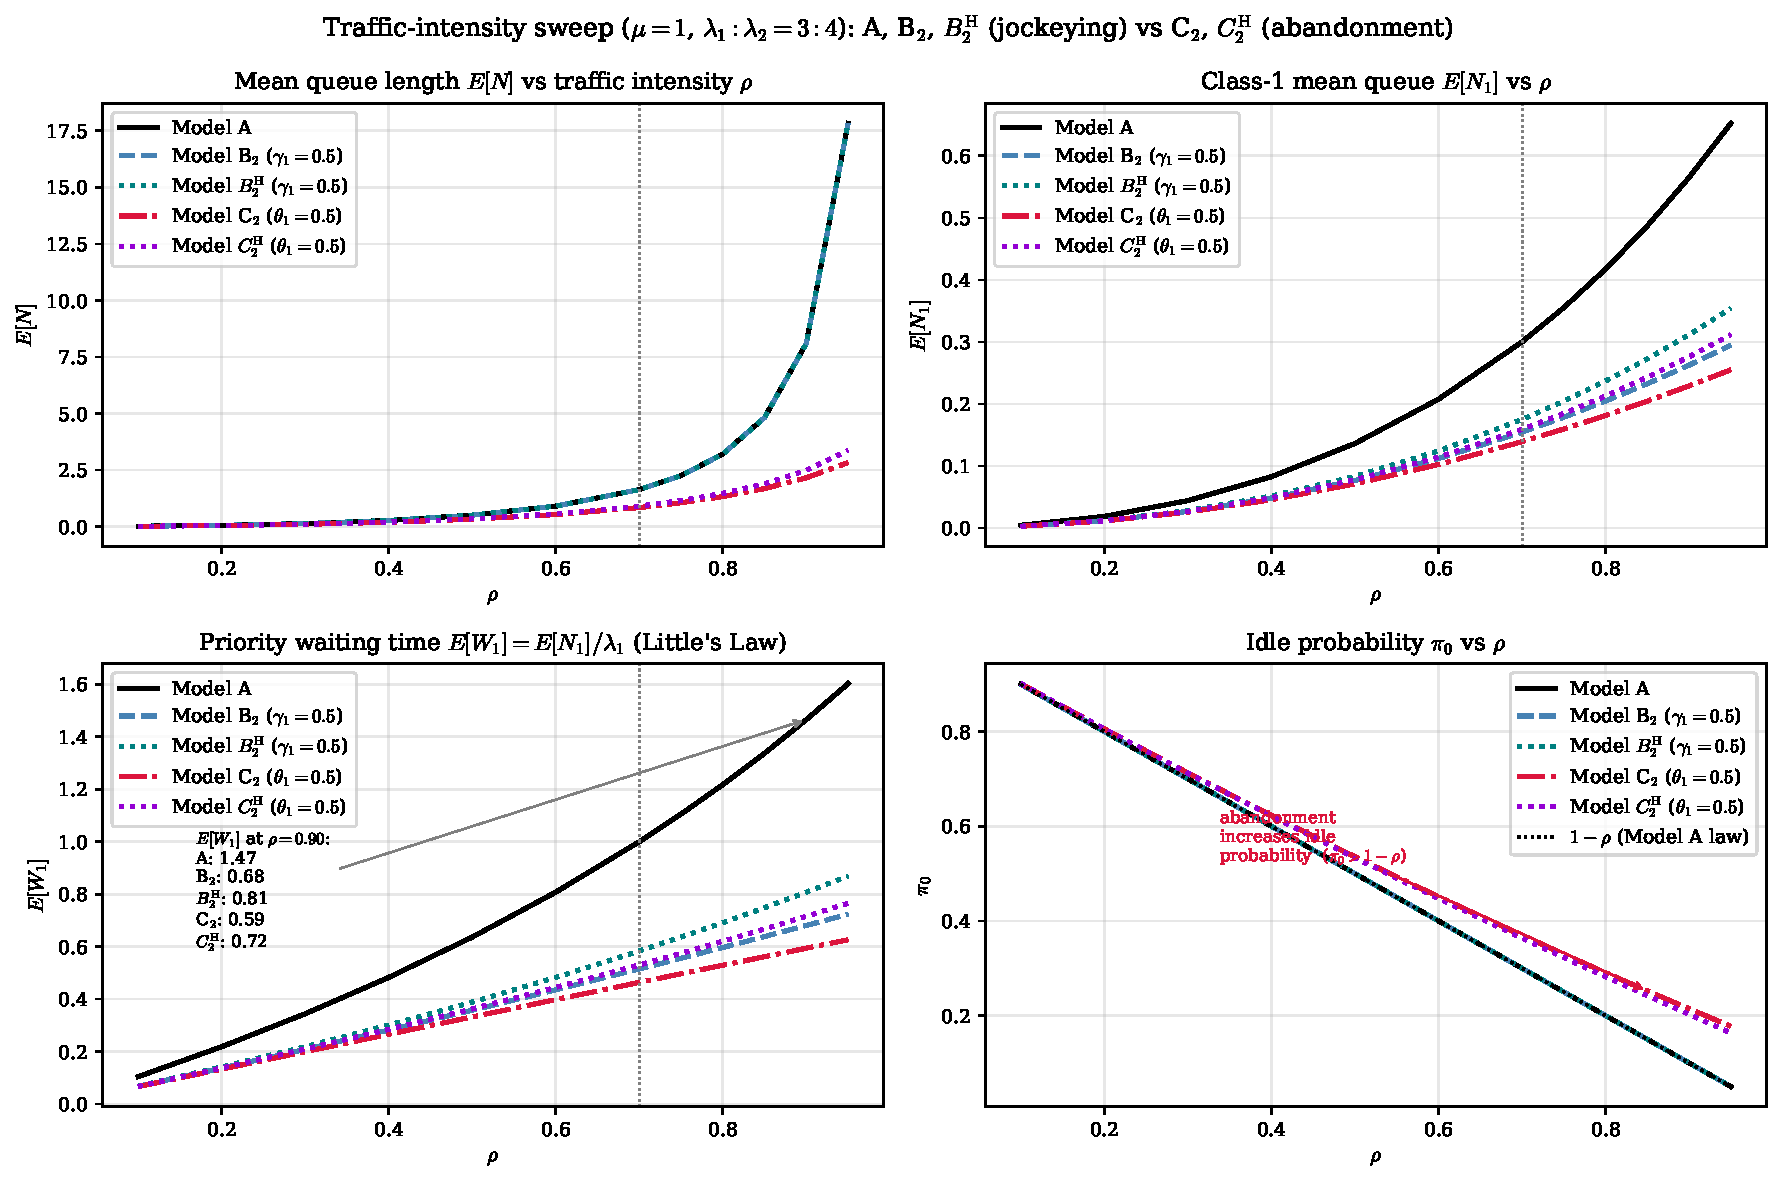
\includegraphics[width=0.98\textwidth]{figures/results/fig_sweep_EN_vs_rho.pdf}
  \caption{Performance versus traffic intensity $\rho$ for the five solved models ---
  the baseline $A$, the jockeying pair $B_2$, $\BH$ ($\gamma_1=0.5$), and the
  abandonment pair $C_2$, $\CH$ ($\theta_1=0.5$) --- at $\mu=1$ and
  $\lambda_1{:}\lambda_2=3{:}4$; the vertical line marks the canonical $\rho=0.70$.
  \emph{Top-left:} total queue $\mathbb{E}[N]$ --- $A$, $B_2$ and $\BH$ coincide because
  jockeying conserves $N$ (Corollaries~\ref{cor:A:pi0}, \ref{cor:B21:pi0}), while $C_2$ and
  $\CH$ lie strictly below because abandonment removes customers ($\CH$ by less).
  \emph{Top-right:} priority queue $\mathbb{E}[N_1]$ --- the head-of-line variants drain it
  less than their full-rate cousins. \emph{Bottom-left:} priority waiting time
  $\mathbb{E}[W_1]$. \emph{Bottom-right:} idle probability $\pi_0$, with the $1-\rho$ law
  (Models~$A$, $B_2$, $\BH$) shown dotted; $C_2$ and $\CH$ sit above it for every $\rho$,
  as predicted by Corollaries~\ref{cor:C2:pi00}, \ref{cor:C21:pi0}.}
  \label{fig:comp:sweep_en}
\end{figure}
%% END SIMULATION RESULTS — fig_sweep_EN_vs_rho %%

%% BEGIN SIMULATION RESULTS — tab_comparison_main %%
\begin{table}[t]\centering
\caption{Comparison of Models $A$, $B$ ($\gamma_1=0.5$, $\gamma_2=0.3$), $B_2$ and $\BH$ ($\gamma_1=0.5$), and $C_2$ and $\CH$ ($\theta_1=0.5$) at three traffic intensities with $\lambda_1{:}\lambda_2=3{:}4$, $\mu=1$. The head-of-line models $\BH$ and $\CH$ use the rate $\gamma_1\mathbf{1}_{\{n_1\geq1\}}$, respectively $\theta_1\mathbf{1}_{\{n_1\geq1\}}$; Model-$B_2$ and Model-$C_2$ use the full rates $\gamma_1 n_1$ and $\theta_1 n_1$. Model-$B$, whose PGF remains open, joins through its truncated-CTMC solution ---like every entry of this table--- since no closed form is required for the comparison.}
\label{tab:comp:main}
\begin{tabular}{llrrrrrrr}
\toprule
$\rho$ & Model & $E[N_1]$ & $E[N_2]$ & $E[N]$ & $E[W_1]$ & $E[W_2]$ & $\pi_0$ & $\pi(0,0)$ \\
\midrule
\multirow{6}{*}{0.50} & $A$ & 0.1364 & 0.3636 & 0.5000 & 0.6364 & 1.2727 & 0.5000 & 0.2500 \\
 & $B$ & 0.1665 & 0.3335 & 0.5000 & 0.7772 & 1.1671 & 0.5000 & 0.2500 \\
 & $B_2$ & 0.0767 & 0.4233 & 0.5000 & 0.3578 & 1.4817 & 0.5000 & 0.2500 \\
 & $\BH$ & 0.0833 & 0.4167 & 0.5000 & 0.3889 & 1.4583 & 0.5000 & 0.2500 \\
 & $C_2$ & 0.0712 & 0.2521 & 0.3233 & 0.3323 & 0.8823 & 0.5356 & 0.2678 \\
 & $\CH$ & 0.0778 & 0.2593 & 0.3370 & 0.3630 & 0.9074 & 0.5333 & 0.2667 \\
\midrule
\multirow{6}{*}{0.70} & $A$ & 0.3000 & 1.3333 & 1.6333 & 1.0000 & 3.3333 & 0.3000 & 0.2100 \\
 & $B$ & 0.5149 & 1.1184 & 1.6333 & 1.7164 & 2.7961 & 0.3000 & 0.2100 \\
 & $B_2$ & 0.1545 & 1.4788 & 1.6333 & 0.5151 & 3.6970 & 0.3000 & 0.2100 \\
 & $\BH$ & 0.1750 & 1.4583 & 1.6333 & 0.5833 & 3.6458 & 0.3000 & 0.2100 \\
 & $C_2$ & 0.1392 & 0.6967 & 0.8358 & 0.4639 & 1.7417 & 0.3696 & 0.2587 \\
 & $\CH$ & 0.1591 & 0.7424 & 0.9015 & 0.5303 & 1.8561 & 0.3636 & 0.2545 \\
\midrule
\multirow{6}{*}{0.90} & $A$ & 0.5651 & 7.5346 & 8.0997 & 1.4651 & 14.6506 & 0.1000 & 0.0900 \\
 & $B$ & 2.6711 & 5.4289 & 8.1000 & 6.9250 & 10.5563 & 0.1000 & 0.0900 \\
 & $B_2$ & 0.2626 & 7.8371 & 8.0997 & 0.6808 & 15.2388 & 0.1000 & 0.0900 \\
 & $\BH$ & 0.3115 & 7.7882 & 8.0997 & 0.8077 & 15.1437 & 0.1000 & 0.0900 \\
 & $C_2$ & 0.2292 & 1.9245 & 2.1537 & 0.5941 & 3.7421 & 0.2146 & 0.1931 \\
 & $\CH$ & 0.2760 & 2.2084 & 2.4844 & 0.7157 & 4.2941 & 0.2025 & 0.1823 \\
\bottomrule
\end{tabular}
\end{table}

%% END SIMULATION RESULTS — tab_comparison_main %%

The two mechanisms produce two qualitatively different responses. Jockeying is internal: the
$1\!\to\!2$ transition relabels a waiting customer without changing the total count. The
$B_2$ and $A$ curves for $\mathbb{E}[N]$ and $\pi_0$ are therefore indistinguishable across the entire
sweep --- the server sees the same workload, and the busy-but-empty probability stays on the
$\rho(1-\rho)$ parabola of Corollary~\ref{cor:B2:pi00}. Abandonment is a true departure at
rate $\theta_1 n_1$, so $C_2$ carries a strictly lighter queue and a strictly larger idle
fraction: the priority backlog is bled off before it can be served. At $\rho=0.70$
(Table~\ref{tab:comp:main}) this gives $\pi_0=\piZeroCtwoSeventy$ for $C_2$ against $\piZeroASeventy$ for $A$ and
$B_2$, and $\mathbb{E}[N]=\ENCtwoSeventy$ against $\ENASeventy$. The divergence widens with load: at
$\rho=0.90$ the baseline class-2 queue reaches $\mathbb{E}[N_2]=\ENtwoANinety$, whereas $C_2$ holds
it to $\ENtwoCtwoNinety$ --- a factor of nearly four. The self-regulating valve $\theta_1 n_1$
acts most strongly precisely when the queue is long. The two head-of-line variants interpolate
monotonically between Model-$A$ and their full-rate parents in every descriptor: $\BH$ conserves
$N$ exactly like $B_2$ and departs only in the $\mathbb{E}[N_1]$ split, while $\CH$ sheds less
load than $C_2$ ($\pi_0=\piZeroCHSeventy$, $\mathbb{E}[N]=\ENCHSeventy$ at $\rho=0.70$).

Two columns warrant a reviewer's caution. First, $\mathbb{E}[W_1]$ is smallest for $C_2$ at
every load, but $\mathbb{E}[W_i]=\mathbb{E}[N_i]/\lambda_i$ counts residence in queue~$i$, which
every departure mode shortens --- service \emph{and} attrition. A smaller $\mathbb{E}[W_1]$ thus
does not certify faster service. Second, jockeying actively \emph{harms} class~2: at $\rho=0.70$,
$B_2$ raises $\mathbb{E}[W_2]$ to $\EWtwoBtwoSeventy$ from the baseline $\EWtwoASeventy$
($+\EWtwoBtwoInflationSeventy\%$). Finally, near criticality the dense CTMC truncation leaves a
boundary tail mass of order $6\times10^{-4}$ for $A$ and $B_2$ at $\rho=0.95$ (against
$1.5\times10^{-7}$ for $C_2$), so the $\rho\ge0.92$ points for the non-abandoning models are
lower bounds.


% ─────────────────────────────────────────────────────────────────────────────
\subsection{Convergence to the baseline}\label{subsec:results:convergence}

Each specialised model must recover Model-$A$ as its distinguishing parameter vanishes; the
comparison above establishes this algebraically, and the CTMC pipeline confirms it numerically.
Measured in the $L_1$ distance $\lVert\pi-\pi_A\rVert_1$, all four specialised models ---
$B_2$, $C_2$, $\BH$, $\CH$ --- approach the baseline at first order in their distinguishing
parameter, with fitted log--log slopes of $0.85$--$0.93$. For the conserving models $B_2$ and
$\BH$ the empty-state descriptors $\pi_0$ and $\pi(0,0)$ equal their Model-$A$ values
\emph{identically} for every $\gamma_1>0$ (Corollaries~\ref{cor:B2:pi00}, \ref{cor:B21:pi0}),
so the approach is carried entirely by interior redistribution of mass.

\section{Conclusion and Future Work}\label{sec:conclusion}

This thesis analysed a two-class non-preemptive priority $M/M/1$ queue under two waiting-room mechanisms ---jockeying and abandonment. It obtained the exact stationary bivariate PGF $P(x,y)$ in closed or integral form for five models: the baseline Model-$A$, one-way ($1\to2$) jockeying Model-$B_2$, class-$1$ abandonment Model-$C_2$, and the head-of-line variants Model-$\BH$ and Model-$\CH$.

One common property is shared by all solved models: the form of the fundamental equation that the PGF satisfies ---algebraic, or carrying derivative terms--- determines the tractability of the model with the methods employed in this work. As a result, the collection of closed-form solutions is smaller than the model hierarchy might suggest: derivative terms in $y$ complicate the problem, as one would need more advanced mathematical tools to determine the boundary function $P_y(y)$.


\subsection{The obstruction and the mechanism dichotomy}



Read as a competition between an algebraic coefficient and two derivative terms, the fundamental equation exposes a clean dichotomy. Where the equation is solvable, the unknown boundary function $P_y(y)$ is determined by exactly one of four mechanisms. The first is evaluation at a kernel root lying strictly inside the unit disc ---the purely algebraic route of the baseline Model-$A$. The second is interior analyticity: when one-way jockeying survives, the factor $(x-y)$ places the operative singularity at the diagonal point $x=y$ inside the disc, and the boundary function is fixed by requiring analyticity there (Model-$B_2$). The third is boundary boundedness: when class-$1$ abandonment survives, the factor $(x-1)$ moves the singularity to the unit-circle boundary $x=1$, where mere boundedness of the PGF suffices to determine the unknown (Model-$C_2$). The fourth is head-of-line algebraic collapse: restricting a mechanism to the head-of-line customer replaces the length-proportional rate with a constant one, eliminates the derivative term in the equation, and recovers the purely algebraic form of Model-$A$, solvable by the same kernel argument (Models~$\BH$ and~$\CH$).

The unsolvable cases ---Model-$B$ and Model-$X$--- make structural limits apparent, as the derivative terms in $y$ make the task of determining $P_y(y)$ significantly more challenging than it already was. Model-$B$ requires solving a Volterra-type integral equation whose forcing term depends on the boundary function itself; Model-$X$ further compounds this difficulty with non-linear characteristic curves, although we have not determined the exact difficulty or feasibility of the problem. The hierarchy is therefore not a loose collection of cases, but a complete enumeration: four mechanisms that enable exact solutions and two obstructions that prevent them.

The two mechanisms themselves act in opposite directions. Jockeying \emph{redistributes} delay at fixed total work: relocating a waiting customer conserves the total count, so $\mathbb{E}[N]$, $\pi_0$ and $\pi(0,0)$ are identical to the baseline for every $\gamma_1$. The mechanism's entire effect is to move delay between classes ---the priority premium $\mathbb{E}[W_2]/\mathbb{E}[W_1]$ inflating to $\premiumBtwoNinety$ at $\rho=0.90$ against the Model-$A$ value $\premiumANinety$.

Abandonment instead \emph{reduces} the load: the idle probability rises, every queue shortens, and total waiting times fall.

\subsection{Limitations}

Several assumptions are intrinsic to the $M/M/1$ framework itself. All results rest on exponential interarrival, service, jockeying, and abandonment times ---an idealisation that is most restrictive for the service times. Allowing class-dependent rates $\mu_1 \neq \mu_2$ would invalidate the analysis at its foundation, since the state-space construction and the definition of the limiting probabilities both rely on the server being indifferent to the class in service. Relaxing exponentiality entirely to general service times further compounds the difficulty; the intractability that already forces de~Waal's approximate $M/G/1$ treatment illustrates how quickly the problem ceases to admit closed-form solutions.

The partial-PGF result on the alternative state space $\widetilde{S}$ is an approximation, not a theorem, and should be read as a documented negative result. The rationale was as follows. Cohen~\cite{cohen1956delay} applied a partial generating function on the standard state space $(n_1,n_2)$ with respect to the class-2 variable, leaving the tractable class-1 subsystem untouched and transforming only in the harder direction. In the presence of jockeying, neither class has simple dynamics individually, but the total queue length $N = N_1 + N_2$ does. The alternative state space $(n_2, n)$ was therefore introduced to exploit this total-count structure. The attempt does not succeed: rather than simplifying the problem, the change of coordinates makes the balance equations harder even for Model-$A$.

\subsection{Future work}\label{sec:future_work}

Several extensions follow directly from the mathematical machinery used:
\begin{enumerate}
  \item \emph{Head-of-line versions of the remaining models.} The head-of-line models could be extended with bidirectional active mechanisms ---namely Model-$B^\mathrm{H}$ for jockeying and Model-$C^\mathrm{H}$ for abandonment--- rather than limiting them to strictly one direction, as the derivative terms in the fundamental equation would also disappear. Even a head-of-line model carrying both active mechanisms at the same time, Model-$X^\mathrm{H}$, would remain algebraic. These extensions appear to be within reach of the tools already developed here.
  \item \emph{The $k$-customer head-of-line ladder.} The head-of-line variants let only the single customer at the head of the queue for class~$1$ jockey or abandon; the natural extension lets the first $k$ waiting class-$1$ customers do so, jockeying at rate $\gamma_1\min(n_1,k)$ (and likewise abandoning at rate $\theta_1\min(n_1,k)$). Writing $\min(n_1,k)=\sum_{j=1}^{k}\mathbf 1_{\{n_1\ge j\}}$, the bounded rate keeps the fundamental equation \emph{algebraic} at the potential price of $k$ unknown boundary functions. This route has not been explored in this work, so it is unclear what it could yield. One would expect that such models would converge to Model-$B_2$ and Model-$C_2$ as $k\to\infty$.
  \item \emph{Numerical solution of the Model-$B$ Volterra equation.} Unlike Model-$X$, Model-$B$ yields a first-kind Volterra equation with an \emph{explicit} kernel and a \emph{known} forcing term. Whether its solution can be characterised further ---in closed form or through numerical approximation--- is left open; either route lies beyond the scope of this thesis.
  \item \emph{Multi-server extension.} Carrying the mechanisms to $M/M/c$ would connect this single-server line to the multi-server setting. With a common service rate for both classes, the non-preemptive priority $M/M/c$ queue admits an exact waiting-time analysis~\cite{kella1985waiting}, and exact methodology for two priority classes exists even with class-dependent rates under a preemptive discipline~\cite{wang2015mmc}, so exactness need not be surrendered at the outset; the open question is whether jockeying and abandonment can be added while preserving it. This would also connect to the (approximate) proactive-scheduling results of~\cite{huchandong2022proactive}.
  \item \emph{Derive mean performance metrics.} The closed-form PGFs obtained for Model-$B_2$, Model-$C_2$, Model-$\BH$, and Model-$\CH$ contain the full distributional information, but extracting mean queue lengths and waiting times requires differentiating at $(1,1)$, which in Model-$B_2$ and Model-$C_2$ involves boundary functions given as integrals. A systematic differentiation ---applying L'H\^opital where necessary at the singularity $x=1$--- would yield closed-form expressions for $\mathbb{E}[N_1]$, $\mathbb{E}[N_2]$, and, via Little's law, $\mathbb{E}[W_1]$ and $\mathbb{E}[W_2]$, replacing the numerical estimates reported in the results chapter with exact ones.
  \item \emph{Calibration.} Fitting $\gamma_1$, $\theta_1$ and the loads to real elderly-care waiting-list data~\cite{zenios1999modeling} would test whether the regimes identified here accurately describe operational reality. Since the transplant waiting-list model of~\cite{zenios1999modeling} differs from ours in several respects, such a calibration would likely require further model extensions rather than a direct fit of $\gamma_1$ and $\theta_1$.
\end{enumerate}


\appendix
\section{Extended numerical verification and comparison}\label{app:numerics}

This appendix collects the full figure-by-figure evidence summarised in
Section~\ref{sec:results}: the per-result verification maps, the simulation cross-checks, the
extended traffic-intensity and mechanism sweeps, the class-asymmetry study, the convergence
diagnostics, and the synoptic dashboard. Unless stated otherwise all figures use the base
parameters of Section~\ref{sec:results} --- $\lambda_1=0.3$, $\lambda_2=0.4$, $\mu=1.0$, with
the mechanism parameter ($\gamma_1$ or $\theta_1$) set to $0.5$ where applicable --- and the
truncated CTMC ($N_{\max}=40$) as ground truth.

% =====================================================================
\subsection{Verification against the CTMC}\label{app:numerics:validation}

These figures provide the visual evidence behind the verdicts of
Table~\ref{tab:validation_summary}.

\subsubsection*{Structural lemmas}

The lemmas assert that the stationary distribution satisfies a specific
functional equation, so a non-vanishing residual would indicate either a
derivation error in the lemma or a coding error in the solver.
Figure~\ref{fig:val_lemmas} shows the maximum relative residual
$|{\rm LHS}-{\rm RHS}|/|{\rm RHS}|$ of each lemma's functional equation,
evaluated on the exact CTMC distribution across all model variants.
Both lemmas hold to better than $10^{-9}$ --- consistent with truncation noise at
$N_{\max}=40$, not formula error --- and Lemma~\ref{lem:gen:PPGF_dynamics} reaches floating-point
precision (${\sim}10^{-15}$) because its recurrence involves only one
discrete variable.

\begin{figure}[H]
    \centering
    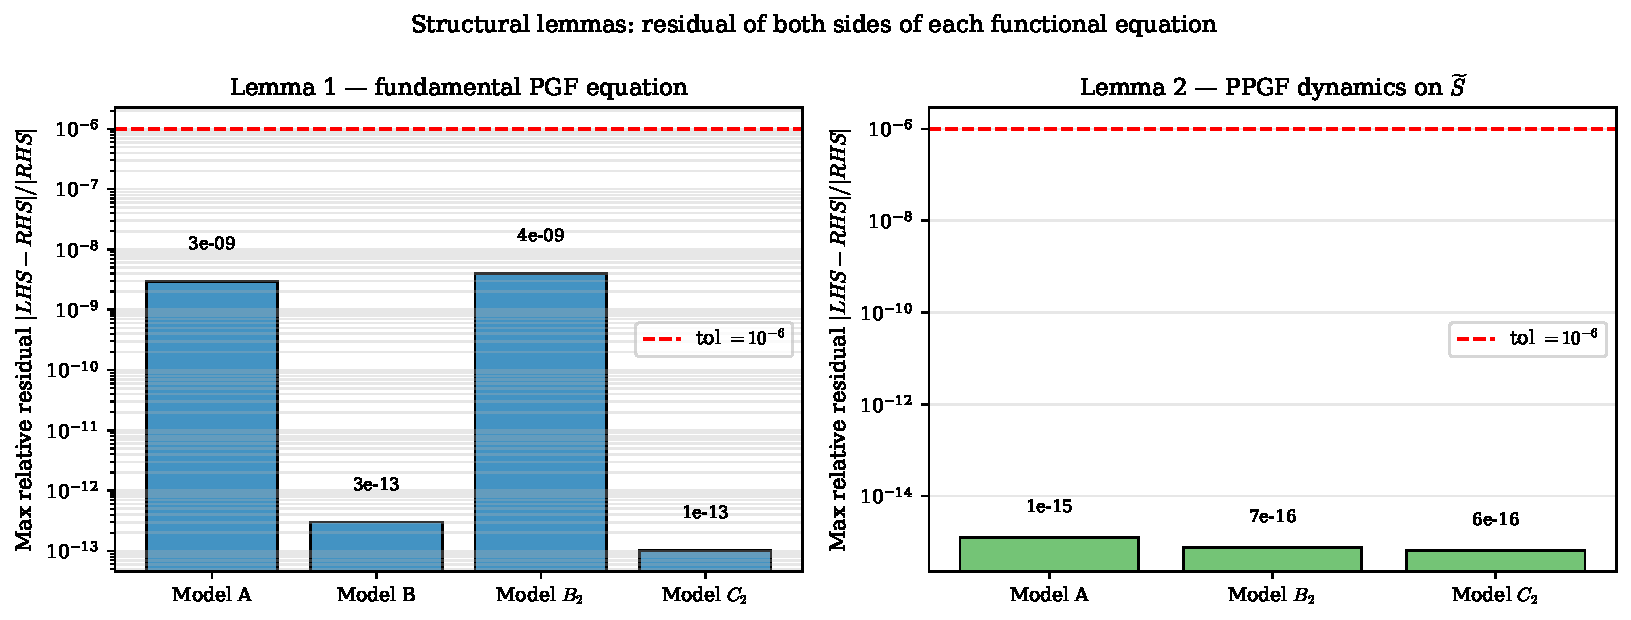
\includegraphics[width=0.90\textwidth]{figures/validation/val_lemmas.pdf}
    \caption{Lemma verification.  \textit{Left}: max relative residual of the
    fundamental PGF equation (Lemma~\ref{lem:gen:fundamental_equation}) for
    each model variant on a $5\times5$ interior grid.
    \textit{Right}: max relative residual of the PPGF dynamics recurrence
    (Lemma~\ref{lem:gen:PPGF_dynamics}) over $n\in\{1,\ldots,15\}$ and
    $y\in[0.05,0.90]$.
    All values lie well below the $10^{-6}$ tolerance (red dashed line).}
    \label{fig:val_lemmas}
\end{figure}

\subsubsection*{Closed-form and integral-form theorems}

Figures~\ref{fig:val_pxy} and~\ref{fig:val_py} compare the three analytic
formulas against the CTMC on a uniform grid, using identical parameters and
the same error metric; since only the extra mechanism changes between panels,
the errors are directly comparable. Model-$C_2$ reaches near-machine precision
because its closed form evaluates exactly through the Pollaczek--Khinchine
ratio; Model-$B_2$'s accuracy (${\sim}10^{-7}$) is limited instead by the
numerical quadrature of its integral representation, whose integrand steepens
near the branch point at $x=y$.

\begin{figure}[H]
    \centering
    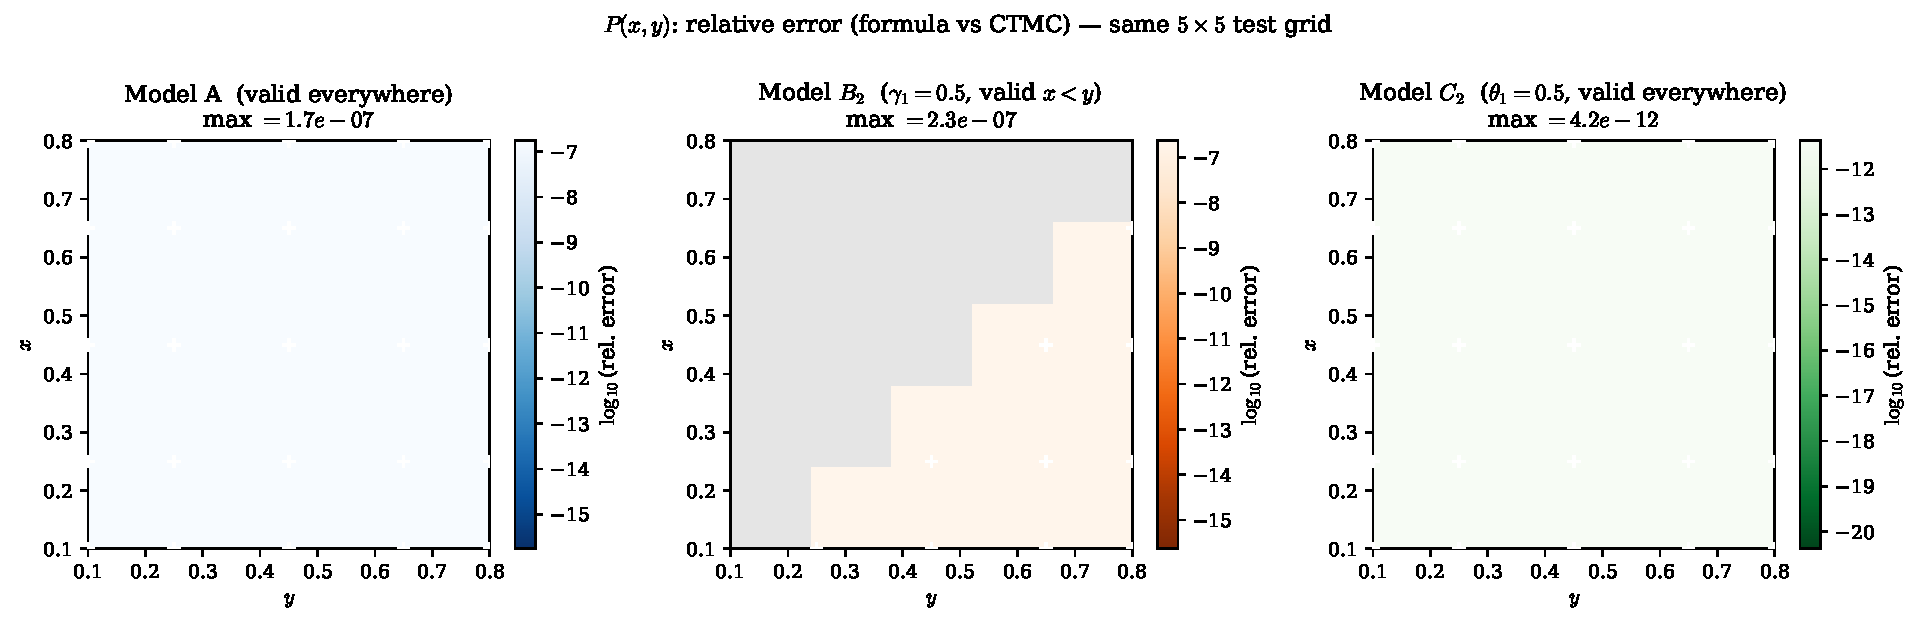
\includegraphics[width=\textwidth]{figures/validation/val_theorems_pxy.pdf}
    \caption{Relative error $|P_{\rm formula}(x,y)-P_{\rm CTMC}(x,y)|/|P_{\rm CTMC}(x,y)|$
    on the same $5\times5$ test grid for Models $A$, B$_2$, and C$_2$.
    Colour scales are anchored to the same range across all three panels.
    White crosses mark the 25 test points.}
    \label{fig:val_pxy}
\end{figure}

\begin{figure}[H]
    \centering
    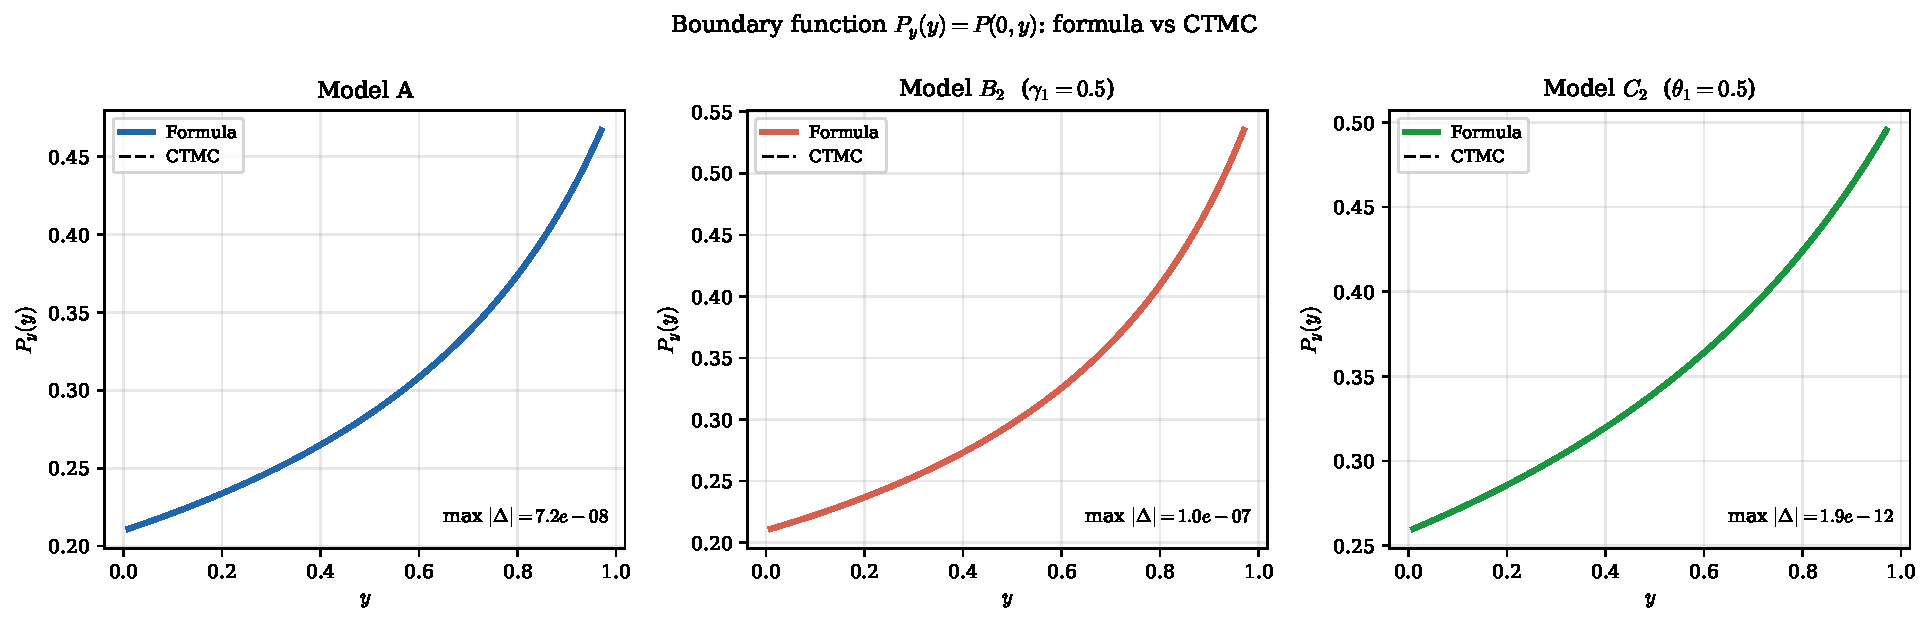
\includegraphics[width=\textwidth]{figures/validation/val_theorems_py.pdf}
    \caption{Boundary function $P_y(y)=P(0,y)$ for Models $A$, B$_2$, and C$_2$:
    analytic formula (solid) vs CTMC (dashed). All three curves rise
    monotonically to $P(0,1)$, the probability that the server is busy with an
    empty priority queue, but their levels differ: each mechanism changes how
    class-1 customers block class-2 service.}
    \label{fig:val_py}
\end{figure}

\subsubsection*{Corollaries}

The two corollaries are structurally very different: for the conserving models
($A$, $B$, $B_2$) the empty-state probabilities depend on the parameters only
through the total load $\rho$, whereas the Model-$C_2$ expressions run through
the busy-period mean $\mathbb{E}[B_C]$ and hence the confluent hypergeometric
function. Both are tested identically.
Figure~\ref{fig:val_corollaries} shows the scatter of formula vs CTMC values
for $\pi_0$ and $\pi(0,0)$ across 60 random parameter configurations for each
corollary.  All points lie on the diagonal to within $10^{-4}$.

\begin{figure}[H]
    \centering
    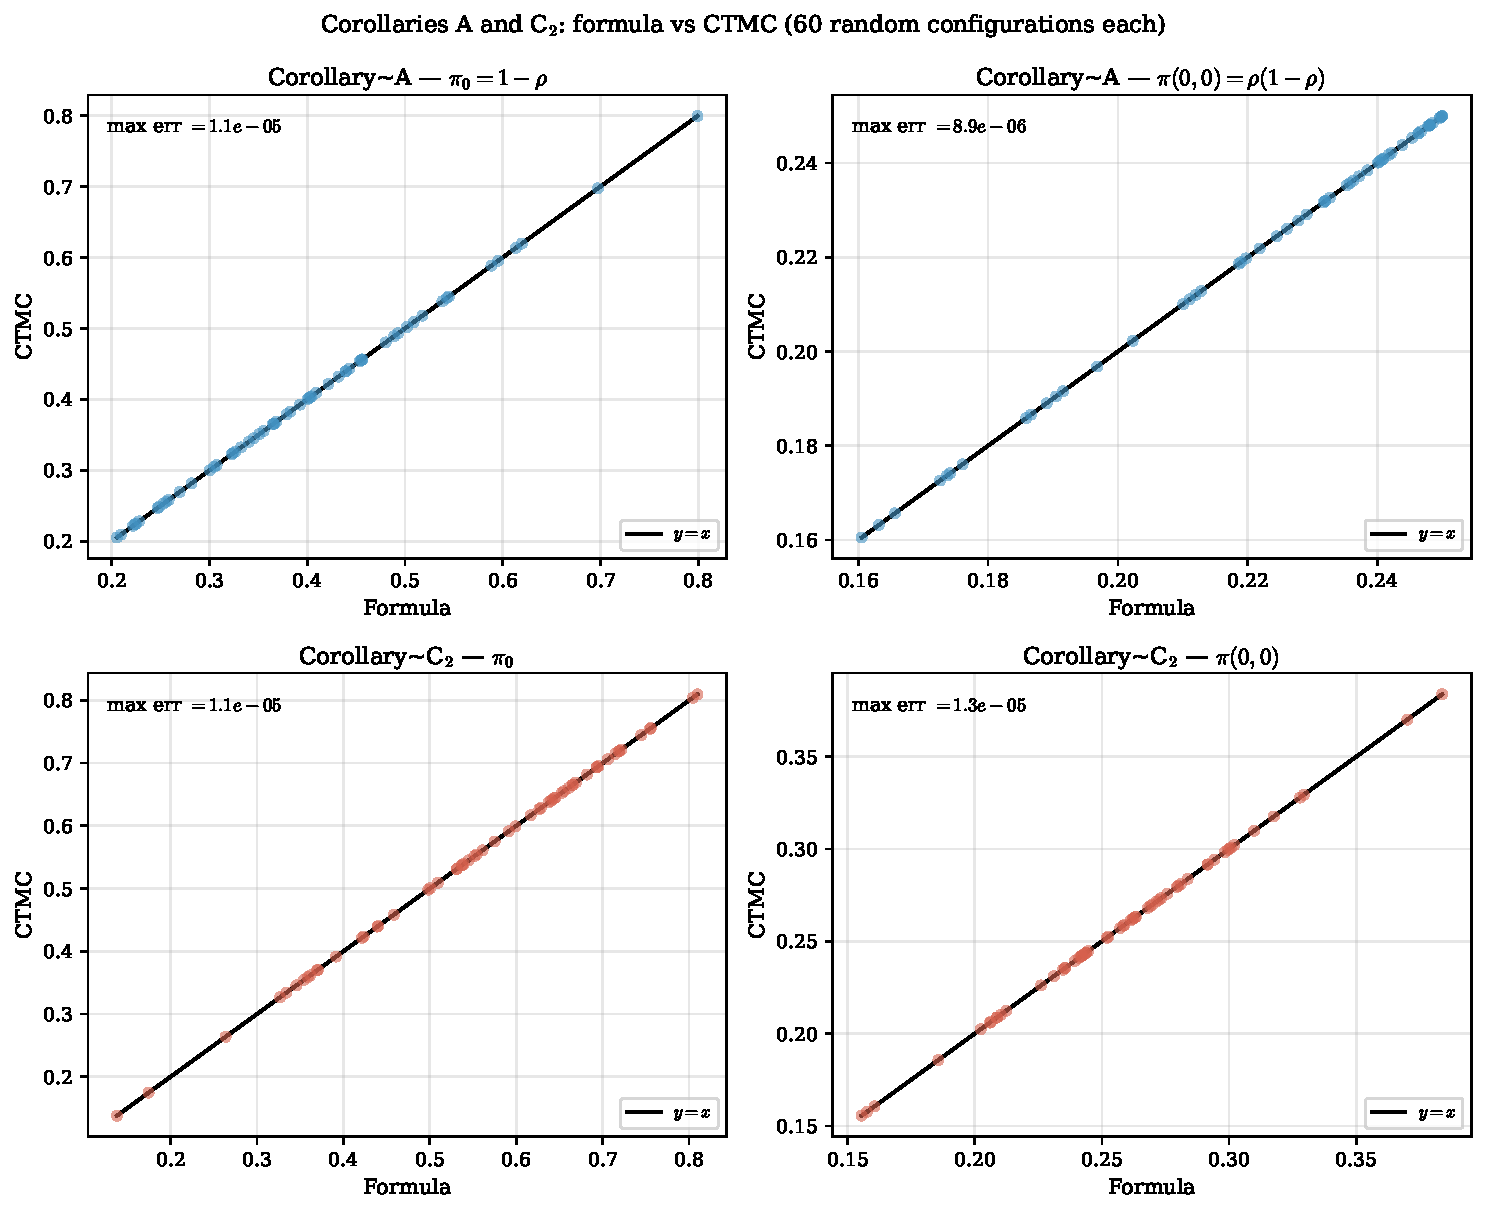
\includegraphics[width=0.80\textwidth]{figures/validation/val_corollaries.pdf}
    \caption{Corollaries A (blue) and C$_2$ (red): formula vs CTMC for
    $\pi_0$ (left column) and $\pi(0,0)$ (right column) over 60 random
    configurations each.  Perfect agreement lies on the diagonal. The C$_2$
    corollary, despite running through the $M/M/1+M$ busy period and the
    confluent hypergeometric function, matches the CTMC to the same tolerance
    as the rational Model-$A$ formula.}
    \label{fig:val_corollaries}
\end{figure}

\subsubsection*{PPGF approximation (Approximation~\ref{apx:A:PPGF_Stilde})}

Unlike the exact results of Table~\ref{tab:validation_summary}, this result is
approximate by design: the recursion drops the boundary-diagonal forcing term,
which decays geometrically in $n$, so the approximation is exact at $y=1$ for
all parameters but degrades wherever the neglected forcing competes with the
homogeneous solution. Figure~\ref{fig:val_ppgf} maps the maximum relative error
$\varepsilon_\infty(\rho_1,\rho_2)$ over the parameter space and confirms the
validity region characterised in \S\ref{ssec:A:Stilde}: the priority-dominated,
moderately loaded regime. This is the single conditionally accepted result of the
verification exercise ---assessed separately from Table~\ref{tab:validation_summary}---
and the one place where the alternative coordinatisation
$\widetilde{S}$ does not yield an exact result.

\begin{figure}[H]
    \centering
    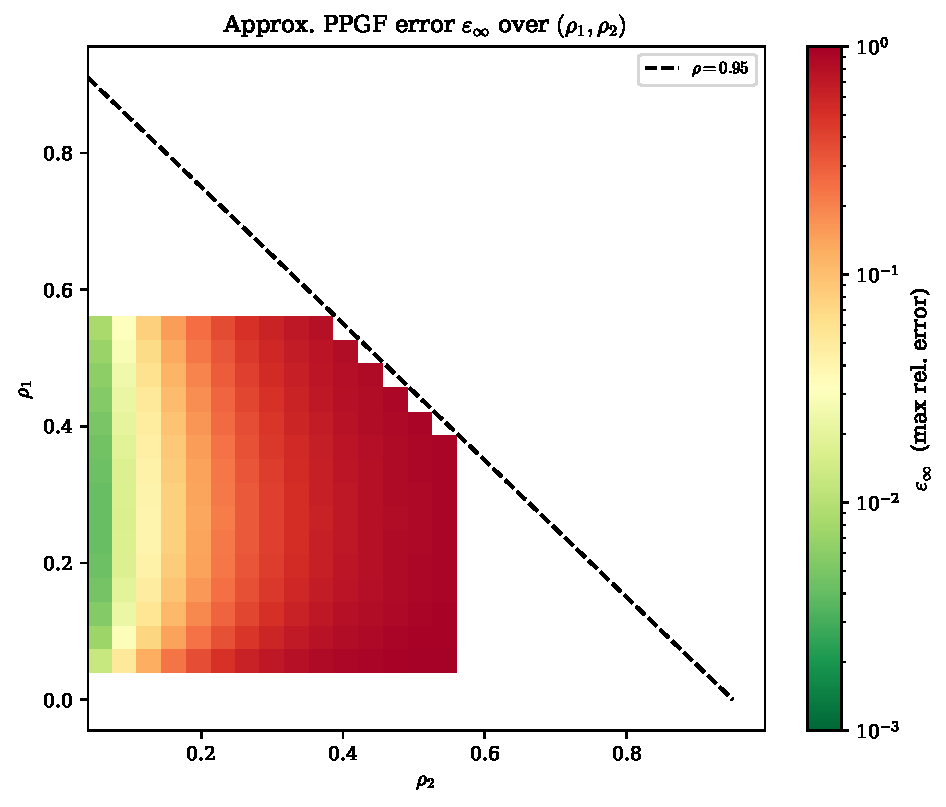
\includegraphics[width=0.52\textwidth]{figures/validation/val_ppgf_heatmap.pdf}
    \caption{Max relative error $\varepsilon_\infty$ of the approximate PPGF
    $\widetilde{P}_{\rm app}(y,n)=(1-\rho)\rho[\widetilde{y}^*(y)]^n$ as a
    function of $(\rho_1,\rho_2)$.
    \emph{Colour convention} (shared with the $\mathbb{E}[N_1]$ heatmap,
    Figure~\ref{fig:c2:heatmap}): \textcolor{green!60!black}{green} marks the
    accurate regime ($\varepsilon_\infty<3\%$) and \textcolor{red}{red} the
    inaccurate one---green favourable, red unfavourable, in the same direction
    across both maps.
    The approximation is reliable only when the priority class carries most
    of the offered load ($\rho_1/\rho\gtrsim0.6$) and the system is not
    heavily loaded ($\rho\lesssim0.6$).}
    \label{fig:val_ppgf}
\end{figure}

\subsubsection*{Head-of-line models \texorpdfstring{$\BH$}{B2-H} and \texorpdfstring{$\CH$}{C2-H}}

The two head-of-line models possess algebraic fundamental equations.  The lemma
check therefore requires no differentiation of $P$: only the CTMC values of
$P(x,y)$ and $P_y(y)$ are substituted into each side and the residual is
measured. The theorem check is the same $P(x,y)$ grid comparison used for
Models~$A$, $B_2$, and $C_2$. Figure~\ref{fig:val_experiment} reports both checks, and
Figure~\ref{fig:val_experiment_pi} tracks the empty-state probabilities $\pi_0$
and $\pi(0,0)$ as the mechanism parameter grows.

\begin{figure}[H]
    \centering
    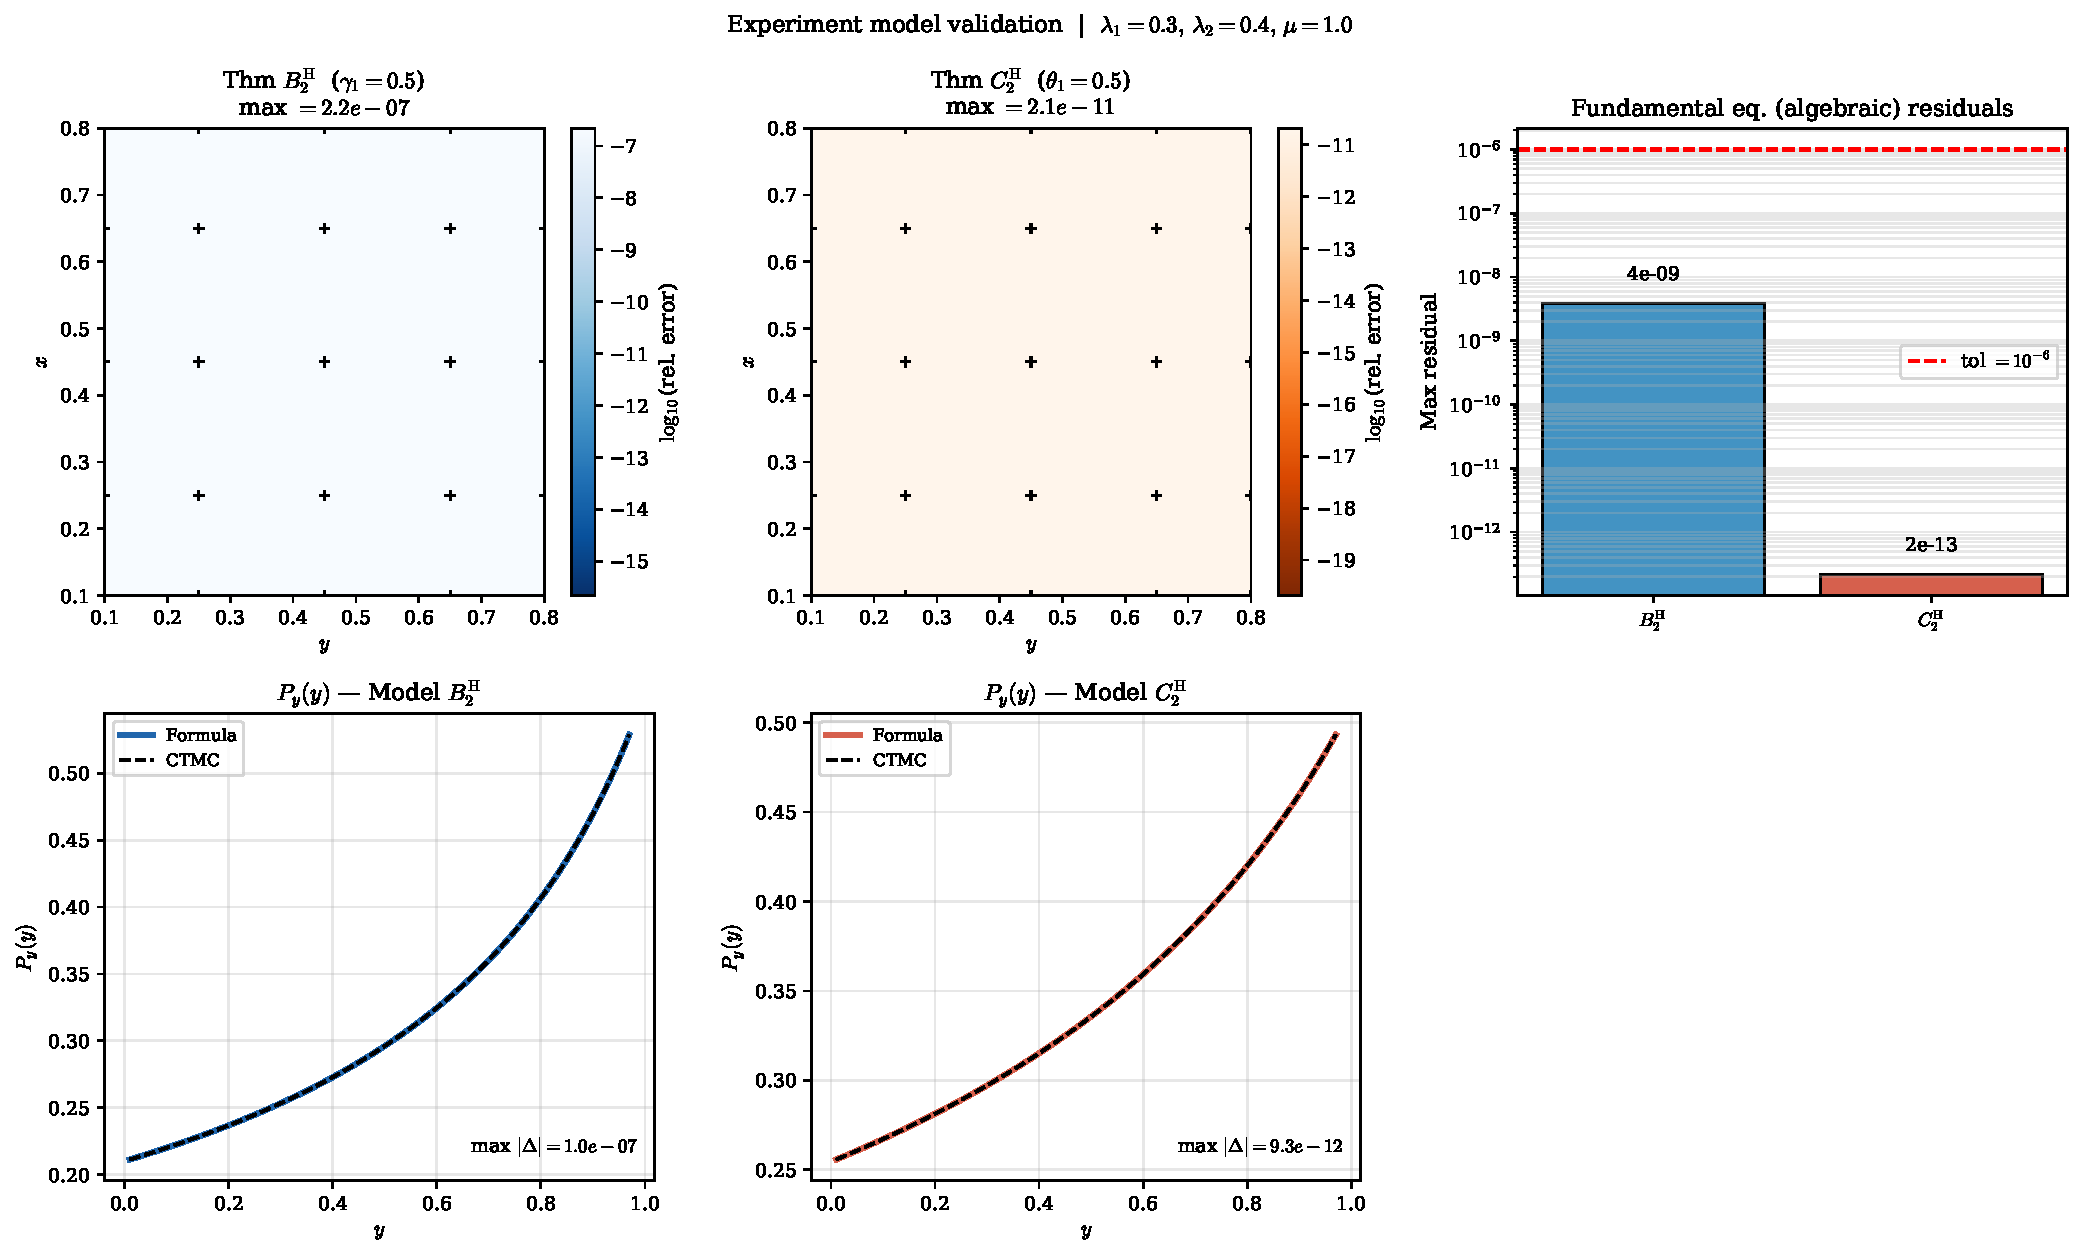
\includegraphics[width=\textwidth]{figures/validation/val_experiment.pdf}
    \caption{Verification of Models $\BH$ and $\CH$.
    \textit{Top row, left and centre}: relative error
    $|P_{\rm formula}(x,y)-P_{\rm CTMC}(x,y)|/|P_{\rm CTMC}(x,y)|$
    on the 5$\times$5 test grid.
    \textit{Top row, right}: maximum relative residual of the algebraic
    fundamental equation for each model — both well below the $10^{-6}$
    tolerance.
    \textit{Bottom row}: boundary function $P_y(y)=P(0,y)$ comparing the
    rational closed-form formula against the CTMC.
    $\BH$ matches the Model-$A$ accuracy (${\sim}10^{-7}$), while $\CH$
    reaches near-machine precision (${\sim}10^{-11}$) because the denominator
    of its rational formula stays well away from zero over the test range;
    both lemma residuals lie far below the $10^{-6}$ tolerance, confirming the
    algebraic derivation.}
    \label{fig:val_experiment}
\end{figure}

\begin{figure}[H]
    \centering
    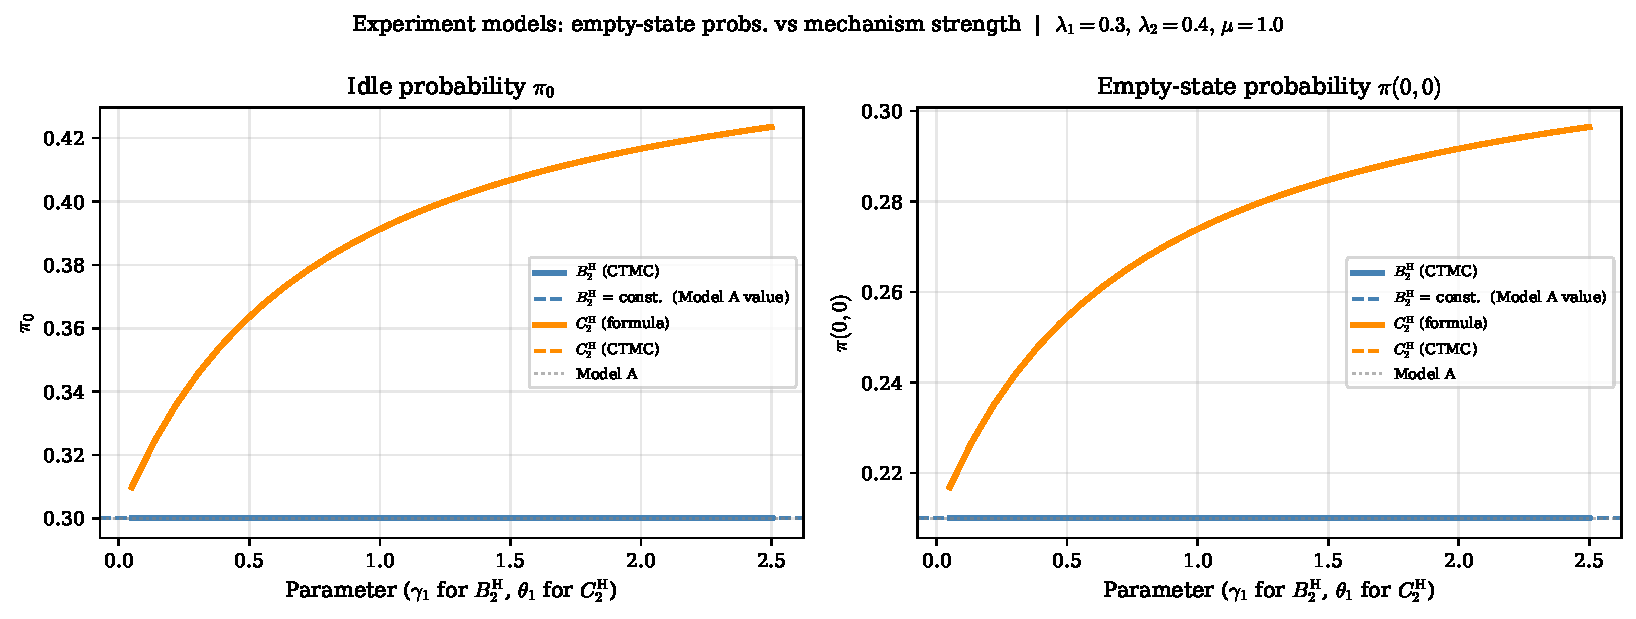
\includegraphics[width=0.85\textwidth]{figures/validation/val_experiment_pi.pdf}
    \caption{Empty-state probabilities $\pi_0$ and $\pi(0,0)$ as the mechanism
    parameter increases from $0$ to $2.5$.
    \textit{Left}: $\BH$ (blue) maintains $\pi_0=1-\rho$ exactly for all
    $\gamma_1$ — jockeying conserves total customers.
    $\CH$ (orange) shows $\pi_0$ increasing with $\theta_1$: abandonment
    clears the priority queue faster, raising the server's idle fraction.
    \textit{Right}: same story for $\pi(0,0)$.
    Solid orange = closed-form formula~\eqref{eq:C21:pi0_pi00}; dashed orange
    = CTMC.  The two are indistinguishable (max error $<10^{-4}$).
    The flat $\BH$ line is a structural result, not merely a numerical
    observation: $\pi_0=1-\rho$ holds identically for every $\gamma_1$ by the
    conservation corollary.}
    \label{fig:val_experiment_pi}
\end{figure}

\subsubsection{Cross-verification: simulation versus the CTMC}
\label{subsec:results:crossval}

The CTMC solver is the analytical ground truth used throughout this work, but it is
itself a numerical object: it solves $\pi Q=0$ on a finite truncation of the state space.
As an independent check, the stationary distribution is also estimated by a discrete-event
simulation of the master Markov chain, driven by the same rate structure but making no
truncation and no linear-algebra assumption. Figure~\ref{fig:results:crossval} plots, for
each canonical model, the CTMC value $\pi(n_1,n_2)$ against the simulated frequency for
every state with $\pi(n_1,n_2)>10^{-4}$.

%% BEGIN SIMULATION RESULTS — fig_sim_vs_ctmc %%
\begin{figure}[H]
  \centering
  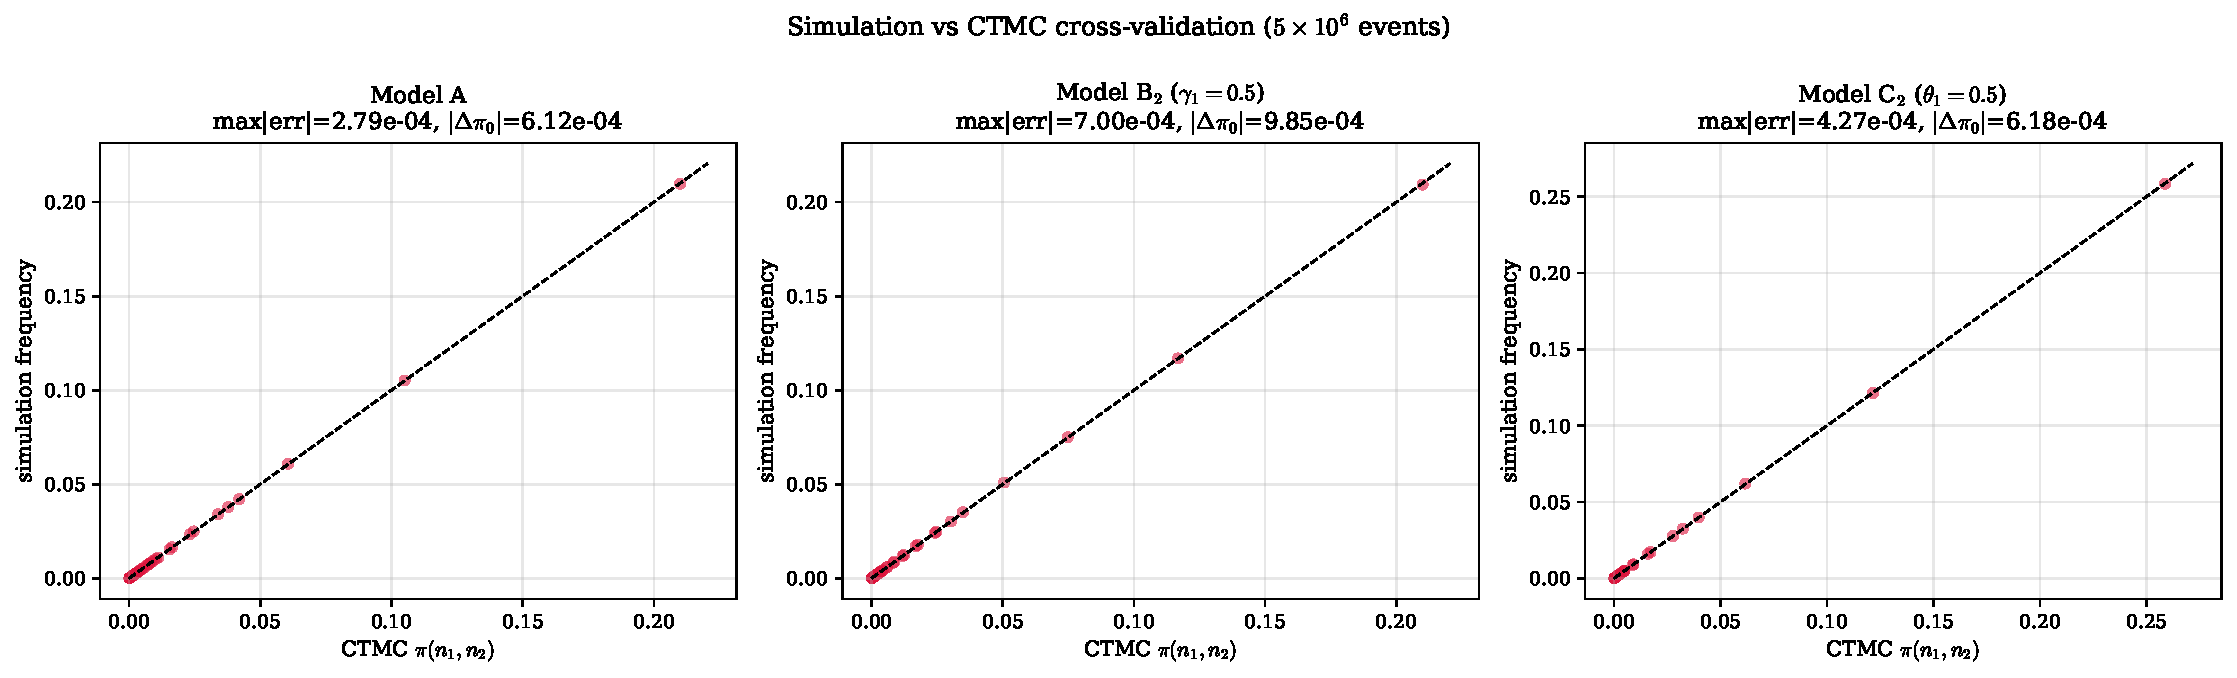
\includegraphics[width=0.98\textwidth]{figures/results/fig_sim_vs_ctmc.pdf}
  \caption{Simulation versus exact CTMC for Models $A$, $B_2$ ($\gamma_1=0.5$) and $C_2$
  ($\theta_1=0.5$) at $\lambda_1=0.3$, $\lambda_2=0.4$, $\mu=1$. Each point is one state
  $(n_1,n_2)$; the dashed line is $y=x$. The simulation uses $5\times10^6$ events (lower
  precision than the CTMC), yet every point lies on the diagonal, with maximum absolute
  discrepancy below $10^{-2}$ for all three models.}
  \label{fig:results:crossval}
\end{figure}
%% END SIMULATION RESULTS — fig_sim_vs_ctmc %%

The points cluster tightly on the $y=x$ line in all three panels, and the maximum absolute
deviation between the two independent computations is below $10^{-2}$ throughout --- the
residual being entirely consistent with the $O(1/\sqrt{n})$ sampling error of a
$5\times10^6$-event run. The two methods agree on $\pi_0$ to the same order. This closes the
verification loop: the closed-form expressions match the CTMC (\S\ref{subsec:validation} and
Table~\ref{tab:validation_summary}), and the CTMC matches an assumption-free simulation,
so the analytical formulas are verified against a fully independent estimator.

The same cross-check is run for the two head-of-line experiment models, whose CTMC carries a
\emph{constant} class-1 mechanism rate $\gamma_1\mathbf{1}_{\{n_1\ge1\}}$ or
$\theta_1\mathbf{1}_{\{n_1\ge1\}}$ rather than the length-proportional $\gamma_1 n_1$ or
$\theta_1 n_1$ of $B_2$, $C_2$. Both the event-driven simulator and the truncated solver
honour this head-of-line rate, so Figure~\ref{fig:results:crossval_exp} is an independent
test of the new transition structure underlying Models~$\BH$ and~$\CH$.

%% BEGIN SIMULATION RESULTS — fig_sim_vs_ctmc_experiment %%
\begin{figure}[H]
  \centering
  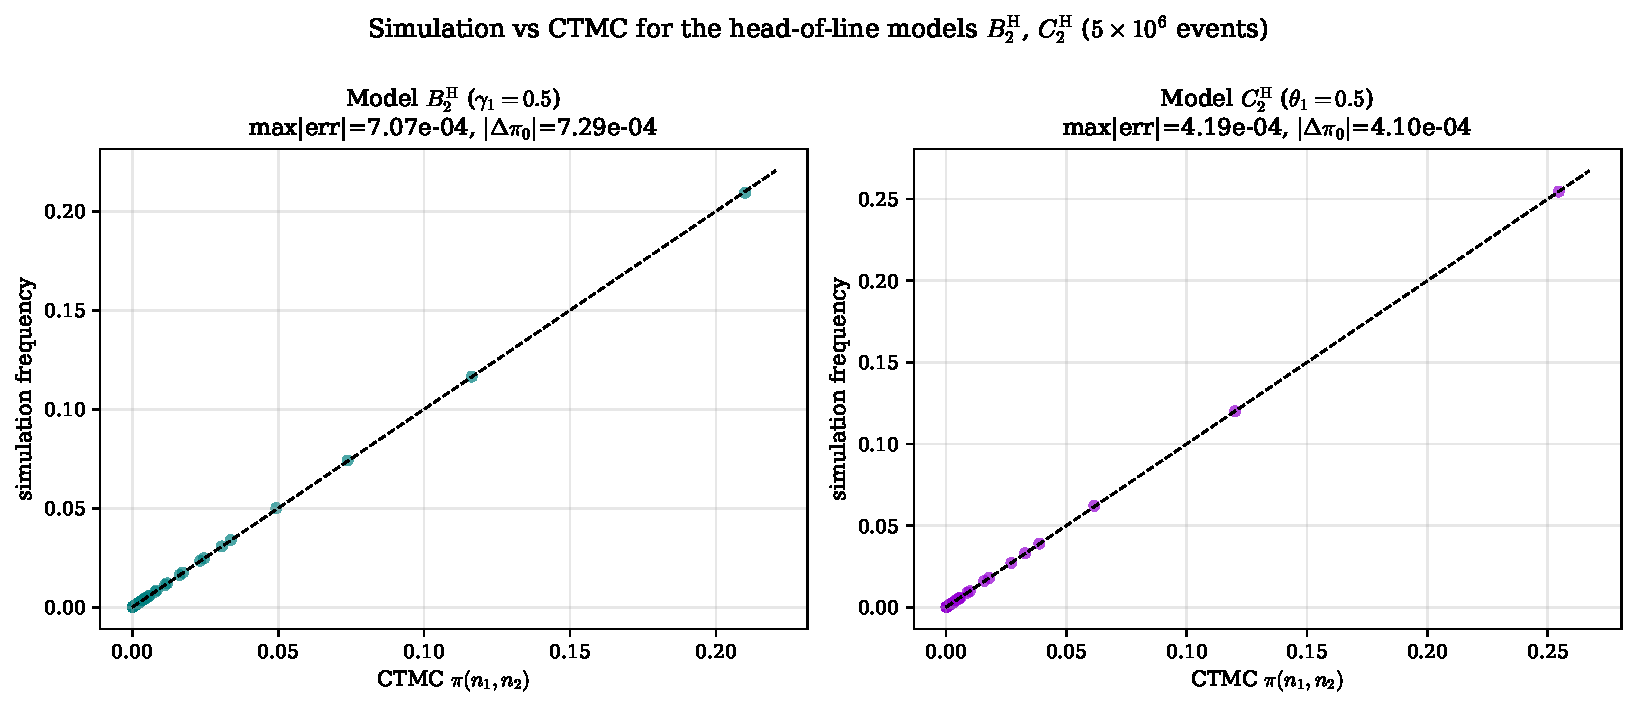
\includegraphics[width=0.82\textwidth]{figures/results/fig_sim_vs_ctmc_experiment.pdf}
  \caption{Simulation versus exact CTMC for the head-of-line models $\BH$
  ($\gamma_1=0.5$) and $\CH$ ($\theta_1=0.5$) at $\lambda_1=0.3$, $\lambda_2=0.4$,
  $\mu=1$. Each point is one state $(n_1,n_2)$; the dashed line is $y=x$. As for the
  full-rate models, every point lies on the diagonal, with maximum absolute discrepancy
  below $10^{-2}$, confirming that the constant-rate $\mathbf{1}_{\{n_1\ge1\}}$ transition is
  implemented consistently in both the simulator and the solver.}
  \label{fig:results:crossval_exp}
\end{figure}
%% END SIMULATION RESULTS — fig_sim_vs_ctmc_experiment %%

% =====================================================================
\subsection{Extended traffic-intensity and mechanism sweeps}\label{app:numerics:sweep}

This subsection expands the quantitative comparison of \S\ref{subsec:comp:sweep}: the
$\pi(0,0)$ sweep, the companion loss-accounting and queue-length tables, the isolated
jockeying and abandonment sweeps, the class-asymmetry study, the priority-benefit contrast,
and the head-of-line versus full-rate comparison.

\subsubsection{The busy-but-empty probability \texorpdfstring{$\pi(0,0)$}{pi(0,0)}}

%% BEGIN SIMULATION RESULTS — fig_sweep_pi00_vs_rho %%
\begin{figure}[H]
  \centering
  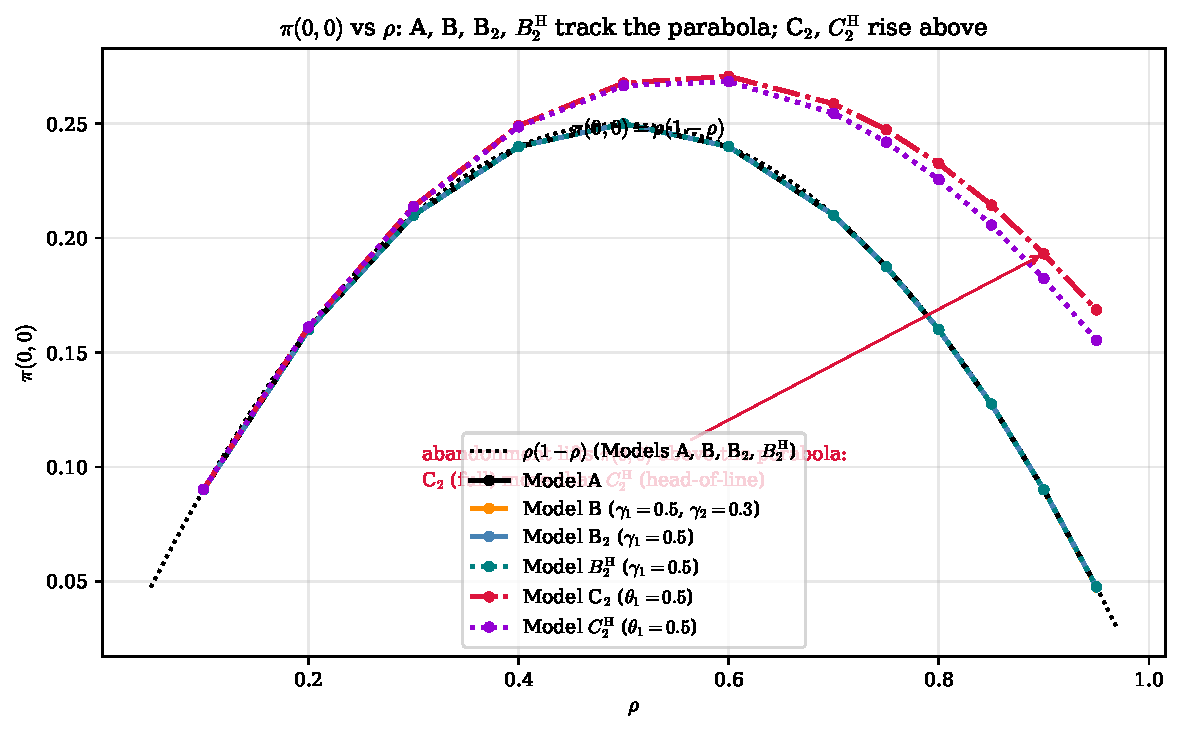
\includegraphics[width=0.78\textwidth]{figures/results/fig_sweep_pi00_vs_rho.pdf}
  \caption{$\pi(0,0)$ versus $\rho$. The three customer-conserving models $A$, $B_2$ and
  $\BH$ lie exactly on the parabola $\rho(1-\rho)$ (Corollaries~\ref{cor:A:pi0},
  \ref{cor:B2:pi00}, \ref{cor:B21:pi0}: jockeying preserves $N$, hence the busy-but-empty
  probability), whereas the abandonment models $C_2$ and $\CH$ rise strictly above it ---
  abandonment inflates $\pi(0,0)$ through the enlarged idle probability $\pi(0,0)=\rho\,\pi_0$
  (Corollaries~\ref{cor:C2:pi00}, \ref{cor:C21:pi0}), the full rate ($C_2$) lifting it more
  than the head-of-line rate ($\CH$).}
  \label{fig:comp:pi00}
\end{figure}
%% END SIMULATION RESULTS — fig_sweep_pi00_vs_rho %%

The invariance of $\pi(0,0)=\rho(1-\rho)$ along the $A$ and $B_2$ curves of
Figure~\ref{fig:comp:pi00} is not a numerical coincidence but a direct reading of
Corollary~\ref{cor:B2:pi00}: the event ``server busy, both queues empty'' depends only on
the total occupancy $N$, and jockeying leaves the law of $N$ unchanged. For $C_2$ the
identity $\pi(0,0)=\rho\,\pi_0$ still holds, but $\pi_0>1-\rho$, so the curve is lifted ---
at $\rho=0.70$, $\pi(0,0)=\piZZCtwoSeventy$ against the baseline $\piZZASeventy$
(Table~\ref{tab:comp:main}). The lift is also asymmetric: whereas the conserving parabola
$\rho(1-\rho)$ is symmetric about $\rho=\tfrac12$, the $C_2$ curve in
Figure~\ref{fig:comp:pi00} attains its maximum to the \emph{right} of that point, the
signature of abandonment renormalising the effective load --- the busy-but-empty probability
keeps climbing past the symmetric-load peak because the self-regulating valve blunts
congestion fastest exactly where the baseline is heaviest, before the shrinking busy fraction
finally pulls it down.

\subsubsection{Companion loss-accounting and queue-length tables}

The class-1 loss accounting that accompanies Table~\ref{tab:comp:main} is collected in
Table~\ref{tab:comp:loss_acct}: in every row the carried throughput and the abandonment
rate sum to the offered load $\rho$, and only the abandonment models $C_2$ and $\CH$ carry a
positive loss fraction $L_1$.

% Companion loss-accounting table. Hand-authored but every number is sourced from
% results/derived_metrics.tex (D1 pipeline); re-run Code/compute_derived_metrics.py to
% regenerate the macros. Kept separate from Table~\ref{tab:comp:main} to stay within margins.
\begin{table}[H]\centering
\caption{Class-1 loss accounting accompanying Table~\ref{tab:comp:main}, at the same three
loads and parameters ($\lambda_1{:}\lambda_2=3{:}4$, $\mu=1$; mechanism parameter $0.5$).
\emph{Throughput} is the carried rate $\mu(1-\pi_0)$; \emph{abandonment rate} is the class-1
loss flow ($\theta_1\mathbb{E}[N_1]$ for the full rate, $\theta_1\mathbb{P}(N_1\ge1)$ for
head-of-line); and $L_1=\theta_1\mathbb{E}[N_1]/\lambda_1$ is the fraction
of class-1 arrivals shed before service (eq.~\eqref{eq:comp:lossfrac}). The conserving models
$A$, $B_2$, $\BH$ lose nothing; only $C_2$ and $\CH$ have $L_1>0$, and at
every row throughput${}+{}$abandonment rate${}={}$offered load $\rho$.}
\label{tab:comp:loss_acct}
\begin{tabular}{llrrr}
\toprule
$\rho$ & Model & Throughput & Aband.\ rate & $L_1$ \\
\midrule
\multirow{5}{*}{0.50} & A & \throughputAFifty & $0$ & $0$ \\
 & B$_2$ & \throughputBtwoFifty & $0$ & $0$ \\
 & $\BH$ & \throughputBHFifty & $0$ & $0$ \\
 & C$_2$ & \throughputCtwoFifty & \lostflowCtwoFifty & \lossCtwoFifty \\
 & $\CH$ & \throughputCHFifty & \lostflowCHFifty & \lossCHFifty \\
\midrule
\multirow{5}{*}{0.70} & A & \throughputASeventy & $0$ & $0$ \\
 & B$_2$ & \throughputBtwoSeventy & $0$ & $0$ \\
 & $\BH$ & \throughputBHSeventy & $0$ & $0$ \\
 & C$_2$ & \throughputCtwoSeventy & \lostflowCtwoSeventy & \lossCtwoSeventy \\
 & $\CH$ & \throughputCHSeventy & \lostflowCHSeventy & \lossCHSeventy \\
\midrule
\multirow{5}{*}{0.90} & A & \throughputANinety & $0$ & $0$ \\
 & B$_2$ & \throughputBtwoNinety & $0$ & $0$ \\
 & $\BH$ & \throughputBHNinety & $0$ & $0$ \\
 & C$_2$ & \throughputCtwoNinety & \lostflowCtwoNinety & \lossCtwoNinety \\
 & $\CH$ & \throughputCHNinety & \lostflowCHNinety & \lossCHNinety \\
\bottomrule
\end{tabular}
\end{table}

%% BEGIN SIMULATION RESULTS — tab_EN_sweep %%
\begin{table}[t]\centering
\caption{Class-1 mean queue length $E[N_1]$ and waiting time $E[W_1]$ under Models A, B$_2$ ($\gamma_1=0.5$) and C$_2$ ($\theta_1=0.5$), with $\mu=1$ and $\lambda_1{:}\lambda_2=3{:}4$.}
\label{tab:comp:EN_sweep}
\begin{tabular}{lrrrrrr}
\toprule
 & \multicolumn{3}{c}{$E[N_1]$} & \multicolumn{3}{c}{$E[W_1]$} \\
\cmidrule(lr){2-4}\cmidrule(lr){5-7}
$\rho$ & A & B$_2$ & C$_2$ & A & B$_2$ & C$_2$ \\
\midrule
0.50 & 0.1364 & 0.0767 & 0.0712 & 0.6364 & 0.3578 & 0.3323 \\
0.70 & 0.3000 & 0.1545 & 0.1392 & 1.0000 & 0.5151 & 0.4639 \\
0.90 & 0.5651 & 0.2626 & 0.2292 & 1.4651 & 0.6808 & 0.5941 \\
\bottomrule
\end{tabular}
\end{table}

%% END SIMULATION RESULTS — tab_EN_sweep %%

Table~\ref{tab:comp:EN_sweep} reads off the per-class queue lengths and waiting times across
the sweep. The priority waiting time $\mathbb{E}[W_1]$ is smallest for $C_2$ at every load
($\EWoneCtwoNinety$ at $\rho=0.90$ against $\EWoneBtwoNinety$ for $B_2$ and $\EWoneANinety$ for $A$), but
$\mathbb{E}[W_i]=\mathbb{E}[N_i]/\lambda_i$ is the mean time a customer is \emph{counted in
queue~$i$}, and that residence is shortened by every departure mode --- service,
\emph{and} attrition. In $C_2$ a class-1 customer leaves the count by being served
\emph{or} by abandoning; in $B_2$ by being served \emph{or} by jockeying into class~2.
A smaller $\mathbb{E}[W_1]$ therefore does not by itself certify faster service, and
cross-model $\mathbb{E}[W_1]$ comparisons conflate latency reduction with customer loss; the
loss fraction $L_1$ of \S\ref{subsec:comp:abandonment} measures exactly the size of that
confound.

\subsubsection{The jockeying mechanism (Model \texorpdfstring{$B_2$}{B2})}
\label{subsec:comp:jockeying}

Figure~\ref{fig:b2:jockeying} isolates the action of $\gamma_1$ at fixed load $\rho=0.70$,
sweeping $\gamma_1\in[10^{-3},50]$.

%% BEGIN SIMULATION RESULTS — fig_B2_jockeying_EN_vs_gamma1 %%
\begin{figure}[H]
  \centering
  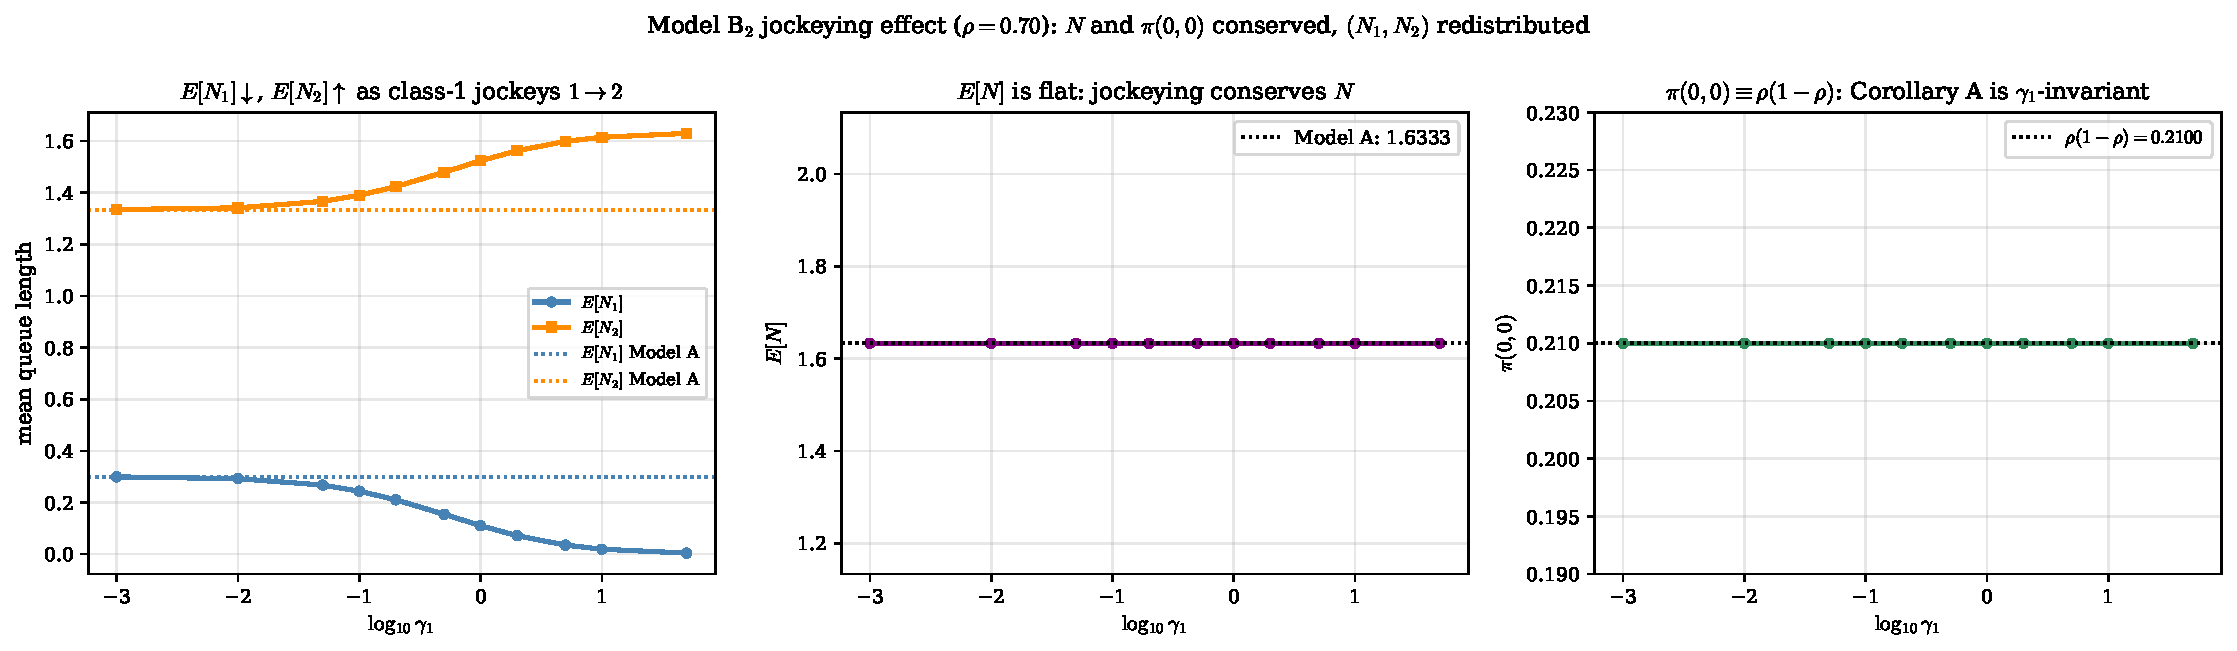
\includegraphics[width=0.98\textwidth]{figures/results/fig_B2_jockeying_EN_vs_gamma1.pdf}
  \caption{Model-$B_2$ at $\rho=0.70$ ($\lambda_1=0.3$, $\lambda_2=0.4$, $\mu=1$).
  \emph{Left:} $\mathbb{E}[N_1]$ decreases and $\mathbb{E}[N_2]$ increases monotonically in
  $\gamma_1$ (Model-$A$ values dotted). \emph{Centre:} $\mathbb{E}[N]$ is flat ---
  jockeying conserves the total count. \emph{Right:} $\pi(0,0)\equiv\rho(1-\rho)=0.21$ for
  all $\gamma_1$, the numerical signature of Corollary~\ref{cor:B2:pi00}.}
  \label{fig:b2:jockeying}
\end{figure}
%% END SIMULATION RESULTS — fig_B2_jockeying_EN_vs_gamma1 %%

The monotone decrease of $\mathbb{E}[N_1]$ in $\gamma_1$ follows directly from the rate
structure: each waiting class-1 customer generates a jockeying event at rate $\gamma_1$, so
the expected outflow from the class-1 queue is $\gamma_1\mathbb{E}[N_1]$, an additional
drain that acts independently of the service process and grows with $\gamma_1$. At
$\gamma_1=0.5$ this halves the priority queue, from $\mathbb{E}[N_1]=\ENoneASeventy$ to $\ENoneBtwoSeventy$
($-\ENoneBtwoReductionSeventy\%$, Table~\ref{tab:comp:main}). The mass is not destroyed but transferred:
$\mathbb{E}[N_2]$ rises correspondingly from $\ENtwoASeventy$ to $\ENtwoBtwoSeventy$, and the centre panel
confirms $\mathbb{E}[N]=\ENASeventy$ is held constant to plotting precision. The right panel is
the cleanest empirical check of Corollary~\ref{cor:B2:pi00}: because every jockeying
transition preserves $N$, the load on the server --- and therefore $\pi_0=1-\rho$ and
$\pi(0,0)=\rho(1-\rho)=0.21$ --- is exactly $\gamma_1$-invariant.

%% BEGIN SIMULATION RESULTS — fig_B2_priority_ratio_vs_gamma1 %%
\begin{figure}[H]
  \centering
  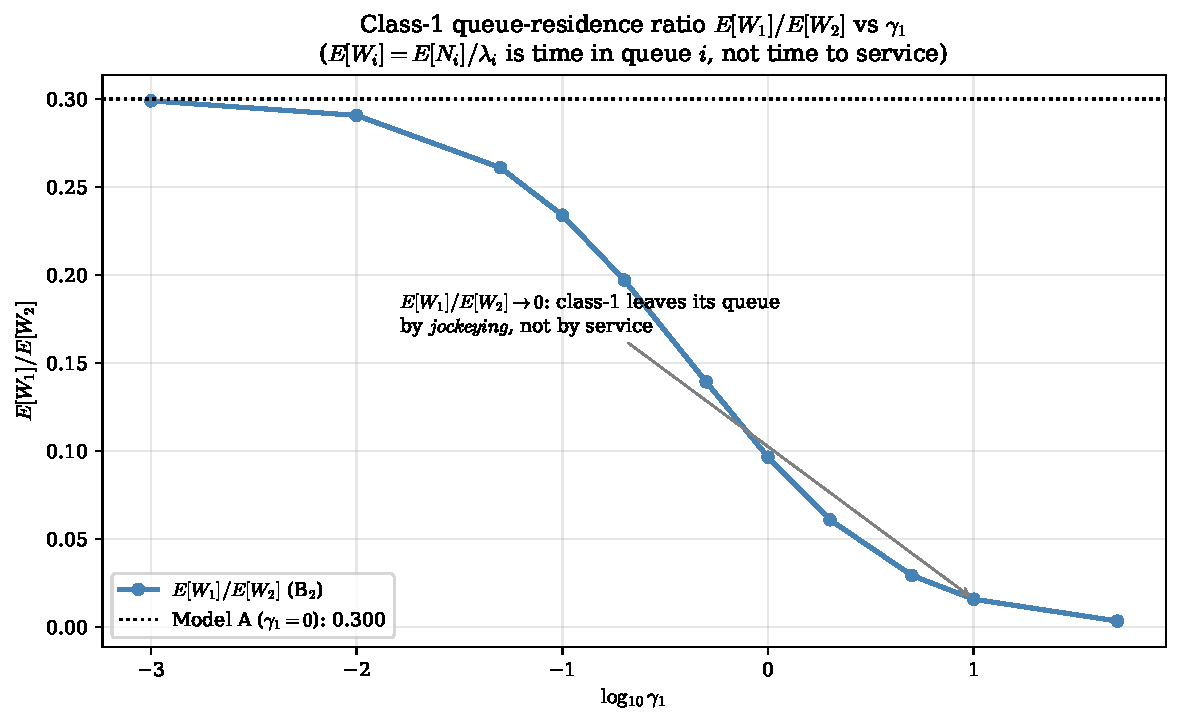
\includegraphics[width=0.80\textwidth]{figures/results/fig_B2_priority_ratio_vs_gamma1.pdf}
  \caption{Class-1 queue-residence ratio $\mathbb{E}[W_1]/\mathbb{E}[W_2]$ versus
  $\gamma_1$ at $\rho=0.70$, with the Model-$A$ value dotted. The ratio decreases toward
  zero because $\mathbb{E}[W_1]=\mathbb{E}[N_1]/\lambda_1$ measures time spent in the
  class-1 queue, which the jockeying drain $\gamma_1\mathbb{E}[N_1]$ collapses; it does not
  measure time to service.}
  \label{fig:b2:priority}
\end{figure}
%% END SIMULATION RESULTS — fig_B2_priority_ratio_vs_gamma1 %%

Figure~\ref{fig:b2:priority} must be read with the residence-time caveat of
\S\ref{subsec:comp:sweep} firmly in mind. As $\gamma_1$ grows the ratio
$\mathbb{E}[W_1]/\mathbb{E}[W_2]$ falls monotonically from the Model-$A$ value of $0.300$
toward zero, which would naively suggest an ever-improving class-1 service. The mechanism
is the opposite: a large $\gamma_1$ ejects class-1 customers from their own queue almost
immediately, so the \emph{count} $\mathbb{E}[N_1]$ and hence $\mathbb{E}[W_1]$ vanish, but
the ejected customers simply wait out their delay at the back of the class-2 queue. The
falling ratio records the dissolution of the class-1 queue, not an acceleration of class-1
service. This is the precise sense in which strong one-way jockeying \emph{erodes the
priority structure}: in the limit there is effectively a single class.

\subsubsection{Class asymmetry}
\label{subsec:comp:asymmetry}

Fixing $\rho=0.70$ and varying the split $\alpha=\lambda_1/(\lambda_1+\lambda_2)$ exposes
how the mechanisms interact with the class mix. Figure~\ref{fig:comp:asymmetry} compares the
three models; Figure~\ref{fig:b2:asymmetry} resolves the jockeying case at three rates.

%% BEGIN SIMULATION RESULTS — fig_class_asymmetry %%
\begin{figure}[H]
  \centering
  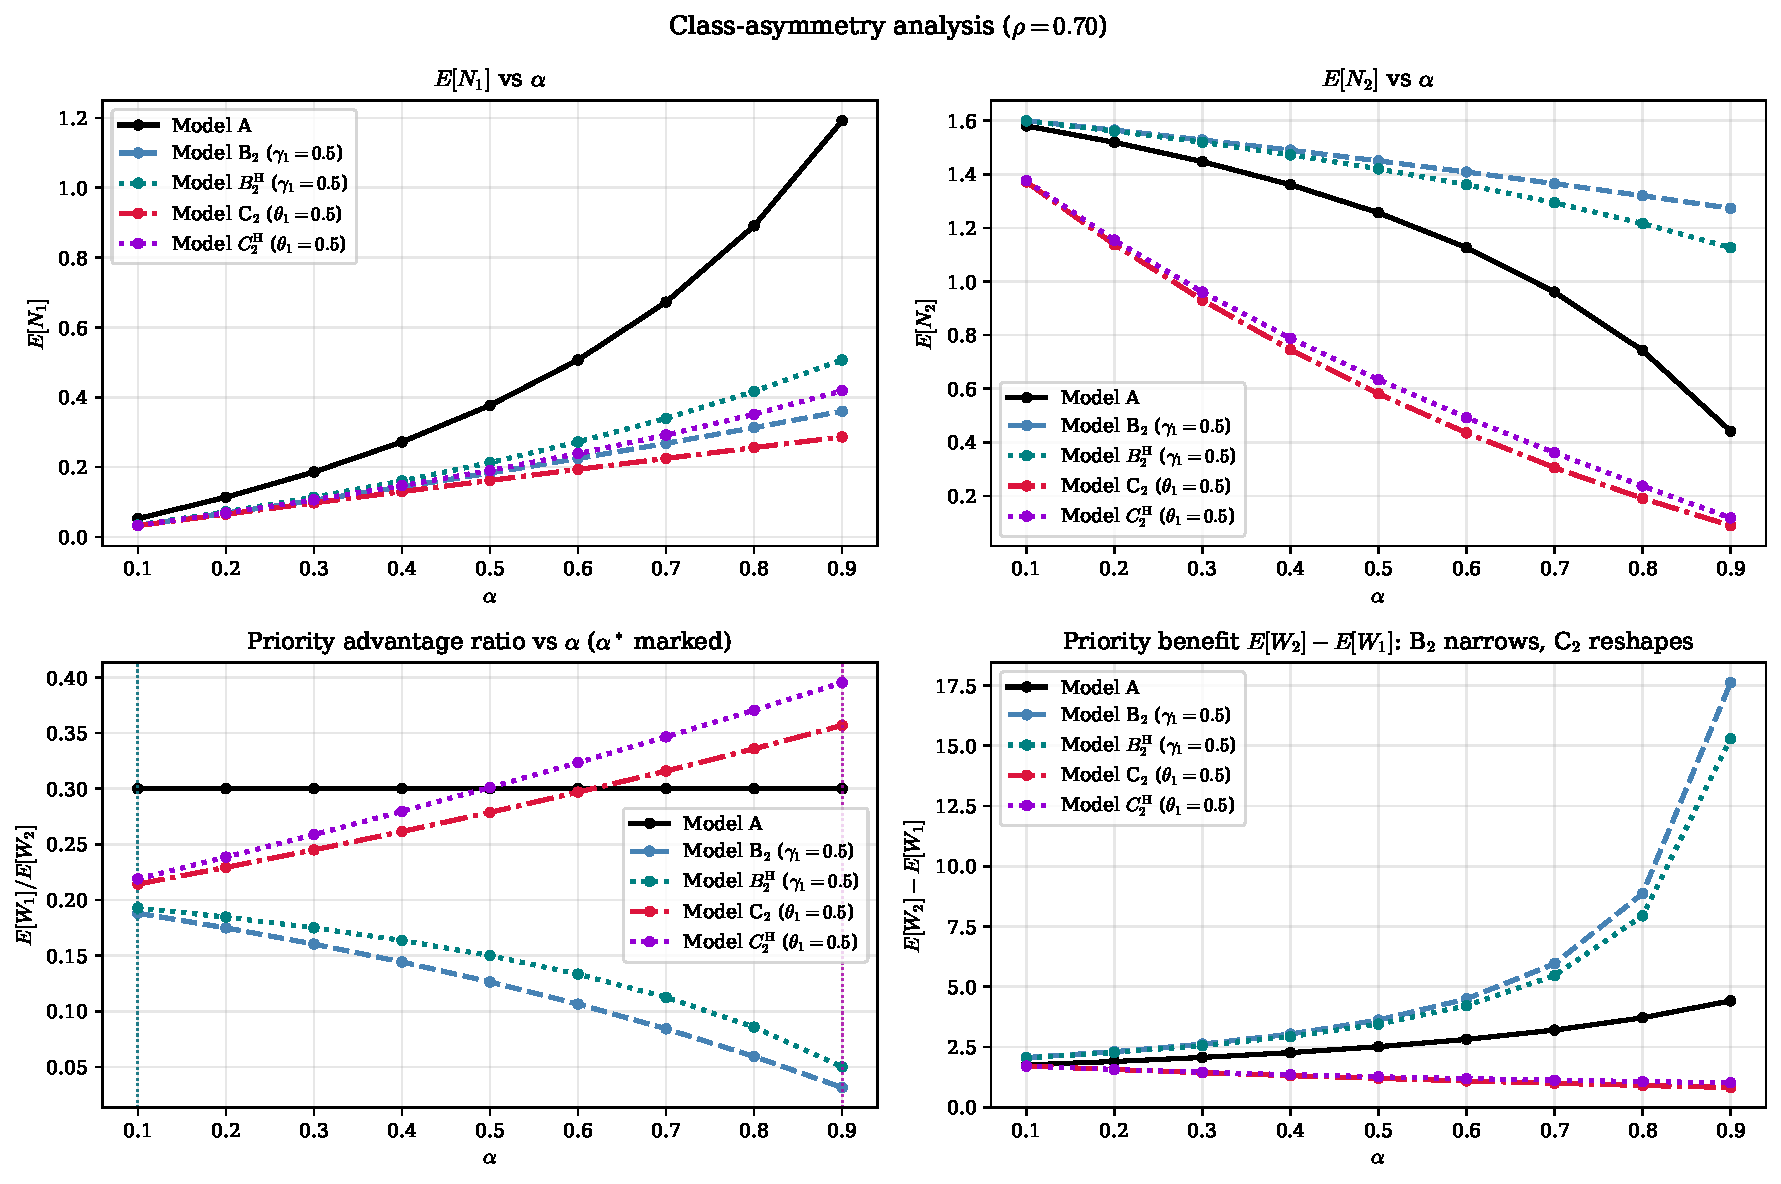
\includegraphics[width=0.98\textwidth]{figures/results/fig_class_asymmetry.pdf}
  \caption{Class-asymmetry sweep at $\rho=0.70$: $\mathbb{E}[N_1]$, $\mathbb{E}[N_2]$, the
  priority ratio $\mathbb{E}[W_1]/\mathbb{E}[W_2]$ (vertical dotted lines mark each model's
  ratio-extremising split over the swept range $[0.1,0.9]$), and the absolute priority
  benefit $\mathbb{E}[W_2]-\mathbb{E}[W_1]$, for Models $A$, $B_2$ and $\BH$
  ($\gamma_1=0.5$), and $C_2$ and $\CH$ ($\theta_1=0.5$).}
  \label{fig:comp:asymmetry}
\end{figure}
%% END SIMULATION RESULTS — fig_class_asymmetry %%

As $\alpha\to0$ the priority class is vanishingly rare and its mechanism barely engages:
all models converge in $\mathbb{E}[N_1]$. As $\alpha\to1$ the priority class
dominates the offered load and the non-preemptive discipline gives it near-exclusive access
to the server, driving $\mathbb{E}[N_1]\to0$ in every model. The interesting behaviour is
interior. The absolute priority benefit $\mathbb{E}[W_2]-\mathbb{E}[W_1]$ (bottom-right) is
largest where class~2 bears the most displaced load; jockeying narrows this gap relative to
$A$ by exporting class-1 delay into the class-2 statistic, while abandonment reshapes it by
removing class-1 work outright.

The priority ratio $\mathbb{E}[W_1]/\mathbb{E}[W_2]$ (bottom-left) carries the sharpest
structural signal. For Model-$A$ it is \emph{exactly $\alpha$-invariant}: writing the ratio
as $\mathbb{E}[W_1]/\mathbb{E}[W_2]=(\mathbb{E}[N_1]\,\lambda_2)/(\mathbb{E}[N_2]\,\lambda_1)$
and substituting the closed forms $\mathbb{E}[N_1]=\rho\rho_1/(1-\rho_1)$ and
$\mathbb{E}[N]=\rho^2/(1-\rho)$ collapses the split dependence entirely,
\begin{equation*}
  \left.\frac{\mathbb{E}[W_1]}{\mathbb{E}[W_2]}\right|_{A}=1-\rho
  \qquad\text{for every }\alpha\in(0,1),
\end{equation*}
the flat line at $\ratioPeakA=1-\rho$ in the panel. The two mechanisms break this invariance
in \emph{opposite, monotone} directions. Jockeying makes the ratio strictly \emph{decreasing}
in $\alpha$, so it peaks at $\ratioPeakBtwo$ at the left endpoint $\alpha^\ast=\alphaStarBtwo$
(a larger priority share feeds the $1\!\to\!2$ drain harder); abandonment makes it strictly
\emph{increasing}, peaking at $\ratioPeakCtwo$ at the right endpoint
$\alpha^\ast=\alphaStarCtwo$ (a larger priority share is exactly where the abandonment valve
sheds the most class-1 work). The head-of-line variants track their parents --- $\BH$ peaks at
$\ratioPeakBH$ ($\alpha^\ast=\alphaStarBH$) and $\CH$ at $\ratioPeakCH$
($\alpha^\ast=\alphaStarCH$) --- and are likewise monotone. No curve turns over: across all
five models the maximiser $\alpha^\ast$ sits at a \emph{boundary} of the swept range
$[0.1,0.9]$, never at an interior point. An interior $\alpha^\ast$ would require mechanism
engagement (which strengthens as the priority class grows) to balance class dominance at some
intermediate split; here the two effects pull the ratio the same way throughout, so the
extremum is always pushed to an endpoint.

%% BEGIN SIMULATION RESULTS — fig_B2_class_asymmetry_gamma1 %%
\begin{figure}[H]
  \centering
  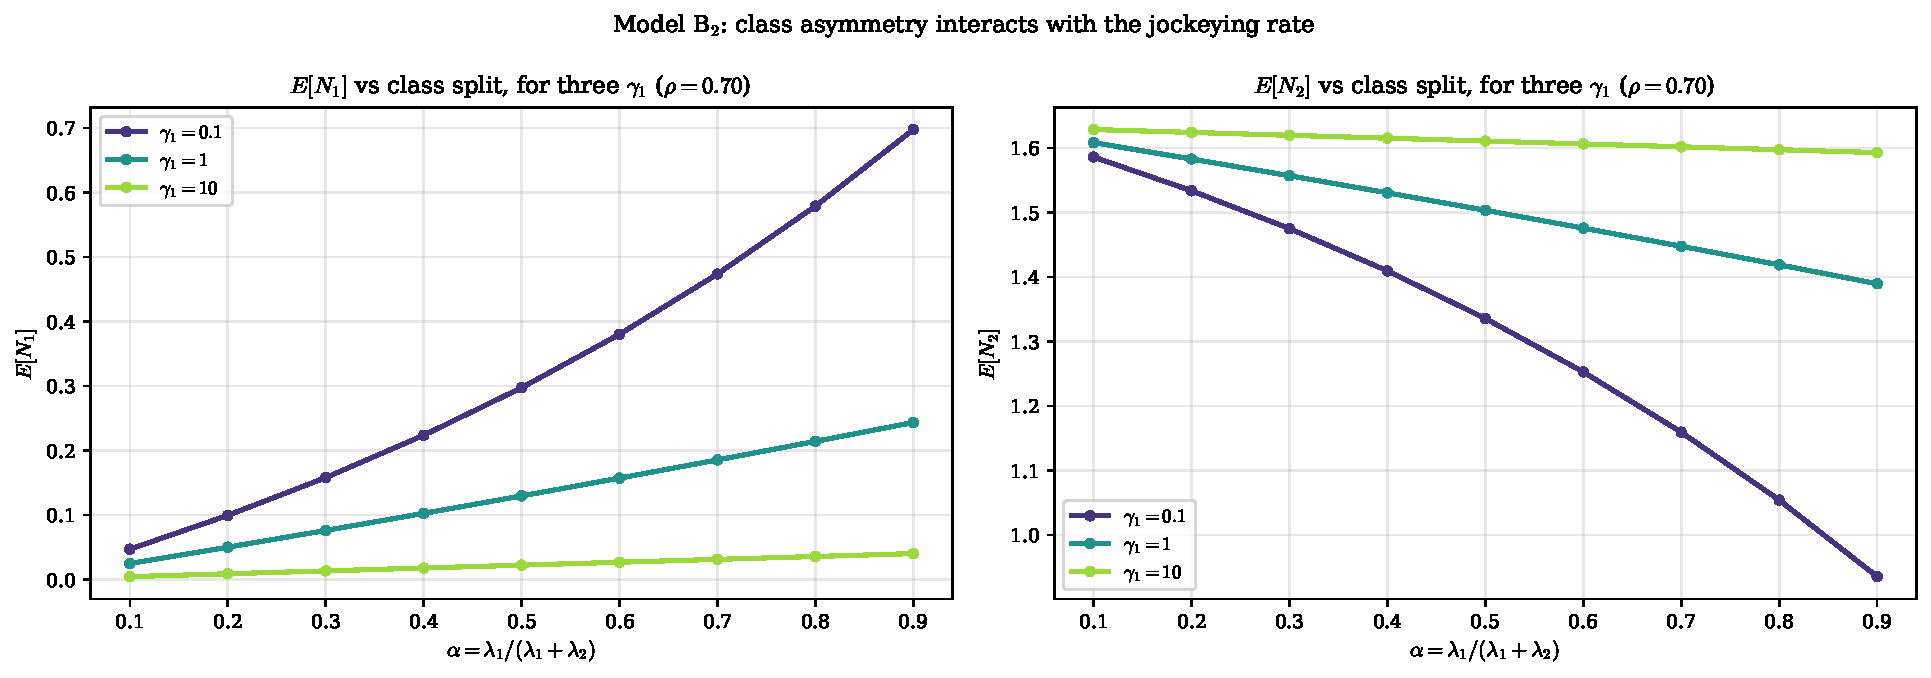
\includegraphics[width=0.98\textwidth]{figures/results/fig_B2_class_asymmetry_gamma1.pdf}
  \caption{Model-$B_2$: $\mathbb{E}[N_1]$ and $\mathbb{E}[N_2]$ versus the split $\alpha$
  for three jockeying rates $\gamma_1\in\{0.1,1.0,10.0\}$ at $\rho=0.70$. Stronger
  jockeying flattens $\mathbb{E}[N_1]$ toward zero across the whole range of $\alpha$ and
  loads the difference onto $\mathbb{E}[N_2]$.}
  \label{fig:b2:asymmetry}
\end{figure}
%% END SIMULATION RESULTS — fig_B2_class_asymmetry_gamma1 %%

The family in Figure~\ref{fig:b2:asymmetry} shows that the jockeying drain dominates the
class mix: at $\gamma_1=10$ the priority queue is essentially empty for every $\alpha$,
because the per-customer ejection rate $\gamma_1$ overwhelms the arrival rate $\lambda_1$
regardless of the split. At $\gamma_1=0.1$ the curves still track the Model-$A$ shape, the
drain being a small perturbation. The crossover between these regimes occurs where
$\gamma_1$ is comparable to the effective class-1 service rate, consistent with the
singular role of $\gamma_1$ in the $B_2$ ODE.

\subsubsection{The abandonment mechanism (Model \texorpdfstring{$C_2$}{C2})}

Figure~\ref{fig:c2:abandonment} sweeps $\theta_1\in[10^{-3},50]$ at $\rho=0.70$.

%% BEGIN SIMULATION RESULTS — fig_C2_abandonment_EN_vs_theta1 %%
\begin{figure}[H]
  \centering
  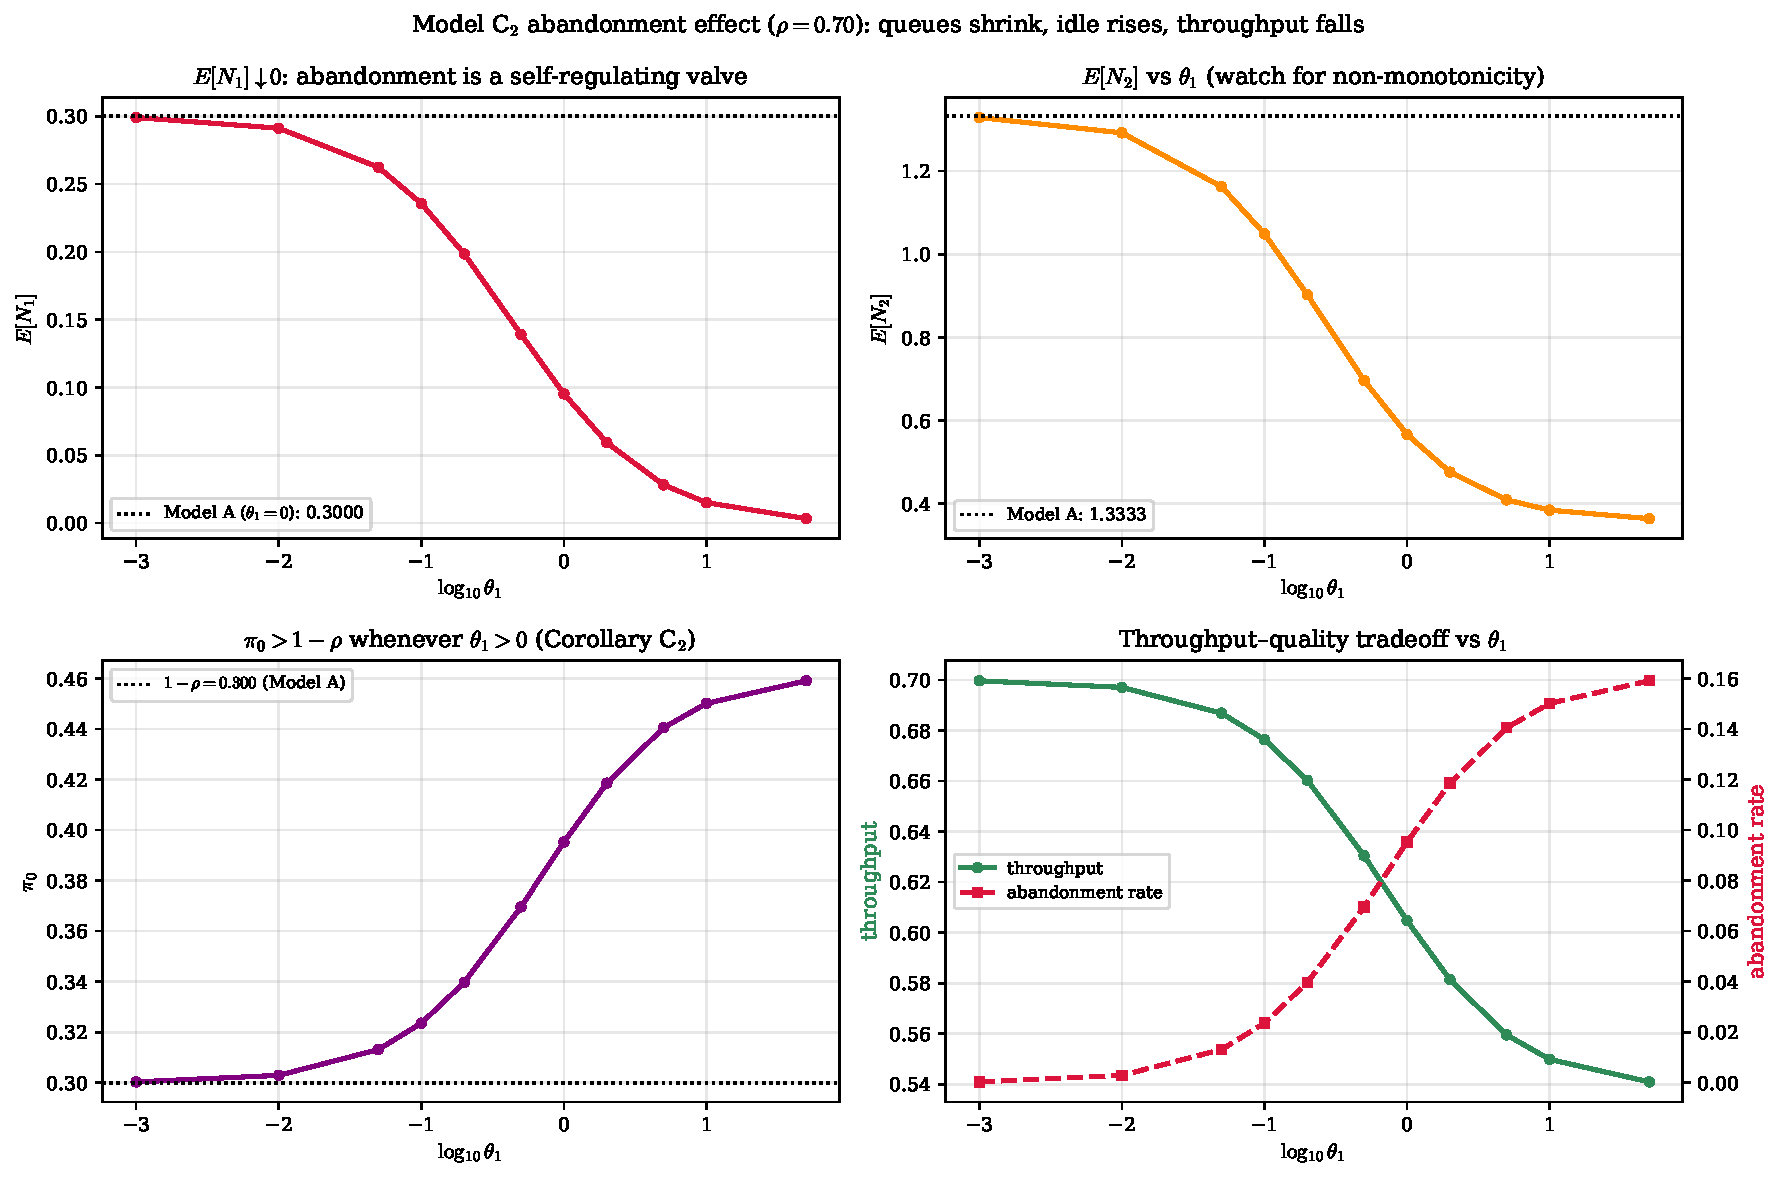
\includegraphics[width=0.98\textwidth]{figures/results/fig_C2_abandonment_EN_vs_theta1.pdf}
  \caption{Model-$C_2$ at $\rho=0.70$. \emph{Top-left:} $\mathbb{E}[N_1]\to0$ as the
  abandonment valve $\theta_1 n_1$ strengthens. \emph{Top-right:} $\mathbb{E}[N_2]$
  \emph{decreases monotonically} (no rebound at these parameters). \emph{Bottom-left:}
  $\pi_0>1-\rho$ for all $\theta_1>0$ (Corollary~\ref{cor:C2:pi00}). \emph{Bottom-right:}
  the throughput--quality tradeoff --- throughput falls and the abandonment rate rises with
  $\theta_1$.}
  \label{fig:c2:abandonment}
\end{figure}
%% END SIMULATION RESULTS — fig_C2_abandonment_EN_vs_theta1 %%

The priority queue $\mathbb{E}[N_1]$ collapses toward zero as $\theta_1$ grows: the
abandonment outflow $\theta_1\mathbb{E}[N_1]$ is a self-regulating valve that opens wider
the longer the queue, so no class-1 backlog can persist. The idle-probability panel is the
empirical face of Corollary~\ref{cor:C2:pi00}: every positive $\theta_1$ lifts $\pi_0$
strictly above the Model-$A$ value $1-\rho=0.30$, because customers who abandon never reach
the server and the busy fraction shrinks accordingly. This sweep also settles, as a
\emph{negative finding}, a question flagged in the simulation
brief. Two effects compete in $\mathbb{E}[N_2]$ as $\theta_1$ rises: abandonment is
class-1-specific, so clearing the priority backlog lets the server reach class~2 sooner --- an
effect that could in principle make $\mathbb{E}[N_2]$ rise transiently before falling --- set
against the plain reduction in the total work the class-2 queue inherits once class~1 is bled
off faster. At $\rho=0.70$ the second effect dominates throughout: $\mathbb{E}[N_2]$ is
\emph{monotonically decreasing} in $\theta_1$ with no initial hump, contradicting the
conjectured non-monotonicity. We observed no rebound at any load tested and conjecture that
$\mathbb{E}[N_2]$ is monotone decreasing in $\theta_1$ for every $\rho<1$; a proof, or a
counterexample at extreme class asymmetry, is left to future work (\S\ref{sec:future_work}).
The bottom-right panel quantifies the price and, in doing so, supplies an independent
numerical check. Throughput falls from the Model-$A$ value $\mu\rho=\offeredSeventy$ to
$\throughputCtwoSeventy$ at $\theta_1=0.5$, a deficit of $\lostflowCtwoSeventy$; computed
\emph{separately} as the abandonment flow $\theta_1\mathbb{E}[N_1]$, the lost rate reproduces
that same $\lostflowCtwoSeventy$, so carried plus lost returns the offered $\offeredSeventy$.
Because the throughput deficit $\mu\rho-\mu(1-\pi_0)$ and the abandonment integral
$\theta_1\mathbb{E}[N_1]$ are distinct functionals of the stationary law --- one read from the
idle probability of Corollary~\ref{cor:C2:pi00}, the other from the mean queue length --- their
agreement is not a restatement of flow balance but an independent verification of both.

%% BEGIN SIMULATION RESULTS — fig_C2_E_BC_vs_theta1 %%
\begin{figure}[H]
  \centering
  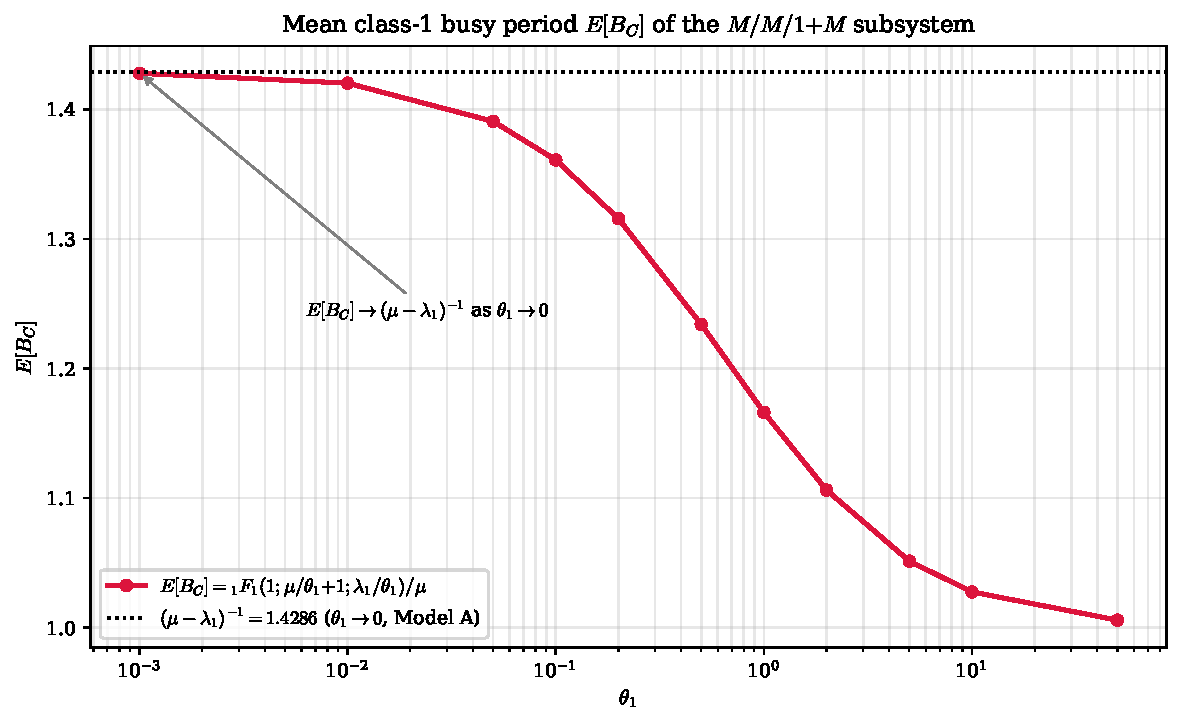
\includegraphics[width=0.78\textwidth]{figures/results/fig_C2_E_BC_vs_theta1.pdf}
  \caption{Mean class-1 busy period $\mathbb{E}[B_C]$ of the $M/M/1{+}M$ subsystem versus
  $\theta_1$, computed in closed form from
  $\mathbb{E}[B_C]={}_1F_1(1;\mu/\theta_1+1;\lambda_1/\theta_1)/\mu$
  (cf.\ \eqref{eq:comp:1F1}). The horizontal asymptote is the Model-$A$ busy period
  $(\mu-\lambda_1)^{-1}=1.4286$, attained as $\theta_1\to0^+$ (Corollary~\ref{cor:C2:pi00}
  limit).}
  \label{fig:c2:ebc}
\end{figure}
%% END SIMULATION RESULTS — fig_C2_E_BC_vs_theta1 %%

The busy-period curve in Figure~\ref{fig:c2:ebc} is the engine of the $C_2$ corollary: the
confluent hypergeometric ${}_1F_1(1;\mu/\theta_1+1;\lambda_1/\theta_1)$ of
\eqref{eq:comp:1F1} interpolates between the abandonment-free busy period and the
fast-clearance regime. As $\theta_1\to0^+$ the Kummer function tends to unity in the
relevant ratio and $\mathbb{E}[B_C]\to(\mu-\lambda_1)^{-1}=1.4286$, recovering the Model-$A$
class-1 busy period; as $\theta_1$ grows the busy period shortens because the server is
relieved by abandonment as well as by service.

\subsubsection{The priority benefit}

%% BEGIN SIMULATION RESULTS — tab_priority_benefit %%
\begin{table}[t]\centering
\caption{Class-1 mean waiting time $E[W_1]$ and priority ratio $E[W_2]/E[W_1]$ under each model ($\lambda_1{:}\lambda_2=3{:}4$, $\mu=1$, $\gamma_1=\theta_1=0.5$).}
\label{tab:prio:benefit}
\begin{tabular}{lrrrrrr}
\toprule
 & \multicolumn{2}{c}{Model A} & \multicolumn{2}{c}{Model B$_2$} & \multicolumn{2}{c}{Model C$_2$} \\
\cmidrule(lr){2-3}\cmidrule(lr){4-5}\cmidrule(lr){6-7}
$\rho$ & $E[W_1]$ & $E[W_2]/E[W_1]$ & $E[W_1]$ & $E[W_2]/E[W_1]$ & $E[W_1]$ & $E[W_2]/E[W_1]$ \\
\midrule
0.50 & 0.6364 & 2.0000 & 0.3578 & 4.1411 & 0.3323 & 2.6551 \\
0.70 & 1.0000 & 3.3333 & 0.5151 & 7.1774 & 0.4639 & 3.7545 \\
0.90 & 1.4651 & 9.9996 & 0.6808 & 22.3834 & 0.5941 & 6.2985 \\
\bottomrule
\end{tabular}
\end{table}

%% END SIMULATION RESULTS — tab_priority_benefit %%

Table~\ref{tab:prio:benefit} contrasts the priority structure directly. The ratio
$\mathbb{E}[W_2]/\mathbb{E}[W_1]$ measures how strongly the discipline favours class~1.
Jockeying inflates this ratio sharply --- to $\premiumBtwoSeventy$ at $\rho=0.70$ and
$\premiumBtwoNinety$ at $\rho=0.90$, against the baseline $\premiumASeventy$ and
$\premiumANinety$ --- but, as established in \S\ref{sec:comparison}, the inflation reflects the
collapse of the class-1 \emph{queue} (its residence time, not its service time) and a
simultaneous lengthening of class~2. Abandonment moves the ratio in the opposite direction at
high load ($\premiumCtwoNinety$ at $\rho=0.90$, below the baseline $\premiumANinety$), because
it compresses both waiting times by shedding load. The two mechanisms are thus not
substitutes: jockeying redistributes delay between classes at fixed total work, whereas
abandonment reduces total work at the cost of served throughput.

The $\rho=0.90$ row of Table~\ref{tab:prio:benefit} is the single sharpest statement of this
dichotomy. Under one and the same non-preemptive discipline the priority premium
$\mathbb{E}[W_2]/\mathbb{E}[W_1]$ moves to $\premiumBtwoNinety$ under jockeying and to
$\premiumCtwoNinety$ under abandonment, straddling the Model-$A$ baseline of $\premiumANinety$
in \emph{opposite} directions. Both models look ``better for class~1'' on the raw
$\mathbb{E}[W_1]$ column, yet for incompatible reasons --- jockeying widens the premium by
exporting class-1 delay onto class~2 at conserved total work, abandonment narrows it by
deleting class-1 work outright. Neither improvement is the naive one, faster service: reading
the premium without the loss fraction of \S\ref{subsec:comp:abandonment} would mistake
redistribution and attrition for speed.

\subsubsection{Head-of-line versus full-rate mechanisms (Models \texorpdfstring{$\BH$}{B2-H} and \texorpdfstring{$\CH$}{C2-H})}
\label{subsec:comp:hol}

The head-of-line models of \S\ref{sec:model_b21}--\ref{sec:model_c21} replace the
\emph{length-proportional} mechanism rate of $B_2$ and $C_2$ --- $\gamma_1 n_1$ or
$\theta_1 n_1$, in which every waiting class-1 customer participates --- by a
\emph{head-of-line} rate $\gamma_1\mathbf 1_{\{n_1\ge1\}}$ or $\theta_1\mathbf 1_{\{n_1\ge1\}}$,
in which only the customer at the head of Queue~1 may jockey or abandon. The aggregate
class-1 outflow is therefore capped at the single rate $\gamma_1$ (or $\theta_1$) instead of
growing with the queue, so each head-of-line mechanism is a strictly \emph{weaker} drain of
the priority queue than its full-rate counterpart. Figure~\ref{fig:comp:hol} quantifies the
gap at fixed load $\rho=0.70$.

%% BEGIN SIMULATION RESULTS — fig_hol_vs_full %%
\begin{figure}[H]
  \centering
  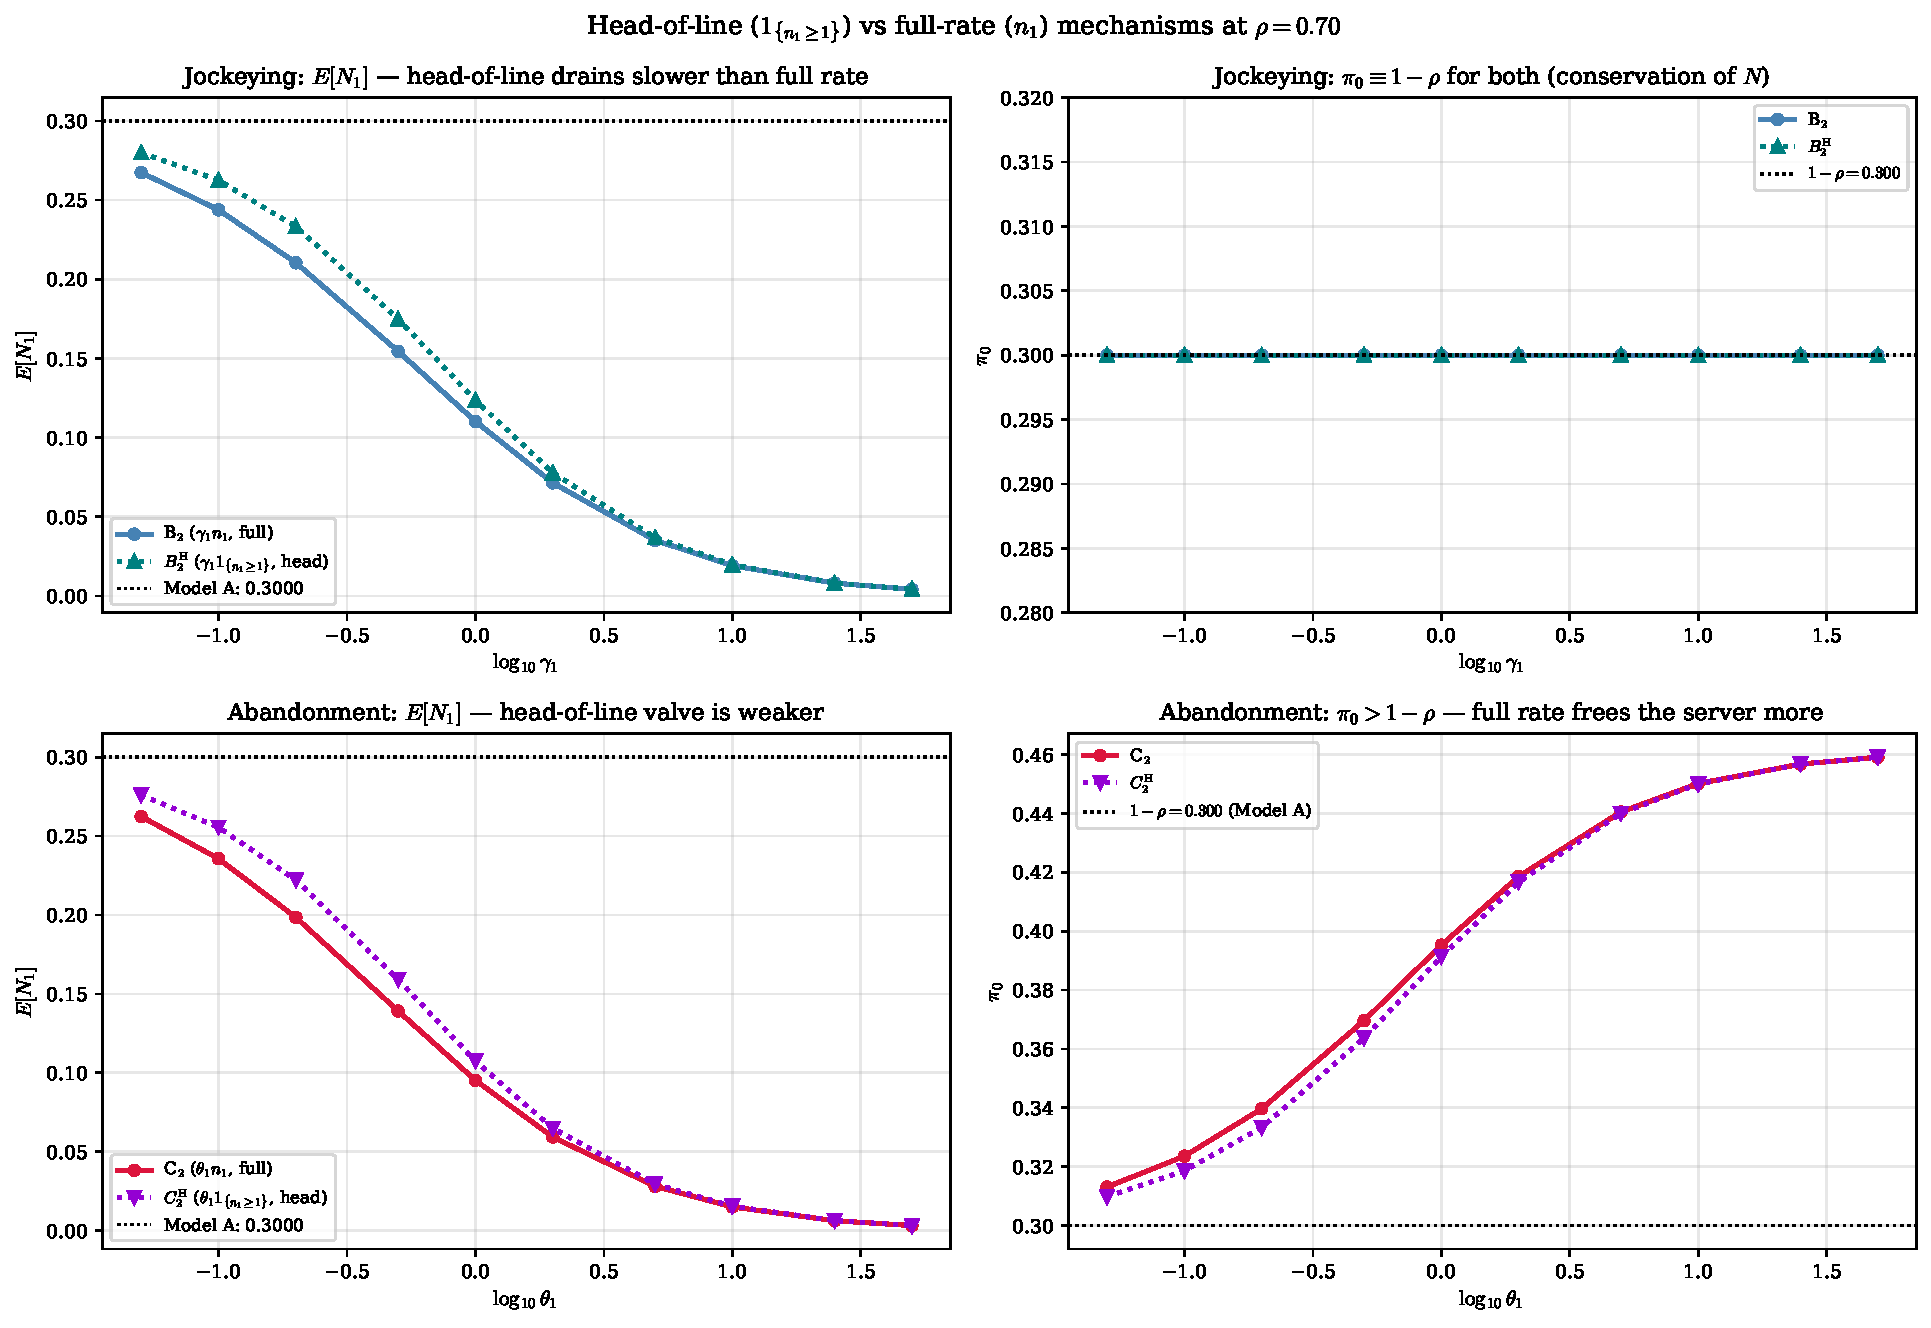
\includegraphics[width=0.98\textwidth]{figures/results/fig_hol_vs_full.pdf}
  \caption{Head-of-line ($\mathbf 1_{\{n_1\ge1\}}$) versus full-rate ($n_1$) mechanisms at
  $\rho=0.70$ ($\lambda_1=0.3$, $\lambda_2=0.4$, $\mu=1$). \emph{Top row, jockeying:}
  $\mathbb{E}[N_1]$ and $\pi_0$ for $B_2$ (full) versus $\BH$ (head-of-line). The
  head-of-line rate drains the priority queue more slowly, so $\mathbb{E}[N_1]$ stays above
  the $B_2$ curve, while $\pi_0\equiv1-\rho$ for both (jockeying conserves $N$,
  Corollaries~\ref{cor:B2:pi00}, \ref{cor:B21:pi0}). \emph{Bottom row, abandonment:}
  $\mathbb{E}[N_1]$ and $\pi_0$ for $C_2$ (full) versus $\CH$ (head-of-line). The
  head-of-line valve is weaker, so $\CH$ retains a slightly longer priority queue and a
  slightly smaller idle gain than $C_2$, both models exceeding the $1-\rho$ baseline
  (Corollaries~\ref{cor:C2:pi00}, \ref{cor:C21:pi0}).}
  \label{fig:comp:hol}
\end{figure}
%% END SIMULATION RESULTS — fig_hol_vs_full %%

The contrast is governed by the number of \emph{waiting} class-1 customers. When the
priority queue holds $n_1\ge2$, the full rate ejects customers at $n_1\gamma_1$ (or
$n_1\theta_1$), a factor of $n_1$ faster than the head-of-line rate $\gamma_1$ (or
$\theta_1$); when $n_1\le1$ the two rates coincide. The head-of-line model is therefore the
weaker drain precisely to the extent that $\mathbb{P}(N_1\ge2)$ carries mass, which is
greatest at intermediate mechanism rates and vanishes both as the rate $\to0$ (the queue is
rarely occupied beyond the head) and as the rate $\to\infty$ (the queue is emptied). The top
panels of Figure~\ref{fig:comp:hol} show this directly: at $\gamma_1=0.5$ the full rate cuts
$\mathbb{E}[N_1]$ from the Model-$A$ value $\ENoneASeventy$ to $\ENoneBtwoSeventy$ ($-\ENoneBtwoReductionSeventy\%$), whereas the
head-of-line rate reaches only $\ENoneBHSeventy$ ($-\ENoneBHReductionSeventy\%$); by $\gamma_1=50$ both have collapsed to
$\mathbb{E}[N_1]\approx0.004$ and the curves are indistinguishable.

This proxy can be read off the numbers directly. The full-versus-head-of-line gap in
$\mathbb{E}[N_1]$ grows with load --- $\gapENoneFifty$, $\gapENoneSeventy$, $\gapENoneNinety$
at $\rho=0.50,0.70,0.90$ --- and tracks the second-tail mass $\mathbb{P}(N_1\ge2)$, which over
the same loads is $\PNGetwoBtwoFifty$, $\PNGetwoBtwoSeventy$, $\PNGetwoBtwoNinety$ (Model-$B_2$).
The two move together because the full and head-of-line rates differ only on states with
$n_1\ge2$: where the priority queue seldom holds two or more waiting customers the cap costs
almost nothing, and where it often does the gap widens. The head-of-line $\mathbb{E}[N_1]$
excess is therefore an operational proxy for $\mathbb{P}(N_1\ge2)$, both vanishing at low load
and growing into the congested regime.

Because jockeying conserves the total customer count under either rate
(Corollary~\ref{cor:B21:pi0}), the milder class-1 drain of $\BH$ is mirrored by a milder
class-2 inflation: at $\rho=0.70$, $\mathbb{E}[N_2]=\ENtwoBHSeventy$ for $\BH$ against $\ENtwoBtwoSeventy$ for
$B_2$, and the priority ratio $\mathbb{E}[W_2]/\mathbb{E}[W_1]$ is $\premiumBHSeventy$ for $\BH$ versus
$\premiumBtwoSeventy$ for $B_2$ (Table~\ref{tab:comp:main}). Head-of-line jockeying thus erodes the
priority structure less aggressively than the full mechanism. The abandonment pair tells the
same story on the throughput--quality axis: at $\rho=0.70$ the full rate $C_2$ lifts $\pi_0$
to $\piZeroCtwoSeventy$ and compresses $\mathbb{E}[N]$ to $\ENCtwoSeventy$, while the head-of-line $\CH$ stops
at $\pi_0=\piZeroCHSeventy$ and $\mathbb{E}[N]=\ENCHSeventy$ --- it sheds less load, frees the server less,
and consequently leaves the priority ratio almost unchanged from the baseline
($\mathbb{E}[W_2]/\mathbb{E}[W_1]=\premiumCHSeventy$ for $\CH$ against $\premiumASeventy$ for $A$ and $\premiumCtwoSeventy$ for
$C_2$). In every descriptor the head-of-line variant interpolates monotonically between
Model-$A$ and its full-rate parent, confirming that restricting a mechanism to the head of
the queue yields a genuine but attenuated version of the same effect.

% =====================================================================
\subsection{Convergence to Model \texorpdfstring{$A$}{A}}
\label{app:numerics:convergence}

Every specialised model must recover Model-$A$ as its distinguishing parameter is switched
off. \S\ref{sec:comparison} established this algebraically and Section~\ref{sec:results}
reports the headline first-order rates; here the convergence is characterised figure by
figure, since the \emph{rate} of convergence measures how rapidly a mechanism departs from
the baseline as it is introduced. Convergence is measured in the $L_1$ distance
$\lVert\pi-\pi_A\rVert_1$ between the full joint distributions, supplemented by the
individual descriptors $\pi_0$, $\pi(0,0)$ and $\mathbb{E}[N_1]$.

\subsubsection{Model \texorpdfstring{$C_2$}{C2} as \texorpdfstring{$\theta_1\to0^+$}{theta1 to 0}}

%% BEGIN SIMULATION RESULTS — fig_conv_C2_to_A_L1 %%
\begin{figure}[H]
  \centering
  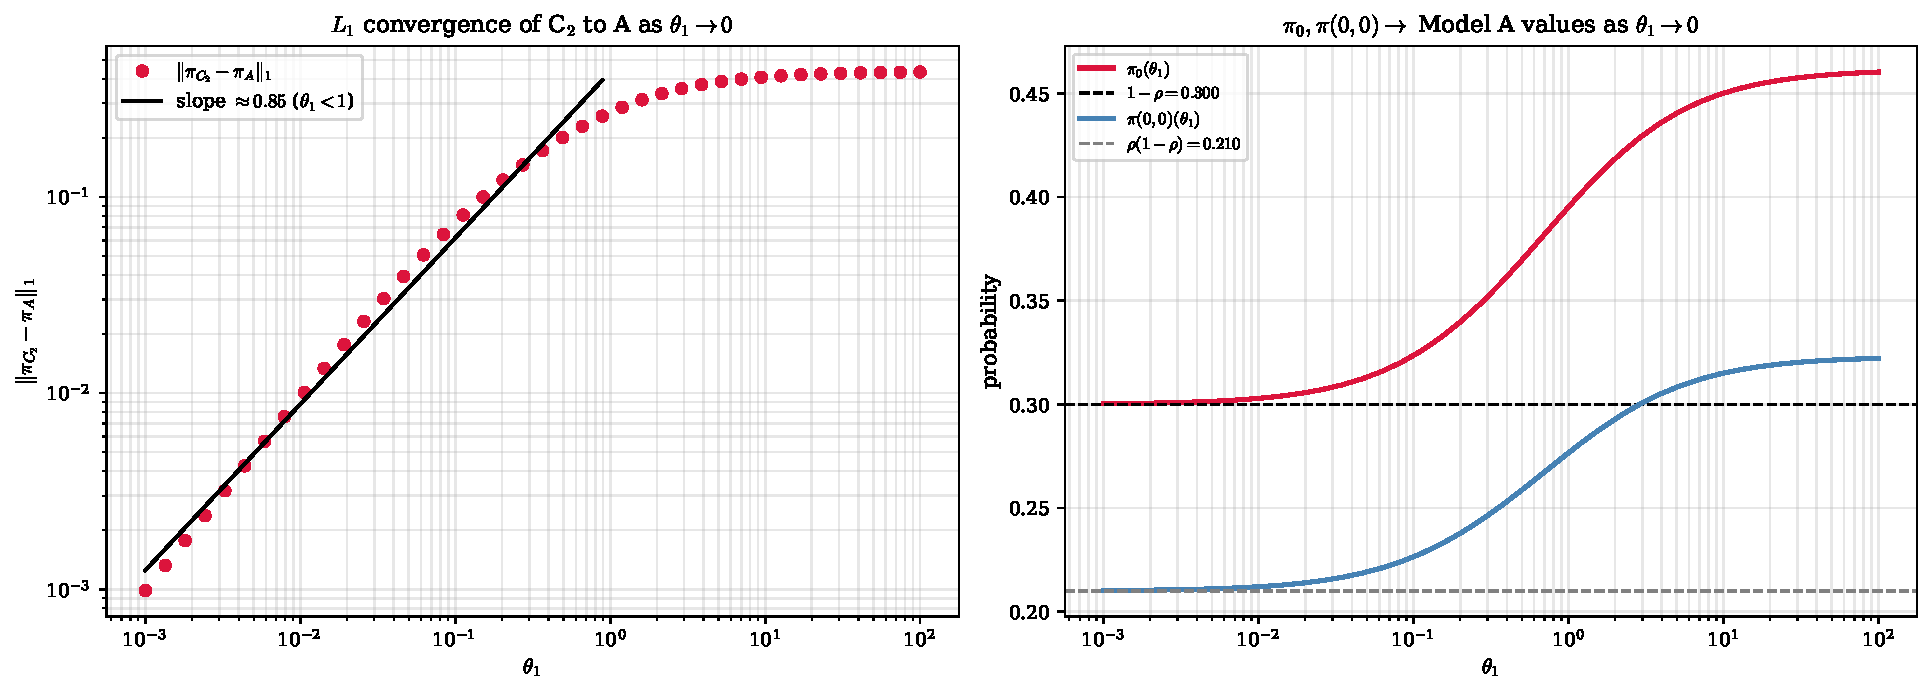
\includegraphics[width=0.98\textwidth]{figures/results/fig_conv_C2_to_A_L1.pdf}
  \caption{Convergence of Model-$C_2$ to Model-$A$ as $\theta_1\to0^+$
  ($\lambda_1=0.3$, $\lambda_2=0.4$, $\mu=1$). \emph{Left:} log--log plot of
  $\lVert\pi_{C_2}-\pi_A\rVert_1$ against $\theta_1$, with a fitted slope of $0.85$ over
  $\theta_1<1$. \emph{Right:} $\pi_0(\theta_1)$ and $\pi(0,0)(\theta_1)$ relaxing onto the
  Model-$A$ values $1-\rho=0.30$ and $\rho(1-\rho)=0.21$ as $\theta_1\to0$.}
  \label{fig:conv:c2_l1}
\end{figure}
%% END SIMULATION RESULTS — fig_conv_C2_to_A_L1 %%

%% BEGIN SIMULATION RESULTS — fig_conv_C2_to_A_indiv %%
\begin{figure}[H]
  \centering
  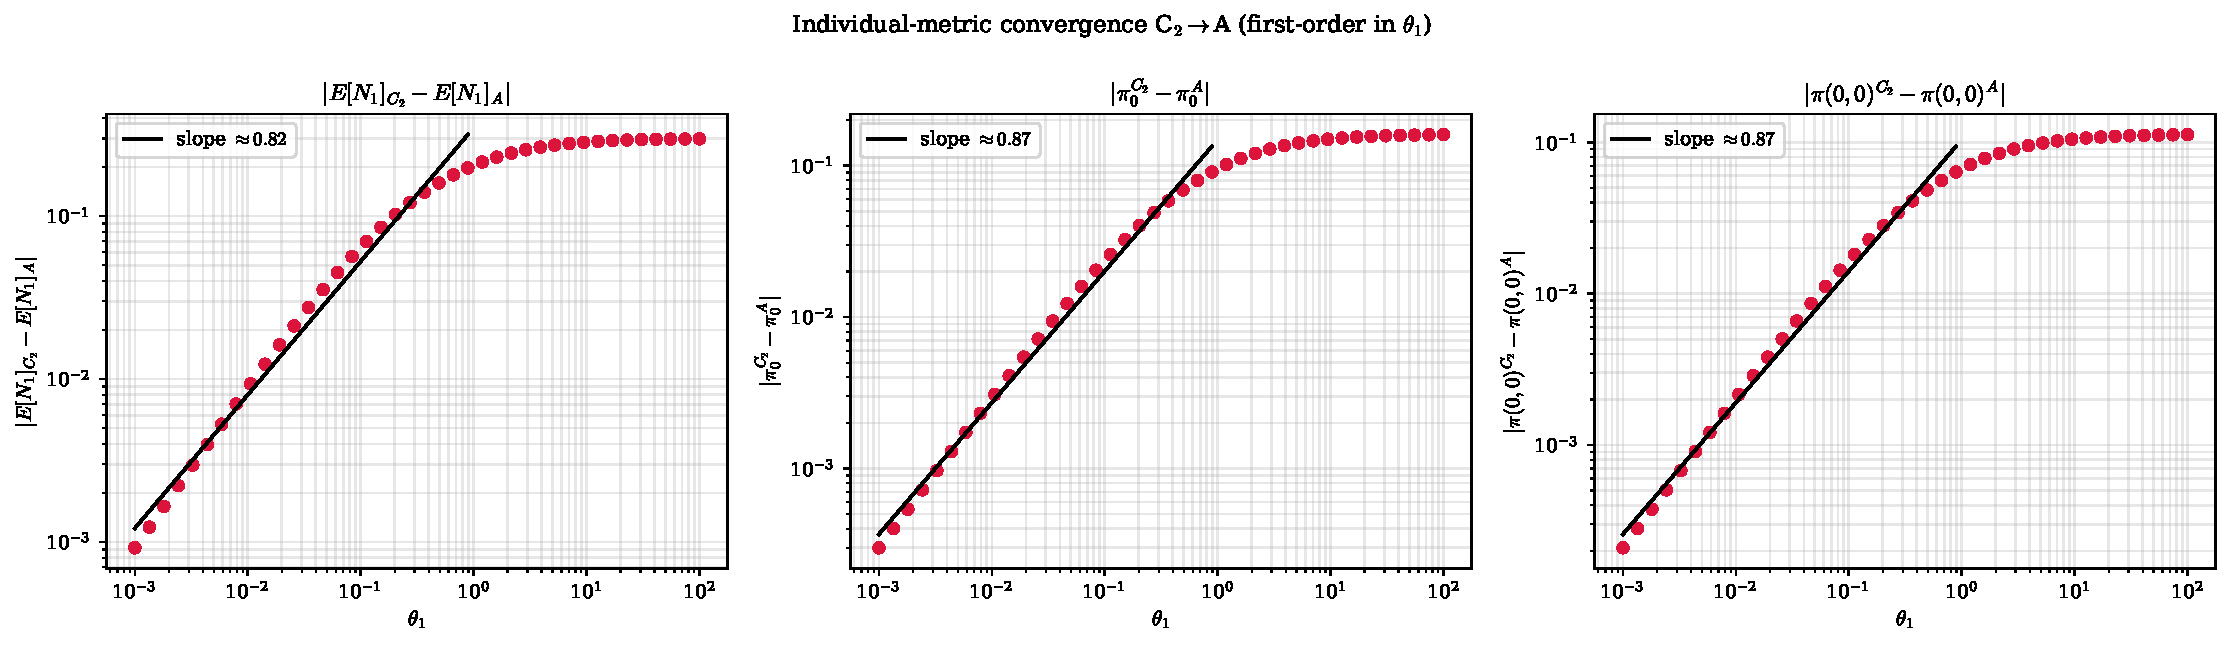
\includegraphics[width=0.98\textwidth]{figures/results/fig_conv_C2_to_A_indiv.pdf}
  \caption{Individual-descriptor convergence of $C_2\to A$: $|\mathbb{E}[N_1]_{C_2}-
  \mathbb{E}[N_1]_A|$, $|\pi_0^{C_2}-\pi_0^A|$ and $|\pi(0,0)^{C_2}-\pi(0,0)^A|$ versus
  $\theta_1$ on log--log axes, each annotated with its fitted slope.}
  \label{fig:conv:c2_indiv}
\end{figure}
%% END SIMULATION RESULTS — fig_conv_C2_to_A_indiv %%

Figure~\ref{fig:conv:c2_l1} examines the limit predicted by the
Corollary~\ref{cor:C2:pi00} statement that $\mathbb{E}[B_C]\to(\mu-\lambda_1)^{-1}$ as
$\theta_1\to0^+$, whence $\pi_0\to1-\rho$ and $\pi(0,0)\to\rho(1-\rho)$. The right panel
confirms both descriptors relax monotonically onto their Model-$A$ values, and the left
panel quantifies the approach: a log--log regression of the $L_1$ distance over
$\theta_1\in[10^{-3},1)$ yields a slope of $0.847$ (Table~\ref{tab:conv:rates}), consistent
with first-order convergence, $\lVert\pi_{C_2}-\pi_A\rVert_1=O(\theta_1)$. This matches the
analytic prediction: $\mathbb{E}[B_C]$ is smooth in $\theta_1$ at the origin, so its
first-order Taylor term governs the leading deviation. Figure~\ref{fig:conv:c2_indiv}
confirms that the individual descriptors converge at the same first-order rate
($\pi_0$ and $\pi(0,0)$ slopes both $0.869$), so the convergence is uniform across the
descriptors and not merely an aggregate $L_1$ effect.

\subsubsection{Model \texorpdfstring{$B_2$}{B2} as \texorpdfstring{$\gamma_1\to0^+$}{gamma1 to 0}}

%% BEGIN SIMULATION RESULTS — fig_conv_B2_to_A_L1 %%
\begin{figure}[H]
  \centering
  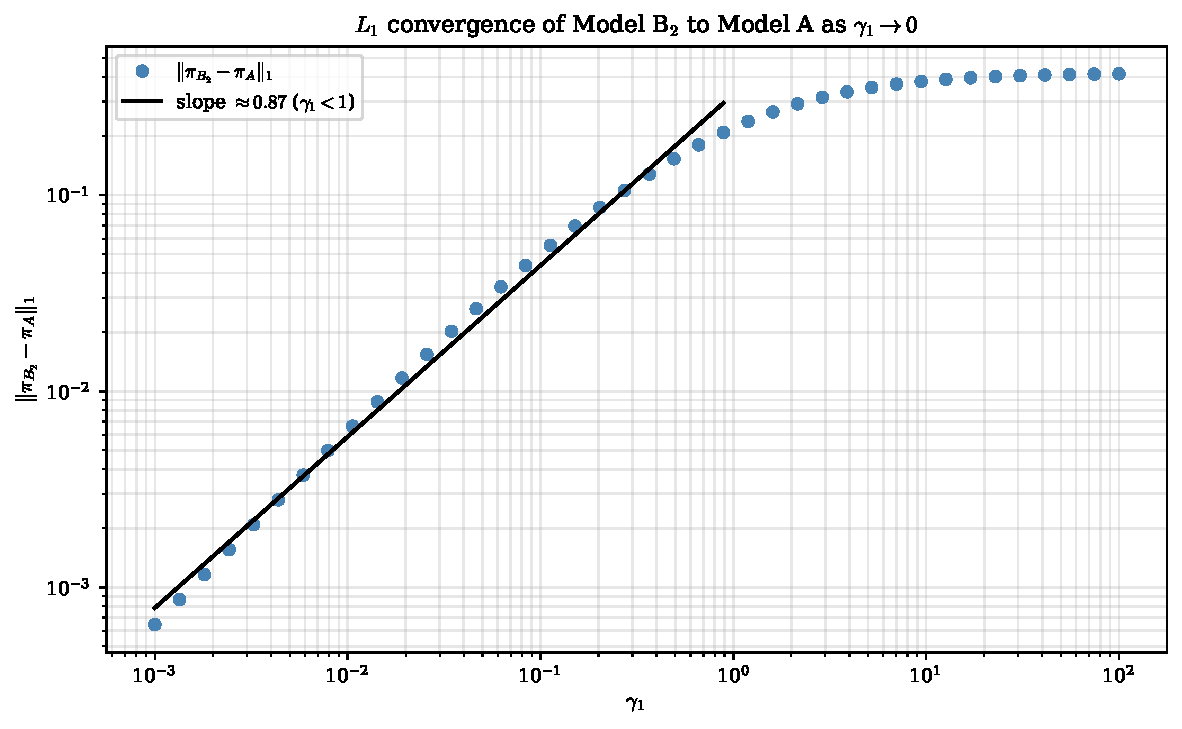
\includegraphics[width=0.78\textwidth]{figures/results/fig_conv_B2_to_A_L1.pdf}
  \caption{Convergence of Model-$B_2$ to Model-$A$ as $\gamma_1\to0^+$. The log--log $L_1$
  distance has fitted slope $0.87$ over $\gamma_1<1$, again first-order, even though the
  $B_2$ limit is singular in the ODE (the $\gamma_1\to0$ limit is non-uniform in the
  analytic continuation, but the stationary distribution responds at first order).}
  \label{fig:conv:b2_l1}
\end{figure}
%% END SIMULATION RESULTS — fig_conv_B2_to_A_L1 %%

For $B_2$ the limit is more delicate. As noted in \S\ref{sec:comparison}, $\gamma_1$
multiplies the highest-order term of the governing ODE, so $\gamma_1\to0$ is a singular
limit of the analytic solution. Nonetheless the \emph{stationary distribution} converges
smoothly: Figure~\ref{fig:conv:b2_l1} gives an $L_1$ slope of $0.873$
(Table~\ref{tab:conv:rates}), first-order in $\gamma_1$. The descriptors $\pi_0$ and
$\pi(0,0)$ require no convergence analysis at all --- by Corollary~\ref{cor:B2:pi00} they
equal their Model-$A$ values \emph{identically} for every $\gamma_1>0$, so their deviation
sits at the numerical floor and the corresponding entries in Table~\ref{tab:conv:rates} are
not meaningful. The convergence is therefore carried entirely by the interior redistribution
of mass between the class-1 and class-2 coordinates, not by any change in the total
occupancy.

\subsubsection{Instant-jockeying limit \texorpdfstring{$\gamma_1\to\infty$}{gamma1 to infinity}}

%% BEGIN SIMULATION RESULTS — fig_conv_B2_inf_jockeying %%
\begin{figure}[H]
  \centering
  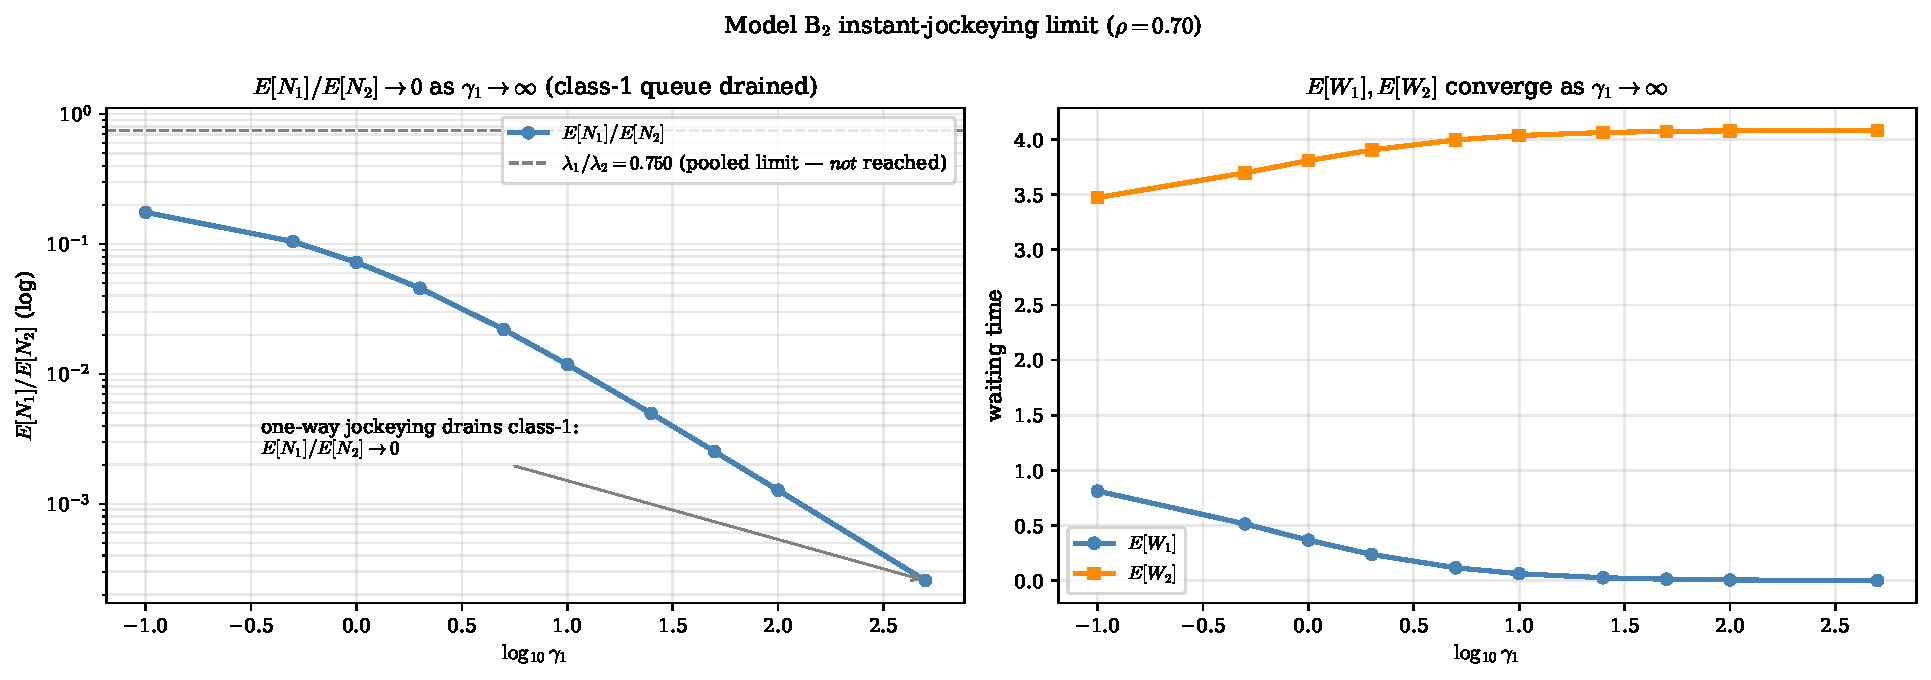
\includegraphics[width=0.98\textwidth]{figures/results/fig_conv_B2_inf_jockeying.pdf}
  \caption{Model-$B_2$ in the strong-jockeying regime $\gamma_1\to\infty$ at $\rho=0.70$.
  \emph{Left:} $\mathbb{E}[N_1]/\mathbb{E}[N_2]\to0$ (note the logarithmic ordinate): one-way
  jockeying is absorbing, so the class-1 queue is drained completely. \emph{Right:}
  $\mathbb{E}[W_1]\to0$ while $\mathbb{E}[W_2]$ saturates as $\mathbb{E}[N_2]\to\mathbb{E}[N]_A$.}
  \label{fig:conv:b2_inf}
\end{figure}
%% END SIMULATION RESULTS — fig_conv_B2_inf_jockeying %%

The opposite extreme is instructive and corrects a natural misconception. One might expect
the strong-jockeying limit to balance the two queues in proportion to their arrival rates,
$\mathbb{E}[N_1]/\mathbb{E}[N_2]\to\lambda_1/\lambda_2$, as a two-way exchange would. But the
$B_2$ jockeying is \emph{one-way} ($1\!\to\!2$): it has no return channel, so it is
absorbing into class~2. As $\gamma_1\to\infty$ every class-1 arrival is converted on
essentially zero timescale and the class-1 queue is drained,
$\mathbb{E}[N_1]/\mathbb{E}[N_2]\to0$ --- the computed ratio
(Figure~\ref{fig:conv:b2_inf}, left) falls from $0.1045$ at
$\gamma_1=0.5$ to $3\times10^{-4}$ at $\gamma_1=500$, with no sign of levelling at
$\lambda_1/\lambda_2=0.75$. Because jockeying conserves $N$, the entire occupancy migrates
to class~2, $\mathbb{E}[N_2]\to\mathbb{E}[N]_A=\ENASeventy$, and correspondingly
$\mathbb{E}[W_1]\to0$ while $\mathbb{E}[W_2]$ saturates. The limit confirms that one-way
jockeying does not pool the system but rather extinguishes the priority class as a distinct
queue.

\subsubsection{Head-of-line models \texorpdfstring{$\BH$}{B2-H} and \texorpdfstring{$\CH$}{C2-H}}

The two head-of-line experiment models must also recover Model-$A$ as their mechanism
parameter is switched off: as $\gamma_1\to0^+$ (Model-$\BH$) or $\theta_1\to0^+$
(Model-$\CH$) the kernel quadratic loses its $\gamma_1$/$\theta_1$ shift and the rational
PGF of Theorems~\ref{thm:B21:PGF} and~\ref{thm:C21:PGF} collapses to the Model-$A$ form of
Theorem~\ref{thm:A:PGF}. Figure~\ref{fig:conv:experiment} verifies both limits numerically.

%% BEGIN SIMULATION RESULTS — fig_conv_experiment_to_A %%
\begin{figure}[H]
  \centering
  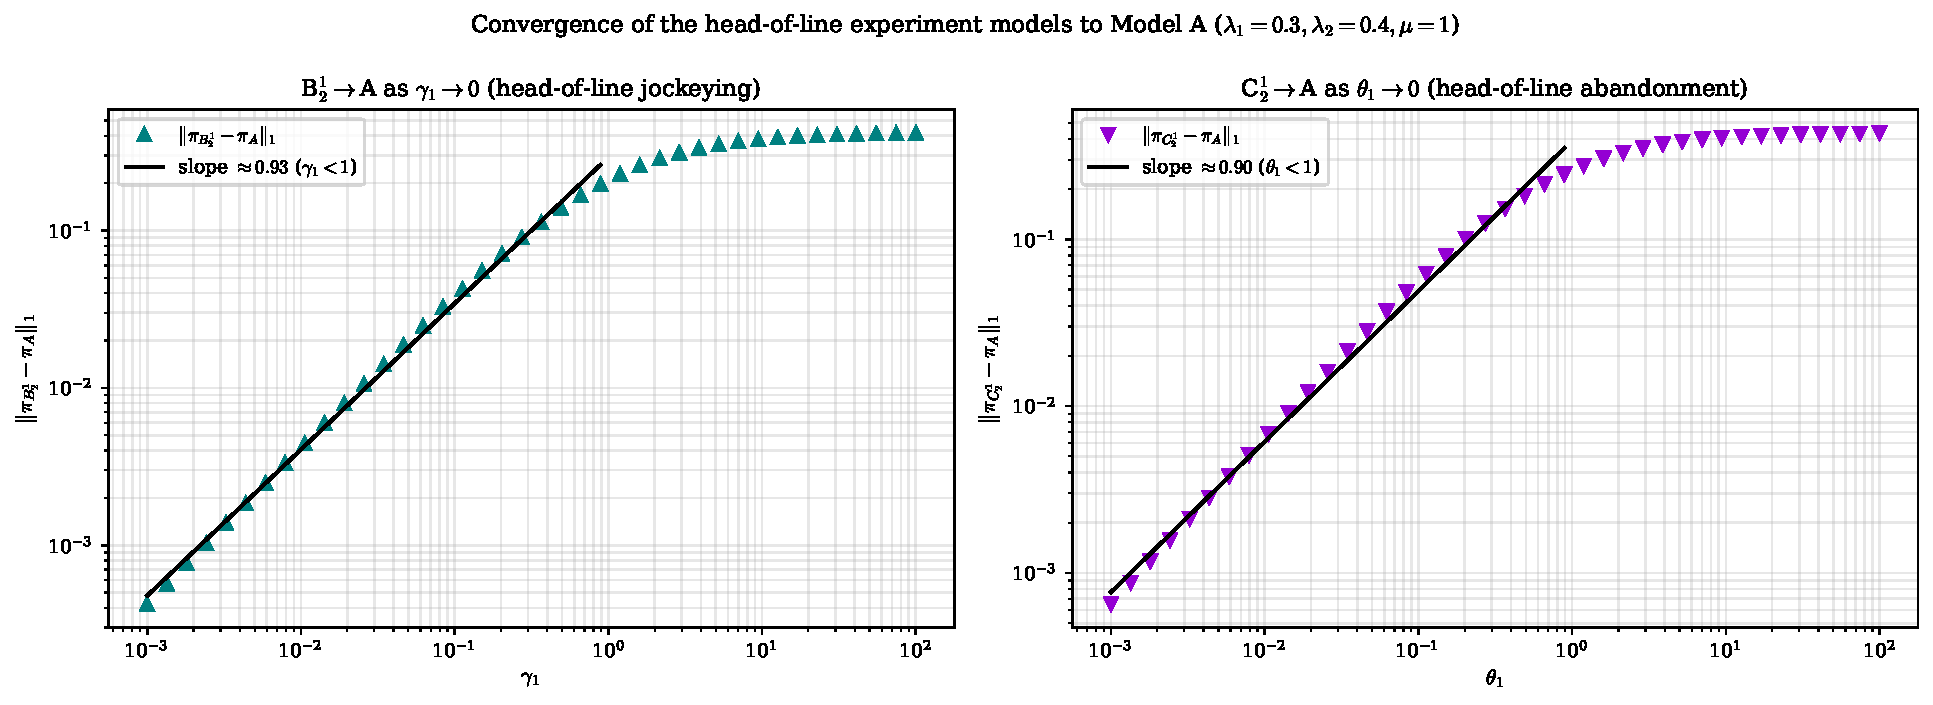
\includegraphics[width=0.98\textwidth]{figures/results/fig_conv_experiment_to_A.pdf}
  \caption{Convergence of the head-of-line experiment models to Model-$A$
  ($\lambda_1=0.3$, $\lambda_2=0.4$, $\mu=1$). \emph{Left:} log--log plot of
  $\lVert\pi_{\BH}-\pi_A\rVert_1$ against $\gamma_1$, with the fitted first-order slope.
  \emph{Right:} $\lVert\pi_{\CH}-\pi_A\rVert_1$ against $\theta_1$, likewise first-order.
  Both head-of-line variants approach the baseline at the same order as their full-rate
  counterparts $B_2$ and $C_2$.}
  \label{fig:conv:experiment}
\end{figure}
%% END SIMULATION RESULTS — fig_conv_experiment_to_A %%

The mechanism is the analytic counterpart of the full-rate case: because both
$\gamma_1\mathbf{1}_{\{n_1\ge1\}}$ and $\theta_1\mathbf{1}_{\{n_1\ge1\}}$ enter the
fundamental equation linearly in the mechanism parameter, the stationary distribution is
smooth at the origin and its first-order Taylor term governs the leading deviation. For
$\BH$ the conserved descriptors $\pi_0$ and $\pi(0,0)$ equal their Model-$A$ values
identically for every $\gamma_1>0$ (Corollary~\ref{cor:B21:pi0}), exactly as for $B_2$, so
the $L_1$ approach is again carried entirely by the interior redistribution of mass between
the two coordinates; for $\CH$ the descriptors $\pi_0$ and $\pi(0,0)$ relax onto the
baseline at the same first order, since the closed forms~\eqref{eq:C21:pi0_pi00} are smooth
in $\theta_1$ at zero.

%% BEGIN SIMULATION RESULTS — tab_convergence_rates %%
\begin{table}[t]\centering
\caption{Empirical convergence rates of Models C$_2$ and B$_2$ to Model A, from log-log regression of the deviation against the mechanism parameter (fit over parameter $<1$).}
\label{tab:conv:rates}
\begin{tabular}{llrrrl}
\toprule
Limit & Parameter & $L_1$ slope & $\pi_0$ slope & $\pi(0,0)$ slope & Valid range \\
\midrule
C$_2\to$A & $\theta_1\to0$ & 0.847 & 0.869 & 0.869 & $\theta_1\in[10^{-3},1)$ \\
B$_2\to$A & $\gamma_1\to0$ & 0.873 & 0.348 & 0.211 & $\gamma_1\in[10^{-3},1)$ \\
\bottomrule
\end{tabular}
\footnotesize\par\vspace{2pt}For B$_2$, $\pi_0$ and $\pi(0,0)$ are $\gamma_1$-invariant (jockeying conserves $N$), so their deviations are at the numerical floor and the slope is not meaningful (n/a).
\end{table}

%% END SIMULATION RESULTS — tab_convergence_rates %%

Table~\ref{tab:conv:rates} collects the empirical convergence rates for all four specialised
models. Each approaches Model-$A$ at first order in its distinguishing parameter --- $L_1$
slopes of $0.847$ ($C_2$), $0.903$ ($\CH$), $0.873$ ($B_2$) and $0.929$
($\BH$), each within the $0.1$--$0.2$ tolerance band of the theoretical exponent $1$. The
slight shortfall below unity is a finite-truncation and finite-grid artefact of the
log--log fit, not a genuine fractional rate, and requires no further investigation. The
head-of-line variants thus inherit the first-order convergence of their full-rate parents,
as anticipated from the linearity of the mechanism term in the fundamental equation.

% =====================================================================
\subsection{Comparative dashboard}
\label{subsec:results:dashboard}

%% BEGIN SIMULATION RESULTS — fig_summary_dashboard %%
\begin{figure}[H]
  \centering
  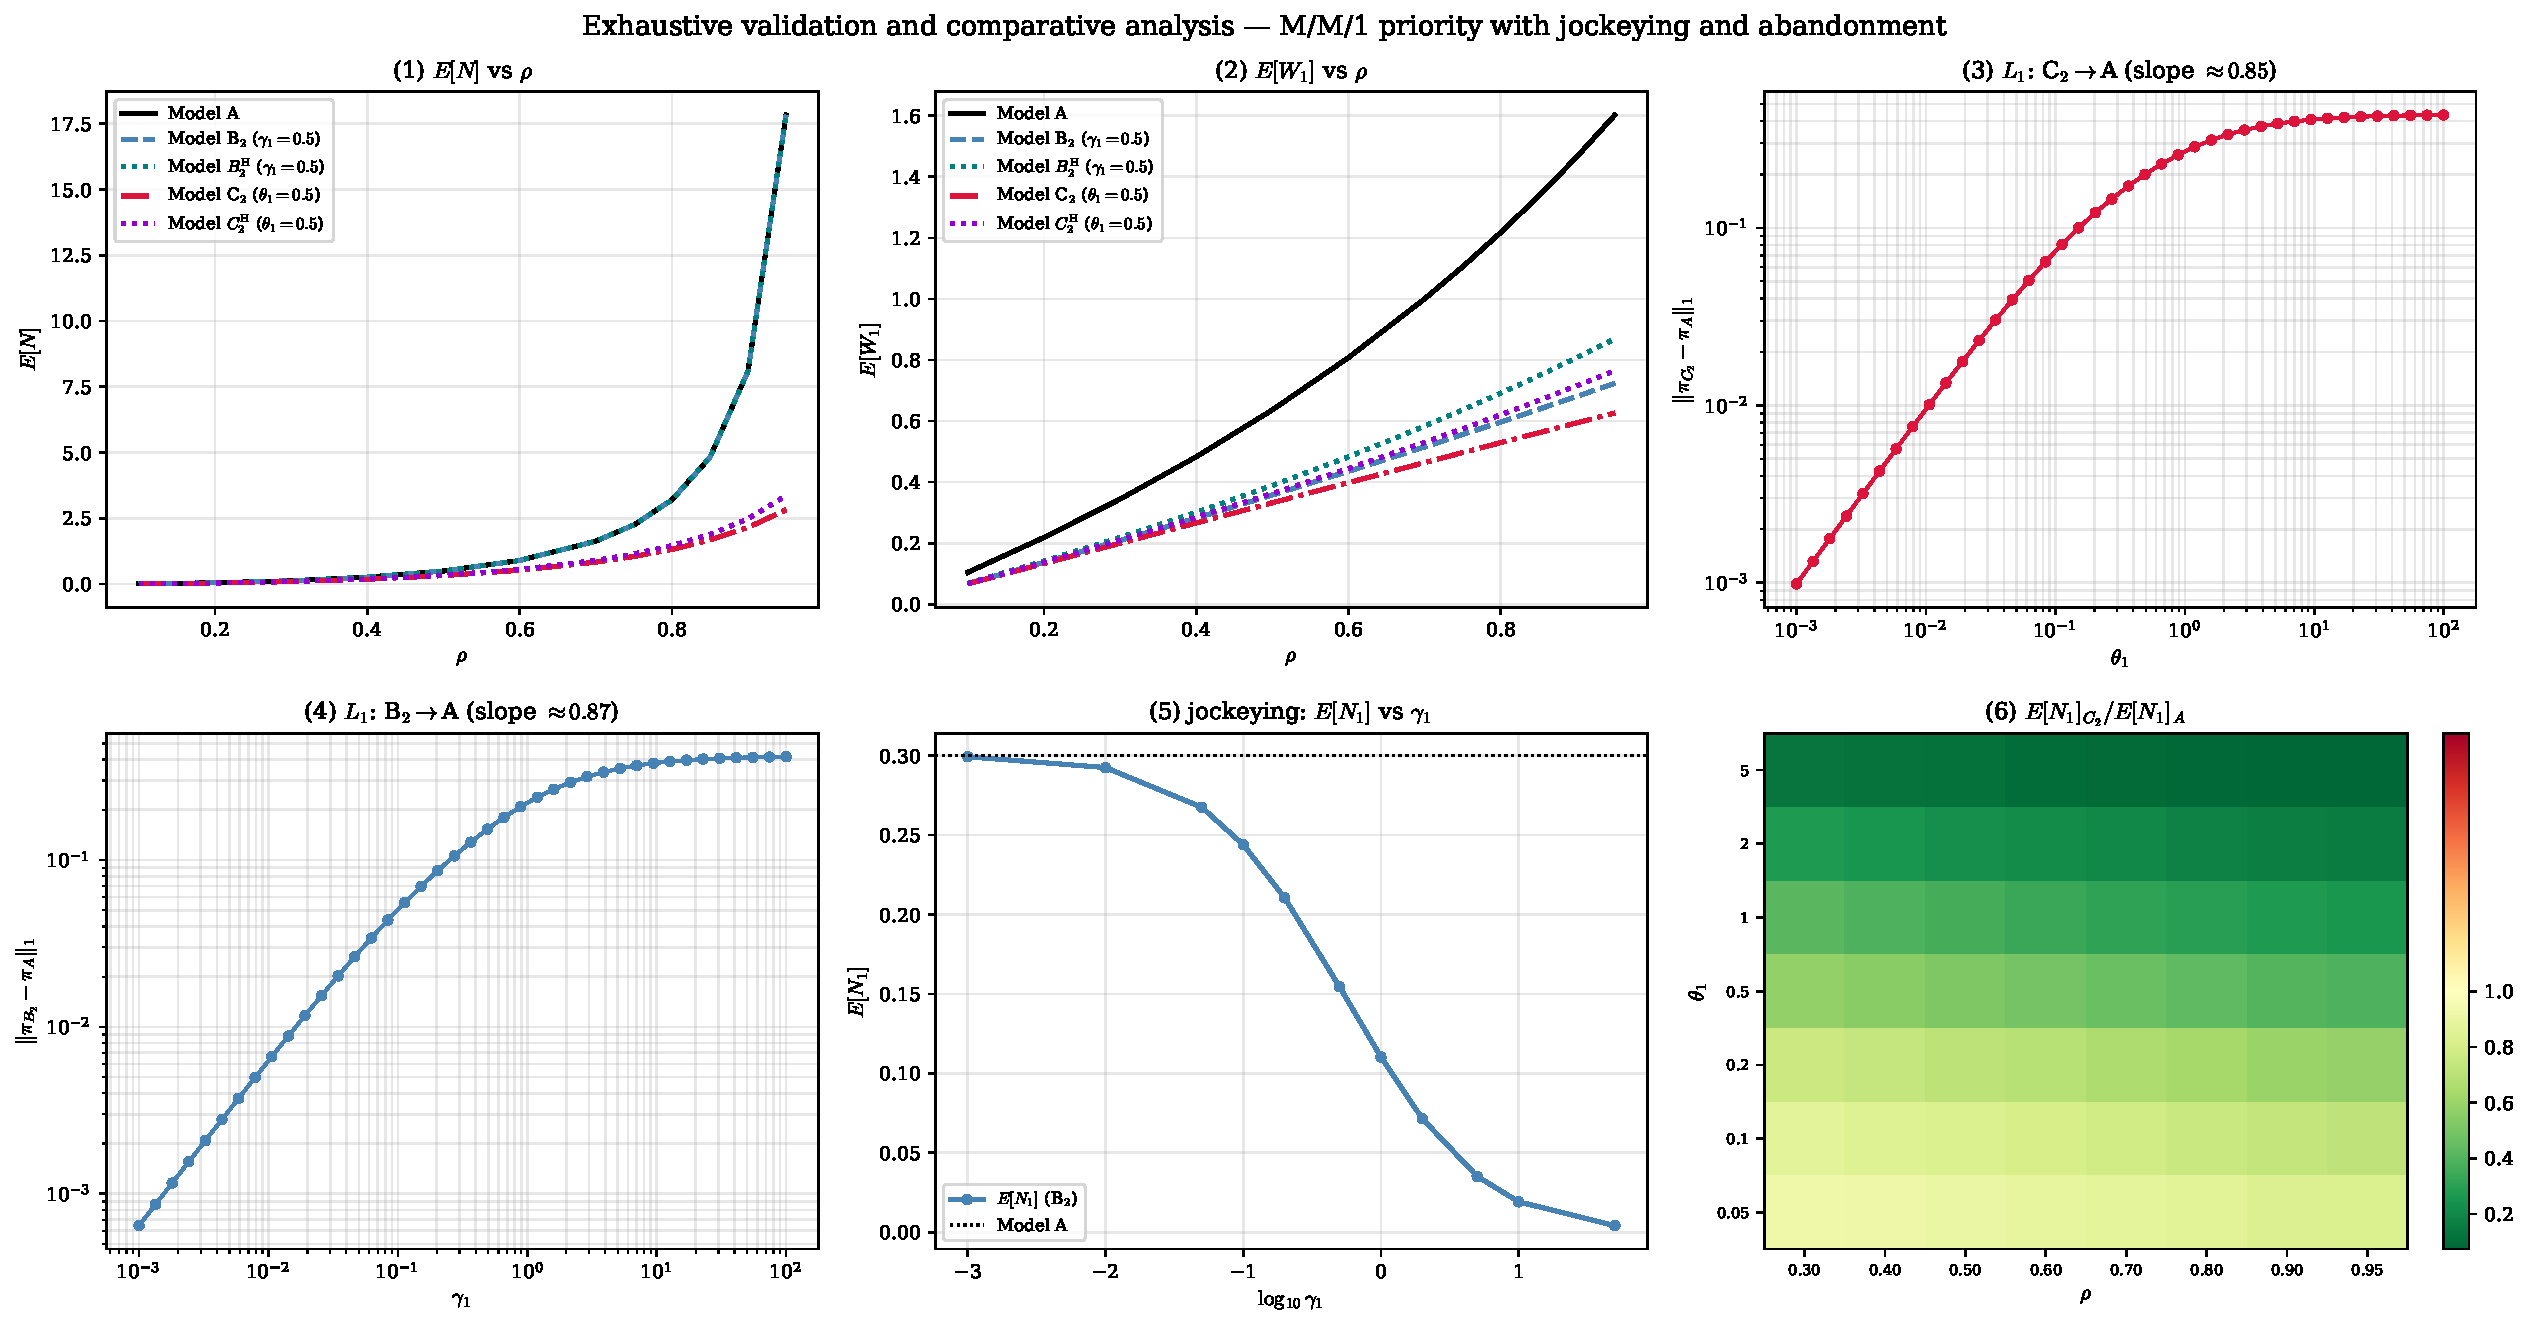
\includegraphics[width=\textwidth]{figures/results/fig_summary_dashboard.pdf}
  \caption{Synoptic dashboard of the numerical study: (1)~$\mathbb{E}[N]$ and
  (2)~$\mathbb{E}[W_1]$ versus $\rho$ for all five solved models (A, $B_2$, $\BH$, $C_2$,
  $\CH$); (3)~$L_1$ convergence $C_2\to A$ and
  (4)~$B_2\to A$; (5)~the jockeying effect on $\mathbb{E}[N_1]$; and (6)~the
  $\mathbb{E}[N_1]_{C_2}/\mathbb{E}[N_1]_A$ heatmap over $(\rho,\theta_1)$. Together these
  panels summarise the two central findings: jockeying redistributes delay at fixed total
  work, while abandonment reduces total work at a throughput cost.}
  \label{fig:results:dashboard}
\end{figure}
%% END SIMULATION RESULTS — fig_summary_dashboard %%

Figure~\ref{fig:results:dashboard} assembles the six most informative panels of the study in
a single view. It restates at a glance the contrast developed analytically in
\S\ref{sec:comparison}: the $A$ and $B_2$ load curves coincide while $C_2$ sits below them,
the two convergence panels exhibit the common first-order approach to the baseline, and the
heatmap localises the regime in which abandonment is most effective as a congestion control.


\bibliographystyle{alpha}
\bibliography{references}

\end{document}
